%%%%%%%%%%%%%%%%%%%%%%%%%%%%%%%%%%%%%%%%%%%%%%%%%%%%%%%%%%%%%%%%%
% Contents: Main Input File of the LaTeX2e Introduction
% $Id: lshort.tex,v 1.1.1.1 2002/02/26 10:04:21 oetiker Exp $
%%%%%%%%%%%%%%%%%%%%%%%%%%%%%%%%%%%%%%%%%%%%%%%%%%%%%%%%%%%%%%%%%
% lshort.tex - The not so short introduction to LaTeX
%                                                      by Tobias Oetiker
%                                                  tobias@ife.ee.ethz.ch
%                                                      oetiker@dmu.ac.uk
%
%                           based on LKURTZ.TEX Uni Graz & TU Wien, 1987
%-----------------------------------------------------------------------
%
% To compile lshort, you need TeX 3.x, LaTeX and makeindex
%
% The sources files of the Intro are:
%      lshort.tex (this file),
%      titel.tex, contrib.tex, biblio.tex
%      things.tes, typeset.tex, math.tex, lssym.tex, spec.tex,
%      lshort.sty, fancyheadings.sty
%
% Further the  verbatim.sty and the layout.sty
% from the LaTeX Tools distribution is
% required.
%
%
% To print the AMS symbols you need the AMS fonts and the packages
% amsfonts, eufrak and eucal from (AMS LaTeX 1.2)
%
% ---------------------------------------------------------------------

\ifx\printversion\undefined
\documentclass[12pt,oneside,openany]{book}
\else
\documentclass[a4paper,twoside]{book}
\usepackage[monochrome]{color}
\fi

\usepackage{lshort-vi}
\usepackage{makeidx,shortvrb,latexsym}
\usepackage{mylayout}

% are we in pdftex ????
%% \ifx\pdfoutput\undefined % We're not running pdftex
%% \else
%% \def\pdfBorderAttrs{/Border [0 0 0] } % No border around Links
%% \fi


\usepackage{amsmath,amssymb}
% \usepackage[pdftex,a4paper,twoside,headheight=20pt,top=2.5cm,bottom=2.5cm]{geometry}

% them vao de ho tro tieng Viet
%\usepackage[viscii]{inputenc}
% \usepackage[vietnam]{babel}
% \usepackage{ucs}
% \usepackage[utf8]{vietnam}

\makeindex
%\typeout{Copyright T.Oetiker, H.Partl, E.Schlegl, I.Hyna}

\usepackage[colorlinks,draft=false,hyperindex,plainpages=false,
pdftitle={The not so Short Introduction to LaTeX, Vietnamese edition},
pdfauthor={T. Oetiker, H. Partl, E. Schlegl, I. Hyna, Translator Nguyen
  Tan Khoa},
pdfsubject={LaTeX Manual},
pdfkeywords={LaTeX, typesetting}]{hyperref}
\ifx\printversion\undefined
\RequirePackage{thumbpdf}
\hypersetup{pdfpagemode=UseThumbs}
\fi
\input{pd1supp.def}

\begin{document}
\selectlanguage{vietnam}

\frontmatter
%%%%%%%%%%%%%%%%%%%%%%%%%%%%%%%%%%%%%%%%%%%%%%%%%%%%%%%%%%%%%%%%%
% Contents: The title page
% $Id: title.tex,v 1.2 2003/03/19 20:57:47 oetiker Exp $
%%%%%%%%%%%%%%%%%%%%%%%%%%%%%%%%%%%%%%%%%%%%%%%%%%%%%%%%%%%%%%%%%

\ifx\pdfoutput\undefined % We're not running pdftex
\else
\pdfbookmark{Title Page}{title}
\fi
\newlength{\centeroffset}
\setlength{\centeroffset}{-0.5\oddsidemargin}
\addtolength{\centeroffset}{0.5\evensidemargin}
%\addtolength{\textwidth}{-\centeroffset}
\thispagestyle{empty}
\vspace*{\stretch{1}}
\noindent\hspace*{\centeroffset}\makebox[0pt][l]{\begin{minipage}{\textwidth}
\flushright
{\Huge\bfseries Ne najkrajši\\ 
uvod v \LaTeXe

}
\noindent\rule[-1ex]{\textwidth}{5pt}\\[2.5ex]
\hfill\emph{\Large oziroma \LaTeXe{} v \pageref{verylast} minutah}
\end{minipage}}

\vspace{\stretch{1}}
\noindent\hspace*{\centeroffset}\makebox[0pt][l]{\begin{minipage}{\textwidth}
\flushright
{\bfseries 
Tobias Oetiker\\[1.5ex]
Hubert Partl, Irene Hyna in  Elisabeth Schlegl\\[3ex]} 
Version~4.20, May 31, 2006\\[6ex]
{\bfseries 
slovenski prevod in priredba\\[1.5ex]
Bor Plestenjak\\[1.5ex]}
Verzija~4.20.1, 12. november 2006
\end{minipage}}

%\addtolength{\textwidth}{\centeroffset}
\vspace{\stretch{2}}


\pagebreak
\begin{small} 
  Copyright \copyright 1995-2005 Tobias Oetiker and Contributers.  All rights reserved.
 
  Copyright \copyright 2006 Bor Plestenjak for the Slovene translation and adaptation. 
  All rights reserved.

  This document is free; you can redistribute it and/or modify it
  under the terms of the GNU General Public License as published by
  the Free Software Foundation; either version 2 of the License, or
  (at your option) any later version.
  
  This document is distributed in the hope that it will be useful, but
  WITHOUT ANY WARRANTY; without even the implied warranty of
  MERCHANTABILITY or FITNESS FOR A PARTICULAR PURPOSE\@.  See the GNU
  General Public License for more details.
  
  You should have received a copy of the GNU General Public License
  along with this document; if not, write to the Free Software
  Foundation, Inc., 675 Mass Ave, Cambridge, MA 02139, USA.

\end{small}
\vspace{6ex}

\begin{small} 
  Avtorske pravice \copyright 1995-2005 Tobias Oetiker in ostali, ki so prispevali k nastanku LShort. 
  Vse pravice pridržane.
 
  Avtorske pravice \copyright 2006 Bor Plestenjak za slovenski prevod in priredbo.
  Vse pravice pridržane.
 
  Ta dokument je prost; lahko ga prosto širite in/ali spreminjate pod
  pogoji navedenimi v splošni javni licenci GNU General Public License, ki jo je objavila 
  Free Software Foundation; ali različica 2 ali pa katera koli poznejša različica (po vaši izbiri).
  
  Ta dokument je na razpolago z upanjem, da bo uporaben, toda BREZ KAKRŠNEKOLI GARANCIJE;
  celo brez privzetega jamstva DA JE VREDEN UPORABE ali PRIMEREN ZA DOLOČEN NAMEN\@.  
  Za podrobnosti poglejte GNU General Public License.
  
  Poleg tega dokumenta bi morali prejeti tudi kopijo GNU General Public License; v nasprotnem primeru lahko pišete 
  na Free Software Foundation, Inc., 675 Mass Ave, Cambridge, MA 02139, USA.
\end{small}


\endinput

%

% Local Variables:
% TeX-master: "lshort2e"
% mode: latex
% mode: flyspell
% End:

%%%%%%%%%%%%%%%%%%%%%%%%%%%%%%%%%%%%%%%%%%%%%%%%%%%%%%%%%%%%%%%%%
% Contents: Who contributed to this Document
% $Id: contrib.tex 169 2008-09-24 07:32:13Z oetiker $
%%%%%%%%%%%%%%%%%%%%%%%%%%%%%%%%%%%%%%%%%%%%%%%%%%%%%%%%%%%%%%%%%
\chapter{��������}
\noindent �� ����� ������� ���������� ����� ��쳳���� ������ ��� ���� ��������� \LaTeX\ 2.09-��� ������ ����� ������� �� ������ �������:
\begin{verse}
\contrib{������� ����� (Hubert Partl)}{partl@mail.boku.ac.at}%
{��������� ������ ���� ���������� ������� ������ �� ���������� ���������� ����������� ����, ����}
\contrib{���� ���� (Irene Hyna)}{Irene.Hyna@bmwf.ac.at}%
   {������� ����� ���������� ���, ����}
\contrib{�������� ����� (Elisabeth Schlegl)}{�������}%
   {���� �����}
\end{verse}

������ ��� ����� �� �����, ���� �������� (J\"org Knappen) \LaTeXe{}-� ������� �������� ����������� ���������� \CTAN|info/lshort/german| ������� ����� ��� �����

\newpage \noindent ������ ���� ��쳳���� ����� ���㰰, ��������� ����� ������ ���������� ��� ������ ������ ����� ������ ���������� �������� ������ ������ ������� ����������� ������ �����. ����� ������� ����� ����� ����� ����� ������� ������, ����� ���������� ��������� ����� ����� ��쳳���� ������ ������ ��������.

{ \flushleft\small
Rosemary~Bailey,        %r.a.bailey@qmw.ac.uk 0.2
Marc~Bevand,            % <bevand_m@epita.fr>
Friedemann~Brauer,      %fbrauer@is.dal.ca 3.4
Barbara~Beeton,         %bnb@ams.org
Jan~Busa,               % <busaj@ccsun.tuke.sk>
Markus~Br\"uhwiler,     % <m.br@switzerland.org>
Pietro~Braione,         % <braione@elet.polimi.it>
David~Carlisle,         %GONE carlisle@cs.man.ac.uk 1.0
Jos\'e~Carlos~Santos,   % <jcsantos@fc.up.pt>
Neil~Carter,            % N.Carter@Swansea.ac.uk
Mike~Chapman,           %chapman@eeh.ee.ethz.ch 3.16
Pierre~Chardaire,       % <pc@sys.uea.ac.uk
Christopher~Chin,       %chris.chin@rmit.edu.au 3.1
Carl~Cerecke,           %cdc@cosc.canterbury.ac.nz>
Chris~McCormack,        %GONE chrismc@eecs.umich.edu 0.1
Wim~van~Dam,            %GONE wimvdam@cs.kun.nl 2.2
Jan~Dittberner,         %jan@jan-dittberner.de 3.15
Michael~John~Downes,    %<mjd@ams.org> 14 Oct 1999
Matthias~Dreier,        %dreier@ostium.ch
David~Dureisseix,       %dureisse@lmt.ens-cachan.fr 1.1
Elliot,                 %GONE enh-a@minster.york.ac.uk 1.1
Hans~Ehrbar,            %ehrbar@econ.utah.edu
Daniel~Flipo,           %Daniel.Flipo@univ-lille1.fr
David~Frey,             %david@eos.lugs.ch 2.2
Hans~Fugal,             %hans@fugal.net
Robin~Fairbairns,       %Robin.Fairbairns@cl.cam.ac.uk 0.2 1.0
J\"org~Fischer,        %j.fischer@xpoint.at 3.16
Erik~Frisk,             %frisk@isy.liu.se 3.4
Mic~Milic~Frederickx,   % <mic.milic@web.de>
Frank,                  %frank@freezone.co.uk 11 Feb 2000
Kasper~B.~Graversen,    % <kbg@dkik.dk>
Arlo~Griffiths,         % <A.Griffiths@let.leidenuniv.nl>
Alexandre~Guimond,      %guimond@IRO.UMontreal.CA 0.9
Andy~Goth,              % <unununium@openverse.com>
Cyril~Goutte,           %goutte@ei.dtu.dk 2.1 2.2
Greg~Gamble,            %gregg@maths.uwa.edu.au 2.2
Frank~Fischli,          % <fischlifaenger@gmx.ch>
Morten~H{\o}gholm,		% morten.hoegholm@latex-project.org
Neil~Hammond,           %nfh@dmu.ac.uk 0.3
Rasmus~Borup~Hansen,    %GONE rbhfamos@math.ku.dk 0.2 0.9 0.91 0.92 1.9.9
Joseph~Hilferty,        % <hilferty@fil.ub.es>
Bj\"orn Hvittfeldt,     %bjorn@hvittfeldt.com 3.13
Martien~Hulsen,         %M.A.Hulsen@WbMt.TUDelft.NL 1.0 1.1
Werner~Icking,          %<Werner.Icking@gmd.de> 3.1
Jakob,                  %diness@get2net.dk
Eric~Jacoboni,          %GONE jacoboni@enseeiht.fr 0.1 0.9
Alan~Jeffrey,           %alanje@cogs.sussex.ac.uk 0.2
Byron~Jones,            %bj@dmu.ac.uk 1.1
David~Jones,            %GONE djones@CA.McMaster.dcss.insight 1.1
Johannes-Maria~Kaltenbach, %<kaltenbach@zeiss.de> 3.01
Michael~Koundouros,     % <mkoundouros@hotmail.com>
Andrzej~Kawalec,        %GONE akawalec@prz.rzeszow.pl 1.9.9
Sander~de~Kievit,       %Skievit@ucu.uu.nl
Alain~Kessi,            %ALAIN_KESSI@HOTMAIL.COM 2.2
Christian~Kern,         %ck@unixen.hrz.uni-oldenburg.de 2.1
Tobias~Klauser,		%tklauser@access.unizh.ch 4.17
J\"org~Knappen,         %knappen@vkpmzd.kph.uni-mainz.de 0.1
Kjetil~Kjernsmo,        %<kjetil.kjernsmo@astro.uio.no> 3.2
Maik~Lehradt,           %greek@uni-paderborn.de 0.1
R\'emi~Letot,           % <r_letot@yahoo.com>
Flori~Lambrechts,       % <f.lambrechts@softhome.net>
Axel~Liljencrantz,	% <Axel.Liljencrantz@byv.kth.se>
Johan~Lundberg,         %p99jlu@physto.se
Alexander~Mai,          %Alexander.Mai@physik.tu-darmstadt.de 3.8
Hendrik~Maryns,         %hendrik.maryns@ugent.be
Martin~Maechler,        %<maechler@stat.math.ethz.ch> 2.2
Aleksandar~S~Milosevic, % <aleksandar.milosevic@yale.edu>
Henrik~Mitsch,          % <Henrik.Mitsch@gmx.at>
Claus~Malten,           %GONE <ASI138%BITNET.DJUKFA11@BITNET.CEARN> 1.1
Kevin~Van~Maren,        % <vanmaren@fast.cs.utah.edu>  24 Nov 1999
Richard~Nagy,           % r.nagy@nameshield.net
Philipp~Nagele,         % Philipp.Nagele@t-systems.com
Lenimar~Nunes~de~Andrade, % <lenimar@mat.ufpb.br> Fri, 12 Nov 1999
Manuel~Oetiker,         % manuel@oetiker.ch
Urs~Oswald,             % osurs@bluewin.ch
Lan~Thuy~Pham,          %<lan.thuy.pham@gmail.com>
Martin~Pfister,		% m@rtinpfister.ch
Demerson~Andre~Polli,   % polli@linux.ime.usp.br
Nikos~Pothitos,		% <n.pothitos@di.uoa.gr>
Maksym~Polyakov         % <polyama@myrealbox.com>
Hubert~Partl,           %partl@mail.boku.ac.at 0.2 1.1
John~Refling,           %refling@sierra.lbl.gov 0.1 0.9
Mike~Ressler,           %ressler@cougar.jpl.nasa.gov 0.1 0.2 0.9 1.0 1.9.9
Brian~Ripley,           %ripley@stats.ox.ac.uk 2.1
Young~U.~Ryu,           %ryoung@utdallas.edu 2.1
Bernd~Rosenlecher,      %9rosenle@informatik.uni-hamburg.de 10 Feb 2000
Kurt~Rosenfeld,		%kurt@isis.poly.edu
Chris~Rowley,           %C.A.Rowley@open.ac.uk 0.91
Risto~Saarelma,         %risto.saarelma@cs.helsinki.fi
Hanspeter~Schmid,       %schmid@isi.ee.ethz.ch
Craig~Schlenter,        %cschle@lucy.ee.und.ac.za 0.1 0.2 0.9
Gilles~Schintgen,       %gschintgen@internet.lu
Baron~Schwartz,         % <bps7j@cs.virginia.edu>
Christopher~Sawtell,    %<csawtell@xtra.co.nz> 1 Sep 1999
Miles~Spielberg,        %zeibach@hotmail.com
Matthieu~Stigler,       % table row height
Geoffrey~Swindale,      % <geofftswin@ntlworld.com>
Laszlo~Szathmary,       % <szathml@delfin.klte.hu>
Boris~Tobotras,         % <tobotras@jet.msk.su>
Josef~Tkadlec,          %tkadlec@math.feld.cvut.cz 2.0 2.2
Scott~Veirs,            %scottv@ocean.washington.edu
Didier~Verna,           %verna@inf.enst.fr 2.2
Fabian~Wernli,          %wernli@iap.fr 3.2
Carl-Gustav~Werner,     % <Carl-Gustav.Werner@math.lu.se> 11 Oct 1999,3.16
David~Woodhouse,        % <dwmw2@infradead.org> 3.16
Chris~York,             % <c.s.york@Cummins.com>  21 Nov 1999
Fritz~Zaucker,          %zaucker@ee.ethz.ch 3.0
Rick~Zaccone,           %zaccone@bucknell.edu 2.2
����� Mikhail~Zotov.      %zotov@eas.npi.msu.su 3.1

}

\vspace*{\stretch{1}}



\pagebreak
\endinput
%

% Local Variables:
% TeX-master: "lshort2e"
% mode: latex
% mode: flyspell
% End:

%%%%%%%%%%%%%%%%%%%%%%%%%%%%%%%%%%%%%%%%%%%%%%%%%%%%%%%%%%%%%%%%%
% Contents: Who contributed to this Document
% $Id: overview.tex 456 2011-04-06 09:10:27Z oetiker $
%%%%%%%%%%%%%%%%%%%%%%%%%%%%%%%%%%%%%%%%%%%%%%%%%%%%%%%%%%%%%%%%%

% Because this introduction is the reader's first impression, I have
% edited very heavily to try to clarify and economize the language.
% I hope you do not mind! I always try to ask "is this word needed?"
% in my own writing but I don't want to impose my style on you...
% but here I think it may be more important than the rest of the book.
% --baron

\chapter{Eessõna}

\LaTeX{} \cite{manual} on küljendussüsteem, mis sobib väga hästi
tüpograafiliselt kõrge kvaliteediga teaduslike ja matemaatiliste
dokumentide loomiseks. Kuid ta sobib ka igasuguste muude tekstide
vormistamiseks, lihtsatest kirjadest täiemahuliste raamatuteni.
Trükiladumiseks kasutab \LaTeX{} programmi~\TeX{}~\cite{texbook}.

Käesolev lühike sissejuhatus kirjeldab süsteemi \LaTeXe{} ja peaks olema
piisav enamiku \LaTeX i-rakenduste jaoks. Täieliku ülevaate \LaTeX ist
võib leida raamatutest~\cite{manual,companion}.

\bigskip
\noindent See sissejuhatus jaguneb 6 peatükiks.
\begin{description}
\item[1. peatükk] kirjeldab \LaTeXe{} dokumentide põhistruktuuri, samuti
  puudutab veidi \LaTeX i ajalugu. Selle peatüki läbilugemisel peaks
  tekkima üldine ettekujutus, kuidas \LaTeX{} töötab.
\item[2. peatükk] süveneb dokumentide küljendamise üksikasjadesse ning
  tutvustab enamikku olulisemaid \LaTeX i käske ja keskkondi. Pärast
  selle peatüki lugemist saab hakata koostama esimesi dokumente.
\item[3. peatükk] selgitab, kuidas panna \LaTeX is kirja valemeid,
  illustreerides seda \LaTeX i ühte tugevaimat külge paljude näidetega.
  Peatüki lõpus asuvad tabelid, kuhu on koondatud kõik \LaTeX is
  kättesaadavad matemaatilised sümbolid.
\item[4. peatükk] tutvustab aineregistreid, kirjandusnimestiku
  genereerimist ja EPS-graafika lisamist. Siin käsitletakse ka
  PDF-dokumentide loomist pdf\LaTeX iga ning tuuakse välja mõned
  kasulikud lisapaketid.
\item[5. peatükk] näitab, kuidas \LaTeX iga luua graafikat. Selle
  asemel, et joonistada mõne joonistusprogrammiga pilt, salvestada see
  faili ja lisada dokumendile, võib \LaTeX ile ette anda pildi
  kirjelduse ja lasta tal endal selle järgi pilt valmis joonistada.
\item[6. peatükk] sisaldab veidi ohtlikuvõitu informatsiooni
  selle kohta, kuidas \LaTeX i standardset dokumendikujundust muuta.
  Siin selgitatakse, kuidas korraldada asju ümber nii, et
  \LaTeX i kaunis väljund muutuks koledaks või imeliseks, vastavalt
  kujundaja oskustele.
\end{description}
\bigskip
\noindent
Oluline on lugeda peatükke just selles järjekorras -- nii mahukas see
raamat ka pole. Hoolikalt tuleks läbi lugeda näited, sest palju
informatsiooni on koondatud raamatus leiduvatesse näidetesse.

\bigskip
\noindent \LaTeX{} on saadaval enamiku arvutite jaoks PC-st ja Macist
suurte UNIXi ja VMSi süsteemideni. Paljude ülikoolide arvutivõrkudes on
\LaTeX{} juba installitud ja kasutamiseks valmis. Juhiseid kohalikule
\LaTeX i-installatsioonile juurdepääsemise kohta annab \guide. Kui tekib
probleeme alustamisega, siis tasub küsida abi inimeselt, kes selle
raamatu andis. Käesoleva juhendi eesmärk \emph{ei ole} selgitada,
kuidas \LaTeX i installida ja üles seada, vaid õpetada, kuidas
kirjutada dokumente nii, et \LaTeX{} oskaks neid töödelda.

\bigskip
\noindent Ükskõik millise \LaTeX iga seotud materjali leidmiseks võib
esimesena vaadata mõnda CTANi (Comprehensive \TeX{} Archive
Network) saiti. CTANi kodulehekülg on \url{http://www.ctan.org}.

Siin raamatus leidub muidki viiteid CTANile, eeskätt allalaaditavatele
programmidele ja dokumentidele. Täieliku URLi asemel on nendes
aadressiks lihtsalt \texttt{CTAN:} koos järgneva asukohaga CTANi puus,
kuhu tuleks minna.

Oma arvutis \LaTeX i töölepanemiseks leiab materjali kataloogist
\CTAN|tex-archive/systems|.

\vspace{\stretch{1}}
\noindent Kui selle dokumendi kohta tekib mõtteid, st mida võiks lisada,
kustutada või muuta, siis palun need lahkesti mulle saata. Iseäranis
olen huvitatud tagasisidest algajatelt \LaTeX i-kasutajatelt selle
kohta, millised osad olid siin sissejuhatuses kergesti mõistetavad ja
mis võiks olla selgitatud paremini.

\bigskip
\begin{verse}
\contrib{Tobias Oetiker}{tobi@oetiker.ch}%
\noindent{OETIKER+PARTNER AG\\Aarweg 15\\4600 Olten\\\v{S}veits}
\end{verse}
\vspace{\stretch{1}}
\noindent Käesoleva dokumendi viimane versioon asub aadressil
\CTAN|tex-archive/info/lshort|.

\endinput



%

% Local Variables:
% TeX-master: "lshort2e"
% mode: latex
% mode: flyspell
% End:


\tableofcontents
\listoffigures
\listoftables

\enlargethispage{\baselineskip}
\mainmatter

%%%%%%%%%%%%%%%%%%%%%%%%%%%%%%%%%%%%%%%%%%%%%%%%%%%%%%%%%%%%%%%%%
% Contents: Things you need to know
% $Id: things.tex 536 2015-06-26 06:41:33Z oetiker $
%%%%%%%%%%%%%%%%%%%%%%%%%%%%%%%%%%%%%%%%%%%%%%%%%%%%%%%%%%%%%%%%%

\chapter{Asjad, mida tuleks teada}
\begin{intro}
Peatüki esimeses pooles anname lühikese ülevaate \LaTeXe{} filosoofiast
ja ajaloost. Teises pooles keskendume \LaTeX i-dokumendi
põhistruktuurile. Selle peatüki läbilugemisel peaks tekkima \LaTeX i
töötamisest üldine arusaam, mida läheb vaja raamatu ülejäänud osa
mõistmiseks.
\end{intro}

\section{Nimed}
\subsection{\TeX}

\TeX{} on \index{Knuth, Donald E.}Donald E. Knuthi kirjutatud
arvutiprogramm \cite{texbook} teksti ja valemite ladumiseks. Knuth
alustas trükiladumisprogrammi \TeX{} loomist aastal 1977, et uurida
võimalusi, mida pakkusid tol ajal kirjastamistööstuses levima hakanud
digitaalsed trükiseadmed, iseäranis lootuses pöörata ümber
trüki"-kvaliteedi järkjärguline langus, mida ta nägi omaenda raamatute ja
artiklite peal. \TeX{} sellisel kujul, nagu me teda tänapäeval kasutame,
valmis aastal 1982. Väikesi täiendusi tehti veel 1989. aastal, kui
parandati 8-bitiste märkide ja mitmekeelsuse tuge. \TeX i kuulsus
põhineb sellel, et ta on äärmiselt stabiilne, töötab paljudel
arvutitüüpidel ja on sama hästi kui veavaba. \TeX i versiooninumber
läheneb arvule $\pi$ ja on praegu $3{,}141592653$.

Nime \TeX{} hääldatakse kui "`tehh"', kus "`hh"' hääldub nagu saksa
sõnas \emph{ach}\footnote{Saksa keeles on \emph{ch} hääldamiseks õieti
kaks viisi ja võiks arvata, et \emph{ch} pehme hääldus sõna \emph{Pech}
moodi on sobivam. Sellekohasele küsimusele vastas Knuth saksa Vikipeedia
andmetel: "`Ma ei pahanda, kui inimesed hääldavad sõna \TeX{} nii, nagu
neile meeldib [\,-\,-\,-\,] ning Saksamaal ütlevad paljud pehme "`ch"',
sest X järgneb vokaalile e, mitte kõva "`ch"', mis järgneb vokaalile a.
Vene keeles on sõna \emph{tex} väga tavaline ja hääldub nagu "`tjeh"'.
Kuid ma usun, et kõige sobivam hääldus on kreeka keeles, kus "`ch"' on
kaledam nagu sõnades \emph{ach} ja \emph{loch}."'} või \v{s}oti sõnas
\emph{loch}. Hääldus "`hh"' tuleneb kreeka tähestikust, kus X on täht h
ehk hii. \TeX{} on ka kreeka sõna {\greektext teqnik'h} `tehnika'
esimene silp. ASCII-keskkonnas kirjutatakse \TeX{} kujul \texttt{TeX}.

\subsection{\LaTeX}

\LaTeX{} on makrode pakett, mis võimaldab autoritel oma kirjatööd
vormistada ja trükkida kõige kõrgemal tüpograafilisel kvaliteeditasemel,
rakendades eeldefineeritud professionaalset kujundust. \LaTeX i on
loonud \index{Lamport, Leslie}Leslie Lamport~\cite{manual} ning see
kasutab ladumismootorina küljendusprogrammi \TeX. Praegusel ajal haldab
\LaTeX i \index{Mittelbach, Frank}Frank Mittelbach.

%In 1994 the \LaTeX{} package was updated by the \index{LaTeX3@\LaTeX
%  3}\LaTeX 3 team, led by \index{Mittelbach, Frank}Frank Mittelbach,
%to include some long-requested improvements, and to re\-unify all the
%patched versions which had cropped up since the release of
%\index{LaTeX 2.09@\LaTeX{} 2.09}\LaTeX{} 2.09 some years earlier. To
%distinguish the new version from the old, it is called \index{LaTeX
%2e@\LaTeXe}\LaTeXe. This documentation deals with \LaTeXe. These days you
%might be hard pressed to find the venerable \LaTeX{} 2.09 installed
%anywhere.

\LaTeX{} hääldub kui "`La-tehh"' või "`Lei-tehh"'. ASCIIs
kirjutatakse \LaTeX{} kujul \texttt{LaTeX}. \LaTeXe{}
hääldatakse "`La-tehh kaks e"' ja kirjutatakse \texttt{LaTeX2e}.

%Figure~\ref{components} above % on page \pageref{components}
%shows how \TeX{} and \LaTeXe{} work together. This figure is taken from
%\texttt{wots.tex} by Kees van der Laan.

%\begin{figure}[btp]
%\begin{lined}{0.8\textwidth}
%\begin{center}
%\input{kees.fig}
%\end{center}
%\end{lined}
%\caption{Components of a \TeX{} System.} \label{components}
%\end{figure}

\section{Põhialused}

\subsection{Autor, kujundaja ja laduja}

Käsikirja avaldamiseks annab autor selle kirjastamisfirmale. Firma
kujundaja paneb seejärel paika teose kujunduse (veerulaius, kirjatüübid,
vahed enne ja pärast pealkirja,~\ldots). Kujundaja kirjutab oma juhised
käsikirjale ja annab selle siis ladujale, kes teose vastavalt nendele
juhistele valmis laob.

Inimkujundaja püüab aru saada, mida autor käsikirja kirjutamise ajal
mõtles. Peatükkide pealkirjade, viidete, näidete, valemite jne üle
otsustab ta oma professionaalsete teadmiste ja käsikirja sisu põhjal.

\LaTeX i keskkonnas on kujundaja rollis \LaTeX{} ja ladujaks \TeX. Kuid
et \LaTeX{} on "`ainult"' programm, vajab ta seetõttu rohkem abi. Autor
peab talle andma täiendavat informatsiooni, kirjeldades teose loogilist
struktuuri. See informatsioon kirjutatakse teksti sisse "`\LaTeX i
käskudena"'.

Selline lähenemine erineb üsnagi
\index{visuaalredaktorid}visuaalredaktorite\footnote{\wi{WYSIWYG}
(\emph{What you see is what you get} `Mida näed, seda saad').} omast,
mida järgib enamik tänapäeva tekstitöötlusprogramme, nagu \wi{MS Word}
ja \wi{LibreOffice}. Nendes programmides määrab autor dokumendi
kujunduse interaktiivselt teksti sisestamise käigus. Autor näeb
ekraanil, kuidas teos prindituna paistab.

\LaTeX i puhul autor lõppväljundit tavaliselt teksti kirjutamise ajal ei
näe, kuid lõppväljundit saab vaadata ekraanil pärast faili töötlemist
\LaTeX iga. Siis on võimalik enne printimist teha dokumendis parandusi.

\subsection{Küljenduse kujundus}

Tüpograafiline kujundamine on oskustöö. Oskusteta autorid teevad tihti
tõsiseid vormistamisvigu eeldades, et teose kujundamine on eeskätt
esteetika küsimus: "`Kui dokument näeb ilus välja, siis on ta hästi
kujundatud"'. Aga kuivõrd dokument on mõeldud lugemiseks, mitte seinale
riputamiseks, on loetavus ja arusaadavus palju olulisemad kui ilus
välimus. Näiteks:\enlargethispage{1.3\baselineskip}
\begin{itemize}
\item pealkirjade kirjasuurus ja nummerdus tuleb valida nii, et
  peatükkide ja jaotiste struktuur oleks lugejale selge;
\item reapikkus peab olema piisavalt väike, et mitte lugeja silmi
  kurnata, samas aga piisavalt suur, et lehekülg kenasti täita.
\end{itemize}

Visuaalredaktoritega\index{visuaalredaktorid} loovad kasutajad tihti
esteetiliselt kauneid dokumente, millel struktuur peaaegu puudub või
pole kooskõlaline. \LaTeX{} ennetab selliseid vormistusvigu, sest sunnib
autorit kirjeldama dokumendi \emph{loogilist} struktuuri ja valib selle
järgi ise kõige sobivama kujunduse.

\subsection{Eelised ja puudused}

Kui visuaalredaktorite ja \LaTeX i kasutajad omavahel kokku saavad,
tekib tihti arutelu teemal "`\index{LaTeXi eelised@\LaTeX i
eelised}\LaTeX i eelised tavalise tekstitöötlusprogrammi ees"' või
vastupidi. Kui selline arutelu käivitub, siis on kõige parem hoida
madalat profiili, sest sageli kipuvad need mõttevahetused käest ära
minema. Kuid mõnikord ei ole pääsu \ldots

Seega on siin natuke laskemoona. \LaTeX i peamised eelised tavaliste
tekstitöötlusprogrammide ees on järgmised.
\begin{itemize}
\item Saab kasutada professionaalseid kujundusi, tänu millele näeb
  dokument välja tõesti nagu "`trükitud"'.
\item Valemite vormistamine on mugav.
\item Vaja on selgeks õppida ainult mõned lihtsasti arusaadavad
  käsud, mis määravad ära dokumendi loogilise struktuuri. Peaaegu mitte
  kunagi pole vaja jännata dokumendi tegeliku kujundusega.
\item Lihtsasti saab luua ka keerulisi struktuure nagu allmärkusi,
  ristviiteid, sisukordi ja kirjandusnimestikke.
\item Tüpograafiliste ülesannete jaoks, mida baas-\LaTeX{} ei toeta, on
  olemas vabalt kasutatavad lisapaketid. Näiteks on olemas paketid
  dokumenti \PSi i graafika lisamiseks ja kindlat standardit järgivate
  kirjandusnimestike vormistamiseks. Paljusid neist pakettidest on
  kirjeldatud raamatus \companion.
\item \LaTeX{} soodustab hea struktuuriga tekstide kirjutamist, sest see
  on viis, kuidas \LaTeX{} töötab -- struktuuri määrates.
\item \LaTeXe{} ladumismootor \TeX{} on väga portatiivne ja vaba.
  Seetõttu töötab süsteem peaaegu igal riistvaraplatvormil.
%
% Add examples ...
%
\end{itemize}

\LaTeX il on samuti mõningaid puudusi. Ma arvan, et minul on veidi raske
leida ühtki mõistlikku, kuid olen kindel, et teised suudavad neid välja
tuua sadu \texttt{;-)}
\begin{itemize}
\item \LaTeX{} ei aita eriti inimesi, kes on müünud oma hinge
  \ldots
\item Kuigi valmis dokumendikujundustes saab sättida
  mõningaid parameetreid, on terve uue kujunduse loomine raske ja võtab
  palju aega.\footnote{Kuuldused räägivad, et see on üks
  peamistest küsimustest, mida puudutab valmiv \LaTeX 3
  süsteem.}\index{LaTeX3@\LaTeX 3}
\item Väga raske on kirjutada struktureerimata ja organiseerimata
  tekste.
\item Lubavatest esimestest sammudest hoolimata ei tarvitse sinu
  lemmikhamster kunagi täielikult mõista loogilise märgendamise
  põhimõtet.
\end{itemize}

\section{\LaTeX i sisendfailid}

\LaTeX i sisendiks\index{sisendfail} on tavaline tekstifail.
Unixis/Linuxis on tekstifailid üsna tavalised. Windowsis saab
tekstifaile moodustada Notepadiga. Sisendfail sisaldab nii teose teksti
kui ka käske, mis ütlevad \LaTeX ile, kuidas teksti vormistada. Kui
tegutseda \LaTeX i integreeritud keskkonnas, siis on seal olemas
vahendid tekstivormingus sisendfaili loomiseks \LaTeX i jaoks.

\subsection{Tühikud}

"`Tühisümboleid"' nagu tühikut ja tabulatsioonimärki käsitleb \LaTeX{}
ühtviisi \wi{tühik}una. \emph{Mitu järjestikust} \wi{tühisümbol}it
loetakse \emph{üheks} tühikuks. Rea alguses olevat tühikut üldiselt
ignoreeritakse ja ühte reavahetust loetakse samuti
tühikuks.\index{tühik!rea alguses}

Tühi rida kahe tekstirea vahel märgib lõigu lõppu. \emph{Mitu} tühja
rida on sama mis \emph{üks} tühi rida. Seda illustreerib järgmine näide.
Vasakul on sisendfaili tekst ja paremal vormindatud väljund.

\begin{example}
Pole oluline, kas
sõna järele lisada üks
või mitu       tühikut.

Tühi rida alustab uut
lõiku.
\end{example}

\subsection{Erimärgid}

Järgmised märgid on \wi{reserveeritud sümbolid}, millel on \LaTeX is kas
eritähendus või pole nad kõigis kirjades kättesaadavad. Kui sisestada
need märgid otse teksti, siis tavaliselt neid ei trükita, vaid nad
panevad \LaTeX i tegema asju, mida kasutajal ilmselt polnud plaanis.
\begin{code}
\verb.#  $  %  ^  &  _  {  }  ~  \ . %$
\end{code}
Nagu edaspidi näeme, saab neid märke siiski teksti lisada, kui kirjutada
nende ette \wi{langjoon}:
\begin{example}
\# \$ \% \^{} \& \_ \{ \} \~{}
\textbackslash
\end{example}

Teisi sümboleid ja palju muud saab trükkida erikäskudega
valemire\v{z}iimis või diakriitiliste märkidena.
\index{langjoon}Langjoone märki \textbackslash{} \emph{ei saa} sisestada
teist langjoont selle ette lisades (\verb|\\|); see märgijärjend on
mõeldud rea murdmiseks. Selle asemel võib kasutada käsku
\ci{textbackslash}.

\subsection{\LaTeX i käsud}

\LaTeX i \index{käsk}käsud on tõstutundlikud ning nad esinevad
emmal-kummal järgmisest kahest kujust.

\begin{itemize}
\item Käsk algab \wi{langjoon}ega \verb|\| ja sellele järgneb ainult
tähtedest koosnev nimi. Käsu nime lõpetab tühik, number või ükskõik
milline muu mittetäht.
\item Käsk koosneb langjoonest ja täpselt ühest mittetähest.
\end{itemize}

Paljudel käskudel on olemas ka tärnkuju, mille puhul käsu nime järele on
lisatud tärn.\index{käsk!tärniga}\index{tärniga käsk}

%
% \\* doesn't comply !
%

%
% Can \3 be a valid command ? (jacoboni)
%
\label{whitespace}

\LaTeX{} ignoreerib tühikuid käskude järel. Kui on vaja panna käsu
järele \index{tühik!käsu järel}tühik, tuleb käsu nime järele kirjutada
kas tühi argument \verb|{}| ja tühik või siis spetsiaalne tühja vahe
käsk. Tühi argument \verb|{}| ei lase \LaTeX il pärast käsu nime
tulevaid tühikuid ära süüa.

\begin{example}
Algajatel võib \TeX tühikud käsu
järel vahele jätta. % valesti
Edasijõudnutele \TeX{} sobib, sest
nemad on \TeX perdid ja teavad,
kuidas tühikuid lisada. % õigesti
\end{example}

Mõned käsud nõuavad \index{argument}argumenti, mis tuleb anda
\index{looksulud}looksulgudes \verb|{ }| pärast käsu nime. Mõned käsud
tunnistavad ka \index{valikuline
argument}\index{argument!valikuline}valikulist argumenti, mis lisatakse
käsu nime järele \index{nurksulud}nurksulgudes~\verb|[ ]|.
\begin{code}
\verb|\|\textit{käsk}\verb|[|\textit{valikuline argument}\verb|]{|\textit{argument}\verb|}|
\end{code}
Järgmistes näidetes on kasutatud mõningaid \LaTeX i käske. Nende pärast
pole vaja muretseda, neid selgitatakse hiljem.

\begin{example}
Sa võid mulle \textsl{toetuda}!
\end{example}
\begin{example}
Palun alusta uut rida
just siit!\newline
Tänan!
\end{example}

\subsection{Kommentaarid}
\index{kommentaarid}

Kui \LaTeX{} kohtab sisendfaili töödeldes protsendimärki
\index}\verb|%|, siis ignoreerib ta käsiloleva rea
ülejäänud osa, reavahetust ja kõiki tühisümboleid järgmise rea alguses.
Nii saab sisendfaili kirjutada märkusi, mis trükiversioonis ei ilmu.

\begin{example}
See on % rumal
% Parem: õpetlik <----
näide: kuulilen%
              nuteetun%
    neliluuk
\end{example}

Märgi \verb|%| abil saab ka tükeldada pikki sisendridu, kus tühikud ega
reavahetused pole lubatud.

Pikemate kommentaaride jaoks on olemas keskkond \ei{comment} paketist
\pai{verbatim}. Selle keskkonna kasutamiseks tuleb dokumendi
preambulisse lisada rida \verb|\usepackage{verbatim}|, nagu selgitatakse
edaspidi.

\begin{example}
See on üks teine
\begin{comment}
üsna rumal,
kuid kasulik
\end{comment}
näide kommentaaride
lisamisest dokumenti.
\end{example}
\noindent See ei tööta keerulisemate keskkondade sees, nagu
valemikeskkond.

\section{Sisendfaili struktuur}
\label{sec:structure}\index{sisendfail}
Kui \LaTeXe{} töötleb sisendfaili, siis eeldab ta, et see järgib
teatavat \index{sisendfaili struktuur}struktuuri. Sellest tulenevalt
peab iga sisendfail algama käsuga\cih{documentclass}
\begin{code}
\verb|\documentclass{...}|
\end{code}
See määrab, mis liiki dokumendiga on tegu. Selle järel tulevad käsud,
mis mõjutavad kogu dokumendi välimust, või loevad sisse \wi{pakett}e,
mis lisavad \LaTeX i süsteemile uusi võimalusi. Pakett loetakse sisse
käsuga\cih{usepackage}
\begin{code}
\verb|\usepackage{...}|
\end{code}

Kui kogu seadistustöö on tehtud,\footnote{Käskude \texttt{\bs
documentclass} ja \texttt{\bs begin$\mathtt{\{}$document$\mathtt{\}}$}
vahele jäävat dokumendi osa nimetatakse \emph{\wi{preambul}iks}.} siis
algab dokumendi põhisisu käsuga
\begin{code}
\verb|\begin{document}|
\end{code}
Nüüd võib sisestada teksti vaheldumisi igasuguste kasulike \LaTeX i
käskudega. Dokumendi lõppu pannakse käsk
\begin{code}
\verb|\end{document}|
\end{code}
mis ütleb \LaTeX ile, et töö on läbi. Kõike, mis veel järgneb, \LaTeX{}
ignoreerib.

Joonisel~\ref{mini} on kujutatud minimaalse \LaTeX i faili sisu. Veidi
keerukam \wi{sisendfail} on joonisel~\ref{document}.\index{sisendfail}

\begin{figure}[tp]
\begin{lined}{6cm}
\begin{verbatim}
\documentclass{article}
\begin{document}
Minimaalne on ilus.
\end{document}
\end{verbatim}
\end{lined}
\caption{Minimaalne \LaTeX i fail} \label{mini}
\end{figure}

\begin{figure}[tp]
\begin{lined}{10cm}
\begin{verbatim}
\documentclass[a4paper,11pt]{article}
% seadistused eesti keele jaoks
\usepackage[estonian]{babel}
\usepackage[utf8]{inputenc}
\usepackage[T1]{fontenc}
% määra pealkiri
\author{H.~Partl}
\title{Minimalism}
\begin{document}
% moodustab pealkirja
\maketitle
% lisab sisukorra
\tableofcontents
\section{Mõned huvitavad sõnad}
Nii, siin algab minu armas artikkel.
\section{Nägemiseni}
\ldots{} ja siin ta lõpeb.
\end{document}
\end{verbatim}
\end{lined}
\caption[Realistliku ajakirjaartikli näide]{Realistliku ajakirjaartikli
näide. Kõiki selles näites esinevaid käske tutvustame hiljem.}
\label{document}

\end{figure}

\section{Tüüpiline käsureasessioon}

Arvatavasti on nüüd tekkinud suur tahtmine leheküljel \pageref{mini}
olevat kena väikest \LaTeX i sisendfaili ise järele proovida. Siin on
veidi juhiseid: \LaTeX il endal puuduvad graafiline liides ja peened
vajutatavad nupud. Ta on lihtsalt programm, mis töötleb sisendfaili.
Mõnes \LaTeX i installatsioonis on olemas graafiline kasutajaliides, kus
sisendfaili kompileerimiseks on olemas nupp \LaTeX. Teistes süsteemides
võib olla vaja midagi klaviatuurilt trükkida, seega näitame siin, kuidas
meelitada \LaTeX i kompileerima sisendfaili tekstipõhises süsteemis.
Tähelepanu: see kirjeldus eeldab, et arvutis on olemas töötav \LaTeX i
installatsioon.\footnote{See on nii enamikus hästi hallatud Unixi
süsteemides ning \ldots{} Tõelised Mehed kasutavad Unixit, nii et
\ldots{} \texttt{;-)}}

\begin{enumerate}
\item

Ava/loo \LaTeX i sisendfail. See fail peab olema lihtne ASCII tekst.
Unixis teevad kõik tekstiredaktorid just seda. Windowsis tuleks hoolt
kanda, et fail salvestatakse ASCII või lihtteksti vormingus. Faili nime
valides tuleks jälgida, et laiendiks saaks \eei{tex}.

\item

Ava käsurida või \texttt{cmd} aken, mine kataloogi, kus sisendfail asub,
ja käivita \LaTeX{} sisendfailil.
\begin{lscommand}
\verb+latex foo.tex+
\end{lscommand}
Õnnestumise korral tekib töö tulemusena fail laiendiga \eei{dvi}.
Vajalik võib olla sisendfail \LaTeX ist läbi lasta mitu korda, et
sisukord ja kõik ristviited õigeks muutuksid. Kui sisendfailis on mõni
viga, siis teatab \LaTeX{} sellest ja peatab faili töötlemise. Vajuta
Ctrl+D, et käsureale tagasi saada.

\item

Nüüd võib \wi{DVI-fail}i vaadata. Selleks on mitu võimalust. Faili
vaatamiseks ekraanil on käsk\index{Xdvi}
\begin{lscommand}
\verb+xdvi foo.dvi &+
\end{lscommand}
See töötab ainult Unixis X11-ga. Windowsis võib proovida programmi
\wi{Yap} (\emph{Yet another previewer}).

Võib ka teisendada DVI-faili \PSi iks, mida saab printida või vaadata
\wi{Ghostscript}iga, andes
käsu\index{dvips@\texttt{dvips}}\index{PS-fail}
\begin{lscommand}
\verb+dvips -Pcmz foo.dvi -o foo.ps+
\end{lscommand}

Kui veab, siis võib \LaTeX i süsteem sisaldada isegi tööriista
\index{dvipdf@\texttt{dvipdf}}\texttt{dvipdf}, millega saab DVI-faili
teisendada otse PDF-iks.\index{PDF-fail}
\begin{lscommand}
\verb+dvipdf foo.dvi+
\end{lscommand}

\end{enumerate}

\section{Dokumendi kujundus}

\subsection {Dokumendiklassid}\label{sec:documentclass}

Esimene informatsioon, mida \LaTeX{} sisendfaili töötlemisel vajab, on
loodava dokumendi liik. See määratakse käsuga \ci{documentclass}.
\begin{lscommand}
\ci{documentclass}\verb|[|\emph{suvandid}\verb|]{|\emph{klass}\verb|}|
\end{lscommand}
\noindent Argument \emph{klass} määrab dokumendi liigi.
Tabelis~\ref{documentclasses} on loetletud dokumendiklassid, mida
käesolevas sissejuhatuses mainitakse. \LaTeXe{} distributsiooni
kuulub muidki dokumendiklasse, sealhulgas klassid kirjade ja esitluste
jaoks. Argument \index{suvand}\emph{suvandid} täpsustab dokumendiklassi
käitumist. Suvandid tuleb üksteisest eraldada komadega. Standardsete
dokumendiklasside kõige tavalisemad suvandid on kirjas
tabelis~\ref{options}.

\begin{table}[!bp]
\caption{Dokumendiklassid} \label{documentclasses}
\begin{lined}{\textwidth}
\begin{description}

\item [\normalfont\pai{article}] teadusajakirjade artiklid,
  ettekanded, lühiaruanded, programmidokumentatsioon, infolehed, \ldots{}
  \index{klass!article@\textsf{article}}
\item [\normalfont\pai{proc}] artikliklassil põhinevate dokumentide
  kogumikud (toimetised). \index{klass!proc@\textsf{proc}}
\item [\normalfont\pai{minimal}] nii väike kui saab olla. Määrab
  ainult tekstiploki mõõtmed ja põhikirja tüübi. Kasutatakse peamiselt
  silumise eesmärgil. \index{klass!minimal@\textsf{minimal}}
\item [\normalfont\pai{report}] pikemad mitmepeatükilised aruanded,
  väiksemad raamatud, väitekirjad, \ldots{}
  \index{klass!report@\textsf{report}}
\item [\normalfont\pai{book}] päris raamatud.
  \index{klass!book@\textsf{book}}
\item [\normalfont\pai{slides}] slaidid. Tekstikirjaks on suur
  seriifideta kiri. Slaidide jaoks on eelistatum klass \pai{beamer}.
  \index{klass!slides@\textsf{slides}}\index{klass!beamer@\textsf{beamer}}
\end{description}
\end{lined}
\end{table}

\begin{table}[tp]
\caption{Dokumendiklasside suvandid} \label{options}
\begin{lined}{\textwidth}
% \begin{flushleft}
\begin{description}
\item[\normalfont\texttt{10pt}, \texttt{11pt}, \texttt{12pt}] \quad
  Määrab dokumendi põhikirja suuruse. Kui suvandit pole antud, siis
  võetakse selleks \texttt{10pt}.%
  \index{kirjasuurus}\index{dokumendi kirjasuurus}\index{põhikirja suurus}%
  \index{10pt@\texttt{10pt}}\index{11pt@\texttt{11pt}}\index{12pt@\texttt{12pt}}

\item[\normalfont\texttt{a4paper}, \texttt{letterpaper}, \ldots] \quad
  Määrab paberi formaadi. Vaikeformaat on \texttt{letterpaper}. Veel on
  olemas \texttt{a5paper}, \texttt{b5paper}, \texttt{executivepaper} ja
  \texttt{legalpaper}.
  \index{paberi formaat}%
  \index{formaat!A4}\index{formaat!letter}\index{formaat!A5}%
  \index{formaat!B5}\index{formaat!executive}\index{formaat!legal}%
  \index{a4paper@\texttt{a4paper}}\index{letterpaper@\texttt{letterpaper}}%
  \index{a5paper@\texttt{a5paper}}\index{b5paper@\texttt{b5paper}}%
  \index{executivepaper@\texttt{executivepaper}}\index{legalpaper@\texttt{legalpaper}}

\item[\normalfont\texttt{fleqn}] \quad Rajastab eraldi real olevad
  valemid vasakule, mitte keskele.
  \index{fleqn@\texttt{fleqn}}

\item[\normalfont\texttt{leqno}] \quad Paneb valeminumbrid valemist
  vasakule, mitte paremale.
  \index{leqno@\texttt{leqno}}

\item[\normalfont\texttt{titlepage}, \texttt{notitlepage}] \quad Määrab,
  kas pärast dokumendi \index{tiitel}tiitlit alustada uut lehekülge või
  mitte. Klass \pai{article} vaikimisi ei alusta uut lehekülge,
  klassid \pai{report} ja \pai{book} alustavad. \index{tiitel}
  \index{titlepage@\texttt{titlepage}}\index{notitlepage@\texttt{notitlepage}}

\item[\normalfont\texttt{onecolumn}, \texttt{twocolumn}] \quad Küljendab
  dokumendi teksti \index{üheveeruline trükk}ühes veerus või
  \index{kaheveeruline trükk}kahes veerus.
  \index{onecolumn@\texttt{onecolumn}}\index{twocolumn@\texttt{twocolumn}}

\item[\normalfont\texttt{twoside}, \texttt{oneside}] \quad Määrab, kas
  genereerida kahepoolselt või ühepoolselt trükitavate lehekülgedega
  väljund. Vaikimisi on klassid \pai{article} ja \pai{report}
  \index{ühepoolne trükk}ühepoolsed, klass \pai{book} aga
  \index{kahepoolne trükk}{kahepoolne}. See suvand puudutab ainult
  dokumendi stiili. Suvand \texttt{twoside} \emph{ei anna} kasutatavale
  printerile korraldust printida dokument välja kahepoolselt.
  \index{oneside@\texttt{oneside}}\index{twoside@\texttt{twoside}}

\item[\normalfont\texttt{landscape}] \quad Muudab dokumendi kujunduse
  sobivaks rõhtpaigutuses printimise jaoks.
  \index{landscape@\texttt{landscape}}\index{rõhtpaigutus}

\item[\normalfont\texttt{openright}, \texttt{openany}] \quad Seab peatükid algama
  kas ainult parempoolsel leheküljel või järgmisel vabal leheküljel. Ei
  tööta klassiga \pai{article}, mis peatükke ei tunne. Vaikimisi
  algavad peatükid klassis \pai{report} järgmisel vabal leheküljel ja
  klassis \pai{book} parempoolsel leheküljel.
  \index{openright@\texttt{openright}}\index{openany@\texttt{openany}}

\end{description}
% \end{flushleft}
\end{lined}
\end{table}

Näiteks võib \LaTeX i sisendfail alata reaga
\begin{code}
\ci{documentclass}\verb|[11pt,twoside,a4paper]{article}|
\end{code}
Sellega vormistab \LaTeX{} dokumendi \emph{artiklina} põhikirja
suurusega \emph{11 punkti} küljenduses, mis sobib
\emph{kahepoolseks} printimiseks \emph{A4-lehele}.

\subsection{Paketid}
\index{pakett}Dokumenti kirjutades võib mõnes valdkonnas ilmneda
probleeme, mida baas-\LaTeX{} lahendada ei suuda. Kui on vaja dokumenti
lisada graafikat, moodustada värvilist teksti või lugeda failist sisse
programmi lähtekoodi, siis tuleb \LaTeX i võimeid laiendada. Selliseid
laiendusi nimetatakse pakettideks. Pakett võetakse kasutusele käsuga
\begin{lscommand}
\ci{usepackage}\verb|[|\emph{suvandid}\verb|]{|\emph{pakett}\verb|}|
\end{lscommand}
\noindent kus \emph{pakett} on paketi nimi ja \emph{suvandid} nimekiri
võtmesõnadest, mis käivitavad paketis spetsiaalseid funktsioone. Käsk
\ci{usepackage} pannakse dokumendi preambulisse. Täpsemalt vaadeldi seda
jaotises \ref{sec:structure}.

Mõned paketid tulevad kaasa \LaTeXe{} baasdistributsiooniga (vt
tabelit~\ref{packages}), teised on saadaval eraldi. Oma arvutisse
installitud pakettide kohta peaks rohkem infot andma \guide. Põhiline
infoallikas \LaTeX i pakettide kohta on \companion, mis sisaldab sadade
pakettide kirjeldusi, samuti juhiseid, kuidas \LaTeXe{} jaoks ise
laiendusi kirjutada.

Kaasaegses \TeX i distributsioonis on suur hulk pakette juba
eelinstallitud. Unixis saab paketi dokumentatsiooni kätte käsuga
\index{texdoc@\texttt{texdoc}}\texttt{texdoc}.

\begin{table}[tp]
\caption{Mõned \LaTeX iga kaasatulevad paketid} \label{packages}
\begin{lined}{\textwidth}
\begin{description}
\item[\normalfont\pai{doc}] Võimaldab \LaTeX is koostatud programme
  dokumenteerida. Kirjeldatud failis \texttt{doc.dtx}\footnote{See
  fail peaks olema süsteemis installitud ning \wi{DVI-fail}i
  peaks saama genereerida käsuga \texttt{latex doc.dtx} ükskõik millises
  kataloogis, kus kasutajal on kirjutamisõigus. Sama kehtib kõigi
  teiste selles tabelis nimetatud failide kohta.} ja raamatus
  \companion.

\item[\normalfont\pai{exscale}] Teeb kättesaadavaks laiendatud
  valemikirjade skaleeritud variandid. Kirjeldatud failis
  \texttt{ltexscale.dtx}.

\item[\normalfont\pai{fontenc}] Määrab, millist \wi{kirjakodeering}ut
  \LaTeX{} peaks kasutama. Kirjeldatud failis \texttt{ltoutenc.dtx}.

\item[\normalfont\pai{ifthen}] Teeb kättesaadavaks käsud kujul
  "`kui \ldots{} siis \ldots{} muidu \ldots"'. Kirjeldatud failis
  \texttt{ifthen.dtx} ja raamatus \companion.

\item[\normalfont\pai{latexsym}] \LaTeX i sümbolikirja kasutamiseks
  tuleks sisse lugeda pakett \pai{latexsym}. Kirjeldatud
  failis \texttt{latexsym.dtx} ja raamatus \companion.

\item[\normalfont\pai{makeidx}] Muudab kättesaadavaks aineregistri
  moodustamise käsud. Kirjeldatud jaotises~\ref{sec:indexing} ja
  raamatus \companion.

\item[\normalfont\pai{syntonly}] Töötleb dokumenti ilma seda ladumata.

\item[\normalfont\pai{inputenc}] Lubab määrata sisendkodeeringut,
  nagu ASCII, ISO Latin-1, ISO Latin-2, 437/850 IBM koodileheküljed,
  Apple Macintosh, Next, ANSI-Windows või kasutaja defineeritud
  kodeering. Kirjeldatud failis \texttt{inputenc.dtx}.
\end{description}
\end{lined}
\end{table}

\subsection{Leheküljestiilid}

\LaTeX{} toetab kolme eeldefineeritud \wi{päis}e/\wi{jalus}e
kombinatsiooni ehk nn \wi{leheküljestiil}i. Käsu
\begin{lscommand}
\ci{pagestyle}\verb|{|\emph{stiil}\verb|}|
\end{lscommand}
\noindent argument \emph{stiil} määrab, millist stiili kasutada.
Eeldefineeritud stiilid on loetletud tabelis~\ref{pagestyle}.

\begin{table}[tp]
\caption{\LaTeX i eeldefineeritud leheküljestiilid} \label{pagestyle}
\begin{lined}{\textwidth}
\begin{description}

\item[\normalfont\texttt{plain}] trükib lehekülje alaäärde, jaluse
keskele, leheküljenumbrid. Vaikestiil.
\index{leheküljestiil!plain@\texttt{plain}}\index{plain@\texttt{plain}}

\item[\normalfont\texttt{headings}] trükib iga lehekülje päisesse
jooksva peatüki pealkirja ja leheküljenumbri, jalus jääb tühjaks. (See
on käesolevas dokumendis kasutatav stiil.)
\index{leheküljestiil!headings@\texttt{headings}}\index{headings@\texttt{headings}}

\item[\normalfont\texttt{empty}] jätab nii päise kui ka jaluse tühjaks.
\index{leheküljestiil!empty@\texttt{empty}}\index{empty@\texttt{empty}}

\end{description}
\end{lined}
\end{table}

Jooksva lehekülje stiili on võimalik muuta käsuga
\begin{lscommand}
\ci{thispagestyle}\verb|{|\emph{stiil}\verb|}|
\end{lscommand}
Kirjelduse, kuidas luua oma päiseid ja jaluseid, leiab raamatust
\companion{} ning jaotisest~\ref{sec:fancy}
leheküljel~\pageref{sec:fancy}.
%
% Pointer to the Fancy headings Package description !
%

\section{Esineda võivad failid}

\LaTeX iga töötades võib kasutaja kiiresti leida end eri
\index{laiendid}laienditega failide labürindist ilma juhtlõngata.
Järgmises loendis on kirjas mitmesugused \wi{failitüübid}, mis \TeX iga
töötades võivad ette tulla. See tabel ei ole kindlasti täielik laiendite
nimekiri, kuid kui puudu on midagi olulist, siis võiks mulle teada anda.

\begin{description}

\item[\eei{tex}] \LaTeX i või \TeX i sisendfail. Saab kompileerida
käsuga \texttt{latex}.
\item[\eei{sty}] \LaTeX i makropakett. Saab käsuga \ci{usepackage}
\LaTeX i dokumenti sisse lugeda.
\item[\eei{dtx}] Dokumenteeritud \TeX{}. See on \LaTeX i stiilifailide
peamine distributsioonivorming. Kui DTX-fail kompileerida, siis on
tulemuseks DTX-failis sisalduva \LaTeX i paketi dokumenteeritud makrokood.
\item[\eei{ins}] Vastavas DTX-failis sisalduvate failide
installija. Laadides \LaTeX i paketi võrgust alla, saab tavaliselt
DTX-faili ja INS-faili. Käivitades \LaTeX i INS-failil, saab DTX-faili
lahti pakkida.
\item[\eei{cls}] Klassifail, mis määrab, kuidas dokument välja näeb.
Klassifail valitakse käsuga \ci{documentclass}.
\item[\eei{fd}] Kirjadefinitsioonide fail, mis tutvustab \LaTeX ile uusi
kirju.
\end{description}
Järgmised failid genereerib \LaTeX{} sisendfaili töötlemisel.

\begin{description}
\item[\eei{dvi}] Seadmest sõltumatu fail (\emph{Device Independent
File}). See on \LaTeX i kompileerimistöö põhitulemus. Faili sisu saab
vaadata \wi{DVI-fail}ide vaatamisprogrammiga või saata printerile
programmiga \index{dvips@\texttt{dvips}}\texttt{dvips} või muu sarnase
programmiga.
\item[\eei{log}] Sisaldab detailset aruannet sellest, mis viimase
kompileerimise jooksul juhtus.
\item[\eei{toc}] Säilitab kõigi jaotiste pealkirju. Loetakse sisse
järgmise kompileerimise käigus, kui moodustatakse sisukord.
\item[\eei{lof}] Nagu TOC, aga jooniste loetelu jaoks.
\item[\eei{lot}] Sama tabelite loetelu jaoks.
\item[\eei{aux}] Veel üks fail, mis kannab informatsiooni ühelt
kompileerimiskorralt järgmisele. Muu hulgas säilitatakse AUX-failis
ristviidetega seotud informatsiooni.
\item[\eei{idx}] Kui dokument sisaldab aineregistrit, siis salvestab
\LaTeX{} kõik registrisse minevad sõnad sellesse faili. Seda faili
tuleb töödelda programmiga \wi{MakeIndex}. Aineregistri kohta leiab
rohkem infot jaotisest \ref{sec:indexing} leheküljel
\pageref{sec:indexing}.
\item[\eei{ind}] Töödeldud IDX-fail, valmis järgmises
kompileerimistsüklis dokumenti sisselugemiseks.
\item[\eei{ilg}] Logifail, mis ütleb, mida \wi{MakeIndex} tegi.
\end{description}


% Package Info pointer
%
%



%
% Add Info on page-numbering, ...
% \pagenumbering

\section{Suured projektid}

Suuri dokumente luues võib tekkida soov jaotada \wi{sisendfail} mitmeks
osaks. Selleks on \LaTeX is kaks käsku.
\begin{lscommand}
\ci{include}\verb|{|\emph{failinimi}\verb|}|
\end{lscommand}
\noindent Selle käsuga saab lisada faili \emph{failinimi}\verb|.tex|
sisu käsiloleva dokumendi sisse. Enne faili \emph{failinimi}\verb|.tex|
materjali töötlemist alustab \LaTeX{} uut lehekülge.

Teist käsku saab kasutada preambulis ning selle toimel loeb \LaTeX i
sisse ainult mõned käskude \verb|\include| argumentideks olevad failid.
\begin{lscommand}
\ci{includeonly}\verb|{|\emph{failinimi}\verb|,|\emph{failinimi}%
\verb|,|\ldots\verb|}|
\end{lscommand}
\noindent Pärast selle käsu täitmist dokumendi preambulis täidetakse
\ci{include}-kä\-sud ainult nende failinimede puhul, mis on loetletud
käsu \ci{includeonly} argumendis.

Käsk \ci{include} alustab sisseloetava teksti ladumist uuelt
leheküljelt. See sobib hästi käskude \ci{includeonly} jaoks, sest
leheküljepiirid ei muutu, isegi kui mõned sisseloetavad failid välja
jäävad. Kuid mõnikord pole see soovitav. Sel juhul võib kasutada käsku
\begin{lscommand}
\ci{input}\verb|{|\emph{failinimi}\verb|}|
\end{lscommand}
\noindent See käsk lihtsalt loeb antud faili sisse. Ei mingeid kirjusid
kostüüme ega kuljuseid.

Paketi \pai{syntonly} abil saab lasta \LaTeX il kiiresti dokumendi üle
kontrollida: \LaTeX{} vaatab dokumendi läbi, kontrollib ainult süntaksit
ja käskude kasutamise korrektsust, aga ei moodusta (DVI) väljundit. Kuna
selles re\v{z}iimis töötab \LaTeX{} kiiremini, võib see hoida kokku
väärtuslikku aega. Kasutamine on väga lihtne:
\begin{code}
\begin{verbatim}
\usepackage{syntonly}
\syntaxonly
\end{verbatim}
\end{code}
Soovides saada tegelikke lehekülgi, tuleb lihtsalt teine rida välja
kommenteerida (lisades selle ette protsendimärgi).


%

% Local Variables:
% TeX-master: "lshort2e"
% mode: latex
% mode: flyspell
% End:

%%%%%%%%%%%%%%%%%%%%%%%%%%%%%%%%%%%%%%%%%%%%%%%%%%%%%%%%%%%%%%%%%
% Contents: Typesetting Part of LaTeX2e Introduction
% $Id: typeset.tex,v 1.2 2003/03/19 20:57:47 oetiker Exp $
%%%%%%%%%%%%%%%%%%%%%%%%%%%%%%%%%%%%%%%%%%%%%%%%%%%%%%%%%%%%%%%%%

\chapter{Soạn thảo văn bản}

\begin{intro}
Sau khi đọc xong chương vừa qua, bạn đã có những kiến thức cơ bản về cấu trúc của một tài liệu được soạn thảo với \LaTeXe{}. Trong chương này, bạn sẽ được cung cấp thêm các thông tin khác để có thể soạn thảo những tài liệu thực sự bằng \LaTeX{}.
\end{intro}

\section{Cấu trúc văn bản và vấn đề về ngôn ngữ}
\secby{Hanspeter Schmid}{hanspi@schmid-werren.ch}
Điều quan trọng khi soạn thảo một tài liệu (trừ các tài liệu hiện đại DAAC~\footnote{Different At All Cost, một bản dịch của Swiss UVA (Um's Verrecken Anders).}) là khả năng truyền đạt những ý tưởng, thông tin, kiến thức đến độc giả. Độc giả sẽ dễ tiếp thu hơn khi nội dung được soạn thảo và trình bày một cách có hệ thống. Ngoài ra, điều này còn được phản ánh thông qua nghệ thuật in ấn bởi vì bản in sẽ phản ánh cấu trúc logic của ý tưởng và ý nghĩa của các thành phần bên trong.

\LaTeX{} khác với các hệ soạn thảo văn bản khác ở điểm bạn chỉ cần cung cấp cho nó cấu trúc logic và ý nghĩa của các thành phần của văn bản. Sau đó, mô hình của bản in sẽ được thiết kế một cách tự động sao cho phù hợp với các yêu cầu định dạng trong phần ``tuỳ chọn'' ở đầu tài liệu hay trong các tập tin kèm theo.

Đơn vị quan trọng nhất trong \LaTeX{} (cũng như trong in ấn) là \wi{đoạn văn}. Chúng ta gọi đó là các ``văn bản đơn vị'' bởi vì một đoạn văn bản sẽ phản ánh những ý nghĩ liền lạc hay một ý tưởng cụ thể. Những mục sau sẽ giúp cho bạn biết được các cách thức để thực hiện các công việc như: yêu cầu \LaTeX{} xuống hàng với lệnh \texttt{\bs\bs}, hay ngắt đoạn bằng cách nhập vào một hàng trắng. Việc quyết định khi nào kết thúc một đoạn văn là rất quan trọng bởi vì các đoạn văn sẽ có nhiệm vụ chuyển tải những ý tưởng, ý nghĩ. Khi mà một ý nghĩ vẫn còn tiếp tục mà ta lại viết nó ở một đoạn văn khác thì sẽ không hợp lí. Ngược lại, ta nên bắt đầu một đoạn văn mới khi ta bắt đầu một dòng suy nghĩ mới.

Trên thực tế, hầu hết mọi người chưa đánh giá đúng mức vai trò của việc đặt các dấu cách đoạn một cách hợp lý khi soạn thảo tài liệu. Hơn nữa, nhiều người còn không biết được ý nghĩa của việc cách đoạn các đoạn văn; hay cụ thể là nói
về việc ngắt đoạn trong \LaTeX{} mà không hiểu rõ về nó. Bên cạnh đó, việc soạn thảo các công thức Toán học nằm trên cùng một hàng với phần văn bản cũng dễ dẫn đến một số lỗi rất thông dụng. Đây là một số ví dụ: bạn hãy tự kiểm tra xem tại sao có lúc thì các hàng trống (ngắt đoạn) được sử dụng trước và sau một phương trình và đôi lúc lại không. (Đừng lo nếu
bạn không hiểu hết các lệnh trong các ví dụ dưới đây! Các lệnh này sẽ được giải thích chi tiết trong chương phía sau.)

\begin{code}
\begin{verbatim}
% Thí dụ 1
\ldots khi mà Albert Einstein giới thiệu phương trình:
\begin{equation}
  e = m \cdot c^2 \; ,
\end{equation}
thì vào thời điểm đó, nó là phương trình được biết đến nhiều nhất
và đồng thời cũng ít người hiểu được nó nhất.

% Thí dụ 2
\ldots theo luật Kirchoff về cường độ dòng điện thì:
\begin{equation}
  \sum_{k=1}^{n} I_k = 0 \; .
\end{equation}

Hiệu điện thế theo luật Kirchoff có công thức là \ldots

% Thí dụ 3
\ldots có nhiều lợi điểm.

\begin{equation}
  I_D = I_F - I_R
\end{equation}
là hạt nhân của rất nhiều mẫu transistor khác nhau. \ldots
\end{verbatim}
\end{code}

Đơn vị nhỏ hơn của văn bản là câu. Trong văn bản tiếng Anh, sau dấu chấm câu sẽ là một khoảng trắng lớn. Khoảng trắng này sẽ lớn hơn khoảng trắng đi sau một chữ viết tắt. \LaTeX{} sẽ cố gắng đoán xem bạn muốn đặt khoảng trắng lớn hay nhỏ trong câu. Nếu \LaTeX{} không làm đúng, bạn cần phải hướng dẫn cho nó. Điều này sẽ được đề cập đến ở phần tiếp theo.

Cấu trúc của một văn bản còn có thể chia nhỏ thành các phần của câu. Hầu hết các ngôn ngữ đều có quy tắc ngữ pháp phức tạp riêng. Bạn cần tham khảo thêm tài liệu về cấu trúc ngữ pháp của tiếng Việt để có thể đặt dấu cho đúng.

Cuối cùng, bên cạnh việc sắp xếp các đoạn văn một cách hợp lý, bạn cần phải sắp xếp chúng theo cấp bậc có thứ tự như: phần, chương, mục, mục con, \ldots~.

\section{Định dạng việc xuống hàng và sang trang}
\subsection{Canh lề các đoạn văn}
Sách, tài liệu, \ldots~thường được sắp chữ với các hàng có độ dài bằng nhau. Do đó, \LaTeX{} sẽ tự động chèn vào một cách tối ưu các khoảng trắng và \wi{kí tự xuống hàng} cho cả đoạn văn. Khi cần, \LaTeX{} cũng sẽ ngắt các từ quá dài, không nằm gọn trên một hàng. Ngoài ra, việc đinh dạng các đoạn văn vẫn còn phụ thuộc vào kiểu tài liệu mà ta muốn tạo. Thông thường thì hàng đầu tiên của đoạn văn sẽ thục vào và sẽ không có thêm khoảng trắng giữa câc đoạn văn. Tham khảo
thêm mục~\ref{parsp} để biết thêm chi tiết.

Trong một số tình huống đặc biệt, bạn cần phải yêu cầu \LaTeX{}
thực hiện việc xuống hàng ngay bằng lệnh sau:
\begin{lscommand}
\ci{\bs} hay \ci{newline}
\end{lscommand}
\noindent Lệnh sau sẽ bắt đầu một hàng mới chứ không phải bắt đầu
một đoạn mới:

\begin{lscommand}
\ci{\bs*}
\end{lscommand}
\noindent Lệnh sau sẽ cho phép ngắt trang sau khi xuống hàng:

\begin{lscommand}
\ci{newpage}
\end{lscommand}
\noindent Các lệnh sau:

\begin{lscommand}
\ci{linebreak}\verb|[|\emph{n}\verb|]|,
\ci{nolinebreak}\verb|[|\emph{n}\verb|]|,
\ci{pagebreak}\verb|[|\emph{n}\verb|]| và
\ci{nopagebreak}\verb|[|\emph{n}\verb|]|
\end{lscommand}
\noindent sẽ thực hiện theo thứ tự tương ứng các công việc như: xuống hàng, không xuống hàng, sang trang, không sang trang. Ngoài ra, chúng còn cho phép người soạn thảo tác động đến việc xuống hàng và sang trang với tham số kèm theo. Số $n$ ở đây có thể lấy các giá trị từ \emph{1} đến \emph{4}. Khi \emph{n = 4} thì \LaTeX{} sẽ tự động bỏ qua lệnh này nếu kết quả không đẹp mắt. Lưu ý: bạn không nên nhầm lẫn giữa việc ``ngắt'' trang với việc ``tạo mới'' một trang. Ngay cả khi bạn sử dụng lệnh ``ngắt hàng'' hay ``ngắt trang'' thì \LaTeX{} vẫn cố gắng thực hiện việc cân bằng biên phải cũng như chiều dài của trang. Nếu bạn thực sự muốn chuyển sang một hàng mới thì hãy sử dụng lệnh tương ứng (hãy đoán xem nên dùng lệnh nào trong các lệnh ở trên).

\LaTeX{} luôn cố gắng thực hiện việc xuống hàng một cách hợp lý. Nếu nó không thể tìm thấy cách tốt nhất để ngắt hàng theo chuẩn thì nó sẽ giữ nguyên phần văn bản đó (do đó, phần văn bản này sẽ nằm lấn sang lề phải). Khi này, \LaTeX{} sẽ thông báo khi biên dịch là có phần văn bản nằm lấn ra biên (``\wi{overfull box}'').\footnote{Mặc dù \LaTeX{} đưa ra thông báo lỗi nhưng bạn khó có thể nhìn thấy được phần dư ra này. Nếu bạn sử dụng tham số tuỳ chọn là \texttt{draft} trong lệnh \ci{documentclass} thì các hàng này sẽ được đánh dấu bởi một hàng đen ở biên phải.} Bạn có thể hướng dẫn \LaTeX{} ``linh động'' xử lý tình huống thông qua lệnh \ci{sloppy}. Lệnh này ngăn cản việc tạo ra các dòng quá dài bằng cách tăng khoảng cách giữa các từ -- ngay cả khi mà nó làm cho kết quả xuất ra không mấy đẹp mắt. Khi này, cảnh báo lỗi (``\wi{underfull hbox}'') sẽ xuất hiện. Trong đa số các tình huống thì kết quả trông sẽ không mấy đẹp mắt. Bạn có thể trở lại với cách định dạng ban đầu nhờ vào lệnh \ci{fussy}.

\subsection{Ngắt từ} \label{hyph}
\LaTeX{} sẽ tự động ngắt từ khi cần thiết. Nếu \LaTeX{} thực hiện việc này không được như ý của bạn thì bạn có thể sử dụng lệnh sau để yêu cầu \LaTeX{} giải quyết trường hợp đặc biệt đó.

\begin{lscommand}
\ci{hyphenation}\verb|{|\emph{danh sách các từ}\verb|}|
\end{lscommand}
\noindent Lệnh này sẽ làm cho các từ trong danh sách bị ngắt quãng tại các điểm được đánh dấu bởi ``\verb|-|''. Tham số của lệnh này chỉ nên chứa các kí tự thông thường hay các dấu được \LaTeX{} xem như kí tự thông thường. Các gợi ý hướng dẫn cho việc ngắt quãng các từ đối với các ngôn ngữ khác nhau sẽ được lưu lại khi lệnh này được thực hiện. Điều này có nghĩa là nếu bạn đặt lệnh này vào phần tựa đề thì tài liệu của bạn sẽ bị ảnh hưởng bởi cách ngắt quãng từ của tiếng Anh. Nếu bạn sử dụng lệnh này sau phần \verb|\begin{document}|; đồng thời, bạn sử một gói hỗ trợ ngôn ngữ
của bạn như là \pai{babel} thì các hướng dẫn về việc ngắt quãng từ sẽ được kích hoạt thông qua gói \pai{babel}.

Ví dụ dưới đây sẽ ngắt quãng từ ``hyphenation'' cũng như là từ ``Hyphenation''; đồng thời, nó sẽ ngăn không cho từ ``FORTRAN'', ``Fortran'' và ``fortran'' bị ngắt quãng. Lưu ý rằng không có một kí tự đặc biệt nào được phép có mặt trong danh sách tham số.

Ví dụ:
\begin{code}
\verb|\hyphenation{FORTRAN Hy-phen-a-tion}|
\end{code}

Lệnh \ci{-} đặt một cách tuỳ ý dấu cách vào một từ. Đây cũng chính
là điểm ngắt quãng duy nhất của từ. Lệnh này đặc biệt hữu dụng đối
với những từ có kí tự đặc biệt (ví dụ như các kí tự về dấu trọng âm)
bởi vì \LaTeX{} không tự động ngắt quãng các từ có kí hiệu đặc
biệt.
\begin{example}
I think this is: su\-per\-cal\-%
i\-frag\-i\-lis\-tic\-ex\-pi\-%
al\-i\-do\-cious
\end{example}

Nhiều từ có thể được giữ trên cùng một hàng với lệnh:
\begin{lscommand}
\ci{mbox}\verb|{|\emph{đoạn văn bản}\verb|}|
\end{lscommand}
\noindent Lệnh này cho phép các tham số luôn được giữ trên cùng một hàng.
\begin{example}
Số điện thoại của tôi sẽ thay đổi
trong thời gian ngắn sắp đến. Số
mới sẽ là: \mbox{(08 8561144)}.

Tham số \mbox{\emph{tên tập tin}}
 dùng để lưu tên của tập tin.
\end{example}

Lệnh \ci{fbox} có tính năng tương tự như lệnh \ci{mbox} những có
thêm đặc điểm là có một hộp vẽ xung quanh phần văn bản.

\section{Các chuỗi kí tự sẵn có trong \LaTeX{}}

Trong một số ví dụ ở các trang trước, bạn đã làm quen với một vài
lệnh cơ bản của \LaTeX{} phục vụ cho việc soạn thảo những chuỗi
đặc biệt.

\vspace{2ex} \noindent
\begin{tabular}{@{}lll@{}}
Tên lệnh & Ví dụ & Mô tả\\
\hline
\ci{today} & \today   &  Ngày tháng hiện thời\\
\ci{TeX} & \TeX & Tên của bộ máy sắp chữ yêu thích của bạn!!!\\
\ci{LaTeX} & \LaTeX   & Tên của trò chơi\\
\ci{LaTeXe} & \LaTeXe & Phiên bản hiện tại của \LaTeX\\
\end{tabular}

\section{Các kí tự đặc biệt và các kí hiệu}

\subsection{Dấu trích dẫn}

Bạn \emph{không nên} sử dụng \verb|"| làm \wi{dấu trích dẫn} \index{""@\texttt{""}}. Trong in ấn, người ta thường dùng dấu mở ngoặc và đóng ngoặc đặc biệt. Trong \LaTeX{}, bạn nên sử dụng hai dấu~\verb|`| (dấu huyền) làm dấu mở ngoặc và hai dấu~\verb|'| (dấu lược) làm dấu đóng ngoặc. Đối với móc đơn thì sử dụng mỗi một kí tự tương ứng.
\begin{example}
``Vui lòng nhấn phím `x'
 để kết thúc.''
\end{example}
Bạn có thể thấy rằng qui tắc nhập liệu này không đẹp mắt trong quá soạn thảo nhưng kết quả của bản in là rất ấn tượng. Ngoài ra bạn cần chú ý rằng kí hiệu đóng mở ngoặc có thể khác đi tuỳ thuộc vào font chữ đang sử dụng.

\subsection{Dấu gạch và dấu ngắt quãng}

\LaTeX{} cung cấp bốn kiểu \wi{dấu gạch}. Bạn có thể sử dụng ba trong số
đó với số các dấu gạch liên tiếp khác nhau. Dấu gạch thứ tư không
phải là một dấu gạch bình thường. Nó là dấu trừ trong toán học
\index{-} \index{--} \index{---} \index{-@$-$} \index{toán
học!trừ}.
\begin{example}
daughter-in-law, X-rated\\
pages 13--67\\ yes---or no?
\\ $0$, $1$
và $-1$
\end{example}
Tên của các dấu gạch này là: `-' \wi{hyphen}, `--' \wi{en-dash},
`---' \wi{em-dash} và `$-$' \wi{dấu trừ}.

\subsection{Dấu ngã (\texorpdfstring{$\sim$}{~})}
\index{www}\index{URL}\index{tilde} Kí tự này thường được thấy
trên các địa chỉ web. Để tạo ra kí tự này trong \LaTeX{}, ban có
thể sử dụng lệnh \verb|\~| tuy nhiên kết quả \~{} không hoàn toàn
là điều ta muốn. Bạn nên soạn thảo như sau:
\begin{example}
http://www.rich.edu/\~{}bush \\
http://www.clever.edu/$\sim$demo
\end{example}

\subsection{Kí hiệu về độ \texorpdfstring{($\circ$)}{}}

Ví dụ dưới đây minh hoạ cho việc in ra một \wi{kí hiệu về độ} trong
\LaTeX{}:
\begin{example}
Nhiệt độ hiện nay là $-30\,
^{\circ}\mathrm{C}$. Tôi sắp
bị đóng
băng đây.
\end{example}

\subsection{Kí hiệu đồng tiền Euro \texorpdfstring{(\euro{})}{}}

Ngày nay, khi soạn thảo tài liệu có liên quan đến tiền tệ, bạn sẽ cần sử dụng đến kí hiệu của đồng Euro. Hiện nay, có nhiều font chữ có kí hiệu này. Bạn có thể sử dụng gói \pai{textcomp} để đưa vào kí hiệu của đồng Euro như sau:

\begin{lscommand}
\ci{usepackage}\verb|{textcomp}|
\end{lscommand}

\noindent dùng lệnh sau:
\begin{lscommand}
\ci{texteuro}
\end{lscommand}

\noindent để in ra kí hiệu này.

Nếu font chữ của bạn không hỗ trợ kí hiệu này hay bạn không thích kí hiệu Euro của font chữ trên, bạn có thể sử dụng một trong cách sau:

Cách 1: dùng gói \pai{eurosym}. Gói này cung cấp kí hiệu chính thức của đồng euro.
\begin{lscommand}
\ci{usepackage}\verb|[|\emph{official}\verb|]{eurosym}|
\end{lscommand}
Nếu bạn muốn kí hiệu đồng Euro phù hợp với font chữ của bạn thì bạn có thể thay thế tuỳ chọn là \texttt{gen} thay cho tuỳ chọn \texttt{official}

Cách 2: dùng gói \pai{marvosym}. Gói này cung cấp nhiều kí hiệu khác nhau trong đó có kí hiệu đồng Euro
\begin{lscommand}
\ci{EUR}
\end{lscommand}
\begin{example}
Các lệnh: \texteuro{}, \euro{}
và \euro{1000} trông khác nhau.
\end{example}

\subsection{Dấu ba chấm (\texorpdfstring{\ldots}{...})}

Trên các máy đánh chữ, \wi{dấu phẩy} hay \wi{dấu chấm} có cùng một kích thước với các kí tự khác. Trong in ấn sách, các kí tự này chỉ chiếm một khoảng nhỏ và được đặt rất sát kí tự trước nó. Do đó, bạn không thể nhập vào `\wi{dấu ba chấm}' bằng cách nhập 3 dấu chấm liên tiếp nhau. Thay vào đó, ta có một lệnh thực hiện việc này:
\begin{lscommand}
\ci{ldots}
\end{lscommand}
\index{...@\ldots}
\begin{example}
Không phải nhập như thế này ...
mà nên nhập như thế này:\\
New York, Tokyo, Budapest, \ldots
\end{example}

\subsection{Chữ ghép, gạch nối}
Một số các tổ hợp các kí tự được sắp chữ không chỉ bằng cách lần lượt đưa vào từng kí tự mà phải sử dụng các kí tự đặc biệt.
\begin{code}
{\large ff fi fl ffi\ldots}\quad thay vì \quad {\large f{}f f{}i
f{}l f{}f{}i \ldots}
\end{code}
Các tổ hợp kí tự này được gọi là chữ ghép và có thể ngăn chặn bằng cách chèn vào \ci{mbox}\verb|{}| giữa hai kí tự cần xử lý. Điều này có thể cần thiết đối với các từ được xây dựng từ hai từ khác.
\begin{example}
\Large Not shelfful\\
but shelf\mbox{}ful
\end{example}

\subsection{Dấu trọng âm và các kí tự đặc biệt}
\LaTeX{} hỗ trợ việc sử dụng \wi{dấu trọng âm} và các \wi{kí tự đặc biệt} của các ngôn ngữ khác nhau. Bảng~\ref{accents} liệt kê tất cả các dấu trọng âm được áp dụng đối với chữ \emph{o}. Tương tự, bạn cũng có thể ghép các dấu trọng âm này với các kí tự khác.

Để đặt một dấu trọng âm phía trên chữ \emph{i} hay \emph{j}, dấu
chấm ở phía trên của nó phải được bỏ đi. Điều này được thực hiện
bằng lệnh \verb|\i| và \verb|\j|.

\begin{example}
H\^otel, na\"\i ve, \'el\`eve,\\
sm\o rrebr\o d, !`Se\~norita!,\\
Sch\"onbrunner Schlo\ss{}
Stra\ss e
\end{example}

\begin{table}[!hbp]
\caption{Dấu trọng âm và các kí tự đặc biệt.} \label{accents}
\begin{lined}{10cm}
\begin{tabular}{*4{cl}}
\A{\`o} & \A{\'o} & \A{\^o} & \A{\~o} \\
\A{\=o} & \A{\.o} & \A{\"o} & \B{\c}{c}\\[6pt]
\B{\u}{o} & \B{\v}{o} & \B{\H}{o} & \B{\c}{o} \\
\B{\d}{o} & \B{\b}{o} & \B{\t}{oo} \\[6pt]
\A{\oe}  &  \A{\OE} & \A{\ae} & \A{\AE} \\
\A{\aa} &  \A{\AA} \\[6pt]
\A{\o}  & \A{\O} & \A{\l} & \A{\L} \\
\A{\i}  & \A{\j} & !` & \verb|!`| & ?` & \verb|?`|
\end{tabular}
\index{dotless \i{} và \j}\index{Scandinavian letters}
\index{ae@\ae}\index{umlaut}\index{grave}\index{acute}
\index{oe@\oe}\index{aa@\aa}

\bigskip
\end{lined}
\end{table}

\section{Sự hỗ trợ đối với các ngôn ngữ quốc tế}
\index{international} Khi bạn soạn thảo một tài liệu bằng một ngôn ngữ khác với Tiếng Anh, bạn cần phải cấu hình lại \LaTeX{} cho phù hợp:

\begin{enumerate}
\item Các chuỗi được tạo một cách tự động\footnote{Mục lục, Danh sách các hình minh họa, \ldots } phải được chuyển sang ngôn ngữ đã chọn. Đối với một số ngôn ngữ, những sự thay đổi này có thể được thực hiện thông qua việc sử dụng gói \pai{babel} thiết kế bởi Johannes Braams.

\item \LaTeX{} cần biết các qui luật về ngắt quãng từ đối với một ngôn ngữ mới. Việc đưa các luật này vào \LaTeX{} là tương đối phức tạp. Nó đòi hỏi phải xây dựng lại tập tin đinh dạng với các mẫu ngắt quãng từ ngữ sẵn có. Bạn có thể tham khảo thêm \guide{} để biết thêm chi tiết.

\item Đặc trưng về cách thiết kế bản in của từng ngôn ngữ. Ví dụ, trong tiếng Pháp, trước các dấu hai chầm (:) thường có khoảng trắng.
\end{enumerate}

Nếu hệ thống của bạn đã được cấu hình phù hợp, bạn có thể kích
hoạt gói \pai{babel} bằng cách thêm vào lệnh:

\begin{lscommand}
\ci{usepackage}\verb|[|\emph{ngôn ngữ}\verb|]{babel}|
\end{lscommand}
\noindent ở sau lệnh \verb|\documentclass|. Một danh sách các \emph{ngôn ngữ} được xây dựng cho hệ thống \LaTeX{} của bạn sẽ được liệt kê mỗi khi trình biên dịch chạy. Babel sẽ tự động kích hoạt các quy luật ngắt quãng từ tương ứng. Nếu định dạng \LaTeX{} của bạn không hỗ trợ việc ngắt quãng từ ngữ, \pai{babel} vẫn hoạt động nhưng tắt chế độ ngắt từ đi. Điều này sẽ dẫn đến những ảnh hưởng xấu đến kết quả xuất ra của tài liệu.

\textsf{Babel} cũng xác định một số lệnh mới cho một số ngôn ngữ để đơn giản hoá việc nhập các kí tự đặc biệt. Ví dụ như trong tiếng Đức có nhiều hiện tượng biến âm như (\"a\"o\"u) nên ta sẽ có các lệnh tương ứng để xuất ra các kí tự này. Với \textsf{babel}, bạn có thể nhập vào \"o bằng cách đánh \verb|"o| thay vì~\verb|\"o|.

Nếu bạn sử dụng gói babel với nhiều ngôn ngữ khác nhau
\begin{lscommand}
\ci{usepackage}\verb|[|\emph{ngôn ngữ A}\verb|,|\emph{ngôn ngữ B}\verb|]{babel}|
\end{lscommand}
\noindent bạn phải sử dụng lệnh
\begin{lscommand}
\ci{selectlanguage}\verb|{|\emph{ngôn ngữA}\verb|}|
\end{lscommand}
\noindent để chọn cụ thể một ngôn ngữ.

Hầu hết các máy tính hiện đại đều cho phép bạn nhập vào các kí tự đặc biệt từ bàn phím. \LaTeX{} có thể điều khiển các kí tự này thông qua gói \pai{inputenc}:
\begin{lscommand}
\ci{usepackage}\verb|[|\emph{bảng mã}\verb|]{inputenc}|
\end{lscommand}

Khi sử dụng gói này, bạn nên quan tâm đến khả năng người khác không thể xem được những tập tin của bạn trên máy của họ do sự khác biệt về bảng mã. Ví dụ như trong tiếng Đức thì biến âm \"a  là tương ứng với kí tự 132 trong hệ điều hành OS/2 nhưng trên các hệ thống Unix sử dụng bảng mã ISO-LATIN~1 là 228, trong khi đó với bẳng mã cp1251 của hệ điều hành Windows thì kí tự này không tồn tại. Do đó, bạn nên sử dụng tính năng này một cách cẩn thận. Các bảng mã sau có thể được sử dụng tuỳ thuộc vào các hệ thống mà bạn làm việc\footnote{Để biết thêm thông tin về các bảng mã dành cho ngôn ngữ Latin và hay ngôn ngữ họ Cyrillic, bạn có thể đọc tài liệu của hai gói tương ứng là \texttt{inputenc.dtx} and \texttt{cyinpenc.dtx}. Xem thêm mục~\ref{sec:Packages} để biết cách tạo tài liệu hướng dẫn của các gói.}:
\begin{center}
\begin{tabular}{l | r | r }
Hệ điều hành & \multicolumn{2}{c}{Bảng mã}\\
  & western latin      & cyrillic\\
\hline
Mac     &  \iei{applemac} & \iei{macukr}  \\
Unix    &  \iei{latin1}   & \iei{koi8-ru}  \\ 
Windows &  \iei{ansinew}  & \iei{cp1251}    \\
DOS, OS/2  &  \iei{cp850} & \iei{cp866nav}
\end{tabular}                
\end{center}

Trong trường hợp bạn cần phải soạn thảo một tài liệu đa ngôn ngữ và gặp vấn đề với bảng mã, bạn nên chuyển sang sử dụng bảng mã unicode bằng cách sử dụng gói \pai{ucs}.
\begin{lscommand}
\ci{usepackage}\verb|{ucs}|\\ 
\ci{usepackage}\verb|[|\iei{utf8}\verb|]{inputenc}| 
\end{lscommand}
\noindent giúp bạn soạn thảo tài liệu theo bảng mã \iei{utf8}.

``Font encoding'' là một vấn đề khác. Nó định nghĩa vị trí của từng kí tự trong font chữ.  Các bảng mã khác nhau có thể được ánh xạ vào một bản ``font encoding''. ``Font encoding'' được quản lý thông qua gói \pai{fontenc}:
\begin{lscommand}
\ci{usepackage}\verb|[|\emph{encoding}\verb|]{fontenc}| \index{font encodings}
\end{lscommand}
\noindent với \emph{encoding} là là bảng mã của font chữ. Bạn có thể nạp cùng một lúc nhiều bản mã khác nhau.

``Font encoding'' mặc định của \LaTeX{} là \label{OT1} \fei{OT1}, đây là ``encoding'' của font chữ Computer Modern \TeX{}. Font chữ này chỉ có 128 kí tự 7-bit. Khi cần đến các kí tự có dấu \TeX{} sẽ tự động kết hợp kí tự thông thường và kí tự dấu lại với nhau. Mặc dù kết quả trông đẹp mắt khi in ấn nhưng cách làm này khiến cho việc ngắt từ tự động không thể thực hiện. Bên cạnh đó các kí tự Hy Lạp hay Cyrillic hay một số kí tự latin đặc biệt không thể tạo được chỉ bằng cách kết hợp kí tự thông thường và kí tự dấu.

Để giải quyết vấn đề này, một số font 8-bit chữ giống font chữ CM đã ra đời. Các font chữ \emph{Extended Cork} (EC) trong ``encoding'' \fei{T1} chứa các kí tự thông thường, dấu chấm câu, ... cho hầu hết các ngôn ngữ có gốc Latin ở Châu Âu. Các font chữ LH có các kí tự cần thiết để soạn các tài liệu bằng các ngôn ngữ sử dụng ``Cyrillic script''. Vì số kí tự Cyrillic là rất nhiều nên các font này được chia thành bốn ``encoding'' ---\fei{T2A}, \fei{T2B}, \fei{T2C} và~\fei{X2}.\footnote{Bạn có thể tham khảo thêm tài liệu về danh sách các ngôn ngữ được hỗ trợ trong \cite{cyrguide}.} Các font chữ CG chứ các kí tự tronng \fei{LGR} ``encoding'' và dùng để soạn các văn bản tiếng Hy Lạp.

Thông qua việc sử dụng các font chữ này, bạn có thể sử dụng tính năng ngắt từ như khi soạn thảo tài liệu tiếng Anh.

\subsection{Sự hỗ trợ đối với tiếng Bồ Đào Nha}

%\secby{Demerson Andre Polli}{polli@linux.ime.usp.br}
Để kích hoạt tính năng ngắt quãng từ những và thay đổi các chuỗi
gốc sang \wi{tiếng Bồ Đào Nha},\index{Portugu\^es} với lệnh:
\begin{lscommand}
\verb|\usepackage[portuguese]{babel}|
\end{lscommand}
Nếu như bạn đang ở Brazil, bạn có thể thay thế ngôn ngữ bằng
\wi{brazilian}.

Trong tiếng Bồ Đào Nha, có rất nhiều dấu trọng âm nên bạn cần thêm
vào gói sau

\begin{lscommand}
\verb|\usepackage[latin1]{inputenc}|
\end{lscommand}
để có thể nhập liệu
\begin{lscommand}
\verb|\usepackage[T1]{fontenc}|
\end{lscommand}
và lệnh trên để tính năng ngắt quãng từ được thực hiện đúng.

Xem bảng~\ref{portuguese} để biết thêm chi tiết về những gì cần
thêm vào phần tựa đề của tài liệu để sử dụng tính năng hỗ trợ cho
Tiếng Bồ Đào Nha. Lưu ý rằng chúng ta sẽ sử dụng việc mã hoá dữ
liệu vào dạng latin1. Do đó, nó sẽ không làm việc trên nền tảng
Mac hay DOS. Để sử dụng tính năng này, bạn chỉ cần sử dụng cách mã
hoá phù hợp với hệ thống của bạn.

\begin{table}[btp]
\caption{Phần tựa đề hỗ trợ tiếng Bồ Đào Nha.} \label{portuguese}
\begin{lined}{5cm}
\begin{verbatim}
\usepackage[portuges]{babel}
\usepackage[latin1]{inputenc}
\usepackage[T1]{fontenc}
\end{verbatim}
\bigskip
\end{lined}
\end{table}

%\newpage

\subsection{Sự hỗ trợ đối với tiếng Pháp}
%\secby{Daniel Flipo}{daniel.flipo@univ-lille1.fr}
Để có thể sử dụng được tính năng hỗ trợ tiếng Pháp trong \LaTeX{},
bạn có thể sử dụng lệnh sau:

\begin{lscommand}
\verb|\usepackage[frenchb]{babel}|
\end{lscommand}

Lưu ý rằng, vì lý do phát triển, tên của gói \textsf{babel} dành
cho tiếng Pháp là \emph{frenchb} hay \emph{francais} chứ không
phải là \emph{french}.

Tính năng này kích hoạt tính năng ngắt quãng từ trong tiếng Pháp
khi bạn đã cấu hình đúng cho hệ thống \LaTeX{}. Nó cũng sẽ tự động
thay đổi các chuỗi tự động thành tiếng Pháp (như là: Mục lục, Tài
liệu tham khảo, \ldots). Đồng thời, một tập hợp các lệnh mới cũng
sẽ có hiệu lực nhằm hỗ trợ cho việc soạn thảo các tài liệu bằng
tiếng Pháp. Tham khảo thêm mục \ref{cmd-french} để biết thêm chi
tiết .

\begin{table}[!htbp]
\caption{Các lệnh đặc biệt dành cho tiếng Pháp.}
\label{cmd-french}
\begin{lined}{9cm}
\selectlanguage{french}
\begin{tabular}{ll}
\verb+\og guillemets \fg{}+         \quad &\og guillemets \fg \\[1ex]
\verb+M\up{me}, D\up{r}+            \quad &M\up{me}, D\up{r}  \\[1ex]
\verb+1\ier{}, 1\iere{}, 1\ieres{}+ \quad &1\ier{}, 1\iere{}, 1\ieres{}\\[1ex]
\verb+2\ieme{} 4\iemes{}+           \quad &2\ieme{} 4\iemes{}\\[1ex]
\verb+\No 1, \no 2+                 \quad &\No 1, \no 2   \\[1ex]
\verb+20~\degres C, 45\degres+      \quad &20~\degres C, 45\degres \\[1ex]
\verb+\bsc{M. Durand}+              \quad &\bsc{M.~Durand} \\[1ex]
\verb+\nombre{1234,56789}+          \quad &\nombre{1234,56789}
\end{tabular}
\selectlanguage{vietnam}
\bigskip
\end{lined}
\end{table}
%\selectlanguage{vietnam}

Ngoài ra, bạn sẽ thấy rằng cách trình bày các danh sách sẽ thay đổi khi ta chuyển sang tiếng Pháp. Để biết thêm chi tiết về cách làm việc của tuỳ chọn \texttt{frenchb} của gói \textsf{babel} để có thể tuỳ biến tính năng của nó, bạn có thể chạy chương trình dịch của \LaTeX{} để dịch tập tin \texttt{frenchb.dtx} và đọc tập tin kết quả \texttt{frenchb.dvi}.

\subsection{Sự hỗ trợ đối với tiếng Đức}
Để có thể sử dụng tính năng hỗ trợ này, bạn có thể sử dụng lệnh
sau:
\begin{lscommand}
\verb|\usepackage[german]{babel}|
\end{lscommand}

Lệnh trên sẽ kích hoạt tính năng ngắt quãng từ đối với tiếng Đức
sau khi bạn đã cấu hình hệ thống \LaTeX{} một cách hợp lý. Ngoài
ra, nó cũng tự động thay đổi các chuỗi tự động sang tiếng Đức. Bên
cạnh đó, tập hợp các lệnh hỗ trợ cho việc soạn thảo văn bản bằng
tiếng Đức cũng sẽ được kích hoạt. Hãy tham khảo thêm~\ref{german}
để biết thêm chi tiết. Đối với gói \pai{inputenc}, tất cả các tính
năng này sẽ bị tắt đi nhưng văn bản của bạn vẫn cố định với một
bảng mã cụ thể.

\begin{table}[!htbp]
\caption{Một số kí hiệu đặc biệt trong tiếng Đức.} \label{german}
\begin{lined}{8cm}
\selectlanguage{german}
\begin{tabular}{*2{ll}}
\verb|"a| & "a \hspace*{1ex} & \verb|"s| & "s \\[1ex]
\verb|"`| & "` & \verb|"'| & "' \\[1ex]
\verb|"<| or \ci{flqq} & "<  & \verb|">| or \ci{frqq} & "> \\[1ex]
\ci{flq} & \flq & \ci{frq} & \frq \\[1ex]
\ci{dq} & " \\
\end{tabular}
\selectlanguage{vietnam}
\bigskip
\end{lined}
\end{table}

Trong các tài liệu bằng tiếng Đức, bạn thường gặp các kí hiệu trích dẫn trong tiếng Pháp (\flqq đây là một ví dụ\frqq). Khi sắp chữ cho một tài liệu bằng tiếng Đức, đôi lúc ta thấy rằng không có sự thống nhất về việc này. Đôi khi dấu trích dẫn trông như: \frqq ví dụ\flqq. Nhưng đối với những người Switzerland nói tiếng Đức thì dấu trích dẫn trông giống như trong tiếng Pháp: \flqq trích dẫn \frqq.

Một vấn đề lớn xuất phát từ việc sử dụng lệnh \verb+\flq+: nếu bạn
sử dụng các font chữ OT1 (theo mặc định) thì dấu trích dẫn sẽ
trông giống như kí hiệu toán ``$\ll$'' và nó sẽ gây ra một số vấn
đề. Do đó, để sử dụng dấu trích dẫn như trên thì bạn nên thêm vào
lệnh sau: \verb|\usepackage[T1]{fontenc}|.

\subsection[Hỗ trợ đối với tiếng Hàn Quốc]{Hỗ trợ đối với tiếng
Hàn quốc\footnotemark}\label{support_korean}\footnotetext{Phần này
được đưa vào do có rất nhiều câu hỏi xung quanh việc soạn thảo
bằng tiếng Hàn Quốc trong \LaTeX{}. Mục này được soạn thảo bởi
Karnes KIM thay mặt cho nhóm dịch tài liệu này sang tiếng Hàn.
Ngoài ra, nó cũng được dịch sang tiếng Anh bởi SHIN Jungshik và
tóm tắt lại bởi Tobi Oetiker}

Để sử dụng tính năng này, bạn cần giải quyết 3 vấn đề sau:
\begin{enumerate}
\item Bạn phải có khả năng soạn thảo tập tin dữ liệu vào bằng
tiếng Hàn. Và tập tin dữ liệu này phải đơn thuần là một tập tin
văn bản. Tuy nhiên bởi vì tiếng Hàn sử dụng các kí tự riêng không
có trong bảng mã US-ASCII cho nên các kí tự sẽ trông rất lạ đối
với các chương trình soạn thảo với bảng mã ASCII thông thường. Hai
bảng mã được sử dụng rỗng rãi nhất trong việc soạn thảo tiếng Hàn
là EUC-KR và phần mở rộng của nó để tương thích với bảng mã sử
dụng bởi MS-Windows bằng tiếng Hàn là CP949/Windows-949/UHC. Với
các bảng mã này thì các kí tự trong bảng mã US-ASCII sẽ đại diện
cho kí tự ASCII thông thường tương tự như các bảng mã tương thích
khác như ISO-8859-\textit{x}, EUC-JP, Shift\_JIS và Big5. Mặt
khác, các âm tiết Hangul, Hanjas (Các kí tự Trung Quốc sử dụng
trong tiếng Hàn), Hangul Jamos, Hirakanas, Katakanas, các kí hiệu
hy lạp kirin và các kí hiệu, kí tự khác trong KS~X~1001 sẽ được
đại diện bởi hai quãng tám liên tiếp. Phần đầu tiên lưu tập MSB
của nó. Đến giữa những năm 1990, người ta đã mất rất nhiều công
sức trong việc xây dựng một môi trường hỗ trợ tiếng Hàn đối với
các hệ điều hành không phải bằng tiếng Hàn. Bạn có thể xem thêm ở
địa chỉ \url{http://jshin.net/faq} để lướt qua các thông tin về
làm thế nào để sử dụng tiếng Hàn trong các hệ điều hành không phải
bằng tiếng Hàn trong những năm 1990. Ngày nay, cả ba hệ điều hành
chính (Mac OS, Unix, Windows) đều hỗ trợ tương đối tốt cho các
ngôn ngữ khác nhau trên thế giới. Do đó, việc soạn thảo một tài
liệu bằng tiếng Hàn không còn quá khó khăn ngay cả khi trên một
máy tính không chạy hệ điều hành tiếng Hàn.

\item \TeX{} và \LaTeX{} được thiết kết cho các hệ thống chữ viết
không vượt quá 256 kí tự trong bảng chữ cái. Do đó, để chúng có
thể làm việc với các ngôn ngữ có nhiều kí tự hơn như tiếng Hàn
Quốc%
\footnote{Korean Hangul là một bảng chữ cái với 14 phụ âm và
10 nguyên âm cơ bản (Jamos). Không giống như hệ thống chữ viết
Latin hay Cyrillic, các kí tự riêng lẽ phải được sắp xếp trong các
hình chữ nhật cùng kích thước như các kí tự tiếng Trung Quốc, mỗi
ô sẽ đại điện cho một âm tiết. Một tập hợp vô hạn các âm tiết có
thể được tạo từ tập hữu hạn các âm tiết và phụ âm này. Chuẩn chính
tả mới trong tiếng Hàn (cả Nam lẫn Bắc Hàn) đặt ra một số giới hạn
về việc lập nên các nhóm này. Do đó chỉ có một số hữu hạn các âm
tiết đúng ngữ pháp là tồn tại. Bảng mã tiếng Hàn định nghĩa mã cho
từng âm tiết này (KS~X~1001:1998 và KS~X~1002:1998). Do đó, bảng
chữ cái tiếng Hàn sẽ được xử lý như trong tiếng Nhật và Trung Quốc
với hệ thống chữ viết gồm hàng vạn các kí tự tượng hình và kí tự
tốc ký. ISO~10466/Unicode đề nghị cả hai cách của việc hiển thị
tiếng Hàn dùng cho tiếng Hàn hiện đại bằng cách dùng bảng mã
Conjoining Hangul Jamos (bảng chữ cái có tại
\url{http://www.unicode.org/charts/PDF/U1100.pdf}) để biết thêm về
mở rộng cho tất cả các âm tiết đúng chính tả trong tiếng hang hiện
đại (\url{http://www.unicode.org/charts/PDF/UAC00.pdf}). Một trong
những vấn đề làm nản lòng nhât khi soạn thảo một văn bản bằng
tiếng Hàn với \LaTeX{} hay các hệ soạn thảo khác là việc hỗ trợ
Middle Korean và tiếng Hàn trong tương lai---các âm tiết có thể
được biểu diễn bằng cách kết hợp Jamos trong unicode. Người ta hy
vọng rằng trong tương lai, bộ máy định dạng \TeX{} như $\Omega$ và
$\Lambda$ sẽ giải quyết được được vấn đề này để các nhà ngôn ngữ
học và lịch sử học sẽ rời bỏ việc sử dụng MS Word (hiện nay MS
Word hỗ trợ khá tốt cho Middle Korean).}, tiếng Trung Quốc. Do đó,
một cơ chế mới đã được xây dựng. Nó chia các font chữ CJK với hàng
ngàn hay hàng vạn các tổ hợp thành các font chữ nhỏ hơn với 256 kí
tự. Đối với tiếng Hàn, có 3 gói đang được sử dụng rộng rãi là:
\wi{H\LaTeX{}} viết bởi UN~Koaunghi, \wi{h\LaTeX{}p} viết bởi
CHA-Jaechoon và \wi{CJK package} viết bởi
Werner~Lemberg.%
\footnote{Bạn có thể download các gói trên ở địa chỉ\\
\texttt{CTAN:/tex-archive/language/korean/HLaTeX/}\\
\texttt{CTAN://tex-archive/language/korean/CJK/} và
\texttt{http://knot.kaist.ac.kr/htex/}} H\LaTeX và h\LaTeX{}p hỗ
trợ tối đa cho tiếng Hàn. Cả hai đều có thể xử lý các tập tin được
soạn thảo với bảng mã EUC-KR. H\LaTeX{} có thể xử lý luôn cả tập
tin dữ liệu vào với bảng mã CP949/Windows-949/UHC. Bạn cũng có thể
dùng nó để soạn thảo các tài liệu đa ngôn ngữ (đặc biệt là tiếng
Trung Quốc, Nhật và Hàn Quốc).

Gói CJK có thể xử lý dữ liệu được soạn thảo bằng bảng mã UTF-8
cũng như một số bảng mã khác như EUC-KR và CP949/Windows-949/UHC.
Bạn cũng có thể dùng nó để soạn thảo các tài liệu đa ngôn ngữ (đặc
biệt là tiếng Trung Quốc, Nhật và Hàn Quốc). Tuy nhiên, gói CJK
này không đi kèm với bất kỳ font chữ Hàn nào.

\item  Mục đích cuối cùng của việc sử dụng các chương trình soạn
thảo như \TeX{} và \LaTeX{} là để có được một tài liệu có ``thẩm
mỹ''. Do đó, việc có những font chữ đẹp là một yếu tố rất quan
trọng. H\LaTeX{} cung cấp những font \index{Korean font!UHC font}
UHC \textsc{PostScript} với 10 họ font khác nhau và các font chữ
Minhwabu\footnote{Bộ Văn Hoá Hàn Quốc} (TrueType) với 5 họ font
khác nhau. Gói CJK làm việc với một tập hợp font chữ được sử dụng
bởi phiên bản cũ hơn của H\LaTeX{} và có thể sử dụng các font
\mbox{TrueType} của Bitstream.
\end{enumerate}

Để sử dụng gói H\LaTeX{}, bạn hãy khai báo như sau trong phần tựa
đề của tài liệu:
\begin{lscommand}
\verb+\usepackage{hangul}+
\end{lscommand}

Lệnh này sẽ kích hoạt tính năng soạn thảo tiếng Hàn. Các tiêu đề
của chương, mục, mục con, mục lục, \ldots sẽ được dịch sang tiếng
Hàn và định dạng của tài liệu cũng sẽ thay đổi theo quy ước mẫu
tài liệu bằng tiếng Hàn.

Các gói trên cũng cung cấp tính năng ``lựa chọn một mẫu nhỏ''.
Trong tiếng Hàn, có rất nhiều cặp tiền tố tương đương về mặt ngữ
pháp nhưng khác nhau về hình thức. Cặp tiền tố nào đúng sẽ tuỳ
thuộc vào âm tiết đứng trước kết thúc bởi một nguyên âm hay phụ
âm. (Điều này phức tạp hơn nhưng ta có thể nói nôm na như thế cho
dễ hiểu.) Người dân Hàn Quốc sẽ không gặp khó khăn trong việc lựa
chọn cặp tiền tố nào cho thích hợp nhưng \TeX{} sẽ không xác định
được việc sử dụng cặp nào để sử dụng làm tham chiếu và các chuỗi
mặc định sẽ thay đổi trong khi soạn thảo. H\LaTeX{} đã giải phóng
được người dùng khỏi vấn đề này bằng một cơ chế làm việc hoạt động
khá tốt (nhưng vẫn có lỗi).

Khi bạn không cần một số tính năng đặc biệt của soạn thảo tiếng
Hàn, để đơn giản hoá, bạn có thể dùng lệnh sau để kích hoạt tính
năng soạn thảo bằng tiếng Hàn:
\begin{lscommand}
\verb+\usepackage{hfont}+
\end{lscommand}

Để biết thêm chi tiết về việc soạn thảo tiếng Hàn với H\LaTeX{},
bạn có thể tham khảo thêm ở \emph{H\LaTeX{} Guide}. Hãy tham khảo
thêm thông tin ở trang web người Hàn Quốc dùng TeX{} tại địa chỉ
\url{http://www.ktug.or.kr/}. Đồng thời bạn cũng có thể tìm thấy
tài liệu này bằng tiếng Hàn.

\section{Khoảng cách giữa các từ}
Để biên phải của một tài liệu được canh thẳng cột, \LaTeX{} sẽ chèn khoảng trắng vào giữa các từ. \LaTeX{} sẽ chèn nhiều khoảng trắng hơn vào cuối câu, và điều này sẽ làm cho văn bản dễ đọc hơn. \LaTeX{} qui định rằng một câu sẽ kết thúc với dấu chấm câu, dấu hỏi hay dấu chấm cảm. Nếu một dấu chấm câu theo sau một chữ viết hoá thì nó không được xem là kết
thúc của một câu bởi vì các dấu chấm đứng sau các chữ viết hoa thường xuất hiện ở các từ viết tắt.

Tất cả các trường hợp ngoại lệ đối với qui tắt này phải được xác định cụ thể bởi người soạn thảo. Một dấu gạch chéo đứng trước một khoảng trắng sẽ tạo ra một khoảng trắng nở rộng. Một dấu~`\verb|~|' sẽ tạo ra một khoảng trắng không thể nở rộng và ngăn không cho xuống hàng. Lệnh \verb|\@| đứng trước một dấu chấm câu sẽ xác định rằng dấu chấm này kết thúc một câu ngay cả khi nó theo sau một chữ cái viết hoa.\cih{"@} \index{~@ \verb.~.} \index{tilde@dấu ngã ( \verb.~.)} \index{., sau khoảng trắng}
\begin{example}
Mr.~Smith was happy to see
her\\ cf.~Fig.~5\\
I like NEWWORLD\@.
What about you?
\end{example}

Khoảng trắng thêm vào sau dấu chấm câu có thể bị bỏ qua với lệnh sau:
\begin{lscommand}
\ci{frenchspacing}
\end{lscommand}
\noindent Lệnh này sẽ yêu cầu \LaTeX{} \emph{không} chèn thêm khoảng trắng vào sau dấu chấm. Điều này rất phổ biến trong các ngôn ngữ khác với tiếng Anh, trừ phần mục lục tài liệu tham khảo. Nếu bạn sử dụng lệnh \ci{frenchspacing} thì không cần sử dụng lệnh \verb|\@|.

\section{Tựa đề, các chương và các mục}
Nhằm giúp cho người đọc dễ dàng tìm ra những phần cần thiết trong tài liệu, bạn nên chia nhỏ tài liệu thành các chương, mục và mục con. \LaTeX{} hỗ trợ các lệnh đặc biệt dùng tựa đề của các mục làm đối số. Việc sử dụng chúng theo thứ tự như thế nào sẽ tuỳ thuộc vào bạn.

Các lệnh sau sẵn có dành cho lớp tài liệu dạng \texttt{article}:
\nopagebreak
\begin{lscommand}
\ci{section}\verb|{...}|\\
\ci{subsection}\verb|{...}|\\
\ci{subsubsection}\verb|{...}|\\
\ci{paragraph}\verb|{...}|\\
\ci{subparagraph}\verb|{...}|
\end{lscommand}

Nếu bạn muốn chia tài liệu của mình thành các phần mà không ảnh hưởng đến việc đánh số chương, mục bạn có thể sử dụng lệnh sau:
\begin{lscommand}
\ci{part}\verb|{...}|
\end{lscommand}

Khi làm việc với lớp tài liệu \texttt{report} hay \texttt{book}, lệnh chia cấu trúc lớn nhất là
\begin{lscommand}
\ci{chapter}\verb|{...}|
\end{lscommand}

Trong lớp tài liệu dạng \texttt{article} không có khái niệm chương. Bạn có thể xem các tài liệu dạng article như các chương
của một quyển sách.

Khoảng cách giữa các đoạn, việc đánh số và kích thước font chữ của tiêu đề của các đoạn sẽ được \LaTeX{} quyết định một cách tự động.

Hai lệnh chia đoạn sau tương đối đặc biệt:
\begin{itemize}
\item Lệnh \ci{part} không ảnh hưởng đến việc đánh số thứ tự các
chương.
\item Lệnh \ci{appendix} không có tham số. Lệnh này chỉ
thay đổi việc đánh số chương từ số sang chữ.\footnote{Đối
với lớp tài liệu dạng \texttt{report} thì nó thay đổi cách đánh số
các mục.}
\end{itemize}

\LaTeX{} sẽ tạo ra bảng mục lục bằng cách trích lấy phần tựa đề của các mục và vị trí trang của chúng ở lần  biên dịch cuối cùng. Lệnh
\begin{lscommand}
\ci{tableofcontents}
\end{lscommand}
\noindent sẽ hiển thị nội dung của bảng mục lục tại vị trí nó được chèn vào. Một tài liệu cần phải được biên dịch hai lần để \LaTeX{} có thể xây dựng được bảng mục lục. Đôi khi \LaTeX{} sẽ yêu cầu bạn biên dịch lần thứ ba để có được một bảng mục lục thật chính xác.

Tất cả các lệnh chia đoạn được liệt kê ở trên cũng có thể được viết dưới dạng có dấu \verb|*| ở phía sau. Khi này, tựa đề của các mục sẽ không được hiển thị và không được đưa vào bảng mục lục. Ví dụ như khi bạn không muốn hiển thị tựa đề của mục \verb|\section{Trợ giúp}| vào bảng mục lục, bạn có thể chia đoạn với lệnh \verb|\section*{Trợ giúp}|.

Thông thường tựa đề của các mục sẽ được đưa vào ở bảng mục lục. Đôi khi điều này không thực hiện được do tựa đề quá dài. Khi này, ta có thể yêu cầu \LaTeX{} đưa vào phần mục lục một tựa đề thay thế ngắn hơn.

\begin{code}
\verb|\chapter[Tựa đề cho bảng mục lục]{Đây là một tựa đề|\\
\verb| dài và chán ngắt, không thú vị chút nào}|
\end{code}

Tựa đề của tài liệu sẽ được tạo ra bởi lệnh
\begin{lscommand}
\ci{maketitle}
\end{lscommand}
\noindent Phần tựa đề của tài liệu phải được xác định bởi một
trong số các lệnh sau:
\begin{lscommand}
\ci{title}\verb|{...}|, \ci{author}\verb|{...}| và có thể thêm và
tuỳ chọn về ngày tháng với lệnh \ci{date}\verb|{...}|
\end{lscommand}
\noindent trước khi gọi lệnh \verb|\maketitle|. Tham số \ci{author} có thể được cung cấp với nhiều tên cách nhau bởi lệnh
\ci{and}.

Bạn có thể tham khảo thêm ví dụ về các lệnh trên ởhình~\ref{document} ở trang ~\pageref{document}.

Bên cạnh các lệnh chia đoạn được giới thiệu ở trên, \LaTeXe{} giới thiệu thêm 3 lệnh để sử dụng với tài liệu là \verb|book|. Chúng sẽ rất hữu ích cho việc chia đoạn ấn phẩm của bạn. Các lệnh này dùng để thay đổi tựa đề của các chương và việc đánh số trang sẽ làm việc theo yêu cầu của bạn:

\begin{description}
\item[\ci{frontmatter}] phải là lệnh đầu tiên ngay sau lệnh \verb|\begin{document}|. Khi này các trang sẽ được đánh số theo số La Mã và các mục sẽ không được đánh số. Thông thường, bạn nên sử dụng lệnh chia đoạn với dấu \verb|*| phía sau (như là \verb|\chapter*{Lời tựa}|) đối với lời tựa nhằm khiến cho \LaTeX{} không liệt kê chúng.

\item[\ci{mainmatter}] nằm ngay phía trước chương đầu tiên của quyển sách. Các trang sẽ được đánh số theo số Ả Rập và khởi động lại bộ đếm số trang.

\item[\ci{appendix}] đánh dấu việc bắt đầu các phụ lục. Sau khi lệnh này được gọi, các chương sẽ được đánh số bằng các kí tự.

\item[\ci{backmatter}] xuất hiện ngay trước phần cuối cùng của tài liệu như mục lục tài liệu tham khảo và bảng chỉ mục.
Trong các tài liệu chuẩn, bạn sẽ không thấy được tác dụng của nó một cách cụ thể.
\end{description}

\section{Tham chiếu chéo}
Trong các quyển sách, bảng báo cáo, bài báo, ta thường thấy rất nhiều \wi{tham chiếu chéo} đến hình ảnh, biểu bảng và các đoạn văn bản đặc biệt. \LaTeX{} cung cấp các lệnh sau hỗ trợ cho việc tạo tham chiếu chéo:
\begin{lscommand}
\ci{label}\verb|{|\emph{tên nhãn}\verb|}|,
\ci{ref}\verb|{|\emph{tên nhãn}\verb|}| và
\ci{pageref}\verb|{|\emph{tên nhãn}\verb|}|
\end{lscommand}
\noindent với \emph{tên nhãn} là một tên gọi được chỉ định bởi người soạn thảo. \LaTeX{} thay thế \verb|\ref| bởi số thứ tự của các mục, mục nhỏ, hình, biểu bảng hay các định lý tương ứng với lệnh \verb|\label|. Lệnh \verb|\pageref| sẽ in ra số thứ tự của trang xuất hiện lệnh \verb|\label| tương ứng.\footnote{Các lệnh này không biết đến đối tượng chúng tham chiếu đến. Lệnh \ci{label} chỉ lưu lại số hiệu của việc đánh số cuối cùng.} Đối với tựa đề của các mục thì số thứ tự của lần biên dịch trước sẽ được sử  dụng.
\begin{example}
Một tham chiếu đến mục con
\label{sec:con} trông như: ``xem
mục~\ref{sec:con} ở
trang~\pageref{sec:con}.''
\end{example}

\section{Chú thích ở cuối trang}
Việc thêm vào chú thích ở cuối trang được thực hiện với lệnh:
\begin{lscommand}
\ci{footnote}\verb|{|\emph{nội dung cần chú thích}\verb|}|
\end{lscommand}
\noindent khi này, một lời chú thích sẽ được in ra ở cuối trang. Những lời chú thích phải được đặt~\footnote{``đặt'' là một trong những từ thông dụng trong tiếng Việt.} sau một từ hay một câu mà chúng tham chiếu đến. Các lời chú thích đối với một câu hay một đoạn của câu nên được đặt sau dấu chấm hay dấu phẩy.\footnote{Lưu ý rằng những lời ghi chú cuối trang sẽ khiến cho người đọc mất đi sự chú ý đối với phần văn bản đang đọc. Hầu hết chúng ta đều tò mò nên hay đọc phần chú thích phía dưới trước. Do đó, đôi khi ta có thể thêm vào những thông tin ở các phần chú thích ở cuối trang và điều này rất hiệu quả!\footnotemark}\footnotetext{Thông tin không cần phải nằm ngay những vị trí mà nó hướng đến!!!.}
\begin{example}
Người dùng \LaTeX{} rất hay sử dụng chú thích\footnote{Đây là một chú thích}
\end{example}

\section{Các từ được nhấn mạnh}
Nếu một văn bản được đánh bằng máy đánh chữ thì \texttt{các từ
quan trọng sẽ được nhấn mạnh bằng cách \underline{gạch dưới}
chúng.}
\begin{lscommand}
\ci{underline}\verb|{|\emph{nội dung}\verb|}|
\end{lscommand}

\noindent Đối với các ấn bản của sách thì các từ sẽ được nhấn mạnh bằng cách thay đổi định dạng của chúng thành \emph{in nghiêng}. \LaTeX{} hỗ trợ việc này bằng cách cung cấp lệnh sau
\begin{lscommand}
\ci{emph}\verb|{|\emph{nội dung}\verb|}|
\end{lscommand}
\noindent để nhấn mạnh phần \emph{nội dung}. Tuỳ thuộc vào ngữ cảnh, lệnh này sẽ tác động đến tham số theo các tương ứng:
\begin{example}
\emph{Để nhấn mạnh một  từ
trong một đoạn văn bản đã
được nhấn mạnh thì \LaTeX{}
sẽ sử dụng font chữ
\emph{bình thường}
để nhấn mạnh từ ấy.}
\end{example}
\noindent bạn cần phân biệt việc yêu cầu \LaTeX{} \emph{nhấn mạnh} một từ và yêu cầu \LaTeX{} sử dụng một \emph{font khác} đối với từ đó:
\begin{example}
\textit{Bạn cũng có thể
  \emph{nhấn mạnh} văn bản
  khi mà nó đã được chỉnh là
  in nghiêng,}
\textsf{trong font chữ dạng
  \emph{sans-serif},}
\texttt{hay kiểu
  \emph{đánh máy}.}
\end{example}

\section{Môi trường}\label{env}
Để thuận tiện cho việc định dạng phần văn bản, \LaTeX{} đã định nghĩa sẵn một số \wi{môi trường} hỗ trợ. Để sử dụng, bạn cần phải nhập vào như sau:
\begin{lscommand}
\ci{begin}\verb|{|\emph{môi trường}\verb|}|\quad
   \emph{văn bản}\quad
\ci{end}\verb|{|\emph{môi trường}\verb|}|
\end{lscommand}
\noindent với \emph{môi trường} là tên của môi trường cần sử dụng. Môi trường có thể đan xen vào nhau khi mà thứ tự đan xen là hợp lí.
\begin{code}
\verb|\begin{aaa}...\begin{bbb}...\end{bbb}...\end{aaa}|
\end{code}

\noindent Trong phần này, bạn sẽ được giải thích về tất các các môi trường quan trọng trong \LaTeX{}.

\subsection{Các môi trường liệt kê}
Với \LaTeX{}, ta có các môi trường liệt kê sau:
\begin{itemize}
    \item Môi trường \ei{itemize} phù hợp với việc liệt kê những danh sách đơn giản.

    \item Môi trường \ei{enumerate} được dùng để liệt kê các danh sách (các mục được đánh số một cách tự động).

    \item Môi trường \ei{description} được dùng khi cần mô tả các mục trong danh sách.\cih{item}
\end{itemize}
\begin{example}
\flushleft
\begin{enumerate}
\item Bạn có thể kết
hợp môi trường các danh
sách theo ý mình:
\begin{itemize}
\item Nhưng đôi khi nó
trông
không đẹp.
\item[-] Với một dấu gạch.
\end{itemize}
\item Do đó, hãy nhớ rằng:
\begin{description}
\item[Những điều ngớ ngẩn] sẽ trở
nên hay khi chúng nằm trong một
danh sách
\item[Những điều hay] có thể được
trình bày một cách đẹp
mắt thông qua các danh sách.
\end{description}
\end{enumerate}
\end{example}

\subsection{Canh trái, canh phải, và canh giữa}
Môi trường \ei{flushleft} và \ei{flushright} có tác dụng canh trái hay canh phải đoạn văn bản.\index{canh trái} Bên cạnh đó, môi trường \ei{center} có tác dụng canh giữa đoạn văn. Nếu bạn không đưa ra các kí hiệu xuống hàng (\ci{\bs}) thì \LaTeX{} sẽ tự động làm điều đó cho bạn.
\begin{example}
\begin{flushleft}
Đoạn văn bản này được\\
canh trái. \LaTeX{} sẽ không
cố gắng làm
cho các hàng có cùng chiều dài.
\end{flushleft}
\end{example}
\begin{example}
\begin{flushright}
Đoạn văn bản này được\\
canh phải. \LaTeX{} sẽ không
cố gắng làm
cho các hàng có cùng chiều dài.
\end{flushright}
\end{example}
\begin{example}
\begin{center}
Nằm ở tâm \\của trái đất.
\end{center}
\end{example}

\subsection{Trích dẫn và các đoạn thơ}
Môi trường \ei{quote} rất hữu dụng khi soạn thảo các lời trích dẫn, các câu quan trọng hay các ví dụ.
\begin{example}
Một quy luật quan trọng
để kiểm soát chiều dài
của một hàng là:
\begin{quote}
Bình quân thì mỗi hàng
có không quá 66 kí tự.
\end{quote}
Đây chính là lý do vì sao
mà các gói của \LaTeX{} có
các biên lớn
theo mặc định và đây cũng
là lý do tại sao các báo
lại sử dụng
cách in làm nhiều cột.
\end{example}

Có hai môi trường khác có tính năng tương tự là: \ei{quotation} và \ei{verse}. Môi trường \texttt{quotation} rất hữu ích đối với các trích dẫn dài khoảng vài đoạn văn bởi vì nó sẽ canh lề hàng đầu tiên của các đoạn. Ngoài ra, môi trường \ei{verse} thích hợp với việc soạn các bài thơ khi mà việc xuống hàng đóng một vai trò quan trọng. Việc xuống hàng sẽ được thực hiện với lệnh \ci{\bs} ở cuối hàng và một hàng trắng ở cuối các đoạn thơ.
\begin{example}
Lặng lẽ
\begin{flushleft}
\begin{verse}
Em đếm thời gian trôi mãi\\
Sao ngày cứ dài bất tận\\
Sao đêm cứ mãi
mong lung\\
Để em lạc mất\\
Mất anh thật rồi.\\

Tỉnh giấc\\
Trời bừng sáng bên em\\
Cô đơn, lặng lẽ\\
Em lại đếm
thời gian trôi mãi\\
Bao cuộc tình đến rồi đi\\
Như cơn gió\\
Nhưng có bao giờ em khóc được đâu\\
Phải chăng nước mắt đã chôn
sâu tình cũ\\
Phải chăng trong lòng\\
Em chỉ khóc vì anh? \ldots
\end{verse}
\end{flushleft}
\begin{flushright}
    Đoàn Thị Ngọc Hà
\end{flushright}
\end{example}

\subsection{Lời tựa}
Các tài liệu khoa học thường bắt đầu với phần tóm tắt nội dung chính để giúp cho độc giả có được cái nhìn tổng quát. \LaTeX{} cung cấp môi trường \ei{abstract} để thực hiện việc này. Thông thường môi trường này sẽ được sử dụng với kiểu lài liệu là bài báo (article).

\newenvironment{abstract}%
        {\begin{center}\begin{small}\begin{minipage}{0.8\textwidth}}%
        {\end{minipage}\end{small}\end{center}}
\begin{example}
\begin{abstract}
Nội dung của phần lời tựa.
\end{abstract}
\end{example}

\subsection{In ấn đúng nguyên văn}
Các văn bản được soạn thảo trong cặp lệnh \verb|\begin{|\ei{verbatim}\verb|}| và \verb|\end{verbatim}| sẽ được in ấn trực tiếp ra máy in giống như những gì bạn đã nhập vào (bao gồm cá việc xuống hàng, khoảng trắng mà không thông qua quá
trình định dạng của \LaTeX{}).

Để thực hiện điều này bên trong một đoạn văn thì ta sử dụng lệnh sau:
\begin{lscommand}
\ci{verb}\verb|+|\emph{nội dung}\verb|+|
\end{lscommand}
\noindent Lệnh \verb|+| là một ví dụ về kí tự giới hạn. Bạn có thể sử dụng các kí tự bất kỳ trừ các chữ cái, dấu \verb|*| hay khoảng trắng. Có rất nhiều ví dụ của \LaTeX{} trong sách này được soạn với lệnh này.
\begin{example}
Lệnh \verb|\ldots| \ldots
\begin{verbatim}
10 PRINT "HELLO WORLD ";
20 GOTO 10
\end{verbatim}
\end{example}
\begin{example}
\begin{verbatim*}
phiên bản có dấu *
ở phía sau của môi trường
\ei{verbatim} nhấn
mạnh khoảng trắng giữa
các từ trong văn bản.
\end{verbatim*}
\end{example}

Lệnh \ci{verb} cũng có thể được sử dụng tương tự như trên
\begin{example}
\verb*|như thế      này      :-) |
\end{example}
Môi trường \texttt{verbatim} và lệnh \verb|\verb| không được sử dụng làm tham số của các lệnh khác.

\subsection{Môi trường bảng}
\newcommand{\mfr}[1]{\framebox{\rule{0pt}{0.7em}\texttt{#1}}}
Môi trường \ei{tabular} có thể được sử dụng để soạn thảo các \wi{bảng} đẹp mắt với sự tuỳ biến các đường kẻ đứng và đường kẻ dọc. \LaTeX{} sẽ xác định chiều rộng của các cột một cách tự động.

Tham số \emph{table spec} của lệnh
\begin{lscommand}
\verb|\begin{tabular}[|\emph{pos}\verb|]{|\emph{table spec}\verb|}|
\end{lscommand}
\noindent xác định định dạng của bảng. \mfr{l} xác định cột canh lề trái, \mfr{r} xác định cột canh lề phải và \mfr{c} xác định cột canh giữa; \mfr{p\{\emph{độ rộng}\}} xác định cột có kích thước cho trước với nội dung được canh lề ở cả hai bên kèm theo các kí tự xuống hàng; kí hiệu \mfr{|} xác định đường kẻ thẳng đứng.

Đối với các cột có nội dung quá dài so với chiều rộng của trang, \LaTeX{} sẽ không tự động bao bọc (wrap) nội dung bên trong cột. Tham số \mfr{p\{độ rộng\}} sẽ định độ rộng của cột và tự động bao bọc văn bản trong cột như đối với các đoạn văn bản thông thường.

Tham số \emph{pos} xác định vị trí của bảng theo chiều dọc dựa vào đường kẻ bao quanh phần văn bản. Bạn có thể nhập vào các giá trị \texttt{t}, \texttt{b} và \texttt{c} để xác định việc sắp xếp bảng ở đầu, ở cuối hay ở giữa trang.

Trong môi trường \texttt{tabular}, lệnh \texttt{\&} được dùng để ngăn cách các cột, lệnh \ci{\bs} bắt đầu một hàng mới và lệnh \ci{hline} dùng để vẽ một hàng ngang. Bạn có thể thêm vào các đường kẻ nhỏ bằng các lệnh như
\ci{cline}\texttt{\{}\emph{j}\texttt{-}\emph{i}\texttt{\}} với i
và j là số cột mà đường kẻ đi qua.\index{"|@ \verb."|.}

\begin{example}
\begin{tabular}{|r|l|}
\hline 7C0 & cơ số 16 \\
3700 & cơ số 8 \\
\cline{2-2} 11111000000
& cơ số 2
\\ \hline \hline
1984 & số thập phân \\ \hline
\end{tabular}
\end{example}
\begin{example}
\begin{tabular}{|p{4.7cm}|}
\hline
Đoạn văn này sẽ được
đóng khung lại. Hy vọng
rằng bạn sẽ
thích tính năng này.
\\ \hline
\end{tabular}
\end{example}

Kí tự phân cách cột có thể được xác định với lệnh \mfr{@\{...\}}. Lệnh này sẽ xoá khoảng cách nội giữa các cột và thay vào đó là kí tự giữa dấu ngoặc do bạn chỉ định. Dưới đây là một ứng dụng phổ biến của lệnh này trong việc sắp thẳng hàng các số nguyên. Một ứng dụng khác của lệnh này là dùng để bỏ qua khoảng trắng ở đầu bản với tham số \mfr{@\{\}}.
\mfr{@\{\}}.
\begin{example}
\begin{tabular}{@{} l @{}}
\hline
không có khoảng cách trên đầu
\\ \hline
\end{tabular}
\end{example}
\begin{example}
\begin{tabular}{l}
\hline
có khoảng trắng ở hai đầu\\
\hline
\end{tabular}
\end{example}
%
% This part by Mike Ressler
%
\index{decimal alignment} Hiện nay, \LaTeX{} chưa hỗ trợ trực tiếp cho việc sắp thẳng hàng các cột lưu các số thập phân,\footnote{nếu các gói ``công cụ'' đã được cài đặt trên máy của bạn thì hãy tham khảo thêm gói \pai{dcolumn}.} nhưng chúng ta vẫn có thể sắp thẳng hàng bằng cách dùng 2 cột: một cột được canh lề bên phải gồm các số nguyên và một cột được canh lề bên trái chứa số thập phân. Lệnh \verb|\@{.}| sẽ được dùng để thay đổi dấu phân cách giữa các cột thành dấu ``.''. Đừng quên thay thế các dấu chấm thập phân trong số liệu của bạn thành kí hiệu cách cột (\verb|&|). Bạn có thể dùng thêm một cột để xuất tựa đề bằng cách sử dụng lệnh\ci{multicolumn}.

\begin{example}
\begin{tabular}{c r @{.} l}
Các biểu thức đối với số
$\pi$ & \multicolumn{2}{c}{Value}
\\ \hline $\pi$ & 3&1416
\\ $\pi^{\pi}$
& 36&46   \\
$(\pi^{\pi})^{\pi}$
& 80662&7
\\
\end{tabular}
\end{example}
\begin{example}
\begin{tabular}{|c|c|}
\hline \multicolumn{2}{|c|}
{Nguyễn} \\
\hline Tân & Khoa! \\
\hline
\end{tabular}
\end{example}

Nội dung soạn thảo với môi trường \texttt{tabular} luôn nằm gọn trên một trang văn bản. Nếu bạn muốn soạn thảo các bảng dài, bạn có thể tham khảo thêm các môi trường như \pai{supertabular} và \pai{longtabular}.

\section{Tính linh động trong cách trình bày}
Ngày nay, đa số ấn phẩm đều chứa rất nhiều hình ảnh và biểu bảng. Đây là các thành phần cần được xử lý đặc biệt bởi vì chúng không được phép bị phân tách ra ở các trang khác nhau. Một trong những biện pháp khắc phục là bắt đầu một trang mới mỗi khi gặp phải hình minh hoạ hay biểu bảng quá lớn để có thể trình bày gọn trong một trang. Giải pháp này sẽ làm cho một số trang của tài liệu gần như là rỗng hay có rất ít nội dung làm cho bản in trở nên không đẹp.

Một giải pháp khác cho vấn đề này là cho phép hình minh hoạ hay biểu bảng không nằm gọn trong trang hiện tại nằm trong trang kế tiếp trong khi phần nội dung của trang kế tiếp sẽ tiếp tục được trình bày trong trang hiện tại. \LaTeX{} cung cấp hai môi trường để thực hiện việc này, một dành cho các hình minh hoạ và một dành cho các biểu bảng. Để có thể sử dụng tốt hai môi trường trên, bạn cần hiểu được cơ chế làm việc bên trong của \LaTeX{}. Nếu bạn không nắm vững điều này thì đôi khi \LaTeX{} sẽ làm bạn thất vọng vì nó không bố trí biểu bảng hay hình minh hoạ đúng vị trí mà bạn mong muốn.

\bigskip
Trước tiên, ta hãy xem qua các lệnh được \LaTeX{} hỗ trợ để thực hiện công việc này:

Tất cả các dữ liệu trong môi trường \ei{figure} hay \ei{table} đều được xem là dữ liệu linh động. Cả hai môi trường này đều hỗ trợ một số tuỳ chọn về vị trí sắp đặt chúng trong tài liệu

\begin{lscommand}
\verb|\begin{figure}[|\emph{vị trí}\verb|]| hay
\verb|\begin{table}[|\emph{vị trí}\verb|]|
\end{lscommand}
%
Tham số \emph{vị trí} báo cho \LaTeX{} biết vị trí có thể trình bày nội dung. Tham số này được thiết lập bằng cách xây dựng một chuỗi định dạng từ các lệnh có sẵn. Xem bảng~\ref{tab:permiss} để biết thêm chi tiết.

\begin{table}[!tbp]
\caption{Các vị trí được phép.}\label{tab:permiss}
\noindent
\begin{minipage}{\textwidth}
\medskip

\begin{center}
\begin{tabular}{@{}cp{10cm}@{}}
Kí hiệu & Vị trí đặt nội dung \ldots\\ \hline
\rule{0pt}{1.05em}\texttt{h} & \emph{ngay tại vị trí} mà biểu bảng hay hình minh hoạ được soạn thảo. Tuỳ chọn này phù hợp với các font chữ nhỏ.\\
[0.3ex] \texttt{t} & ở \emph{đầu} của một trang\\[0.3ex] \texttt{b} & ở \emph{cuối} của một trang\\
[0.3ex] \texttt{p} & trên một trang \emph{đặc biệt} chỉ chứa các dữ liệu linh động như vậy.\\
[0.3ex] \texttt{!} & không quan tâm đến các tham số bên trong\footnote{như là số biểu bảng hay hình minh họa linh động được phép có trên một trang.}, ảnh hưởng đến việc sắp xếp nó.
\end{tabular}
\end{center}

\noindent Lưu ý rằng \texttt{pt} và \texttt{em} là hai đơn vị của \TeX{}. Bạn có thể đọc thêm ở bảng \ref{units} ở trang \pageref{units} để biết thêm chi tiết.
\end{minipage}
\end{table}

Một biểu bảng có thể bắt đầu với hàng lệnh sau:
\begin{code}
\verb|\begin{table}[!hbp]|
\end{code}
%
\noindent Tham số \wi{vị trí} \verb|[!hbp]| cho yêu cầu \LaTeX{} đặt biểu bảng ngay tại vị trí hiện thời (\texttt{h}) hay
trên một trang đặc biệt chỉ dành cho các dữ liệu linh động như biểu bảng này (\texttt{p}) hay ở cuối trang (\texttt{b}) thậm chí trong trường hợp nó trông không đẹp mắt (\texttt{!}). Việc bố trí theo mặc định sẽ là \verb|[tbp]|.

\LaTeX{} sẽ đặt các biểu bảng hay hình minh hoạ theo các tham số do ta cung cấp. Khi mà biểu bảng hay hình minh họa
không thể được hiển thị ngay, nó sẽ được đưa vào hàng đợi\footnote{Đây là hàng đợi dạng FIFO---`first in first out'}.
Khi một trang mới bắt đầu, \LaTeX{} kiểm tra hàng đợi và cố gắng đưa biểu bảng hay hình minh hoạ phù hợp nhất vào. Nếu \LaTeX{} không thực hiện được thì biểu bảng hay hình minh hoạ trong hàng đợi ấy sẽ được xem như vừa mới xuất hiện trong văn bản\footnote{trừ trường hợp ta sử dụng tham số là `h' và tham số này sẽ không thực hiện được} (có nghĩa là nó sẽ bị đưa xuống cuối hàng đợi để chờ đợi được xử lý.) \LaTeX{} sẽ cố gắng để giữ đúng thứ tự xuất hiện của các biểu bảng và hình minh họa. Đây là lý do mà tại sao một hình minh hoạ hay biểu bảng bị đẩy xuống đến cuối tài liệu. Do đó:

\begin{quote}
Nếu \LaTeX{} không đặt các biểu bảng hay hình minh họa đúng vị trí
bạn mong muốn thì lỗi gây ra là do một biểu bảng hay hình minh hoạ
nào đó đã gây nghẽn hàng đợi.
\end{quote}

\LaTeX{} cho phép việc định vị trí chỉ với một tham số nhưng điều này sẽ gây ra các vấn đề bởi vì nếu \LaTeX{} không thể đặt nó tại vị trí như yêu cầu thì nó sẽ gẫy nghẽn hàng đợi, ảnh hưởng đến các thành phần khác trong hàng đợi này. Cụ thể, bạn không nên sử dụng tham số [h]---tham số này hoạt động không tốt và do đó, trong các phiên bản gần đây của \LaTeX{}, tham số này tự động được thay đổi bởi tham số [ht].

\bigskip
\noindent Chúng tôi đã giải thích cho các bạn về một số những khó khăn hay gặp; tuy nhiên, vẫn còn một số điều cần lưu ý khi sử dụng hai mội trường này.

Lệnh
\begin{lscommand}
\ci{caption}\verb|{|\emph{tiêu đề}\verb|}|
\end{lscommand}
\noindent định tiêu đề cho biểu bảng hay hình minh hoạ. Việc đánh số thứ tự vào chuỗi ``Hình'' hay ``Bảng'' sẽ được \LaTeX{} tự động thực hiện.

Hai lệnh sau
\begin{lscommand}
\ci{listoffigures} và \ci{listoftables}
\end{lscommand}
\noindent làm việc tương tự như lệnh \verb|\tableofcontents|. Lệnh này cho phép xuất ra danh sách các hình ảnh minh hoạ hay biểu bảng. Các danh sách này sẽ hiển thị cả phần tựa đề. Do đó, nếu bạn đặt các tựa đề quá dài thì bạn nên cung cấp thêm một tựa đề tuỳ chọn ngắn hơn đề \LaTeX{} có thể thay thế nó vào trong danh sách. Để làm điều này, bạn chỉ cần đưa thêm tựa đề được thu gọn vào trong dấu ngoặc vuông.
\begin{code}
\verb|\caption[Ngắn gọn]{Đây là một tựa đề dài ơi là dài, dài ...}|
\end{code}

Với các lệnh như \verb|\label| và \verb|\ref|, bạn có thể tham chiếu đến một biểu bảng hay một hình minh hoạ.

Dưới đây là một ví dụ về việc vẽ một hình vuông và chèn nó vào tài liệu. Bạn có thể sử dụng nó nếu bạn muốn dành khoảng trống cho các hình ảnh sắp được thêm vào tài liệu.
\begin{code}
\begin{verbatim}
Hình~\ref{white} là một ví dụ về ảnh.
\begin{figure}[!hbp]
\makebox[\textwidth]{\framebox[5cm]{\rule{0pt}{5cm}}}
\caption{Hình có kích thước 5x5~cm.} \label{white}
\end{figure}
\end{verbatim}
\end{code}
\noindent Trong ví dụ trên, \LaTeX{} sẽ \emph{cố gắng}~\texttt{!} đặt một hình ngay tại vị trí này\footnote{giả sử như hàng đợi đang rỗng}. Nếu \LaTeX{} không thực hiện thành công thì nó sẽ cố gắng đặt hình này ở cuối trang. Nếu \LaTeX{} vẫn không thực hiện được thì nó sẽ cố gắng đặt hình này ở một trang nào phù hợp. Nếu trang này không thoả các việc dặt hình này, \LaTeX{} sẽ bắt đầu một trang mới và lại tiến hành lại các thao tác trên.

Trong một số tình huống thì bạn cần sử dụng lệnh sau
\begin{lscommand}
\ci{clearpage} hay là lệnh \ci{cleardoublepage}
\end{lscommand}
\noindent nhằm yêu cầu \LaTeX{} phải xuất ra ngay tất cả các biểu bảng hay hình minh hoạ trong hàng đợi và bắt đầu một trang mới. Lệnh \ci{cleardoublepage} sẽ tạo thêm một trang mới bên phải.

Bạn sẽ học cách để đưa các hình ảnh \textsc{PostScript} vào tài liệu được soạn bởi \LaTeXe{} ở phần sau.

\section{Bảo vệ các lệnh ``dễ vỡ''}
Văn bản làm tham số cho các lệnh như \ci{caption} hay \ci{section} có thể xuất hiện nhiều lần trong tài liệu (e.g trong phần mục lục cũng như trong phần nội dung văn bản). Một số lệnh sẽ gây ra lỗi khi được sử dụng làm tham số cho các lệnh giống như \ci{section}. Các lệnh này gọi là \wi{các lệnh `dễ vỡ'}---ví dụ như lệnh \ci{footnote} hay \ci{phantom}. Các lệnh `dễ vỡ' này cần phải được bảo vệ (tất cả chúng ta đều cần được bảo vệ?). Bạn có thể bảo vệ chúng bằng cách đặt lệnh \ci{protect} trước các lệnh này.

Lệnh \ci{protect} chỉ có hiệu lực đối với lệnh ngay bên phải của nó. Việc lạm dụng lệnh \ci{protect} cũng không gây ảnh hưởng gì.
\begin{code}
\verb|\section{Tôi là một người ân cần|\\
\verb|          \protect\footnote{và bảo vệ phần chú thích cuối trang}}|
\end{code}

%%%%%%%%%%%%%%%%%%%%%%%%%%%%%%%%%%%%%%%%%%%%%%%%%%%%%%%%%%%%%%%%
% Contents: Math typesetting with LaTeX
% $Id: math.tex 169 2008-09-24 07:32:13Z oetiker $
%%%%%%%%%%%%%%%%%%%%%%%%%%%%%%%%%%%%%%%%%%%%%%%%%%%%%%%%%%%%%%%%%
\chapter{حروف‌چینی فرمول‌های ریاضی}


%At the end of this chapter we will return to xepersian adaption
\begin{intro}

حال آماده هستید! در این فصل به قویترین قسمت تک، حروف‌چینی ریاضی، حمله می‌کنیم. اما توجه داشته باشید، این فصل فقط سطح کار را صیقل می‌دهد. با ‌وجود این که مطالب این فصل برای بسیاری از افراد کافی است، اگر نتوانستید در آن پاسخ بعضی از نیازهای حروف‌چینی ریاضی خود را بیابید نا‌امید نشوید. به احتمال بسیار زیاد جواب شما در  \lr{\AmS-\LaTeX{}} داده شده است.
\end{intro}
\section{\texorpdfstring{کلاف \lr{\texorpdfstring{\AmS}{AMS}-\LaTeX{}}}{کلاف AMS-Latex}}
اگر می‌خواهید حروف‌چینی (پیشرفته)
\wi{ریاضی}\romanindex{mathematics} 
انجام دهید، باید از کلاف 
\lr{\AmS-\LaTeX} 
استفاده کنید. کلاف 
\lr{\AmS-\LaTeX} 
مجموعه‌ای از بسته‌ها و طبقه‌ها برای حروف‌چینی ریاضی است. ما بیشتر به بررسی بستۀ 
\pai{amsmath} 
می‌پردازیم که جزیی از این کلاف است. 
\lr{\AmS-\LaTeX} 
توسط \wi{انجمن ریاضی آمریکا} تولید شده است و به‌طور گسترده برای حروف‌چینی ریاضی مورد استفاده قرار می‌گیرد. خود لاتک دارای محیط‌هایی ابتدایی برای ریاضی است، اما این محیط‌ها محدود هستند 
(یا برعکس: \lr{\AmS-\LaTeX} نامحدود است)
و در بعضی حالات ناپایدار نیز هستند.

\lr{\AmS-\LaTeX} 
جزیی از توزیع مورد نیاز است و توسط تمام توزیع‌های اخیر لاتک ارائه می‌شود.% 
\footnote{اگر آن را ندارید، به 
  \texttt{CTAN:macros/latex/required/amslatex} مراجعه کنید.} 
در این فصل فرض بر این است که \pai{amsmath} در سرآغاز نوشتار‌ فراخوانی شده است:

\begin{code}
\verb|\usepackage{amsmath}|
\end{code}
\section{فرمول‌های تنها}

دو راه برای چیدن یک \wi{فرمول}\romanindex{formulae} وجود دارد: در متن داخل یک پاراگراف 
(\wi{سبک‌ متنی}\Footnote{text style}\romanindex{textstyle})، 
یا پاراگراف می‌تواند برای نمایش جداگانه شکسته شود 
(\wi{سبک‌ نمایشی}\Footnote{display style}\romanindex{display style}). 
فرمول‌های ریاضی {\femph درون} 
متن \romanindex{equation} یک پاراگراف در میان دو نماد  \texttt{\$} وارد می‌شوند:


\begin{example}
Add $a$ squared and $b$ squared
to get $c$ squared. Or, using 
a more mathematical approach:
$a^2 + b^2 = c^2$
\end{example}
\begin{example}
\TeX{} is pronounced as 
$\tau\epsilon\chi$\\[5pt]
100~m$^{3}$ of water\\[5pt]
This comes from my $\heartsuit$
\end{example}

اگر می‌خواهید فرمول‌های بیشتری را جدا از بقیه پاراگراف بنویسید، مناسب‌تر است که آن را \femph{نمایش}
دهید به‌جای آنکه پاراگراف را بشکنید. برای انجام این کار از محیط فرمول استفاده کنید و فرمول‌ها را بین  \verb|\begin{equation}| و
\verb|\end{equation}| قرار دهید.%
\footnote{این یک فرمان \textsf{amsmath} است. اگر به این بسته دسترسی ندارید از محیط \ei{displaymath} مربوط به خود لاتک استفاده کنید.} 
آنگاه می‌توانید به فرمول یک برچسب (\ci{label}) بدهید و در دیگر نقاط نوشتار‌ با فرمان  \ci{eqref} به آن ارجاع دهید. اگر می‌خواهید به فرمول اسم ویژه‌ای بدهید به‌جای این‌کار از فرمان \ci{tag} استفاده کنید. از \ci{eqref} نمی‌توانید برای \ci{tag} استفاده کنید.

\begin{example}
Add $a$ squared and $b$ squared
to get $c$ squared. Or, using
a more mathematical approach
 \begin{equation}
   a^2 + b^2 = c^2
 \end{equation}
Einstein says
 \begin{equation}
   E = mc^2 \label{clever}
 \end{equation}
He didn't say
 \begin{equation}
  1 + 1 = 3 \tag{dumb}
 \end{equation}
This is a reference to 
\eqref{clever}. 
\end{example}


اگر نمی‌خواهید لاتک فرمول‌ها را شماره‌گذاری کند، از شکل ستاره‌دار محیط  \texttt{equation} استفاده کنید، \ei{equation*}، یا حتی آسان‌تر، فرمول را بین دو علامت  \ci{[} و \ci{]} قرار دهید:\footnote{\romanindex{\textsf{amsmath} equation}
  \romanindex{\LaTeX equation} این فرمان دوباره از \textsf{amsmath} است. اگر این بسته را فراخوانی نکرده‌اید، از محیط \texttt{equation} مربوط به خود لاتک استفاده کنید. نام فرمان‌های \lr{\textsf{amsmath}/\LaTeX{}} ممکن است به نظر برسد که کمی گیج‌کننده  هستند، ولی این واقعاً یک مشکل برای کسانی که از این بسته استفاده می‌کنند نیست. بهتر است این بسته را از ابتدا فراخوانی کنید زیرا ممکن است بعداً مجبور به استفاده از آن شوید، و آنگاه محیط‌های غیر‌ شماره‌گذاری شده خود لاتک ممکن است توسط این بسته شماره‌گذاری شود.}
\begin{example}
Add $a$ squared and $b$ squared
to get $c$ squared. Or, using
a more mathematical approach
 \begin{equation*}
   a^2 + b^2 = c^2
 \end{equation*}
or you can type less for the
same effect:
 \[ a^2 + b^2 = c^2 \]
\end{example}

به تفاوت ‌ حروف‌چینی بین \wi{سبک‌ متنی}
 و \wi{سبک‌ نمایشی}
 توجه کنید: 
\begin{example}
This is text style: 
$\lim_{n \to \infty} 
 \sum_{k=1}^n \frac{1}{k^2} 
 = \frac{\pi^2}{6}$.
And this is display style:
 \begin{equation}
  \lim_{n \to \infty} 
  \sum_{k=1}^n \frac{1}{k^2} 
  = \frac{\pi^2}{6}
 \end{equation}
\end{example}

در سبک‌ متنی، عبارات طولانی یا عمیق را در  \ci{smash} محصور کنید. این کار لاتک را وادار می‌سازد ارتفاع عبارت را نادیده بگیرد و باعث یکنواخت شدن فاصله بین خط‌ها می‌شود.

\begin{example}
A $d_{e_{e_p}}$ mathematical
expression  followed by a
$h^{i^{g^h}}$ expression. As
opposed to a smashed 
\smash{$d_{e_{e_p}}$} expression 
followed by a
\smash{$h^{i^{g^h}}$} expression.
\end{example}
\subsection{سبک ریاضی}

همچنین تفاوت‌هایی بین \femph{\wi{سبک ریاضی}}
 و \femph{سبک متنی}
وجود دارد. به عنوان مثال در \femph{سبک ریاضی}:

\begin{enumerate}

\item \romanindex{math mode spacing}\index{فاصله‌گذاری!سبک ریاضی}
بسیاری از فاصله‌ها و شکست خط‌ها در سبک ریاضی بی‌اهمیت هستند، زیرا تمام فاصله‌ها در عبارات ریاضی یا به طور منطقی ایجاد می‌شوند، و یا این که باید توسط فرمان‌هایی مانند  \ci{,} و \ci{quad} یا
\ci{qquad} تولید ‌شوند 
( بعداً به این فرمان‌ها می‌رسیم، بخش 
\ref{sec:math-spacing}
%\LRE{\hyperref[sec:math-spacing]{5.4}} 
 را ببینید).
 
\item خط‌های خالی مجاز نیستند. هر فرمول تنها در یک پاراگراف قرار داده می‌شود.

\item هر حرف به عنوان نام یک متغیر درنظر گرفته می‌شود و به همین منظور چیده می‌شود. اگر می‌خواهید در یک فرمول متن عادی بنویسید (قلم نرمال ایستاده و فاصله نرمال)
آنگاه باید متن را بوسیله فرمان  \verb|\text{...}| وارد کنید 
(همچنین بخش  
\ref{sec:fontsz}
%\LRE{\hyperref[sec:fontsz]{6.4}} 
در صفحه  
\pageref{sec:fontsz} را  ببینید).
\end{enumerate}
\begin{example}
$\forall x \in \mathbf{R}:
 \qquad x^{2} \geq 0$
\end{example}
\begin{example}
$x^{2} \geq 0\qquad
 \text{for all }x\in\mathbf{R}$
\end{example}

ریاضیدان‌ها از نمادهای پیچیده‌ای استفاده می‌کنند: مناسب است که در اینجا از قلم \wi{\lr{blackboard bold}} استفاده کنیم، 
\romanindex{bold symbols} که با استفاده از \ci{mathbb} از بسته  \pai{amssymb} بدست می‌آید.\footnote{\pai{amssymb} قسمتی از کلاف \lr{} نیست، اما ممکن است هنوز قسمتی از توزیع لاتک شما باشد. توزیع خود را بررسی کنید یا به  \texttt{CTAN:/fonts/amsfonts/latex/} بروید و آن را دریافت کنید.}
\ifx\mathbb\undefined\else
آخرین مثال عبارت است از

\begin{example}
$x^{2} \geq 0\qquad
 \text{for all } x 
 \in \mathbb{R}$
\end{example}
\fi

جدول 
\ref{mathalpha}
%\hyperref[mathalpha]{14.4}
 در صفحه 
\pageref{mathalpha}
و جدول  
\ref{mathfonts}
%\LRE{\hyperref[mathfonts]{4.6}}
در صفحه
\pageref{mathfonts}
را برای دیدن قلم‌های دیگر ریاضی ببینید.

\section{ساختن بلوک‌های فرمولی}

در این بخش، مهمترین فرمان‌های مورد استفاده در حروف‌چینی ریاضی را شرح می‌دهیم. بسیاری از فرمان‌های این بخش احتیاج به 
\textsf{amsmath} ندارند 
(اگر احتیاج داشته باشند، صریحاً بیان می‌شود)
اما به‌هر‌حال این بسته را فراخوانی کنید.


\romanindex{Greek letters}\textbf{\wi{حروف یونانی }کوچک} 
به‌ صورت \verb|\alpha|،  \verb|\beta|، \verb|\gamma|، \ldots، وارد می‌شوند و حروف بزرگ به صورت  \verb|\Gamma|، \verb|\Delta|، \ldots وارد می‌شوند.\footnote{در لاتک حروف بزرگ آلفا، بتا، و غیره تعریف شده نیستند زیرا به شکل \lr{A}، \lr{B}\ldots به نظر می‌رسند. همینکه رمزینه جدید ریاضی تمام شود، همه چیز تغییر می‌کند.}

به جدول  
\ref{greekletters}
%\LRE{\hyperref[greekletters]{2.4}} 
در صفحه 
\pageref{greekletters} برای دیدن لیستی از حروف یونانی نظری بیندازید.
\begin{example}
$\lambda,\xi,\pi,\theta,
 \mu,\Phi,\Omega,\Delta$
\end{example}


\textbf{توان‌ها و اندیس‌ها}
را می‌توان توسط 
\romanindex{exponent}\romanindex{subscript}\index{توان}\index{اندیس} 
\verb|^|
%\index{\verb|^|}
 و 
\verb|_|%\index{\verb|_|}
 نوشت.
بسیاری از فرمان‌ها سبک ریاضی تنها روی اولین حرف بعد از خودشان تأثیر دارند، بنابراین اگر می‌خواهید یک فرمان بر روی چند حرف تأثیر داشته باشد، باید آن حروف را توسط  \verb|{...}| در یک گروه قرار دهید.

جدول  
\ref{binaryrel}
%\LRE{\hyperref[binaryrel]{3.4}} 
در صفحه 
\pageref{binaryrel} شامل بسیاری از عملگر‌ها مانند $\subseteq$ و $\perp$ است.

\begin{example}
$p^3_{ij} \qquad
 m_\text{Knuth} \\[5pt]
 a^x+y \neq a^{x+y}\qquad 
 e^{x^2} \neq {e^x}^2$
\end{example}



\textbf{\wi{رادیکال}} 
توسط \ci{sqrt} و ریشهٔ $-n$ام  به صورت \LRE{\verb|\sqrt[|$n$\verb|]|} نوشته می‌شود. لاتک اندازهٔ علامت رادیکال را به‌طور خودکار مشخص می‌کند. اگر تنها علامت رادیکال مورد نیاز باشد از  \verb|\surd| استفاده کنید.

در جدول  
\ref{tab:arrows}
%\LRE{\hyperref[tab:arrows]{6.4}} 
در صفحهٔ  
\pageref{tab:arrows} دیگر پیکان‌ها مانند  $\hookrightarrow$ و $\rightleftharpoons$ آورده شده‌اند.
\begin{example}
$\sqrt{x} \Leftrightarrow x^{1/2}
 \quad \sqrt[3]{2}
 \quad \sqrt{x^{2} + \sqrt{y}}
 \quad \surd[x^2 + y^2]$
\end{example}


\romanindex{three dots}
\romanindex{vertical dots}
\romanindex{horizontal dots}
\index{سه‌نقطه}
\index{سه‌نقطه!عمودی}
\index{سه‌نقطه!افقی}
معمولاً از نقطه برای نمایش دادن عمل ضرب هنگام کار با نماد‌ها استفاده می‌شود؛ با این وجود گاهی اوقات از چند نقطه برای کمک کردن به خواننده جهت گروه‌بندی فرمول‌ها استفاده می‌شود. برای نوشتن یک نقطه در وسط از \ci{cdot} استفاده می‌شود. \ci{cdots} سه \textbf{\wi{نقطه}}
در وسط قرار می‌دهد درحالی‌که \ci{ldots} نقطه‌ها را روی خط کرسی قرار می‌دهد. بعلاوه،  \ci{vdots} برای قرار دادن عمودی و  \ci{ddots} برای قراردادن کج وجود دارند. مثال‌ دیگری را می‌توانید در بخش 
\ref{sec:arraymat}
%\LRE{\hyperref[sec:arraymat]{2.4.4}}
ببینید.
\begin{example}
$\Psi = v_1 \cdot v_2
 \cdot \ldots \qquad 
 n! = 1 \cdot 2 
 \cdots (n-1) \cdot n$
\end{example}



فرمان‌های \ci{overline} و \ci{underline} \textbf{خط افقی}
درست در بالا یا پایین عبارت قرار می‌دهند: 
\romanindex{horizontal line}
\index{خط!افقی}
\index{خط!عمودی}
\begin{example}
$0.\overline{3} = 
 \underline{\underline{1/3}}$
\end{example}

فرمان‌های \ci{overbrace} و \ci{underbrace}  \textbf{کروشهٔ افقی}
در بالا یا پایین یک عبارت قرار می‌دهند:
\romanindex{horizontal brace} 
\index{براکت!افقی}\index{افقی!براکت} 
\begin{example}
$\underbrace{\overbrace{a+b+c}^6 
 \cdot \overbrace{d+e+f}^9}
 _\text{meaning of life} = 42$
\end{example}


\romanindex{mathematical accents}\index{لهجه!ریاضی} 
برای افزودن لهجه مانند \textbf{پیکان کوچک} 
یا علامت \textbf{\wi{تیلدا}} 
به متغیرها، فرمان‌های ارائه شده در جدول  
\ref{mathacc}
%\LRE{\hyperref[mathacc]{1.4}}
در صفحه 
\pageref{mathacc} ممکن است مفید باشند. 
کلاه و تیلدا که روی چند حرف قرار می‌گیرد با  \ci{widetilde}
و  \ci{widehat} درست می‌شود. به تفاوت بین  محل قرار گرفتن \ci{hat} و \ci{widehat}  \ci{bar} برای متغیرهایی که دارای اندیس هستند توجه کنید.  علامت  
 \verb|'|\Footnote{apostrophe}\romanindex{apostrophe}
%\index{'@\verb"|'"|}
 تولید پرایم 
\index{بیی@پرایم}\romanindex{prime} می‌کند:
% a dash is --
\begin{example}
$f(x) = x^2 \qquad f'(x) 
 = 2x \qquad f''(x) = 2\\[5pt]
 \hat{XY} \quad \widehat{XY}
 \quad \bar{x_0} \quad \bar{x}_0$
\end{example}


\textbf{بردارها}\romanindex{vectors}\index{بردارها} 
اغلب با افزودن یک \wi{علامت پیکان} 
بر روی یک متغیر بدست می‌آیند. این‌کار را با فرمان \ci{vec} انجام می‌دهیم. دو فرمان \ci{overrightarrow} و \ci{overleftarrow} 
برای نشان دادن پیکان از $A$ به $B$ به‌کار می‌روند:
\begin{example}
$\vec{a} \qquad
 \vec{AB} \qquad
 \overrightarrow{AB}$
\end{example}

نام یک تابع مانند لگاریتم اغلب با قلم ایستاده نوشته می‌شود، بنابراین لاتک فرمان‌های زیر را برای نوشتن نام مهمترین توابع به‌کار می‌برد:
\romanindex{mathematical functions}\index{توابع!ریاضی}

\setLR
\begin{tabular}{llllll}
\ci{arccos} &  \ci{cos}  &  \ci{csc} &  \ci{exp} &  \ci{ker}    & \ci{limsup} \\
\ci{arcsin} &  \ci{cosh} &  \ci{deg} &  \ci{gcd} &  \ci{lg}     & \ci{ln}     \\
\ci{arctan} &  \ci{cot}  &  \ci{det} &  \ci{hom} &  \ci{lim}    & \ci{log}    \\
\ci{arg}    &  \ci{coth} &  \ci{dim} &  \ci{inf} &  \ci{liminf} & \ci{max}    \\
\ci{sinh}   & \ci{sup}   &  \ci{tan}  & \ci{tanh}&  \ci{min}    & \ci{Pr}     \\
\ci{sec}    & \ci{sin} \\
\end{tabular}
\setRL

\begin{example}
\[\lim_{x \rightarrow 0}
 \frac{\sin x}{x}=1\]
\end{example}

برای توابعی که در لیست بالا قرار ندارند، از فرمان \ci{DeclareMathOperator}
استفاده کنید. حتی حالت ستاره‌دار این فرمان‌ها برای توابعی که حد بالا یا پایین دارند وجود دارد. این فرمان‌ها تنها در سر‌آغاز باید فعال شوند بنابراین مثال زیر باید در سرآغاز قرار داده شود.
\begin{example}
%\DeclareMathOperator{\argh}{argh}
%\DeclareMathOperator*{\nut}{Nut}
\[3\argh = 2\nut_{x=1}\]
\end{example}
برای \wi{تابع هنگ}\romanindex{modulo function}، دو فرم وجود دارد: \ci{bmod} برای عملگر دوتایی $a \bmod b$ و  \ci{pmod} برای عبارتی به شکل  $x\equiv a \pmod{b}$:
\begin{example}
$a\bmod b \\
 x\equiv a \pmod{b}$
\end{example}

\textbf{کسر}
\index{قیی@کسر}
ایستاده را با فرمان \verb|{...}{...}|\ci{frac} می‌نویسیم. در حالت متنی، کسر کوچک نوشته می‌شود تا در ارتفاع خط قرار بگیرد. این فرم را در سبک نمایشی نیز با  \ci{dfrac} می‌توانید اجرا کنید. اغلب فرم کج 
$1/2$ بهتر است، زیرا برای کسرهای کوچک خواناتر است:

\begin{example}
In display style:
\[3/8 \qquad \frac{3}{8} 
 \qquad \tfrac{3}{8} \]
\end{example}


\begin{example}
In text style:
$1\frac{1}{2}$~hours \qquad
$1\dfrac{1}{2}$~hours
\end{example}




 
در اینجا فرمان \ci{partial} برای \wi{مشتق جزئی}\romanindex{partial derivative} به‌کار رفته است:
\begin{example}
\[\sqrt{\frac{x^2}{k+1}}\qquad
  x^\frac{2}{k+1}\qquad
  \frac{\partial^2f}
  {\partial x^2} \]
\end{example}

برای نوشتن \wi{ضرایب دوجمله‌ای} \romanindex{binomial coefficient} یا چیزهایی شبیه این، از فرمان  \ci{binom} از بستۀ \pai{amsmath} استفاده می‌شود:
\begin{example}
Pascal's rule is
\begin{equation*}
 \binom{n}{k} =\binom{n-1}{k}
 + \binom{n-1}{k-1}
\end{equation*}
\end{example}

برای \wi{عملگرهای دوتایی} \romanindex{binary relations} ممکن است قرار دادن نمادها بر‌روی‌هم مفید باشد. فرمان

\setLR
\ci{stackrel}\verb|{#1}{#2}|
\setRL

\noindent
نماد درون \verb|#1| را به اندازه قلم توان روی \verb|#2| قرار می‌دهد که در محل معمول آن قرار می‌گیرد.
\begin{example}
\begin{equation*}
 f_n(x) \stackrel{*}{\approx} 1
\end{equation*}
\end{example}

\textbf{\wi{عملگر انتگرال}} 
با فرمان \ci{int}, \textbf{\wi{عملگر جمع}} 
با \ci{sum}، و \textbf{\wi{عملگر ضرب}}\romanindex{sum operator}\romanindex{integral operator}\romanindex{product operator} با \ci{prod} تولید می‌شوند. حد بالا و پایین این عملگرها با \verb|^| و \verb|_| مانند اندیس و توان نوشته می‌شوند:
\begin{example}
\begin{equation*}
\sum_{i=1}^n \qquad
\int_0^{\frac{\pi}{2}} \qquad
\prod_\epsilon
\end{equation*}
\end{example}

برای کنترل بیشتر روی محل قرار گرفتن اندیس‌ها در عبارات پیچیده،  \pai{amsmath} فرمان \ci{substack} را ارائه می‌کند:
\begin{example}
\begin{equation*}
\sum^n_{\substack{0<i<n \\ 
        j\subseteq i}}
   P(i,j) = Q(i,j)
\end{equation*}
\end{example}


لاتک همۀ انواع  \textbf{\wi{براکت}} 
و \textbf{\wi{حائل}} \romanindex{braces}\romanindex{delimiters} (مانند $[\;\langle\;\|\;\updownarrow$) را حمایت می‌کند.
براکت‌های گرد و مربعی را می‌توان با کلید مربوط به خودشان نوشت و آکولاد را می‌توان با  \verb|\{| نوشت اما همۀ حائل‌ها را می‌توان با فرمان‌هایی ویژه نوشت (مانند
\verb|\updownarrow|).
\begin{example}
\begin{equation*}
{a,b,c} \neq \{a,b,c\}
\end{equation*}
\end{example}

اگر فرمان \ci{left} را در ابتدای یک حائل چپ، و فرمان \ci{right} را در ابتدای یک حائل راست قرار دهیم، لاتک به‌طور خودکار اندازهٔ حائل را تصحیح می‌کند. توجه داشته باشید که تمام فرمان‌های \ci{left} را باید با فرمان متناظر \ci{right} ببندید. اگر در سمت راست چیزی نمی‌خواهید از  \ci{right} نامرئی استفاده کنید:
\begin{example}
\begin{equation*}
1 + \left(\frac{1}{1-x^{2}}
    \right)^3 \qquad 
\left. \ddagger \frac{~}{~}\right)
\end{equation*}
\end{example}

گاهی اوقات لازم است تا اندازهٔ درست یک حائل ریاضی را دستی تنظیم کنیم \romanindex{mathematical delimiter}\index{حائل!ریاضی}
که با فرمان‌های  \ci{big}، \ci{Big}، \ci{bigg} و 
\ci{Bigg} به عنوان پیشوند بیشتر فرمان‌های حائل امکان‌پذیر است:
\begin{example}
$\Big((x+1)(x-1)\Big)^{2}$\\
$\big( \Big( \bigg( \Bigg( \quad
\big\} \Big\} \bigg\} \Bigg\} \quad
\big\| \Big\| \bigg\| \Bigg\| \quad
\big\Downarrow \Big\Downarrow 
\bigg\Downarrow \Bigg\Downarrow$
\end{example}
 برای دیدن لیست کاملی از حائل‌ها جدول  
\ref{tab:delimiters}
%\LRE{\hyperref[tab:delimiters]{8.4}}
در صفحه 
\pageref{tab:delimiters} را ببینید. 
\section{تنظیم عمودی}
\subsection{فرمول‌های چندگانه}
\romanindex{multiple equation}\index{فرمول‌!چندگانه}

برای فرمول‌هایی که در چند خط قرار می‌گیرند یا برای \wi{دستگاه معادلات}
 \romanindex{equation system},
می‌توانید از محیط \ei{align} و \verb|align*| به جای  \texttt{equation} و \texttt{equation*} استفاده کنید.\footnote{محیط  \ei{align} از بستۀ  \textsf{amsmath} است. محیط مشابه به  این محیط در خود لاتک با عنوان \ei{eqnarray} وجود دارد، اما عموماً توصیه نمی‌شود زیرا مکان و برچسب آن پایدار نیست.} 
با \ei{align} هر خط معادله یک شماره می‌گیرد. \verb|align*| هیچ چیز را شماره‌گذاری نمی‌کند.

محیط \ei{align} یک معادله را  پیرامون علامت \verb|&| گرد می‌کند.
فرمان \verb|\\| خط‌ها را می‌شکند. اگر می‌خواهید یک معادله را شماره‌گذاری نکنید از فرمان \ci{nonumber} برای حذف شمارهٔ آن استفاده کنید. این فرمان باید \femph{قبل}
از \verb|\\| قرار داده شود:
\begin{example}
\begin{align}
f(x) &= (a+b)(a-b) \label{1}\\
     &= a^2-ab+ba-b^2  \\ 
     &= a^2+b^2 \tag{wrong}
\end{align}
This is a reference to \eqref{1}.
\end{example}

\index{فرمول‌های طولانی}\romanindex{long equations} 
\textbf{فرمول‌های طولانی} 
به صورت خودکار  شکسته نمی‌شوند. نویسنده باید مشخص کند کجا باید شکسته شوند و تورفتگی مناسب را مشخص کند:
\begin{example}
\begin{align}
f(x) &= 3x^5 + x^4 + 2x^3 
                \nonumber \\
     &\qquad + 9x^2 + 12x + 23 \\
     &= g(x) - h(x)
\end{align}
\end{example}
بستۀ \pai{amsmath} چند محیط مفید دیگر را نیز در بر دارد: \verb|flalign|،
\verb|gather|، \verb|multline| و \verb|split|. برای اطلاعات بیشتر به راهنمای این بسته مراجعه کنید.
\subsection{آرایه و ماتریس} \label{sec:arraymat}

برای حروف‌چینی آرایه‌ها از محیط \ei{array} استفاده کنید. این محیط شبیه محیط  \texttt{tabular} است. فرمان \verb|\\| برای شکستن خط‌ها به‌کار می‌رود:
\begin{example}
\begin{equation*}
 \mathbf{X} = \left( 
  \begin{array}{ccc}
   x_1 & x_2 & \ldots \\
   x_3 & x_4 & \ldots \\
   \vdots & \vdots & \ddots
  \end{array} \right)
\end{equation*}
\end{example}


از محیط \ei{array} همچنین برای نوشتن 
\romanindex{piecewise function}\wi{توابع چند‌ضابطه} 
توسط یک \verb|.| به عنوان یک حائل راست نامرئی استفاده می‌شود:\footnote{اگر می‌خواهید خیلی از این فرم استفاده کنید محیط \ei{cases} از بستۀ 
  \textsf{amsmath} کار را بسیار راحت می‌کند و بنابراین ارزش نگاه کردن را دارد.}  
\begin{example}
\begin{equation*}
|x| = \left\{
 \begin{array}{rl}
  -x & \text{if } x < 0\\
   0 & \text{if } x = 0\\
   x & \text{if } x > 0
 \end{array} \right.
\end{equation*}
\end{example}



\ei{array} را می‌توان برای نوشتن ماتریس‌ها \index{ماتریس}\romanindex{matrix} نیز به‌کار برد، اما 
\pai{amsmath} راه‌ حل بهتری را توسط محیط \ei{matrix} پیشنهاد می‌کند. شش نسخه از آن با حائل‌های مختلف وجود دارد: \ei{matrix}
(خالی)، \ei{pmatrix} $($، \ei{bmatrix} $[$، \ei{Bmatrix} $\{$، \ei{vmatrix} $\vert$ و
\ei{Vmatrix} $\Vert$. با \ei{array} لازم نیست تعداد ستون‌ها را مشخص کنید. بیشترین تعداد ستون ۱۰ 
است اما قابل تغییر است 
(هرچند معمولاً بیشتر از ۱۰ ستون لازم نیست!).
\begin{example}
\begin{equation*}
 \begin{matrix} 
   1 & 2 \\
   3 & 4 
 \end{matrix} \qquad
 \begin{bmatrix} 
   1 & 2 & 3 \\
   4 & 5 & 6 \\ 
   7 & 8 & 9
 \end{bmatrix}
\end{equation*}
\end{example}


\section{فاصله در محیط ریاضی}\label{sec:math-spacing}

\romanindex{math spacing}\index{فاصلهٔ ریاضی} 
اگر فاصلهٔ انتخاب شده توسط لاتک در فرمول‌ها مناسب نیست، می‌توان آن را با فرمان‌هایی تصحیح کرد: \ci{,} برای
$\frac{3}{18}\:\textrm{quad}$ (\demowidth{0.166em})، \ci{:} برای $\frac{4}{18}\:
\textrm{quad}$ (\demowidth{0.222em}) و  \ci{;} برای $\frac{5}{18}\:
\textrm{quad}$ (\demowidth{0.277em}).  حرف فرار \verb*|\ | تولید یک فاصله بین  \ci{quad}
(\demowidth{1em}) و \ci{qquad} (\demowidth{2em}) می‌کند. اندازهٔ 
\ci{quad} متناظر با عرض حرف \lr{`M'} از این قلم جاری است.  \verb|\!|
%\cih{"!} 
تولید یک فاصلهٔ منفی به اندازهٔ  $-\frac{3}{18}\:\textrm{quad}$ ($-$\demowidth{0.166em}) می‌کند.

توجه کنید \lr{`d'} در عملیات دیفرانسیل به خوبی در قلم ایستاده نوشته می‌شود:
\begin{example}
\begin{equation*}
 \int_1^2 \ln x \mathrm{d}x \qquad
 \int_1^2 \ln x \,\mathrm{d}x
\end{equation*}
\end{example}


در مثال بعد، تابع جدید \ci{ud} را تعریف می‌کنیم که نماد $\,\mathrm{d}$ را تولید می‌کند (به فاصلهٔ  
\demowidth{0.166em}
قبل از 
$\text{d}$ توجه داشته باشید)،
بنابراین لازم نیست هربار آن را بنویسیم. فرمان  \ci{newcommand} در سرآغاز آورده می‌شود.
\begin{example}
\newcommand{\ud}{\,\mathrm{d}}

\begin{equation*}
 \int_a^b f(x)\ud x 
\end{equation*}
\end{example}

اگر می‌خواهید انتگرال چندگانه را بنویسید، خواهید دید که فاصله بین انتگرال‌ها نامطبوع است. می‌تواید این فاصله را با فرمان  \ci{!}
%\cih{"!}
 تغییر دهید، اما بستۀ 
\pai{amsmath}
 راه حل ساده‌تری برای این‌کار دارد که عبارت است از  
\ci{iint}، \ci{iiint}، \ci{iiiint}،  و \ci{idotsint}.

\begin{example}
\newcommand{\ud}{\,\mathrm{d}}

\[ \int\int f(x)g(y) 
                  \ud x \ud y \]
\[ \int\!\!\!\int 
         f(x)g(y) \ud x \ud y \]
\[ \iint f(x)g(y) \ud x \ud y \]
\end{example}

برای اطلاعات بیشتر به راهنمای الکترونیکی  \texttt{testmath.tex} از \lr{\AmS-\LaTeX} یا فصل ۸ از \companion{} مراجعه کنید.
\subsection{اشباح}

وقتی فرمول‌های مرتب عمودی شامل  \verb|^| و  \verb|_| می‌نویسید، گاهی اوقات لاتک خیلی کمک نمی‌کند. با استفاده از فرمان  \ci{phantom} می‌توانید فضایی برای حرفی که نمی‌خواهید در خروجی ظاهر شود ایجاد کنید. راحت‌ترین راه برای فهمیدن این موضوع مثال زیر است:
\begin{example}
\begin{equation*}
{}^{14}_{6}\text{C}
\qquad \text{versus} \qquad
{}^{14}_{\phantom{1}6}\text{C}
\end{equation*}
\end{example}
اگر می‌خواهید تعداد زیادی از ایزو‌توپ‌ها را همانند مثال بالا بنویسید، بستۀ  \pai{mhchem} برای نوشتن فرمول‌های شیمی بسیار مفید است.
\section{ریزه‌کاری با قلم‌های ریاضی}\label{sec:fontsz}
قلم‌های مختلف ریاضی را در جدول  
\ref{mathalpha}
%\LRE{\hyperref[mathalpha]{14.4}} 
در صفحه 
\pageref{mathalpha} آورده‌ایم.
\begin{example}
 $\Re \qquad
  \mathcal{R} \qquad
  \mathfrak{R} \qquad
  \mathbb{R} \qquad $  
\end{example}
دوتای آخر به  \pai{amssymb} یا  \pai{amsfonts} احتیاج دارند.

گاهی اوقات باید به لاتک بگویید که اندازه را تصحیح کند. در سبک ریاضی، این‌کار را با فرمان زیر انجام می‌دهیم:

\begin{latin}
\ci{displaystyle}~($\displaystyle 123$),
 \ci{textstyle}~($\textstyle 123$), 
\ci{scriptstyle}~($\scriptstyle 123$) \rl{و}\\
\ci{scriptscriptstyle}~($\scriptscriptstyle 123$).
\end{latin}

اگر $\sum$ در یک کسر قرار داشته باشد، به سبک متنی حروف‌چینی می‌شود مگر این که به لاتک اطلاع دهید:
\begin{example}
\begin{equation*}
 P = \frac{\displaystyle{ 
   \sum_{i=1}^n (x_i- x)
   (y_i- y)}} 
   {\displaystyle{\left[
   \sum_{i=1}^n(x_i-x)^2
   \sum_{i=1}^n(y_i- y)^2
   \right]^{1/2}}}
\end{equation*}    
\end{example}
تغییر سبک عموماً روی عملگرهای بزرگ و حدود آنها تاثیر می‌گذارد.

% This is not a math accent, and no maths book would be set this way.
% mathop gets the spacing right.

\subsection{حروف سیاه}
\romanindex{bold symbols}\index{حروف سیاه}

نوشتن حروف سیاه در لاتک سخت است؛ یک حروف‌چین‌ آماتور ممکن است بخواهد بیش‌ از ‌حد از حروف سیاه استفاده کند. فرمان تغییر قلم \verb|\mathbf| حروف سیاه را تولید می‌کند، اما این حروف ایستاده هستند و نمادهای ریاضی ایتالیک هستند، و یک فرمان  \ci{boldmath} وجود دارد، \femph{این فرمان تنها باید در خارج از سبک ریاضی مورد استفاده قرار گیرد}. 
با این وجود از آن می‌توان برای نماد‌ها نیز استفاده کرد:
\begin{example}
$\mu, M \qquad 
\mathbf{\mu}, \mathbf{M}$
\qquad \boldmath{$\mu, M$}
\end{example}

بستۀ  \pai{amsbsy} (توسط \pai{amsmath} توزیع می‌شود) 
و همچنین 
\pai{bm} از کلاف \texttt{tools} این‌کار را با ارائه فرمان  \ci{boldsymbol} راحت‌تر می‌کنند:

\begin{example}
$\mu, M \qquad
\boldsymbol{\mu}, \boldsymbol{M}$
\end{example}
\section{قضیه‌ها، قانون‌ها}

هنگام نوشتن نوشتار‌‌ ریاضی، ممکن است به نوشتن ساختار‌هایی مانند قضیه، تعریف، اصل، و غیره احتیاج پیدا کنید.
\begin{lscommand}
\ci{newtheorem}\verb|{|\emph{name}\verb|}[|\emph{counter}\verb|]{|%
         \emph{text}\verb|}[|\emph{section}\verb|]|
\end{lscommand}
آرگومان \emph{name} کلمه کلیدی برای شناسایی \lr{theorem} است. با آرگومان \emph{text} نام واقعی قضیه را معرفی می‌کنید که در خروجی چاپ می‌شود.

آرگومان‌های درون کروشه اختیاری هستند. از آنها برای مشخص کردن نوع شماره‌گذاری قضیه استفاده می‌شود. از آرگومان \emph{counter} 
برای همنوع شدن شماره‌گذاری با یک شماره‌گذاری تعریف شده استفاده می‌شود. آرگومان \emph{section} اجازه می‌دهد در شماره قضیه شماره بخش نیز وارد شود.

بعداز اجرای فرمان \ci{newtheorem} در سرآغاز مستندتان، می‌توانید از محیط تعریف شده در نوشتار‌ به شکل زیر استفاده کنید.
\begin{code}
\verb|\begin{|\emph{name}\verb|}[|\emph{text}\verb|]|\\
\lr{This is my interesting theorem}\\
\verb|\end{|\emph{name}\verb|}|     
\end{code}

بستۀ \pai{amsthm} (قسمتی از \lr{\AmS-\LaTeX}) 
فرمان \verb|}|\emph{style}\verb|{|\ci{theoremstyle}
را ارائه می‌کند که توسط آن می‌توانید از محیط‌های از پیش‌تعریف‌شده  مانند \texttt{definition} (تیتر بزرگ، بدنه رومن)،
\texttt{plain} (تیتر بزرگ، بدنه ایتالیک) 
یا \texttt{remark} (تیتر ایتالیک، بدنه رومن) 
استفاده کنید.

تئوری بس است. مثال‌های زیر هر نوع ابهامی را از بین می‌برد و مشخص می‌کند محیط 
\verb|\newtheorem| کمی برای فهمیدن مشکل است.

% actually define things
\begin{latin}
\theoremstyle{definition} \newtheorem{law}{Law}
\theoremstyle{plain}      \newtheorem{jury}[law]{Jury}
\theoremstyle{remark}     \newtheorem*{marg}{Margaret}
\end{latin}

ابتدا قضیه‌ها را تعریف می‌کنیم:
\begin{latin}
\begin{verbatim}
\theoremstyle{definition} \newtheorem{law}{Law}
\theoremstyle{plain}      \newtheorem{jury}[law]{Jury}
\theoremstyle{remark}     \newtheorem*{marg}{Margaret}
\end{verbatim}
\end{latin}


\begin{example}
\begin{law} \label{law:box}
Don't hide in the witness box
\end{law}
\begin{jury}[The Twelve]
It could be you! So beware and
see law~\ref{law:box}.\end{jury}
\begin{marg}No, No, No\end{marg}
\end{example}


قضیهٔ \lr{Jury} دارای شماره‌گذاری \lr{Law} است، بنابراین شماره‌ای را اخذ می‌کند که در دنبالهٔ شمارهٔ \lr{Laws} است.  آرگومان داخل کروشه برای معین کردن یک عنوان شبیه قضیه است.


\begin{example}
\newtheorem{mur}{Murphy}[section]


\begin{mur} If there are two or 
more ways to do something, and 
one of those ways can result in
a catastrophe, then someone 
will do it.\end{mur}
\end{example}



قضیهٔ \lr{Murphy} شماره‌ای وابسته به شمارهٔ بخش جاری اخذ می‌کند. می‌توانید به‌جای بخش از فصل و شبیه آن استفاده کنید.

بستۀ \pai{amsthm} دارای محیط \ei{proof} نیز است.

\renewcommand\proofname{Proof}
\begin{example}
\begin{proof}
 Trivial, use
\[E=mc^2\]
\end{proof}
\end{example}


با فرمان \ci{qedhere} می‌توانید علامت انتهای اثبات را در مواقعی که به‌تنهایی در یک خط قرار دارد در مکان مناسبی درج کنید.

\begin{example}
\begin{proof}
 Trivial, use
\[E=mc^2 \qedhere\]
\end{proof}
\end{example}

اگر می‌خواهید تا محیط مناسبی برای خود طراحی کنید، بستۀ \pai{ntheorem} گزینه‌های بسیار زیادی در اختیارتان قرار می‌دهد.



% Local Variables:
% TeX-master: "lshort"
% mode: latex
% mode: flyspell
% End:

%%%%%%%%%%%%%%%%%%%%%%%%%%%%%%%%%%%%%%%%%%%%%%%%%%%%%%%%%%%%%%%%%
% Contents: TeX and LaTeX and AMS symbols for Maths
% $Id: lssym.tex,v 1.1.1.1 2002/02/26 10:04:21 oetiker Exp $
%%%%%%%%%%%%%%%%%%%%%%%%%%%%%%%%%%%%%%%%%%%%%%%%%%%%%%%%%%%%%%%%%
\section{Danh sách các kí hiệu toán học}\label{symbols}

Các bảng sau đây trình bày tất cả các kí hiệu thông thường có thể sử dụng trong \emph{chế độ soạn thảo toán học}.

Để sử dụng các kí hiệu được liệt kê ở bảng~\ref{AMSD}--\ref{AMSNBR}\footnote{các bảng sau được trích từ \texttt{symbols.tex} được soạn bởi David~Carlisle và sau đó được thay đổi nhiều theo sự gợi ý của Josef~Tkadlec.}, thì bạn cần phải đưa gói \pai{amssymb} vào tài liệu ở phần tựa đề của tài liệu và các font chữ AMS dành cho toán học phải được cài sẵn trên máy. Nếu gói AMS và các font chữ chưa được cài đặt thì bạn có thể tải về ở địa chỉ \texttt{CTAN:/tex-archive/macros/latex/required/amslatex}. Bạn cũng có thể tải về một danh sách chi tiết hơn về các kí hiệu tại địa chỉ \texttt{CTAN:info/symbols/comprehensive}.

\begin{table}[!htb]
\caption{Các dấu trọng âm trong chế độ soạn thảo toán học.}
\label{mathacc}
\begin{symbols}{*4{cl}}
\W{\hat}{a}     & \W{\check}{a} & \W{\tilde}{a} & \W{\acute}{a} \\
\W{\grave}{a} & \W{\dot}{a} & \W{\ddot}{a}    & \W{\breve}{a} \\
\W{\bar}{a} &\W{\vec}{a} &\W{\widehat}{A}&\W{\widetilde}{A}\\
\end{symbols}
\end{table}

\begin{table}[!htb]
\caption{Các chữ cái Hy Lạp viết thường.}
\begin{symbols}{*4{cl}}
 \X{\alpha}     & \X{\theta}     & \X{o}          & \X{\upsilon}  \\
 \X{\beta}      & \X{\vartheta}  & \X{\pi}        & \X{\phi}      \\
 \X{\gamma}     & \X{\iota}      & \X{\varpi}     & \X{\varphi}   \\
 \X{\delta}     & \X{\kappa}     & \X{\rho}       & \X{\chi}      \\
 \X{\epsilon}   & \X{\lambda}    & \X{\varrho}    & \X{\psi}      \\
 \X{\varepsilon}& \X{\mu}        & \X{\sigma}     & \X{\omega}    \\
 \X{\zeta}      & \X{\nu}        & \X{\varsigma}  & &             \\
 \X{\eta}       & \X{\xi}        & \X{\tau}
\end{symbols}
\end{table}

\begin{table}[!tb]
\caption{Các chữ cái Hy Lạp viết hoa.}
\begin{symbols}{*4{cl}}
 \X{\Gamma}     & \X{\Lambda}    & \X{\Sigma}     & \X{\Psi}      \\
 \X{\Delta}     & \X{\Xi}        & \X{\Upsilon}   & \X{\Omega}    \\
 \X{\Theta}     & \X{\Pi}        & \X{\Phi}
\end{symbols}
\end{table}
\clearpage

\begin{table}[!htb]
\caption{Quan hệ hai ngôi.}
\bigskip
Bạn có thể có được các kí hiệu ngược lại tương ứng với các kí hiệu
ở đây bằng cách thêm vào tiền tố \ci{not} trước lệnh tương ứng.
\begin{symbols}{*3{cl}}
 \X{<}           & \X{>}           & \X{=}          \\
 \X{\leq}or \verb|\le|   & \X{\geq}or \verb|\ge|   & \X{\equiv}     \\
 \X{\ll}         & \X{\gg}         & \X{\doteq}     \\
 \X{\prec}       & \X{\succ}       & \X{\sim}       \\
 \X{\preceq}     & \X{\succeq}     & \X{\simeq}     \\
 \X{\subset}     & \X{\supset}     & \X{\approx}    \\
 \X{\subseteq}   & \X{\supseteq}   & \X{\cong}      \\
 \X{\sqsubset}$^a$ & \X{\sqsupset}$^a$ & \X{\Join}$^a$    \\
 \X{\sqsubseteq} & \X{\sqsupseteq} & \X{\bowtie}    \\
 \X{\in}         & \X{\ni}, \verb|\owns|  & \X{\propto}    \\
 \X{\vdash}      & \X{\dashv}      & \X{\models}    \\
 \X{\mid}        & \X{\parallel}   & \X{\perp}      \\
 \X{\smile}      & \X{\frown}      & \X{\asymp}     \\
 \X{:}           & \X{\notin}      & \X{\neq}or \verb|\ne|
\end{symbols}
\centerline{\footnotesize $^a$Sử dụng gói \textsf{latexsym} để sử
dụng các kí hiệu này}
\end{table}

\begin{table}[!htb]
\caption{Các toán tử hai ngôi.}
\begin{symbols}{*3{cl}}
 \X{+}              & \X{-}              & &                 \\
 \X{\pm}            & \X{\mp}            & \X{\triangleleft} \\
 \X{\cdot}          & \X{\div}           & \X{\triangleright}\\
 \X{\times}         & \X{\setminus}      & \X{\star}         \\
 \X{\cup}           & \X{\cap}           & \X{\ast}          \\
 \X{\sqcup}         & \X{\sqcap}         & \X{\circ}         \\
 \X{\vee}, \verb|\lor|     & \X{\wedge}, \verb|\land|  & \X{\bullet}       \\
 \X{\oplus}         & \X{\ominus}        & \X{\diamond}      \\
 \X{\odot}          & \X{\oslash}        & \X{\uplus}        \\
 \X{\otimes}        & \X{\bigcirc}       & \X{\amalg}        \\
 \X{\bigtriangleup} &\X{\bigtriangledown}& \X{\dagger}       \\
 \X{\lhd}$^a$         & \X{\rhd}$^a$         & \X{\ddagger}      \\
 \X{\unlhd}$^a$       & \X{\unrhd}$^a$       & \X{\wr}
\end{symbols}

\end{table}

\begin{table}[!tbp]
\caption{Các toán tử lớn.}
\begin{symbols}{*4{cl}}
 \X{\sum}      & \X{\bigcup}   & \X{\bigvee}   & \X{\bigoplus}\\
 \X{\prod}     & \X{\bigcap}   & \X{\bigwedge} &\X{\bigotimes}\\
 \X{\coprod}   & \X{\bigsqcup} & &             & \X{\bigodot} \\
 \X{\int}      & \X{\oint}     & &             & \X{\biguplus}
\end{symbols}

\end{table}


\begin{table}[!tbp]
\caption{Các dấu mũi tên.}
\begin{symbols}{*3{cl}}
 \X{\leftarrow}or \verb|\gets|& \X{\longleftarrow} & \X{\uparrow}          \\
 \X{\rightarrow}or \verb|\to|& \X{\longrightarrow} & \X{\downarrow}        \\
 \X{\leftrightarrow}    & \X{\longleftrightarrow}& \X{\updownarrow}      \\
 \X{\Leftarrow}         & \X{\Longleftarrow}     & \X{\Uparrow}          \\
 \X{\Rightarrow}        & \X{\Longrightarrow}    & \X{\Downarrow}        \\
 \X{\Leftrightarrow}    & \X{\Longleftrightarrow}& \X{\Updownarrow}      \\
 \X{\mapsto}            & \X{\longmapsto}        & \X{\nearrow}          \\
 \X{\hookleftarrow}     & \X{\hookrightarrow}    & \X{\searrow}          \\
 \X{\leftharpoonup}     & \X{\rightharpoonup}    & \X{\swarrow}          \\
 \X{\leftharpoondown}   & \X{\rightharpoondown}  & \X{\nwarrow}          \\
 \X{\rightleftharpoons} & \X{\iff}(bigger spaces)& \X{\leadsto}$^a$

\end{symbols}
\centerline{\footnotesize $^a$Sử dụng gói \textsf{latexsym} để sử
dụng các kí hiệu này}
\end{table}

\begin{table}[!tbp]
\caption{Các dấu ngoặc.}\label{tab:delimiters}
\begin{symbols}{*4{cl}}
 \X{(}            & \X{)}            & \X{\uparrow} & \X{\Uparrow}    \\
 \X{[}or \verb|\lbrack|   & \X{]}or \verb|\rbrack|  & \X{\downarrow}   & \X{\Downarrow}  \\
 \X{\{}or \verb|\lbrace|  & \X{\}}or \verb|\rbrace|  & \X{\updownarrow} & \X{\Updownarrow}\\
 \X{\langle}      & \X{\rangle}  & \X{|}or \verb|\vert| &\X{\|}or \verb|\Vert|\\
 \X{\lfloor}      & \X{\rfloor}      & \X{\lceil}       & \X{\rceil}      \\
 \X{/}            & \X{\backslash}   & &. (cả hai đều trống)
\end{symbols}
\end{table}

\begin{table}[!tbp]
\caption{Các dấu ngoặc lớn.}
\begin{symbols}{*4{cl}}
 \Y{\lgroup}      & \Y{\rgroup}      & \Y{\lmoustache}  & \Y{\rmoustache} \\
 \Y{\arrowvert}   & \Y{\Arrowvert}   & \Y{\bracevert}
\end{symbols}
\end{table}


\begin{table}[!tbp]
\caption{Các kí hiệu khác.}
\begin{symbols}{*4{cl}}
 \X{\dots}       & \X{\cdots}      & \X{\vdots}      & \X{\ddots}     \\
 \X{\hbar}       & \X{\imath}      & \X{\jmath}      & \X{\ell}       \\
 \X{\Re}         & \X{\Im}         & \X{\aleph}      & \X{\wp}        \\
 \X{\forall}     & \X{\exists}     & \X{\mho}$^a$      & \X{\partial}   \\
 \X{'}           & \X{\prime}      & \X{\emptyset}   & \X{\infty}     \\
 \X{\nabla}      & \X{\triangle}   & \X{\Box}$^a$     & \X{\Diamond}$^a$ \\
 \X{\bot}        & \X{\top}        & \X{\angle}      & \X{\surd}      \\
\X{\diamondsuit} & \X{\heartsuit}  & \X{\clubsuit}   & \X{\spadesuit} \\
 \X{\neg}or \verb|\lnot| & \X{\flat}       & \X{\natural}    & \X{\sharp}

\end{symbols}
\centerline{\footnotesize $^a$Sử dụng gói \textsf{latexsym} để sử
dụng các kí hiệu này.}
\end{table}

\begin{table}[!tbp]
\caption{Các kí hiệu thông thường.}
\bigskip
These symbols can also be used in text mode.
\begin{symbols}{*4{cl}}
 \SC{\dag}  &  \SC{\S}  &  \SC{\copyright} &  \SC{\textregistered}  \\
 \SC{\ddag} &  \SC{\P}  &  \SC{\pounds}    &  \SC{\%}               \\
\end{symbols}
\end{table}

%
%
% If the AMS Stuff is not available, we drop out right here :-)
%

\begin{table}[!tbp]
\caption{Các dấu ngoặc theo AMS.}\label{AMSD}
\bigskip
\begin{symbols}{*4{cl}}
\X{\ulcorner}&\X{\urcorner}&\X{\llcorner}&\X{\lrcorner}\\
\X{\lvert}&\X{\rvert}&\X{\lVert}&\X{\rVert}
\end{symbols}
\end{table}

\begin{table}[!tbp]
\caption{Chữ cái Hy Lạp và Do Thái theo AMS.}
\begin{symbols}{*5{cl}}
\X{\digamma}     &\X{\varkappa} & \X{\beth}& \X{\daleth}     &\X{\gimel}
\end{symbols}
\end{table}

\begin{table}[!tbp]
\caption{Quan hệ hai ngôi theo AMS.}
\begin{symbols}{*3{cl}}
 \X{\lessdot}           & \X{\gtrdot}            & \X{\doteqdot}or \verb|\Doteq| \\
 \X{\leqslant}          & \X{\geqslant}          & \X{\risingdotseq}     \\
 \X{\eqslantless}       & \X{\eqslantgtr}        & \X{\fallingdotseq}    \\
 \X{\leqq}              & \X{\geqq}              & \X{\eqcirc}           \\
 \X{\lll}or \verb|\llless|      & \X{\ggg}or \verb|\gggtr| & \X{\circeq}  \\
 \X{\lesssim}           & \X{\gtrsim}            & \X{\triangleq}        \\
 \X{\lessapprox}        & \X{\gtrapprox}         & \X{\bumpeq}           \\
 \X{\lessgtr}           & \X{\gtrless}           & \X{\Bumpeq}           \\
 \X{\lesseqgtr}         & \X{\gtreqless}         & \X{\thicksim}         \\
 \X{\lesseqqgtr}        & \X{\gtreqqless}        & \X{\thickapprox}      \\
 \X{\preccurlyeq}       & \X{\succcurlyeq}       & \X{\approxeq}         \\
 \X{\curlyeqprec}       & \X{\curlyeqsucc}       & \X{\backsim}          \\
 \X{\precsim}           & \X{\succsim}           & \X{\backsimeq}        \\
 \X{\precapprox}        & \X{\succapprox}        & \X{\vDash}            \\
 \X{\subseteqq}         & \X{\supseteqq}         & \X{\Vdash}            \\
 \X{\Subset}            & \X{\Supset}            & \X{\Vvdash}           \\
 \X{\sqsubset}          & \X{\sqsupset}          & \X{\backepsilon}      \\
 \X{\therefore}         & \X{\because}           & \X{\varpropto}        \\
 \X{\shortmid}          & \X{\shortparallel}     & \X{\between}          \\
 \X{\smallsmile}        & \X{\smallfrown}        & \X{\pitchfork}        \\
 \X{\vartriangleleft}   & \X{\vartriangleright}  & \X{\blacktriangleleft}\\
 \X{\trianglelefteq}    & \X{\trianglerighteq}   &\X{\blacktriangleright}
\end{symbols}
\end{table}

\begin{table}[!tbp]
\caption{Các dấu mũi tên theo AMS.}
\begin{symbols}{*3{cl}}
 \X{\dashleftarrow}      & \X{\dashrightarrow}     & \X{\multimap}          \\
 \X{\leftleftarrows}     & \X{\rightrightarrows}   & \X{\upuparrows}        \\
 \X{\leftrightarrows}    & \X{\rightleftarrows}    & \X{\downdownarrows}    \\
 \X{\Lleftarrow}         & \X{\Rrightarrow}        & \X{\upharpoonleft}     \\
 \X{\twoheadleftarrow}   & \X{\twoheadrightarrow}  & \X{\upharpoonright}    \\
 \X{\leftarrowtail}      & \X{\rightarrowtail}     & \X{\downharpoonleft}   \\
 \X{\leftrightharpoons}  & \X{\rightleftharpoons}  & \X{\downharpoonright}  \\
 \X{\Lsh}                & \X{\Rsh}                & \X{\rightsquigarrow}   \\
 \X{\looparrowleft}      & \X{\looparrowright}     &\X{\leftrightsquigarrow}\\
 \X{\curvearrowleft}     & \X{\curvearrowright}    & &                      \\
 \X{\circlearrowleft}    & \X{\circlearrowright}   & &
\end{symbols}
\end{table}

\begin{table}[!tbp]
\caption{Quan hệ phủ định hai ngôi và các dấu mũi tên theo
AMS.}\label{AMSNBR}
\begin{symbols}{*3{cl}}
 \X{\nless}           & \X{\ngtr}            & \X{\varsubsetneqq}  \\
 \X{\lneq}            & \X{\gneq}            & \X{\varsupsetneqq}  \\
 \X{\nleq}            & \X{\ngeq}            & \X{\nsubseteqq}     \\
 \X{\nleqslant}       & \X{\ngeqslant}       & \X{\nsupseteqq}     \\
 \X{\lneqq}           & \X{\gneqq}           & \X{\nmid}           \\
 \X{\lvertneqq}       & \X{\gvertneqq}       & \X{\nparallel}      \\
 \X{\nleqq}           & \X{\ngeqq}           & \X{\nshortmid}      \\
 \X{\lnsim}           & \X{\gnsim}           & \X{\nshortparallel} \\
 \X{\lnapprox}        & \X{\gnapprox}        & \X{\nsim}           \\
 \X{\nprec}           & \X{\nsucc}           & \X{\ncong}          \\
 \X{\npreceq}         & \X{\nsucceq}         & \X{\nvdash}         \\
 \X{\precneqq}        & \X{\succneqq}        & \X{\nvDash}         \\
 \X{\precnsim}        & \X{\succnsim}        & \X{\nVdash}         \\
 \X{\precnapprox}     & \X{\succnapprox}     & \X{\nVDash}         \\
 \X{\subsetneq}       & \X{\supsetneq}       & \X{\ntriangleleft}  \\
 \X{\varsubsetneq}    & \X{\varsupsetneq}    & \X{\ntriangleright} \\
 \X{\nsubseteq}       & \X{\nsupseteq}       & \X{\ntrianglelefteq}\\
 \X{\subsetneqq}      & \X{\supsetneqq}      &\X{\ntrianglerighteq}\\[0.5ex]
 \X{\nleftarrow}      & \X{\nrightarrow}     & \X{\nleftrightarrow}\\
 \X{\nLeftarrow}      & \X{\nRightarrow}     & \X{\nLeftrightarrow}

\end{symbols}
\end{table}

\begin{table}[!tbp]
\caption{Các toán tử nhị phận theo AMS.}
\begin{symbols}{*3{cl}}
 \X{\dotplus}        & \X{\centerdot}      & \X{\intercal}      \\
 \X{\ltimes}         & \X{\rtimes}         & \X{\divideontimes} \\
 \X{\Cup}or \verb|\doublecup|& \X{\Cap}or \verb|\doublecap|& \X{\smallsetminus} \\
 \X{\veebar}         & \X{\barwedge}       & \X{\doublebarwedge}\\
 \X{\boxplus}        & \X{\boxminus}       & \X{\circleddash}   \\
 \X{\boxtimes}       & \X{\boxdot}         & \X{\circledcirc}   \\
 \X{\leftthreetimes} & \X{\rightthreetimes}& \X{\circledast}    \\
 \X{\curlyvee}       & \X{\curlywedge}		 &
\end{symbols}
\end{table}

\begin{table}[!tbp]
\caption{Các kí hiệu khác theo AMS.}
\begin{symbols}{*3{cl}}
 \X{\hbar}             & \X{\hslash}           & \X{\Bbbk}            \\
 \X{\square}           & \X{\blacksquare}      & \X{\circledS}        \\
 \X{\vartriangle}      & \X{\blacktriangle}    & \X{\complement}      \\
 \X{\triangledown}     &\X{\blacktriangledown} & \X{\Game}            \\
 \X{\lozenge}          & \X{\blacklozenge}     & \X{\bigstar}         \\
 \X{\angle}            & \X{\measuredangle}    & \X{\sphericalangle}  \\
 \X{\diagup}           & \X{\diagdown}         & \X{\backprime}       \\
 \X{\nexists}          & \X{\Finv}             & \X{\varnothing}      \\
 \X{\eth}              & \X{\mho}							 &
\end{symbols}
\end{table}



\begin{table}[!tbp]
\caption{Các kiểu chữ cái trong toán.}
\begin{symbols}{@{}*3l@{}}
Ví dụ& Lệnh &Gói lệnh cần dùng\\
\hline
\rule{0pt}{1.05em}$\mathrm{ABCdef}$
        & \verb|\mathrm{ABCdef}|
        &       \\
$\mathit{ABCdef}$
        & \verb|\mathit{ABCdef}|
        &       \\
$\mathnormal{ABCdef}$
        & \verb|\mathnormal{ABCdef}|
        &       \\
$\mathcal{ABC}$
        & \verb|\mathcal{ABC}|
        & \pai{euscript} với tuỳ chọn \texttt{mathcal} \\
$\mathscr{ABC}$
        &\verb|\mathscr{ABC}|
        &\pai{mathrsfs}\\
$\mathfrak{ABCdef}$
        & \verb|\mathfrak{ABCdef}|
        &\pai{eufrak}                \\
$\mathbb{ABC}$
        & \verb|\mathbb{ABC}|
        &\pai{amsfonts} hay \textsf{amssymb}        \\
\end{symbols}
\end{table}

\endinput

%
% Local Variables:
% TeX-master: "lshort2e"
% mode: latex
% coding: utf-8
% End:
%%%%%%%%%%%%%%%%%%%%%%%%%%%%%%%%%%%%%%%%%%%%%%%%%%%%%%%%%%%%%%%%%
% Contents: Specialities of the LaTeX system
% $Id: spec.tex 172 2008-09-25 05:26:50Z oetiker $
%%%%%%%%%%%%%%%%%%%%%%%%%%%%%%%%%%%%%%%%%%%%%%%%%%%%%%%%%%%%%%%%%

\chapter{������ ���������}
\begin{intro}
  �������� ������ �������������� ������� \LaTeX{} ������, ����� ������ ��� ��� ������������ ��������. \LaTeX{}-��� ������� ������ ����� ������ ����������� ������ {\normalfont\manual{}} ����� {\normalfont \companion} ������������ ���������� �㳳���� ������.
\end{intro}

\section{\EPSi{} ����� �������}\label{eps}
\LaTeX{} �� \texttt{figure} ����� \texttt{table} ������볳��� �����, ������ ������ ����� ������� ������� ��������� �������.

\LaTeX{}-��� ������ ���� ������� ������ ������� \wi{������} ��������� ��� ����� ���� ���� �㰰� ���������� ������� \ref{chap:graphics}-� ����� ������. ̰� \companion{} ����� \manual{} ������������� ����������� ����� �����.

�������� ����� ������� ������� ������ ���� �� ������ ������ ����������� �������� ������� ��������\footnote{XFig, Gnuplot, Gimp, Xara X \ldots} ������� ��������� ������� ����� �㰰� \LaTeX{}-� ��������� ������ ������� ���� ������ ���� ��� �������� ��� ����� ���, ���������� ������/������� ��������������� �� \EPSi{} (EPS) ������ ������� ������ ������� ������ ��� ���� �����. EPS �������� ������� ��������� ���� \PSi{} �������\footnote{\PSi{}-� ������ ��� ��� ������ ��� \textsc{\wi{GhostScript}} ���������� \CTANref|support/ghostscript| ������� ����� ��� ������� �����. Windows ����� OS/2 ������������ \textsc{GSview} ��������.} ������������.

�.~��������� �������� \pai{graphicx} ������ ����� ��������� ������������ ������ �������� ��������� ������� �����. ��� �� ``graphics'' ������� ��� ����� ����.\footnote{\CTANref|macros/latex/required/graphics|}

���������� ���� \PSi{} ������� ������� ��������� ������ \textsf{graphicx} ���� ������ ��� �������� ����� ������� ������ ��������� �����������:

\begin{enumerate}
\item ����������� ����������� ������ EPS ������ ���� ���ⳳ���.\footnote{����� ���� �������� EPS ������ ���� ���ⳳ��� �������� ��� \PSi{} ���������� ������� (����� ��, Apple LaserWriter ������) �������� ����� ������ EPS ������ ���� ���ⳳ��� ��������. EPS �� ������ �볳 ������� ��������� ������� ������. ������ ����� ������� ������������ ������ ��������� ������.}
\item ������� ������ ������ \textsf{graphicx} ������ ������ �������� �������
\begin{lscommand}
\verb|\usepackage[|\emph{�������}\verb|]{graphicx}|
\end{lscommand}
\noindent ����, \emph{�������} �� ``dvi-��� postscript ����'' ���ⳳ��� �������� �㰰� ��� ������� ���� ������������ �������� �� \texttt{dvips} ��. \TeX{}-� ����� ������� �������� �������� ������ ������ ��������� ������ ����� ������������ ������. \emph{���������} ��������������, \eei{.dvi} ���� ���� ������� ���������� ������� ����� ����� \textsf{graphicx} ���� ������ ������ ������� ����� ����� \eei{.eps} ������ ����������� ��������.
\item �������� ������� \emph{������} ���������� ������ �������� ��������.
\begin{lscommand}
\ci{includegraphics}\verb|[|\emph{�������}=\emph{����}, \ldots\verb|]{|\emph{����}\verb|}|
\end{lscommand}
\noindent ������� ����, ����, ������ ������� ������� \emph{���������} ��������� \emph{����} ���� ������������� ��� ������� �� ��������� ���������� �������. ����� ����������� ������������ \ref{keyvals}-� ��������� ������� �糳���.
\end{enumerate}

\begin{table}[htb]
\caption{\textsf{graphicx} ������ ����������.}
\label{keyvals}
\begin{lined}{9cm}
\begin{tabular}{@{}ll}
\texttt{width}& ������� ������ ������� ��������\\
\texttt{height}& ������� ������� ������� ��������\\
\texttt{angle}& ������� ������ 糳��� ����� ������� ��㳳���\\
\texttt{scale}& ������� ������� ������ �� �������� \\
\end{tabular}

\bigskip
\end{lined}
\end{table}

\pagebreak
���������� ������ ������� ������ ����� ����� ��� ����:
\begin{code}
\begin{verbatim}
\begin{figure}
\centering
\includegraphics[angle=90,
                 width=0.5\textwidth]{test}
\caption{��� ��� �����.}
\end{figure}
\end{verbatim}
\end{code}
���� \texttt{test.eps} ������� �������� ���������� ����� \emph{������} 90 ������ ��㳳���� \emph{����� ��} �������� ���������� ����� ��㰰� �� 2 ����� ������������. ��� �������� �� ������� ��������� ����������� ������ ��� ���� ����� �������� $1.0$ ��� ������ �㰰� ��� ������ ������� ��������� ������� �����. ��������� ��������� ���������� ���������� \pageref{units}-� �������� \ref{units}-� ����������, ������ �������� ��������� ���������� ���������� \cite{graphics} ����� \cite{eps} ������������� ��� ��� �������� �����.

\section{�����}

\ei{thebibliography} ���������� �������������� \wi{�����}� ������, ����볳���� ������ ������� �������
\begin{lscommand}
\ci{bibitem}\verb|[|\emph{����}\verb|]{|\emph{�����������}\verb|}|
\end{lscommand}
����, \emph{�����������} ������ �������� �� ����� �������� ��� ������������ ������ ������� �����.
\begin{lscommand}
\ci{cite}\verb|{|\emph{�����������}\verb|}|
\end{lscommand}
����� \emph{����} ����� ��������� ������ ������� �������� ���������� ��������� ������� �����. \verb|\begin{thebibliography}| �������� ��� �������� ����������� ������ ��� ����� ���� ������� ���� �����. ����� ������� \verb|{99}| ������� \LaTeX{}-� �� ����� ���� ����� ��� 99 �������� �������� ������� ������ �����.
\enlargethispage{2cm}
\begin{example}
�����~\cite{pa}-��
�㳳������ ��� \ldots
\begin{thebibliography}{99}
\bibitem{pa} H.~Partl:
\emph{German \TeX},
TUGboat Volume~9, Issue~1 (1988)
\end{thebibliography}
\end{example}

\chaptermark{Specialities} % w need to fix the damage done by the
                           %bibliography example.
\thispagestyle{fancyplain}


�������� ����������� Bib\TeX{} ���������� ������� �� �����������. Bib\TeX{} �� \TeX{}-��� ����� ���������� �������� ������ ������ �������� ���� ������ �㰰� �������� �� ������ ��� ����� ���� �� ��������� ������� ������������� ������ ��� ��������. Bib\TeX{} �� �������� ��������� ������ �������� ������ ������ �������� ������ ������������.

\newpage

\section{������ ������} \label{sec:indexing}
����� ����� ���㳳��� \wi{������} �������. \LaTeX{} ����� \texttt{makeindex}\footnote{8-��� �볳�� ����� ���������� ������ ������ ������ ������� �����쳳��� ������ \texttt{makeidx} ��� �� ���.} ���������� �������������� ��������� ��������� ������ ������ �㰰� ������ ������ ����� ������ ������ ������ ����������� ������ �����. ���������� ���������� \companion~���������� ���� ��.  \index{makeindex ��������} \index{makeidx ����}

\LaTeX{}-� ������ ������ ������� �����泳������ ���� \pai{makeidx} ������ �������� ������ �������� ���� �����:
\begin{lscommand}
\verb|\usepackage{makeidx}|
\end{lscommand}
\noindent ������ ������ ������ ��������
\begin{lscommand}
  \ci{makeindex}
\end{lscommand}
\noindent ������� ����� �� �������� �����.

��������� ��������������,
\begin{lscommand}
  \ci{index}\verb|{|\emph{������ ��}\verb|}|
\end{lscommand}
\noindent ����� �������� \emph{������ ��} ������ ������� ������� ������ ���� �������. \emph{ҳ����� ��} ������� �������� \ref{index}-� ��������� ��������� �糳���.

\begin{table}[!tp]
\caption{������� ������ �� ������� ������.}
\label{index}
\begin{center}
\begin{tabular}{@{}lll@{}}
  \textbf{�����} &\textbf{�����������} &\textbf{�������}\\\hline
  \rule{0pt}{1.05em}\verb|\index{hello}| &hello, 1 &������ �����������\\
\verb|\index{hello!Peter}|   &\hspace*{2ex}Peter, 3 &`hello'-��� ��� �����������\\
\verb|\index{Sam@\textsl{Sam}}|     &\textsl{Sam}, 2& ��������� �����������\\
\verb|\index{Lin@\textbf{Lin}}|     &\textbf{Lin}, 7& �������� ����\\
\verb.\index{Jenny|textbf}.     &Jenny, \textbf{3}& ���������� ������\\
\verb.\index{Joe|textit}.     &Joe, \textit{5}& �������� ����\\
\verb.\index{ecole@\'ecole}.     &\'ecole, 4& ����� �����
\end{tabular}
\end{center}
\end{table}

\LaTeX{}, ������� ������ ��������������� \verb|\index| ��������� ������ ������������ ����� �������� �������� �������, �� ������� ������� ��� ���� ������ ������ ��� (\verb|.idx|) ����� ������. ������ ������ \eei{.idx} ������ \texttt{makeindex} �������� ���� �������������.

\begin{lscommand}
  \texttt{makeindex} \emph{������ ���}
\end{lscommand}
\texttt{makeindex} ����������� ���������� ������ ����, �� ������� ���� ������ \eei{.ind} ��������� ������ ��������� ��������� ������� ������ \LaTeX{} ���� ����� �������������� \LaTeX{}
\begin{lscommand}
  \ci{printindex}
\end{lscommand}
�������� ������� ��� �������� ��������� �������� ����������.

\LaTeXe{}-��� \pai{showidx} ������ �������������� ������� ����� ������ ����� ����������� ������ ����� ����� ������ �������� ������������ ������ ������ ������ ���������. ��� �� ��������� ������� ����� �������� ����� ����������� ����� ������.

\ci{index} �������� �� ���������� ��� �������� �������� ������� ��배�� �������� ������.

\begin{example}
ѳ����� ��� \index{��}.
Ұ���� ���\index{��}.
Ұ������� ������.
\end{example}

\section{dz��������� ����������}
\label{sec:fancy}

��� ��� ��������� (Piet van Oostrum) �������� \pai{fancyhdr} ����\footnote{\CTANref|macros/latex/contrib/supported/fancyhdr| ������� ����� ��� �����.} �� �������� �������, 糳����� ��������� ���������� ���� ����� �������� ��������. �� ������ ��������� �� ��� �������� ���� ���� ������� ���������� ���� �����.

\begin{figure}[!htbp]
\begin{lined}{\textwidth}
\begin{verbatim}
\documentclass{book}
\usepackage{fancyhdr}
\pagestyle{fancy}
% ��������� ����, ��� ������ ����������
% ����� ������ ��������� ��������� �����.
\renewcommand{\chaptermark}[1]{%
        \markboth{#1}{}}
\renewcommand{\sectionmark}[1]{%
        \markright{\thesection\ #1}}
\fancyhf{}  % �������� �������, 糳����� ������� ������
\fancyhead[LE,RO]{\bfseries\thepage}
\fancyhead[LO]{\bfseries\rightmark}
\fancyhead[RE]{\bfseries\leftmark}
\renewcommand{\headrulewidth}{0.5pt}
\renewcommand{\footrulewidth}{0pt}
\addtolength{\headheight}{0.5pt} % ��� �������
\fancypagestyle{plain}{%
   \fancyhead{} % ���������� ���������� �����
   \renewcommand{\headrulewidth}{0pt}
}
\end{verbatim}
\end{lined}
\caption{\pai{fancyhdr} ���������� �����.} \label{fancyhdr}
\end{figure}

dz������, 糳���� ���� �� ��� ������ ������ ������������ �������� ������ �㰰� \LaTeX{}-� ������ ��� ������ �������� �����. dz������, 糳����� ������� �������� � ����� ������������� ������ ������ ���� ��� ������ ������� �배�� \ci{rightmark} �� \ci{leftmark} ����� ����������� ����, ��� ������ ������� ��������� ������ ���������� �������.

\verb|\chapter| ����� ������ ���� ����������� ����� �� ����� ������������� ���� \ci{rightmark} �� \ci{leftmark} ����������� ��� \ci{chaptermark}, \ci{sectionmark}, ���� \ci{subsectionmark} ����������� ��������.

dz������ ��� ������ ������ ������䰰 ``������'' \ci{chaptermark} �������� �������. \cih{sectionmark}\cih{subsectionmark}


\ref{fancyhdr}-� ������, ������ �������� ����� ���������� ���� ������� ������ \pai{fancyhdr} ������ �������� ��������� �糳���. dz����� ����������� ������� ������ �� ������ ������� ���������� ��� �����.

\section{Verbatim ����}

��� ����� ����� \ei{verbatim} \emph{����������} ������ �������� ���������� ������ ����. ��� ��� ������ ��� \pai{verbatim} \emph{������} ������ �����. ������䰰 \pai{verbatim} ���� �� \ei{verbatim} ���������� ������ ������ ������������ �������������� ������� ���������. \ei{verbatim} ������ ����������

\begin{lscommand}
\ci{verbatiminput}\verb|{|\emph{������ ���}\verb|}|
\end{lscommand}

\noindent ����� �������� ������, ASCII ����� ������ ����� �� \ei{verbatim} ��������� �������.

������ \pai{verbatim} ���� �� `tools' ������� ����� ��� ����� �����쳳��� ���� ������� ���. ����� �� ������ ������� ���������� ���������� ������ ������ \cite{verbatim}-� ��������� ��������� ��.


\section{������ ���� �������}\label{sec:Packages}

����� \LaTeX{} ������������ �������� ��������� ���������� ������������ ������� ��������� ��� ������ �� ����������� ����� ���� ������������ ������. ������������ ��������� ����� ��� ����� ����������� ������ ���� �� CTAN (\url{http://www.ctan.org/}).

\pai{geometry}, \pai{hyphenat}, ����� ��� ����� ������� �� ������ ��� ������� ������: \texttt{.ins} ����� \texttt{.dtx} ��������� �������. ��������� ��������, ����� ��������� ����� ������ ������ ������� ���� ��������� �������� \texttt{readme.txt} ���� �����.

���� � ����������, ���� ��������� ������������ ����� ������� ��������� (a) \TeX\ ��������� ������������ ������ �������, (b) ���������� ����������� ������ ����. ����� ������� ����������� �������:

\begin{enumerate}
\item \LaTeX{} ���� \texttt{.ins} ������ ����������� \eei{.sty} ������ ������ ����.
\item ������ ����� \eei{.sty} ������ \texttt{\ldots/\emph{localtexmf}/tex/latex} ��� ��������� (Windows ���� OS/2 ����������� ����� �������� ����� ���� ������ �����) ����������.
\item ���������� ������ ������� �������� \LaTeX{} ��������� ����� ��������� ���������:
  teTeX, fpTeX -- \texttt{texhash}; web2c -- \texttt{maktexlsr};
  MiKTeX -- \texttt{initexmf -update-fndb} ����� GUI ���� ������������ �������� ���� ������.
\end{enumerate}

\noindent ���� \texttt{.dtx} ��������� �������� ������ ���� ��������� ������:

\begin{enumerate}
\item \texttt{.dtx} ������ \LaTeX\ ���� ����������� \texttt{.dvi} ������ ������ ����. \LaTeX\ ����� ��� ����� �������� ��������������� ��������� ������ �������� ���������� (cross-reference) �������� ����������.
\item \LaTeX, ���������������� \texttt{.idx} ���� ������ ������� �������. ����� ������� ��� \ref{step:final}-� ������ �������.
\item ������ ��������� ���� ������ �������� ���볳���:\\
        \fbox{\texttt{makeindex -s gind.ist \textit{���}}}\\
        (���� \textit{���} ������ ������������ ������ ������ ��������� ����� ��� �����).
 \item \texttt{.dtx} ������ \LaTeX\ ���� ����� ��� ���� ������������. \label{step:next}

\item ����� ��, ������� �������� ���� ������� \texttt{.ps} �� �� \texttt{.pdf} ������ �������.\label{step:final}

\end{enumerate}

����� ������� ��������� \texttt{.glo} (����� �������)
\ref{step:next}-\ref{step:final}-� ����� ������� ������ �������� �������:

\noindent\texttt{makeindex -s gglo.ist -o \textit{���}.gls \textit{���}.glo}

\noindent \ref{step:final}-� ������ ��������� ���� \texttt{.dtx} ������ \LaTeX\ ���� ����� ��� ���� ������������.


%%%%%%%%%%%%%%%%%%%%%%%%%%%%%%%%%%%%%%%%%%%%%%%%%%%%%%%%%%%%%%%%%
% Contents: Chapter on pdfLaTeX
% French original by Daniel Flipo 14/07/2004
%%%%%%%%%%%%%%%%%%%%%%%%%%%%%%%%%%%%%%%%%%%%%%%%%%%%%%%%%%%%%%%%%

\section{pdf\LaTeX{}-��� �������} \label{sec:pdftex}\index{PDF}
\secby{������ ����� (Daniel Flipo)}{Daniel.Flipo@univ-lille1.fr}%
PDF �� ��� ������� ����� ������ ����� ���������� ������ �������� ��� ����� ������ ���� ��� ����� �������� ��������� ����������� ��������� �����, �������� \wi{����������} ������ ��. ������ ������ ����� ���� ������� �������� �������� �������. \LaTeX{}-��� ����� �� ������ ����� �� \ci{ref} �� \ci{pageref} ��. ���� �������, ���������� ��������, ������ ����� ����� ���� ������ �� ����� ������ �������� ���� ���������.

����� ��� ���������� HTML \emph{(HyperText Markup Language)} ���� �������� ������ �����. �� ��������� ������� ������ ������ ����� �������������� ��� ��� �������� ������:
\begin{enumerate}
\item HTML ������ ������������ ������� ���������. ���� �������� �������� ������� ���� ����� �������� ������� ������ �� ������ ���� ������������ ������� ���������.
\item HTML �������� ������ ��������� � ����� �� �� �� ���� ����� ��������� ���� ����������� ������ \LaTeX{}-��� ������������ ������� ��������� ����������.
\end{enumerate}

\LaTeX{}-��� HTML ���� ���ⳳ��� ���� ����� ���������� ����� �� �������� \LaTeX{} ������� ������ ��� �������� ����� �������� ���ⳳ�� ������ ����� � ����� �� �� �� ����������� ��� ������������ ������. ������ \LaTeX{}-��� �볳 ��� ����� ������ ������ ������� ���� ������ ��쳳� ��������� ����������� ��������� ������� ������������� ������� �������, ������ �������� �������� �������� ������ ���������� ���������� ������ PDF \emph{(Portable Document Format, �������� 簰����� ������)}-� ������� ������ ��. ѳ����� ����� ����� �������� ��������� PDF �������� ���� ���� ����������� ������ �������� ��������� ������.

��������� ����� �����쳳��� DVI ����� PS ������ ���� ���� �������� ������ � \wi{Acrobat Reader} ����� \wi{Xpdf} �� PDF �������� ������� ������� ���� ������������ ����������� �����. ������ �������� PDF �������� �� ��������� �볳 ����������� ��.

\subsection{���� ��������� PDF ���������}

H\`an~Th\'{\^e}~Th\`anh ������ ����� �������� pdf\TeX{} ���������� �������������� \LaTeX{} �� ������� PDF ������ ��������� ������ ��� �����. pdf\TeX{} �� \TeX{}-��� �������� DVI ������ PDF ���� ���ⳳ���� ��� pdf\LaTeX{} �� �� \LaTeX{} �� ������� PDF �������� ������������ ��������. \index{pdftex@pdf\TeX}\index{pdftex@pdf\LaTeX}

pdf\TeX{} ����� pdf\LaTeX{} �� ����� ����� \TeX{} �������� ����� te\TeX{}, fp\TeX{}, MiK\TeX, \TeX{}Live �� CMac\TeX{} �����쳳��� �������� ������.

DVI ������ ����� PDF ���� ������ ��� \texttt{latex file.tex} ����� �������� \texttt{pdflatex file.tex} ��������� ������� ����������. ����� �����쳳��� \LaTeX{}-� ������ ����� ���������������� \TeX{}-��� ������� ������������� ������� ������.

\LaTeX{} ���� \texttt{a4paper} ���� \texttt{letterpaper} ��� ��� �������� ������ ������ ��� �������� ������� pdf\LaTeX{}-� � ��� ����� �㰰� ����� pdf\TeX{}-��� ����� pdf ����� ������ ������� ����������� �������� ������ ��� ������������.
\index{������ ������}
����� \pai{hyperref} ������ (\pageref{ssec:pdfhyperref}-� ������� ��) ������� ������ ��� ������ ������ ���������� ������� �����. ����� ���������� ������ �������� �������� ����� �������:
\begin{code}
\begin{verbatim}
\pdfpagewidth=\paperwidth
\pdfpageheight=\paperheight
\end{verbatim}
\end{code}

��������� ��� ����� \LaTeX{} ����� pdf\LaTeX{} ����� ������ ���������� ���������� �����. ��� ������ ������ ������ ���� ������� ��� ���� �����: ������� ����, ������� ������� ���, ����� ���������� ����.

\subsection{�������}

\wi{pdf\LaTeX}-� �� ������ ������ (PK bitmaps, TrueType, \PSi{} type~1\dots) ������� ����� ������ ������ \LaTeX{} bitmap PK ���� ��������� �������� �������� ���� Acrobat Reader ���� ������ ��������� ��� ������������ ���� ������� \PSi{} Type 1 ������ ������� �� ����������� ������. \emph{ѳ����� ����� TeX ������������ �� ���� ���������� ������ ��� ��� �� ���������� �������. ���� PDF ������, ����� ������ ������ ������ ������ ��� ������ ������� ������� �����.}

\PSi{} Type 1 ������ Computer Modern ����� AMSFonts ��������� Blue Sky Research ����� Y\&Y, Inc. ������ ��������� ������������ ���������� ����� ���泳����. �� ������� �� 1997 ��� ����� ������ ��� ����� ����� ����� \TeX{} ���������� �������� ������ �����.

\LaTeX{} ���� ������� ����� ��� ���� ������ ��������� EC, LH, ���� CB ������� (\texttt{OT1} ������ ������ \pageref{OT1}-� ���������� ��) ����� �����. �������� ���������� �������� EC/TC, EC Concrete, EC Bright �� LH ��������� �������� cm-super ������ ������� \texttt{CTAN:/fonts/ps-type1/cm-super} ������� ����� ��� ����� �� ��� �� \TeX{}Live7 ����� MiK\TeX~�����쳳��� ���������. ��������� ����������� (Apostolos Syropoulos) �������� type~1 ������ CB ���� ������ ������ \texttt{CTAN:/tex-archive/fonts/greek/cb} ������� ����� ��� ��� �����. ������ ����� ������� ��������� ������� ����� Blue Sky/Y\&Y-��� Type1 CM ��������� �������, ���� ������� �� EC/LH/CB ��������� �� bitmap ������� �������� ��������, ���� �������� ������������ �� ��������� ���������� ��� ���� � �������� �����������.

����� ��� ���� �� ���������� ���� ������ ��������� ���� ��������.
\begin{itemize}
\item \pai{aeguill} ���� \emph{Almost European Computer Modern with Guillemets} ������ �������� ������\newline \verb+\usepackage{aeguill}+\paih{aeguill} ������ ���������� AE ������� ������ EC ������ ����� �����泳��� ��.
\item ����� \pai{mltex} ������ ����� pdf\TeX{}-� ������� ������� �����.
\end{itemize}
{Ml\TeX} ��������� ������� AE ������� ����, \TeX{}-��� CM ������ ����������� 256 ������ ������, EC ������ ���������� ���������� ���������, type 1 �������� CM ��������� ������� ��������� ���������� T1 ��������� ����� ���� ��������� ������� ��������� �� ������ ���������� �������� �������. ���� ������� AE �������� �� Acrobat Reader ���������� \texttt{�������} ������� ������� ����������� ��� PDF ����� �������� ���� ����� ������ ���� ��������.

���� ������ ����� �������� ���� ������ �� C1 ������� ��������� \texttt{ftp://ftp.vsu.ru/pub/tex/font-packs/c1fonts} ������� ����� ��� ������� ����� ��. ������ ������� �� Bluesky ������� �������� CM type~1 ����� Paradissa ����� BaKoMa ������� CMCYR type~1 ��������� ������ �㰰� ��������� CTAN-��� ����� ���� ���������. Paradissa ������� �� ����� ���� ������ ������� ��㳳���� �������� ��� C1 ��������� ������ ������ ����� ������� ��㳳� �������������.

��� ��� ������ �� ����� \PSi{} type~1 ��������� ������� �����. ������� ���������� ����� �� Acrobat Reader ��������� ���������. ������ ��������� ������ ������ �������� �������� ��� ������� ���� �������� ������� �������� �������� ������. ������䰰 ������ ������� �� ���� ��� �� ����������� ������� CM ���������� ���������� �� ��� �������. ҳ������, Times, Helvetica �� Courier ��������� �������� ���������� �������� ���������� ������ �� ��� ��� ����������.

����� ������� ������� ��� ������ ������, ������ �������� ������, \emph{Palatino} ������ ������ \pai{pxfonts} �������, ������ �������� ������ \emph{Times} ������ ������ \pai{txfonts} ������� ��� ��� �����泳�� ���������� ����� �㰰� ���������� �������� ������ ������ ������ �������:
\begin{code}
\begin{verbatim}
\usepackage[T1]{fontenc}
\usepackage{pxfonts}
\end{verbatim}
\end{code}

���: ������� ������ ������������� ����� \texttt{.log} �����
\begin{verbatim}
Warning: pdftex (file eurmo10): Font eur... not found
\end{verbatim}
�������� ��������� ����� ����� ������� �������� ������ ����������� ���� ����� ��. PDF �������� \emph{��������� ����������� �������� ������ �������} ��� ��� �������� ������������� ��� �����.

������� ����������� ���������, �������� type 1 �������� CM ��������� �������� �� ����� EC ������ �������� Latin Modern (LM) ������ ���� ������ ������ �㰰� \TeX{} ��������� ����� ����� ������������ ��� �� �������� ������ �� �������� ������
\begin{code}
\begin{verbatim}
\usepackage{lmodern}
\usepackage[T1]{fontenc}
\usepackage{textcomp}
\end{verbatim}
\end{code}
����� ����������� ���������� pdf �������� ����� ����������� ���� ����� �� ������ ��������� ����� ��.


\subsection{����� �������}
\label{ssec:pdfgraph}

�������� ����� ��������� \pai{graphicx} ���� ��� ����������� ������ (\pageref{eps}-� ������� ��). pdf\LaTeX{}-� \emph{driver} ������� ����� \texttt{pdftex} ������� �������:
\begin{code}
\begin{verbatim}
\usepackage[pdftex]{color,graphicx}
\end{verbatim}
\end{code}
��� �������� ��� ������� ������ ���� ����� ������� color ������ ������ ��������.

\EPSi{} ������� ������ ������������� �� ������� Pdf\LaTeX{}-� ����� ��� ���� ���. ����� \ci{includegraphics} ������� ������ ��������� ���� �㰰�� ��� \pai{graphicx} ����, ������� ���������, \emph{driver} ���������� ��������� ���� ����������, ����� �� \texttt{pdftex}-��� ����� \texttt{.eps} �����배� \emph{�����} \texttt{.png}, \texttt{.pdf}, \texttt{.jpg} �� \texttt{.mps} (\MP\index{metapost@\MP}) �����볳���� �����.

����� ��������� ��������� ������ ���� ��� \texttt{epstopdf} �������� ������� EPS ������ PDF ������ ���� ���ⳳ��� ����� ��. ������ ��������� ����� ��� ��� �� ������� �������� ������ ���� ����� ��� PDF ������ ������� PNG �� JPEG ��������� ��������� ���������� ��� bitmap (����, ��������) ��������� ����� �������. PNG �� ��������� ����� ����� ���� ��� �������� ���������, ����� JPEG �� ������ ������ ��� ���� ��������� ����������� ������.

���������� ��� ������� \MP\index{metapost@\MP} ������, ����� \TeX{} ���������� ������ ���������� ����� ������� ������� �������� ������ �������� ��� ������� ������������ �� ���� ������.

\subsection{���������� ����������}
\label{ssec:pdfhyperref}

\pai{hyperref} ���� �� �������� ������ ����� ��������� �������� ������������. �����泳������ �������� ������
\verb+\usepackage[pdftex]{hyperref}+ �������� ����� ����������� \emph{���} ������ ����.

\pai{hyperref} ������ ������ ����������� ���� ����� ������� ���:
\begin{itemize}
\item ������ ��������� pdftex ��������� ����� ������ ���� �����\\
  \verb+\usepackage[pdftex]{hyperref}+
\item ����� ����� ��
  \verb+\hypersetup{+\emph{�������}\verb+}+ �������� ��� �������� � �����.
\end{itemize}

������� \texttt{pdftex} ����� ������� �� ������� ���� ��������, ����� ����� �� ������ ���� ������ �㰰� ���������� hyperref\footnote{\pai{hyperref} ���� �� pdf\TeX{}-��� �������������� �������� ������ \LaTeX{} �������� DVI ����� PDF-� ������������ ���������� ������, ������ ��� �� \texttt{dvips} ���������� �������������� ����� PS ����� ������ ����� �� PS ������� PDF ���� ���ⳳ��� ��� Adobe Distiller ��������� �����������.} ������ ��ⳳ��� ������� �����. ������ ���������� ����������� (default) ����� ����� ������� ���������:

\begin{flushleft}
\begin{description}
  \item [\texttt{bookmarks (=true,\textit{false})}] �������� ����� ���������� ����������� ���� �� �����������
  \item [\texttt{unicode (=false,\textit{true})}] Acrobat-�� ����� ���������� ����� ��� ����� ����������� ��������� �������
  \item [\texttt{pdftoolbar (=true,\textit{false})}] Acrobat-�� �배�� ������������� (toolbar) ����������� ���� �� �����������
  \item [\texttt{pdfmenubar (=true,\textit{false})}] Acrobat-�� ������ ����������� ���� �� �����������
  \item [\texttt{pdffitwindow (=true,\textit{false})}] pdf ������ ���� ����� �������� ������ �������� ������� ����������
  \item [\texttt{pdftitle (=\{text\})}] Acrobat-�� \texttt{�������� ����� ��������� (Document Info)} �������� ���������� ���
  \item [\texttt{pdfauthor (=\{text\})}] PDF ������ ���������� ���
  \item [\texttt{pdfnewwindow (=true,\textit{false})}] ������ �������� ����� ��������� ���� ������� ���� ������� �����������
  \item [\texttt{colorlinks (=false,\textit{true})}] ����� ��������� ������� ���� ������� ������� (\texttt{false}) ���� ���� ������ (\texttt{true}) ����������. ������� ����� ��������� ��㳳���� ������ �������� ������ ��������� ����� (������ ���������� ��㳳���� ������� ���������):
    \begin{description}
    \item [\texttt{linkcolor (=red)}] ������ ������� ��� (��� ����, ������, �.�.),
    \item [\texttt{citecolor (=green)}] �� ����� ��������� ��� (�����)
    \item [\texttt{filecolor (=magenta)}] ������ ���� ��������� ���
    \item [\texttt{urlcolor (=cyan)}] URL ������� ��������� ��� (����, ���)
    \end{description}
\end{description}
\end{flushleft}

����� ����� ������ ������������ ������ ����������� ��� ����� ������ ������ �������� ��������� ����������
\begin{code}
\begin{verbatim}
\usepackage[pdftex]{hyperref}
\end{verbatim}
\end{code}

����� ���������� �����������, ����� ������������ ����� ������������ ���������� ��� (\texttt{=true} ������ �� ������ ����������):
\begin{code}
\begin{verbatim}
\usepackage[pdftex,bookmarks,colorlinks]{hyperref}
\end{verbatim}
\end{code}

PDF ��������, ��� ��������� ������ ��������� ������� ����������, ��������� ���� ����� ���������� �� ����������� ��������� �� ��������� ���� ������� ���������� �������� �� ��������� ������:
\begin{code}
\begin{verbatim}
\usepackage{hyperref}
\hypersetup{colorlinks=false}
\end{verbatim}
\end{code}
\noindent ����� ����� ��������� ������ ������ �����:
\begin{code}
\begin{verbatim}
\usepackage{hyperref}
\hypersetup{colorlinks,%
            citecolor=black,%
            filecolor=black,%
            linkcolor=black,%
            urlcolor=black,%
            pdftex}
\end{verbatim}
\end{code}

PDF ������ \texttt{Document Info} ������ �������� ����������:
\begin{code}
\begin{verbatim}
\usepackage[pdfauthor={Pierre Desproges},%
            pdftitle={Des femmes qui tombent},%
            pdftex]{hyperref}
\end{verbatim}
\end{code}

\vspace{\baselineskip}

������ ���������� ������� ������� ���������� ������ �������� ��������
\begin{lscommand}
\ci{href}\verb|{|\emph{url}\verb|}{|\emph{text}\verb|}|
\end{lscommand}

\begin{code}
\begin{verbatim}
������� \href{http://www.ctan.org}{CTAN}.
\end{verbatim}
\end{code}
����� ��������� ``\href{http://www.ctan.org}{CTAN}'' ������ �������, ``\textcolor{magenta}{CTAN}'' ����� �배볳��� ���� ������� ���������� ��������� ��������� ������� ��������� ������ �����.

����� URL ������� ����� �������� (�������� ��� ����) ���� ������� ��� \ci{href} �������� ��������:
\begin{verbatim}
���������� ���������� \href{manual.pdf}{������}
\end{verbatim}
����� ����� �� ``���������� ���������� \textcolor{cyan}{������}'' ��� �������� �� ``\textcolor{cyan}{������}'' ������� ������� \texttt{manual.pdf} ���� �����������. (������ ��� �� ������ ������ ��������� ����������).

�㳳����� ������� ��������� ������� �������� ������ ���� ����� ������ \ci{author} ������ ����� \ci{href} �������� ������� ����������� ������ �����:
\begin{code}
\begin{verbatim}
\author{Mary Oetiker $<$\href{mailto:mary@oetiker.ch}%
       {mary@oetiker.ch}$>$
\end{verbatim}
\end{code}
����� ������� ����� ���� �������� ���������� ������ ���� ������� ����������� ����������� �����, ����� �������� �����\\
\verb+\href{mailto:mary@oetiker.ch}{Mary Oetiker}+\\
����� ��� �� Acrobat ���� ��������� ������� ������ �������� ����� ���� ����������.


\subsection{�������� �������� ���������}

������� ����� ������ ��� ����� ��, \texttt{book} ������ \ci{mainmatter} �������� ������� ��� ������:
\begin{verbatim}
! pdfTeX warning (ext4): destination with the same
  identifier (name{page.1}) has been already used,
  duplicate ignored
\end{verbatim}
�����, ����� ���㳳� ������ �������� ����� �������� �������� ������� ����� 1-��� ��볳��� �����, ������� 1 ����� ���������� ������� ���� ``\verb+�������� �� ������+'' ����� ����������� �����.

�������� ��������� ���� �� hyperref-� \texttt{plainpages=false} ����� ��������� ��������� ��� ����� �������� ������������ ��배�� �����. ������ �볳 ���� ������ �� \texttt{hypertexnames=false} ������ ��� �� ������ ���� �������� �������� ����� ��������.

\subsection{����� ������������ ��������� ���������}

����� ��������� (bookmark) �� \LaTeX{} �������� ������ ���� ����� ������� �������� ``������ �����'' ��� ��� ����� ����� ����� ������ ������������ �� ����� �㰰� ��������� �������� hyperref ������ �������� ���������:
\begin{code}
\begin{verbatim}
Package hyperref Warning:
Token not allowed in a PDFDocEncoded string:
\end{verbatim}
\end{code}
����� ���������� ����� ���������� ������ �������� �������� ������ ��������� ��������� �������� ����� ������ �������� ������:
\begin{lscommand}
\ci{texorpdfstring}\verb|{|\emph{\TeX{} �����}\verb|}{|\emph{���������� ���� ������ �����}\verb|}|
\end{lscommand}


�������� ������������ ��������볳��� ����� ������ ��������� ���������:
\begin{code}
\begin{verbatim}
\section{\texorpdfstring{$E=mc^2$}%
        {E=mc^2}}
\end{verbatim}
\end{code}
���� \verb+\section{$E=mc^2$}+ ������� ���������� ``E=mc2'' ��� �������.

������ ��������� ���������� ���������:
\begin{code}
\verb+\section{\textcolor{red}{Red !}}+
\end{code}
����� ��䰰 ``redRed!'' ��� �����. ��������� \verb+\textcolor+ ����� �������� ���������� ������ (red) ����� ����������� ��������� ����.

������� ������ ��������� ��������� ����
\begin{code}
\verb+\section{\texorpdfstring{\textcolor{red}{Red !}}{Red\ !}}+
\end{code}
����� ������.

����� ������ ���� �������� ������� ������ �㰰� ����� ���������� ������ ���� ������� �������� ������ \pai{hyperref} ������ \verb+unicode+ ����� ��������� ������� ��������. ��� �� \ci{texorpdfstring} �������� ����� ���������� ���� ��������� ����� �������.

\subsubsection{\LaTeX{}, pdf\LaTeX{} ����� ���������� ��}
\label{sec:pdfcompat}

�������� \LaTeX{} ����� pdf\LaTeX{} ��� ������� �� ���ⳳ�� ����� ����� � ����� ��������� ������� ������. ������ ���������, \ci{includegraphics} ������� ��������� ������ ��������� \emph{����� �����} ������ ������ �� ������� ������ ����������� ������� ��������� ���� ���������� ��������. ��� ������� ������ ������� ������������� ��� ������ �������� ���� �����. \LaTeX{} �� \texttt{.eps} ������ ������ ��� pdf\LaTeX{} �� \texttt{.png}, \texttt{.pdf}, \texttt{.jpg} ���� \texttt{.mps} ������ ������.

�������� PDF ��������� ��������� ������ ��� ������� ���������� �������� ������ \pai{ifpdf}%
\footnote{��� ������ ������ ������� ������� \TeX{} FAQ-��� �����������\\
   \url{http://www.tex.ac.uk/cgi-bin/texfaq2html?label=ifpdf}.}
������ �������. ����� MiK\TeX{} ������������� ������� �� ���� ������ ��� ������ ����� ���������� ����� ������� �����. �� ������ ������� ����� (conditional code) ��������� ������� \ci{ifpdf} ������ �����������. ������ �������, �������� ������� PostScript ����������, ��������� ���� �������� ������ ������� PDF ���������� ��� ��� ��������.
\begin{code}
\begin{verbatim}
\RequirePackage{ifpdf} % ����� pdfTeX ���?
\ifpdf
  \documentclass[a4paper,12pt,pdftex]{book}
\else
  \documentclass[a4paper,12pt,dvips]{book}
\fi

\ifpdf
  \usepackage{lmodern}
\fi
\usepackage[bookmarks, % ��������� ���� ������� �������
            colorlinks,
            plainpages=false]{hyperref}
\usepackage[T1]{fontenc}
\usepackage[latin1]{inputenc}
\usepackage[english]{babel}
\usepackage{graphicx}
...
\end{verbatim}
\end{code}
����� ������� \pai{hyperref} ������ PDF-��� ����� ��������� � ��� ��������� �����. ��� \ci{href} ������ �� �������� ������� � ��������� ��.

ѳ����� ����� \TeX{} ���������� (��������� \TeX{}Live) ������ \TeX{} �������� �� �����, �������� ��배� ���������� �������� pdf ����� dvi ������ ��� ������ ������������� pdf\TeX{} �������� ����. ����� ����� ����� ���������� ����������, pdf ������ ������������ \verb|pdflatex| ��������, dvi ������ ������������ \verb|latex| ����������� ��� ��� ������� ��������� ��.


\section{������ (presentation) �������}
\label{sec:beamer}
\secby{������ ����� (Daniel Flipo)}{Daniel.Flipo@univ-lille1.fr}
������ ������� ������ ������� ������� ����������� (transparency) �������� ����� 簰����� ����������� ������� (������ ������� �糳��� ������������ �����������) ����������� ��������� ��.

\wi{pdf\LaTeX}-��� �������� \pai{beamer} ��� �� ���������, �� PowerPoint ���� ��������� ���, ������ ����� �����쳳��� ���������� �볳 ������ Acrobat Reader �������� ���� ��������� PDF ������� ��������.

\pai{beamer} ��� �� �������� ��������� �糳����� ������� \pai{graphicx}, \pai{color} �� \pai{hyperref} ��������� ���������.
%La figure~\ref{fig:pdfscr} contient un exemple de fichier minimal �
%compiler avec \wi{pdf\LaTeX} et le
%r�sultat produit.

% �cran captur� par ImageMagick (man ImageMagick) fonction � import �
% et convertie en jpg toujours par ImageMagick.

\begin{figure}[htbp]
\begin{verbatim}
\documentclass[10pt]{beamer}
\mode<beamer>{%
  \usetheme[hideothersubsections,
            right,width=22mm]{Goettingen}
}

\title{����� ������}
\author[�. �����]{������ �����}
\institute{U.S.T.L. \& GUTenberg}
\titlegraphic{\includegraphics[width=20mm]{USTL}}
\date{2005}

\begin{document}

\begin{frame}<handout:0>
  \titlepage
\end{frame}

\section{�����}

\begin{frame}
  \frametitle{��� �������� ����� ���� ���� ����}
  \begin{block}{��� ��� �� ��������� \ldots}
    \begin{itemize}
      \item �������� �����������\dots \pause
      \item ��� �����\pause
      \item ������ ���볳���\pause
    \end{itemize}
  \end{block}
  ����� �����
\end{frame}
\end{document}
\end{verbatim}
  \caption{\pai{beamer} ������ ����� ���}
  \label{fig:code-beamer}
\end{figure}

\ref{fig:code-beamer}-� ������ �糳���� \wi{PDF\LaTeX}-� ��������� ����� ����� ������������� ����� ������� ������, ����� ������� ��� ����� ������ ����� PDF ���� �����.

beamer ������ ����� ��� ��, PDF ������, \pai{prosper} ��� PostScript ������������ �������� ���� \pai{ppower4} ���� ������� �������� ������� ���������� ������ ��������������� ����������.

\pai{beamer} ���� ������� ������ ��� ����� ����������� ����������� ������. �������� ������� ����� ������ �������� ����������� ��������� ������ ����������� ��������� ������� ����� �������.

\begin{description}
\item[beamer] ���� ������� PDF ������� ���������.
\item[trans] ������� ���������.
\item[handout] ������ ������� ���������.
\end{description}
��� ������ �������� �� \texttt{beamer} ������ �㰰� ������ ����� �� ������ ��������� ������� \verb|\documentclass[10pt,handout]{beamer}| ��� ������� �����.

beamer ������ ������������ ��������� ����� ������� �������� �� �������� ������ ������ ������. ��� ������� ���������� ���������� beamer ������ ������ ����� \texttt{beameruserguide.pdf} ������� ����� ���� ��������� ��.

\ref{fig:code-beamer}-� ����� ����� ����� ��� ����.

\verb|\mode<beamer>| ��������, ����� ������㰰� ����� ������� ������� �������� �������� \emph{Goettingen} ������ ��������. �� �������� ������� (����� ���������� 22~��) ����� ��������� (�������� ������ ���� ) ������� �����. \emph{hideothersubsections} ������� �� ��������� ����� ��� ��㳳���� �糳����. \verb|\mode<trans>| �� \verb|\mode<handout>| ����������� ��������� ������ �������� ������ ��� �������� �������������� ����������.

\verb|\title{}|, \verb|\author{}|, \verb|\institute{}|, �� \verb|\titlegraphic{}| ��������� �� ���� �������� ���������. \verb|\title[]{}| �� \verb|\author[]{}| �������� ���� ��������� \emph{Goettingen} ������ ������� ������� ������ ����� ���������� ��� ���������.

\ei{frame} ���������� \emph{�����} ��������� \verb|\section{}| �� \verb|\subsection{}| ��������� �� ������� ������� ������ ��� �������� ��������.

��������� ���� ������ ������� ������� ����� �������������� �������� ������� �����. ��������� �������� ������ �� ������ ���������� ������������.

��������� ���� ����� \ei{frame} ��������� ������� �� ���� ������ ������ ���������� ��������� ������� (\verb|<| �� \verb|>|) ����� (optional) �������� ������ ����. ����� ������� ����� ������� �������� \verb|<handout:0>| ��� �������� ��� ��� �������� ������� �������� ��������� ����������.

��������� �������� ���� ���������� ����� ����� ������������ ������ ������ �� ����� ������. ������ \verb|\frametitle{}| ��������� �������� �� ����� ��� ������ ��� ������������ ��� \ei{block} ���������� ��������� �糳����� ����� ������� �����. ���, ������� \verb|\section{}| �� \verb|\subsection{}| ��������� �� �������� ���������� ������� ��������.

itemize ��������� \verb|\pause| �������� ���������� ��볳���� ��� ������ �� �������� ������ ��������� �����. ��������� ��������� ����� ����볳���� \verb|\only|, \verb|\uncover|, \verb|\alt| �� \verb|\temporal| ������������ ������ ���� �����. ������� ������� ��������� �������� ��������� ����� ������������.

������� � beamer ������ \texttt{beameruserguide.pdf} ��������� ������������, ���� ������� �������� ����� �������� �����. ������ ���� �� ������ ��������� ������ ������ �� \href{http://latex-beamer.sourceforge.net/}{http://latex-beamer.sourceforge.net/} ������� ������ ���� ����� ����� ���泳������� �����������.



% Local Variables:
% TeX-master: "lshort2e"
% mode: latex
% mode: flyspell
% End:

%%%%%%%%%%%%%%%%%%%%%%%%%%%%%%%%%%%%%%%%%%%%%%%%%%%%%%%%%%%%%%%%%
%%%%%%%%%%%%%%%%%%%%%%%%%%%%%%%%%%%%%%%%%%%%%%%%%%%%%%%%%%%%%%%%%
\setcounter{chapter}{4}
\newcommand{\graphicscompanion}{\emph{The \LaTeX{} Graphics Companion}~\cite{graphicscompanion}} 
\newcommand{\hobby}{\emph{A User's Manual for MetaPost}~\cite{metapost}}
\newcommand{\hoenig}{\emph{\TeX{} Unbound}~\cite{unbound}}
\newcommand{\graphicsinlatex}{\emph{Graphics in \LaTeXe{}}~\cite{ursoswald}}

\chapter{Priprava matematičnih slik}
\label{chap:graphics}

\begin{intro}
Večina uporabnikov z \LaTeX{}om ureja besedila. Čeprav \LaTeX{}ov pristop
k urejanju besedil poudarja strukturo pred vsebino, \LaTeX{} vseeno 
ponuja nekaj zelo omejenih možnosti za prikaz grafičnih 
vsebin, ki jih opišemo z ukazi v vhodni datoteki. Obstaja veliko
razširitev \LaTeX{}a, ki premostijo te omejitve in omogočajo še
lažjo pripravo slik. Nekaj jih bomo predstavili v tem poglavju.
\end{intro}

\section{Kratki pregled}

V okolju \ei{picture} lahko slike programiramo direktno v \LaTeX{}u. Podroben
opis lahko poiščete v  \manual. Na eni strani smo v tem okolju 
zelo omejeni z nekaterimi pogoji, tako so npr.~nakloni daljic in 
polmeri krogov omejeni na majhen izbor možnih vrednosti.  
Na drugi strani pa imamo v okolju \ei{picture} v \LaTeXe\ na voljo ukaz
\ci{qbezier} za B\'ezierove krivulje, kjer ">\texttt{q}"< pomeni 
"<kvadratna"< (quadratic)"<.  Številne pogosto uporabljene
krivulje kot so krogi, elipse, verižnice in ostale, se da dovolj 
dobro aproksimirati s kvadratnimi B\'ezierovimi krivuljami, res pa je, da
za to včasih potrebujemo malo računanja. Za pripravo
slik iz ukazov \ci{qbezier} lahko uporabimo tudi programski jezik kot je 
npr.~Java in v tem primeu postane okolje \ei{picture} zelo zmogljivo.

Čeprav je zapisovanje slike direktno v \LaTeX{} dokaj omejeno in dostikrat
tudi zelo utrudljivo, še vedno obstajajo razlogi, da se slik 
lotimo na ta način. Tako dobljeni dokumenti zavzamejo manj spomina kot če
vključujemo zunanje slike, pa še nobenih dodatnih datotek s slikami ne
potrebujemo.

Paketi kot so \pai{epic}, \pai{eepic} 
(ta dva sta med drugim opisana v \companion) in 
\pai{pstricks} odpravljajo omejitve originalnega okolja
\ei{picture} in močno povečajo grafične sposobnosti \LaTeX{}a.


Med tem ko prva dva prej omenjena paketa le razširita okolje
\ei{picture}, ima paket \pai{pstricks} svoje okolje \ei{pspicture}. 
Moč paketa \pai{pstricks} izvira iz dejstva, da se v paketu v veliki 
meri uporabljajo možnosti, ki jih ponuja \PSi{}.
Poleg tega obstajajo še številni paketi za posebne potrebe. En izmed
teh je 
\texorpdfstring{\Xy}{Xy}-pic, ki ga bomo predstavili na koncu tega poglavja.
Širok izbor teh paketov je podrobno predstavljen v \graphicscompanion{} 
(ne zamenjujte z \companion).


Najmočnejše grafično orodje, povezano z \LaTeX{}om, je najbrž
\texttt{MetaPost}, dvojček 
Donald E. Knuthovega orodja \texttt{METAFONT}. 
\texttt{MetaPost} vsebuje zelo zmogljiv in matematično prefinjen 
programski jezik tako kot \texttt{METAFONT}. Razlika je, da \texttt{METAFONT}
generira bitne slike, \texttt{MetaPost} pa generira slike v formatu 
Encapsulated \PSi{}, ki jih lahko vključimo v \LaTeX. Za uvod v 
\texttt{MetaPost} poglejte \hobby{} ali navodila na \cite{ursoswald}.

Zelo temeljito razpravo o strategijah za vključevanje slik (in
pisav) v \LaTeX{} in \TeX{} lahko najdete v \hoenig.

\section{Okolje \texttt{picture}}
\secby{Urs Oswald}{osurs@bluewin.ch}

\subsection{Osnovni ukazi}

Okolje \ei{picture}\footnote{Če verjamete ali ne, okolje picture
deluje v povsem navadnem \LaTeXe{} in zanj ni potrebno 
naložiti nobenega paketa.} vključimo z enim izmed
naslednjih dveh ukazom
\begin{lscommand}
\ci{begin}\verb|{picture}(|$x,y$\verb|)|\ldots\ci{end}\verb|{picture}|
\end{lscommand}
\noindent ali
\begin{lscommand}
\ci{begin}\verb|{picture}(|$x,y$\verb|)(|$x_0,y_0$\verb|)|\ldots\ci{end}\verb|{picture}|
\end{lscommand}
Števila $x,\,y,\,x_0,\,y_0$ se nanašajo na količino \ci{unitlength}, ki jo lahko
spremenimo kadarkoli
(a ne znotraj okolja \ei{picture}) z ukazom v stilu
\begin{lscommand}
\ci{setlength}\verb|{|\ci{unitlength}\verb|}{1.2cm}|
\end{lscommand}
Privzeta vrednost za \ci{unitlength} je \texttt{1pt}. Prvi par, $(x,y)$, pove, koliko pravokotnega prostora znotraj dokumenta je potrebno rezervirati za sliko,
neobvezni drugi par, $(x_0,y_0)$, pa nastavi te koordinate v spodnji levi kot rezerviranega pravokotnika. 

Večina ukazov za risanje ima eno izmed naslednjih dve oblik
\begin{lscommand}
\ci{put}\verb|(|$x,y$\verb|){|\emph{object}\verb|}|
\end{lscommand}
\noindent ali
\begin{lscommand}
\ci{multiput}\verb|(|$x,y$\verb|)(|$\Delta x,\Delta y$\verb|){|$n$\verb|}{|\emph{object}\verb|}|\end{lscommand}
Izjema so B\'ezierove krivulje, ki jih narišemo z ukazom
\begin{lscommand}
\ci{qbezier}\verb|(|$x_1,y_1$\verb|)(|$x_2,y_2$\verb|)(|$x_3,y_3$\verb|)|
\end{lscommand}
%\newpage

\subsection{Daljice}
\begin{example}
\setlength{\unitlength}{5cm}
\begin{picture}(1,1)
  \put(0,0){\line(0,1){1}}
  \put(0,0){\line(1,0){1}}  
  \put(0,0){\line(1,1){1}}  
  \put(0,0){\line(1,2){.5}}
  \put(0,0){\line(1,3){.3333}}
  \put(0,0){\line(1,4){.25}}  
  \put(0,0){\line(1,5){.2}}
  \put(0,0){\line(1,6){.1667}}
  \put(0,0){\line(2,1){1}}
  \put(0,0){\line(2,3){.6667}}
  \put(0,0){\line(2,5){.4}}
  \put(0,0){\line(3,1){1}}  
  \put(0,0){\line(3,2){1}}
  \put(0,0){\line(3,4){.75}}
  \put(0,0){\line(3,5){.6}}
  \put(0,0){\line(4,1){1}}
  \put(0,0){\line(4,3){1}}  
  \put(0,0){\line(4,5){.8}}
  \put(0,0){\line(5,1){1}}
  \put(0,0){\line(5,2){1}}
  \put(0,0){\line(5,3){1}}
  \put(0,0){\line(5,4){1}}
  \put(0,0){\line(5,6){.8333}}
  \put(0,0){\line(6,1){1}}
  \put(0,0){\line(6,5){1}}
\end{picture}
\end{example}
Daljico narišemo z ukazom
\begin{lscommand}
\ci{put}\verb|(|$x,y$\verb|){|\ci{line}\verb|(|$x_1,y_1$\verb|){|$length$\verb|}}|
\end{lscommand}
Ukaz \ci{line} ima dva argumenta:
\begin{enumerate}
  \item smerni vektor,
  \item dolžino.
\end{enumerate}
Vrednosti komponent v smernem vektorju so omejene 
na cela števila
\[
  -6,\,-5,\,\ldots,\,5,\,6,
\]
komponenti pa morata biti tuji števili (razen 1 nimata nobenega skupnega delitelja). Na sliki je predstavljenih vseh 25 možnih naklonov v prvem kvadrantu. Dolžina je podana relativno glede na \ci{unitlength}.
V primeru navpične daljice kot dolžino podamo navpično koordinato, v vseh drugih pa vodoravno koordinato konca daljice.

\subsection{Puščice}

\begin{example}
\setlength{\unitlength}{0.75mm}
\begin{picture}(60,40)
  \put(30,20){\vector(1,0){30}}
  \put(30,20){\vector(4,1){20}}
  \put(30,20){\vector(3,1){25}}
  \put(30,20){\vector(2,1){30}}
  \put(30,20){\vector(1,2){10}}
  \thicklines
  \put(30,20){\vector(-4,1){30}}
  \put(30,20){\vector(-1,4){5}}
  \thinlines
  \put(30,20){\vector(-1,-1){5}}
  \put(30,20){\vector(-1,-4){5}}
\end{picture}
\end{example}
Puščico narišemo z ukazom
\begin{lscommand}
\ci{put}\verb|(|$x,y$\verb|){|\ci{vector}\verb|(|$x_1,y_1$\verb|){|$length$\verb|}}|
\end{lscommand}
Pri puščicah so komponente smernega vektorja
še bolj omejene kot pri daljicah, saj jih lahko izbiramo le
med celimi števili
\[
  -4,\,-3,\,\ldots,\,3,\,4.
\]
Tako kot pri daljicah morata komponenti biti tuji števili.
Bodite pozorni na vpliv ukaza 
\ci{thicklines} na dve puščici, ki kažeta v zgornji levi kot.

\subsection{Krožnice}

\begin{example}
\setlength{\unitlength}{1mm}
\begin{picture}(60, 40)
  \put(20,30){\circle{1}}
  \put(20,30){\circle{2}}
  \put(20,30){\circle{4}}
  \put(20,30){\circle{8}}
  \put(20,30){\circle{16}}
  \put(20,30){\circle{32}}
  
  \put(40,30){\circle{1}}
  \put(40,30){\circle{2}}
  \put(40,30){\circle{3}}
  \put(40,30){\circle{4}}
  \put(40,30){\circle{5}}
  \put(40,30){\circle{6}}
  \put(40,30){\circle{7}}
  \put(40,30){\circle{8}}
  \put(40,30){\circle{9}}
  \put(40,30){\circle{10}}
  \put(40,30){\circle{11}}
  \put(40,30){\circle{12}}
  \put(40,30){\circle{13}}
  \put(40,30){\circle{14}}
  
  \put(15,10){\circle*{1}}
  \put(20,10){\circle*{2}}
  \put(25,10){\circle*{3}}
  \put(30,10){\circle*{4}}
  \put(35,10){\circle*{5}}
\end{picture}
\end{example}
Ukaz
\begin{lscommand}
  \ci{put}\verb|(|$x,y$\verb|){|\ci{circle}\verb|{|\emph{diameter}\verb|}}|
\end{lscommand}
\noindent nariše krožnico s središčem v točki $(x,y)$ in premerom \emph{diameter}. V okolju \ei{picture} lahko uporabljamo le premere do
približno 14\,mm, s tem da pod to vrednostjo niso dopustni vse premeri.
Ukaz \ci{circle*} nariše zapolnjeni krog.

Tako kot pri daljicah se moramo, če želimo premer, ki ni podprt, obrniti
na dodatne pakete, kot sta \pai{eepic} in \pai{pstricks}. 
Temeljit opis teh dveh paketov lahko najdete v \graphicscompanion.

Obstaja pa tudi možnost znotraj okolja 
\ei{picture}. Če lahko opravite potrebne izračune (oziroma
jih prepustite ustreznemu programu), potem lahko poljubne daljice
in krožnice sestavite iz kvadratnih B\'ezierovih krivulj. 
Poglejte \graphicsinlatex\ za primere in kode pomožnih programov v Javi.

\subsection{Besedila in formule}

\begin{example}
\setlength{\unitlength}{0.8cm}
\begin{picture}(6,5)
  \thicklines
  \put(1,0.5){\line(2,1){3}}
  \put(4,2){\line(-2,1){2}}
  \put(2,3){\line(-2,-5){1}}
  \put(0.7,0.3){$A$}
  \put(4.05,1.9){$B$}
  \put(1.7,2.95){$C$}
  \put(3.1,2.5){$a$}
  \put(1.3,1.7){$b$}
  \put(2.5,1.05){$c$}
  \put(0.3,4){$F=
    \sqrt{s(s-a)(s-b)(s-c)}$}  
  \put(3.5,0.4){$\displaystyle
    s:=\frac{a+b+c}{2}$}
\end{picture}
\end{example}
Kot prikazuje ta zgled, lahko besedilo in formule vstavimo
v okolje \ei{picture} s ukazom \ci{put} na povsem 
običajni način.

\subsection{\ci{multiput} in \ci{linethickness}}

\begin{example}
\setlength{\unitlength}{2mm}
\begin{picture}(30,20)
  \linethickness{0.075mm}
  \multiput(0,0)(1,0){26}%
    {\line(0,1){20}}
  \multiput(0,0)(0,1){21}%
    {\line(1,0){25}}
  \linethickness{0.15mm}    
  \multiput(0,0)(5,0){6}%
    {\line(0,1){20}}
  \multiput(0,0)(0,5){5}%
    {\line(1,0){25}}
  \linethickness{0.3mm}    
  \multiput(5,0)(10,0){2}%
    {\line(0,1){20}}
  \multiput(0,5)(0,10){2}%
    {\line(1,0){25}}
\end{picture}
\end{example}
Ukaz
\begin{lscommand}
  \ci{multiput}\verb|(|$x,y$\verb|)(|$\Delta x,\Delta y$\verb|){|$n$\verb|}{|\emph{object}\verb|}|
\end{lscommand}
\noindent ima 4 argumente: začetno točko, vektor premika od enega
objekta do naslednjega, število objektov in objekt, ki naj se nariše.
Ukaz \ci{linethickness} vpliva na vodoravne in navpične daljice,
ne pa na poševne daljice in krožnice. Vpliva pa, presenetljivo, 
na kvadratne B\'ezierove krivulje!

\subsection{Ovali}

\begin{example}
\setlength{\unitlength}{0.75cm}
\begin{picture}(6,4)
  \linethickness{0.075mm}
  \multiput(0,0)(1,0){7}%
    {\line(0,1){4}}
  \multiput(0,0)(0,1){5}%
    {\line(1,0){6}}
  \thicklines
  \put(2,3){\oval(3,1.8)} 
  \thinlines
  \put(3,2){\oval(3,1.8)} 
  \thicklines
  \put(2,1){\oval(3,1.8)[tl]} 
  \put(4,1){\oval(3,1.8)[b]} 
  \put(4,3){\oval(3,1.8)[r]} 
  \put(3,1.5){\oval(1.8,0.4)}     
\end{picture}
\end{example}
Ukaz
\begin{lscommand}
  \ci{put}\verb|(|$x,y$\verb|){|\ci{oval}\verb|(|$w,h$\verb|)}|
\end{lscommand}
\noindent ali v obliki
\begin{lscommand} \ci{put}\verb|(|$x,y$\verb|){|\ci{oval}\verb|(|$w,h$\verb|)[|\emph{polozaj}\verb|]}|
\end{lscommand}
\noindent vrne oval s središčem v $(x,y)$, s širino $w$ in z višino $h$. 
Neobvezni argument
\emph{polozaj} ima lahko vrednosti \texttt{b}, \texttt{t}, \texttt{l}, \texttt{r} ki po vrsti pomenijo zgoraj, spodaj, levo, desno, lahko pa jih
tudi kombiniramo, kot je prikazano v zgledu.

\subsection{Debelina črt}

Na debelino črt lahko vplivamo z dvema razredoma ukazov. Na eni strani je 
\ci{linethickness}\verb|{|\emph{length}\verb|}|
na drugi strani pa sta ukaza \ci{thinlines} in \ci{thicklines}.
Medtem kot \ci{linethickness}\verb|{|\emph{length}\verb|}|
vpliva le na vodoravne in navpične črte (in na kvadratne B\'ezierove krivulje),
ukaza \ci{thinlines} in \ci{thicklines}
vplivata na poševne črte, krožnice in ovale. 


\subsection{Večkratna uporaba vnaprej pripravljenih škatel s slikami}

\begin{example}
\setlength{\unitlength}{0.5mm}
\begin{picture}(120,168)
\newsavebox{\foldera}
\savebox{\foldera}
  (40,32)[bl]{% definicija 
  \multiput(0,0)(0,28){2}
    {\line(1,0){40}}
  \multiput(0,0)(40,0){2}
    {\line(0,1){28}}
  \put(1,28){\oval(2,2)[tl]}
  \put(1,29){\line(1,0){5}}
  \put(9,29){\oval(6,6)[tl]}
  \put(9,32){\line(1,0){8}}
  \put(17,29){\oval(6,6)[tr]}
  \put(20,29){\line(1,0){19}}
  \put(39,28){\oval(2,2)[tr]}  
}
\newsavebox{\folderb}
\savebox{\folderb}
  (40,32)[l]{%         definicija
  \put(0,14){\line(1,0){8}}
  \put(8,0){\usebox{\foldera}}
}
\put(34,26){\line(0,1){102}} 
\put(14,128){\usebox{\foldera}}
\multiput(34,86)(0,-37){3}
  {\usebox{\folderb}} 
\end{picture}
\end{example}
Škatlo s sliko lahko \emph{napovemo} z ukazom
\begin{lscommand}
  \ci{newsavebox}\verb|{|\emph{ime}\verb|}|
\end{lscommand}
\noindent potem jo \emph{definiramo} z   
\begin{lscommand}
  \ci{savebox}\verb|{|\emph{ime}\verb|}(|\emph{width,height}\verb|)[|\emph{position}\verb|]{|\emph{content}\verb|}|
\end{lscommand}
\noindent na koncu pa jo lahko \emph{narišemo} kolikor krat želimo z
\begin{lscommand}
  \ci{put}\verb|(|$x,y$\verb|)|\ci{usebox}\verb|{|\emph{ime}\verb|}|
\end{lscommand}

Dodatno neobvezni parameter \emph{pozicija} definira mesto, na katerem
je referenčna točka shranjene škatle s sliko, oziroma mesto, kjer je 
škatla ">zasidrana"<. V zgornjem primeru je to mesto nastavljeno na \texttt{bl} kar
postavlja mesto priveza v gornji levi kot škatle. Ostale možno
vrednosti za ta parameter so še \texttt{t} (zgoraj) in \texttt{r} (desno).

Argument \emph{ime} se nanaša na \LaTeX{}ov pomnilnik in ima naravo
ukaza (zato v zgornjem primeru imena vsebujejo tudi poševnice). 
Škatle s slikami lahko vlagamo v druge škatle, v zgornjem primeru je
tako npr.~\ci{foldera} uporabljen v definiciji \ci{folderb}.

V definiciji smo morali uporabiti ukaz \ci{oval}, saj ukaz \ci{line} 
ne podpira daljic, kjer je dolžina segmenta manjša od 3\,mm.

\subsection{Kvadratne B\'ezierove krivulje}

\begin{example}
\setlength{\unitlength}{0.8cm}
\begin{picture}(6,4)
  \linethickness{0.075mm}
  \multiput(0,0)(1,0){7}
    {\line(0,1){4}}
  \multiput(0,0)(0,1){5}
    {\line(1,0){6}}
  \thicklines
  \put(0.5,0.5){\line(1,5){0.5}}    
  \put(1,3){\line(4,1){2}} 
  \qbezier(0.5,0.5)(1,3)(3,3.5)
  \thinlines   
  \put(2.5,2){\line(2,-1){3}}
  \put(5.5,0.5){\line(-1,5){0.5}}
  \linethickness{1mm}
  \qbezier(2.5,2)(5.5,0.5)(5,3)
  \thinlines
  \qbezier(4,2)(4,3)(3,3)
  \qbezier(3,3)(2,3)(2,2)
  \qbezier(2,2)(2,1)(3,1)
  \qbezier(3,1)(4,1)(4,2)
\end{picture}
\end{example}
Kot prikazuje ta primer, ni dovolj dobro, če krožnico razdelimo le
na 4 kvadratne B\'ezierove krivulje. Potrebujemo jih najmanj 8.
Na sliki vidimo tudi, kakšne je vpliv ukazov
\ci{linethickness} na vodoravne in navpične premice in kako
\ci{thinlines} in \ci{thicklines} vplivata na poševne daljice. Vidimo
lahko tudi, da oba razreda ukazov delujeta na kvadratne B\'ezierove krivulje,
kjer vsak nov ukaz povozi prejšnjega.

Naj $P_1=(x_1,\,y_1),\,P_2=(x_2,\,y_2)$ označujeta končni točki, in naj
bosta $m_1$ in $m_2$ naklona kvadratne B\'ezierove krivulje v teh točkah. 
Vmesna kontrolna točka
$S=(x,\,y)$ je potem podana z enačbami
\begin{equation} \label{zwischenpunkt}
  \left\{
    \begin{array}{rcl}
      x & = & \displaystyle \frac{m_2 x_2-m_1x_1-(y_2-y_1)}{m_2-m_1}, \\
      y & = & y_i+m_i(x-x_i)\qquad (i=1,\,2).
    \end{array}
  \right.
\end{equation}
\noindent Poglejte \graphicsinlatex\ za program v Javi, ki generira vrstice
s potrebnimi ukazi \ci{qbezier}.

\subsection{Verižnica}

\begin{example}
\setlength{\unitlength}{1cm}
\begin{picture}(4.3,3.6)(-2.5,-0.25)
\put(-2,0){\vector(1,0){4.4}}
\put(2.45,-.05){$x$}
\put(0,0){\vector(0,1){3.2}}
\put(0,3.35){\makebox(0,0){$y$}}
\qbezier(0.0,0.0)(1.2384,0.0)
  (2.0,2.7622) 
\qbezier(0.0,0.0)(-1.2384,0.0)
  (-2.0,2.7622)
\linethickness{.075mm}
\multiput(-2,0)(1,0){5}
  {\line(0,1){3}}
\multiput(-2,0)(0,1){4}
  {\line(1,0){4}}
\linethickness{.2mm}
\put( .3,.12763){\line(1,0){.4}}
\put(.5,-.07237){\line(0,1){.4}}
\put(-.7,.12763){\line(1,0){.4}}
\put(-.5,-.07237){\line(0,1){.4}}
\put(.8,.54308){\line(1,0){.4}}
\put(1,.34308){\line(0,1){.4}}
\put(-1.2,.54308){\line(1,0){.4}}
\put(-1,.34308){\line(0,1){.4}}
\put(1.3,1.35241){\line(1,0){.4}}
\put(1.5,1.15241){\line(0,1){.4}}
\put(-1.7,1.35241){\line(1,0){.4}}
\put(-1.5,1.15241){\line(0,1){.4}}
\put(-2.5,-0.25){\circle*{0.2}}
\end{picture}
\end{example}

Na tej sliki je vsaka simetrična polovica grafa verižnice $y=\cosh x -1$ 
aproksimirana s kvadratno B\'ezierovo krivuljo. 
Desna polovica krivulje se konča v točki \((2,\,2.7622)\), kjer ima
odvod vrednost \(m=3.6269\). S pomočjo enačb (\ref{zwischenpunkt}) lahko
izračunamo vmesne kontrolne točke. Za njiju se izkaže, da sta 
 $(1.2384,\,0)$ in $(-1.2384,\,0)$. 
Križi označujejo točke \emph{prave} verižnice. Vidimo, da razlika
skoraj ni opazna in je povsod pod enim procentom.

Ta primer kaže, kako lahko uporabljamo neobvezni argument
v ukazu \\
\verb|\begin{picture}|.
Slika je definirana v smiselnih matematičnih koordinatah, 
medtem ko ukaz
\begin{lscommand} 
  \ci{begin}\verb|{picture}(4.3,3.6)(-2.5,-0.25)|
\end{lscommand}
\noindent za njen spodnji levi kot (označen z črnim pobarvanim diskom)
privzame koordinate $(-2.5,-0.25)$. 

\subsection{Hitrost v posebni teoriji relativnosti}

\begin{example}
\setlength{\unitlength}{0.8cm}
\begin{picture}(6,4)(-3,-2)
  \put(-2.5,0){\vector(1,0){5}}
  \put(2.7,-0.1){$\chi$}
  \put(0,-1.5){\vector(0,1){3}}
  \multiput(-2.5,1)(0.4,0){13}
    {\line(1,0){0.2}}
  \multiput(-2.5,-1)(0.4,0){13}
    {\line(1,0){0.2}}
  \put(0.2,1.4)
    {$\beta=v/c=\tanh\chi$}
  \qbezier(0,0)(0.8853,0.8853)
    (2,0.9640)
  \qbezier(0,0)(-0.8853,-0.8853)
    (-2,-0.9640)
  \put(-3,-2){\circle*{0.2}}
\end{picture}
\end{example}
Kontrolne točke dveh B\'ezierovih krivulj so bile izračunane s pomočjo
formul (\ref{zwischenpunkt}).
Pozitivna veja je določena s $P_1=(0,\,0),\,m_1=1$ in $P_2=(2,\,\tanh 2),\,m_2=1/\cosh^2 2$.
Slika je definirana z matematično najustreznejšimi koordinatami, potem pa 
levemu spodnjemu kotu določimo koordinate $(-3,-2)$ (črn krog).


\section{\texorpdfstring{\Xy}{Xy}-pic}
\secby{Alberto Manuel Brand\~ao Sim\~oes}{albie@alfarrabio.di.uminho.pt}
\pai{xy} je poseben paket za risanje diagramov. Za njegovo
uporabo moramo v preambulo dokumenta dodati:
\begin{lscommand}
\verb|\usepackage[|\emph{opcije}\verb|]{xy}|
\end{lscommand}
Pri tem v \emph{opcije} navedemo seznam funkcij iz 
 \Xy-pic ki jih želimo naložiti. Te opcije pridejo prav kadar je potrebno
iskati napake v paketu, sicer pa je najbolj priporočljivo 
na mestu \emph{opcije} podati \verb!all!, s čimer povzročimo,
da \LaTeX{} naloži vse ukaze iz paketa \Xy-pic.

\Xy-pic diagrami se rišejo na podlago, ki je urejena v 
stilu matrike, pri čemer se vsak element
diagrama zapiše na mesto elementa matrike:
\begin{example}
\begin{displaymath}
\xymatrix{A & B \\
          C & D }
\end{displaymath}
\end{example}
Ukaz \ci{xymatrix} moramo uporabiti v matematičnem načinu. V tem primeru
smo podali dve vrstici in dva stolpca. Iz te matrike dobimo diagram, ko
dodamo usmerjene povezave z ukazom \ci{ar}.
\begin{example}
\begin{displaymath}
\xymatrix{ A \ar[r] & B \ar[d] \\
           D \ar[u] & C \ar[l] }
\end{displaymath}
\end{example}
Ukaz za puščico je potrebno postaviti na mesto tistega elementa
v matriki, od koder puščica izvira. Argumenti ukaza \texttt{ar} so
smeri, kamor naj kaže puščica (\texttt{u} (gor),
\texttt{d} (dol), \texttt{r} (desno) in \texttt{l} (levo).

\begin{example}
\begin{displaymath}
\xymatrix{
  A \ar[d] \ar[dr] \ar[r] & B \\
  D                       & C }
\end{displaymath}
\end{example}
Diagonalne puščice dobimo tako, da uporabimo več kot eno črko za opis smeri. 
Opis smeri lahko tudi sestavimo iz več črk in tako dobimo daljše diagonale.
\begin{example}
\begin{displaymath}
\xymatrix{
  A \ar[d] \ar[dr] \ar[drr] & & \\
  B                      & C & D }
\end{displaymath}
\end{example}

Še bolj zanimive diagrame dobimo, če puščice opremimo z napisi. To dosežemo
z uporabo običajnih operatorjev za indekse in potence..
\begin{example}
\begin{displaymath}
\xymatrix{
  A \ar[r]^f \ar[d]_g &
             B \ar[d]^{g'} \\
  D \ar[r]_{f'}       & C }
\end{displaymath}
\end{example}

Kot vidite, operatorje za napise na puščicah uporabljamo kot v matematičnem načinu.Edina razlika je, da sedaj potenca (zgornji indeks) pomeni 
">na vrhu puščice,"< indeks pa pomeni ">pod puščico."< Obstaja še tretji
operator, pokončna črta: \verb+|+
Ta operator razporedi tekst \emph{na} puščico.
\begin{example}
\begin{displaymath}
\xymatrix{
  A \ar[r]|f \ar[d]|g &
             B \ar[d]|{g'} \\
  D \ar[r]|{f'}       & C }
\end{displaymath}
\end{example}

Če potrebujemo puščico z luknjo, uporabimo \verb!\ar[...]|\hole!.

V nekaterih primerih je potrebno ločiti 
med različnimi tipi puščic. To lahko naredimo tako,
 da jih opremimo z napisi ali pa spremenimo njihov videz:

\begin{example}
\shorthandoff{"}
\begin{displaymath}
\xymatrix{
\bullet\ar@{->}[rr] && \bullet\\
\bullet\ar@{.<}[rr] && \bullet\\
\bullet\ar@{~)}[rr] && \bullet\\
\bullet\ar@{=(}[rr] && \bullet\\
\bullet\ar@{~/}[rr] && \bullet\\
\bullet\ar@{^{(}->}[rr] &&
                       \bullet\\
\bullet\ar@2{->}[rr] && \bullet\\
\bullet\ar@3{->}[rr] && \bullet\\
\bullet\ar@{=+}[rr]  && \bullet
}
\end{displaymath}
\shorthandon{"}
\end{example}

Bodite pozorni na razlike med naslednjima dvema diagramoma:

\begin{example}
\begin{displaymath}
\xymatrix{
 \bullet \ar[r] 
         \ar@{.>}[r] & 
 \bullet
}
\end{displaymath}
\end{example}

\begin{example}
\begin{displaymath}
\xymatrix{
 \bullet \ar@/^/[r] 
         \ar@/_/@{.>}[r] &
 \bullet
}
\end{displaymath}
\end{example}

Znamenje med poševnicama pove, kako 
naj se nariše krivulja.
\Xy-pic ponuja mnogo možnosti, ki vplivajo
na risanje krivulj. Za več informacij poglejte v dokumentacijo, ki je
priložena paketu.


% \begin{example}
% \begin{lscommand}
% \ci{dum}
% \end{lscommand}
% \end{example}


%%%%%%%%%%%%%%%%%%%%%%%%%%%%%%%%%%%%%%%%%%%%%%%%%%%%%%%%%%%%%%%%%
% Contents: Customising LaTeX output
% $Id: custom.tex 533 2015-04-09 13:00:40Z oetiker $
%%%%%%%%%%%%%%%%%%%%%%%%%%%%%%%%%%%%%%%%%%%%%%%%%%%%%%%%%%%%%%%%%
\chapter{\LaTeX i seadistamine}

\begin{intro}
Seni õpitud käskudega loodud dokumendid on välimuselt aktsepteeritavad
laia lugejaskonna jaoks. Kuigi nad ei hiilga toredusega, järgivad nad
kõiki väljakujunenud tüpograafiareegleid, mistõttu neid on kerge lugeda
ja kena vaadata.

Kuid tuleb ette olukordi, kus \LaTeX is mõni vajalik käsk või keskkond
puudub või mõne olemasoleva käsu väljund ei vasta tingimustele. Selles
peatükis püüame anda nõu, kuidas õpetada \LaTeX ile uusi trikke ja
kuidas panna ta looma väljundit, mis erineb vaikimisi saadavast
väljundist.
\end{intro}

\section{Uued käsud, keskkonnad ja paketid}

Olete võib-olla juba tähele pannud, et kõik selles raamatus sissetoodud
käsud on trükitud kasti sees ja et nad esinevad ka aineregistris raamatu
lõpus. Selle asemel et realiseerida see igal pool vahetult \LaTeX i
käskudega, olen koostanud \index{pakett}paketi, milles on defineeritud uued
käsud ja keskkonnad. Nüüd võib lihtsalt kirjutada:

\begin{example}
\begin{lscommand}
\ci{liba}
\end{lscommand}
\end{example}

Selles näites on kasutatud nii uut keskkonda nimega \ei{lscommand}, mis
joonistab käsu ümber kasti, kui ka uut käsku nimega \ci{ci}, mis trükib
käsu nime ja lisab vastava kirje aineregistrisse. Seda võib järele
kontrollida: raamatu tagant aineregistrist leiab käsu \ci{liba} kirje,
mis viitab igale leheküljele, kus käsku \ci{liba} on mainitud.

Kui teose autor peaks otsustama, et kast käskude ümber talle enam ei
meeldi, siis võib lihtsalt muuta keskkonna \ei{lscommand}
definitsiooni ja luua uue kujunduse. See on palju hõlpsam kui käia läbi
terve dokument, püüdes üles leida kõik kohad, kus on sõna ümber kast
joonistatud tavaliste \LaTeX i käskudega.

\subsection{Uued käsud}

Uusi käske saab moodustada
käsuga\index{argument}\index{argument!valikuline}
\begin{lscommand}
\ci{newcommand}\verb|{|%
       \emph{nimi}\verb|}[|\emph{arv}\verb|]{|\emph{definitsioon}\verb|}|
\end{lscommand}
\noindent Põhiliselt nõuab see käsk kahte argumenti: loodava käsu
\emph{nimi} ja käsu \emph{definitsioon}. Argument \emph{num}
nurksulgudes on valikuline ja määrab uue käsu argumentide arvu (võimalik
on kuni 9). Kui see puudub, siis on argumentide arvuks 0, st argumendid
pole lubatud.

Järgmised kaks näidet peaksid aitama mõtet selgitada. Esimeses näites
defineeritakse uus käsk \ci{mvl}, mis on lühend fraasist "`Mitte väga
lühike \LaTeXe{} sissejuhatus"'. Niisugune käsk võib olla abiks, kui
selle raamatu pealkirja tuleb kirjutada korduvalt ja korduvalt.

\begin{example}
\newcommand{\mvl}{Mitte väga
    lühike \LaTeXe{}
    sissejuhatus}
See on "`\mvl"' \ldots{}
"`\mvl"'
\end{example}

Teine näide demonstreerib, kuidas defineerida käsku, millel on üks
argument. Märgis \verb|#1| asendatakse argumendiga, mis käsule ette
antakse. Kui vaja on rohkem kui ühte argumenti, siis järgmine on
\verb|#2| ja nii edasi.

\begin{example}
\newcommand{\xlit}[2]
 {See on \emph{#1}
  #2 \LaTeXe{} sissejuhatus}
% dokumendi tekstis
\begin{itemize}
\item \xlit{mitte väga}{lühike}
\item \xlit{eriti}{pikk}
\end{itemize}
\end{example}

\LaTeX{} ei luba luua uut käsku, mis kirjutab mõne olemasoleva üle. Kuid
on olemas spetsiaalne käsk, kui tarvis on teha just seda:
\ci{renewcommand}. Selle süntaks on sama nagu käsul \verb|\newcommand|.

Teatavatel juhtudel võib vaja minna käsku \ci{providecommand}. See
töötab samamoodi nagu \ci{newcommand}, kuid kui käsk on juba
defineeritud, siis \LaTeXe{} lihtsalt ignoreerib uut definitsiooni.

Mõnda asja tuleb tähele panna \LaTeX i käskudele järgneva tühja ruumi
puhul, rohkem infot leiab leheküljelt \pageref{whitespace}.

\subsection{Uued keskkonnad}

Käsuga \verb|\newcommand| sarnaselt on olemas käsk uute keskkondade
loomiseks. Sellel käsul \ci{newenvironment} on järgmine süntaks:

\begin{lscommand}
\ci{newenvironment}\verb|{|%
       \emph{nimi}\verb|}[|\emph{arv}\verb|]{|%
       \emph{enne}\verb|}{|\emph{pärast}\verb|}|
\end{lscommand}

Käsul \ci{newenvironment} võib jällegi olla valikuline argument.
Argumendis \emph{enne} määratud materjal töödeldakse enne keskkonnas
oleva teksti töötlemist. Argumendi \emph{pärast} materjal töödeldakse
siis, kui kohatakse käsku \verb|\end{|\emph{nimi}\verb|}|.

Käsu \ci{newenvironment} kasutamist illustreerib järgmine näide.
\begin{example}
\newenvironment{kuningas}
 {\rule{1ex}{1ex}%
      \hspace{\stretch{1}}}
 {\hspace{\stretch{1}}%
      \rule{1ex}{1ex}}

\begin{kuningas}
Mu ustavad alamad \ldots
\end{kuningas}
\end{example}

Argumenti \emph{arv} kasutatakse samamoodi nagu käsus
\verb|\newcommand|. \LaTeX{} kontrollib, et defineeritavat keskkonda ei
oleks enne olemas. Kui on tõesti tarvis olemasolevat keskkonda muuta,
siis selleks on käsk \ci{renewenvironment}, mille süntaks on sama nagu
käsul \ci{newenvironment}.

Ülaltoodud näites esinevate käskude tähendust selgitatakse hiljem. Käsku
\ci{rule} vaadeldakse leheküljel \pageref{sec:rule}, käskude \ci{hspace}
ja \ci{stretch} kohta leiab rohkem infot leheküljelt
\pageref{sec:hspace}.

\subsection{Lisatühikud}

Uusi keskkondi luues võib kergesti saada nõelata sissehiilivatest
lisatühikutest, millel võib olla potentsiaalselt fataalne efekt, näiteks
püüdes defineerida keskkonda tiitli jaoks, mis lülitab välja nii iseenda
taande kui ka sellele järgneva lõigu taande.

\begin{example}
\newenvironment{lihtne}%
 {\noindent}%
 {\par\noindent}

\begin{lihtne}
Vaata tühikut\\vasakul.
\end{lihtne}
Sama\\siin.
\end{example}

Vastumeetmena võib keskkonna alguseplokki panna käsu \ci{ignorespaces},
siis ignoreerib keskkond kõiki tühikuid, mis tulevad ette vahetult
pärast alguseploki täitmist. Lõpuplokk on keerulisem, sest keskkonna
lõpus toimub eritöötlus. Käsu \ci{ignorespacesafterend} toimel annab
\LaTeX{} käsu \ci{ignorespaces} pärast seda, kui lõpu eritöötlus on
toimunud.

\begin{example}
\newenvironment{korrektne}%
 {\noindent\ignorespaces}%
 {\par\noindent%
   \ignorespacesafterend}

\begin{korrektne}
Pole tühikut\\vasakul.
\end{korrektne}
Sama\\siin.
\end{example}

\subsection{Käsurea \LaTeX}

Operatsioonisüsteemides nagu Unix kasutatakse \LaTeX i projektide
kompileerimiseks koostefaile (\emph{makefile}). Sellega seoses võib
pakkuda huvi võimalus produtseerida samast dokumendist erinevaid
versioone, kutsudes \LaTeX i välja käsurea argumentidega.

Näiteks võib dokumenti lisada järgmise struktuuri:
\begin{code}
\begin{verbatim}
\usepackage{ifthen}
\ifthenelse{\equal{\mustvalge}{true}}{
  % mustvalge väljund; tee midagi..
}{
  % värviline väljund; tee midagi muud..
}
\end{verbatim}
\end{code}
Nüüd saab \LaTeX i välja kutsuda nii:
\begin{lscommand}
\verb|latex '\newcommand{\mustvalge}{true}

%English version
\newcommand{\TFRGB}[2]{#2} % #1 en francais #2 in english

\newcommand{\dft}{By default}
\newcommand{\SSCT}[2]{ \section{#2}}
\newcommand{\SbSSCT}[2]{ \subsection{#2}}
\newcommand{\Par}[2]{ \paragraph{#2}}
\newcommand{\SbSbSSCT}[2]{ \subsubsection{#2}}
\newcommand{\SSCTTC}[4]{ \section[#2]{#2}}
\newcommand{\SbSSCTTC}[4]{ \subsection[#2]{#2}}
\newcommand{\SbSbSSCTTC}[4]{ \subsubsection[#3]{#4}}

\newcommand{\maboite}[1]{\begin{center}  \tikz \draw node[draw,fill=yellow!20,inner sep=0.2cm,text centered,text width=.75\linewidth] {Load package : #1} ; \end{center} }

%\newcommand{\DW}[1]{\begin{center}  \tikz \draw node[draw,fill=red!50,inner sep=0.1cm,text centered] {\tiny don't work !} ; \end{center} }

\newcommand{\DW}[1]{\tikz[baseline=-1mm]  \draw node[draw,fill=red!50] {{\tiny don't work !}}; \index{\textbf{6 list of don't work }}} % for english version
%% Version française

\newcommand{\TFRGB}[2]{#1} % #1 en francais #2 in english
\newcommand{\dft}{Par défaut : }
\newcommand{\SSCT}[2]{\section{#1}}
\newcommand{\SbSSCT}[2]{\subsection{#1}}
\newcommand{\Par}[2]{ \paragraph{#1}}
\newcommand{\SbSbSSCT}[2]{\subsubsection{#1}}
\newcommand{\SSCTTC}[4]{\section[#1]{#2}}
\newcommand{\SbSSCTTC}[4]{\subsection[#1]{#2}}
\newcommand{\SbSbSSCTTC}[4]{\subsubsection[#1]{#2}}



\newcommand{\maboite}[1]{\begin{center}  \tikz \draw node[draw,fill=yellow!20,inner sep=0.2cm,text centered,text width=.75\linewidth] {Charger l'extension: #1} ; \end{center} }


\newcommand{\DW}[1]{\tikz[baseline=-1mm]  \draw node[draw,fill=red!50] {{\tiny ne fonctionne pas !}}; \index{\textbf{6 liste des non-fonctionnels }}} % pour la version française

 \documentclass[a4paper,10pt]{article}

 \usepackage{fontspec}
\usepackage[french,english]{babel}

%\TFRGB{\selectlanguage{french}}{\selectlanguage{english}}
\usepackage{tikzpeople}

\usepackage{amsmath,amsfonts,amssymb}

\usepackage{pdfpages}  


%\usepackage{pst-all}

\usepackage{graphicx} 
\usepackage{hyperref}

\usepackage{animate}
\usepackage{makeidx}
%\usepackage{wrapfig}
%\usepackage{tikz-dependency}
\usepackage{pgfplots} %<<<<<<<<<<<<<<<<<<<<<<<<<<<<< 
\usepackage{tikz}
\usepackage{tkz-tab}

 
%\usepgflibrary{shapes.callouts}
\usepackage{tikz-qtree}
\usepackage{tkz-tab}
\usepackage{csquotes}

  
\usetikzlibrary{angles}
\usetikzlibrary{arrows}

\usetikzlibrary{shadings}
\usetikzlibrary{calc}
\usetikzlibrary{backgrounds}
\usetikzlibrary{decorations.pathmorphing}

\usetikzlibrary{decorations.markings}
\usetikzlibrary{decorations.footprints}
\usetikzlibrary{decorations.shapes}
\usetikzlibrary{decorations.text}
\usetikzlibrary{decorations.fractals}
\usepgflibrary{shapes.geometric}
\usetikzlibrary{intersections}
\usetikzlibrary{scopes}
\usetikzlibrary{shapes.symbols}
\usetikzlibrary{shapes.arrows}
\usetikzlibrary{shapes.callouts}
\usetikzlibrary{shapes.misc}
\usepgflibrary{shapes.multipart}
\usetikzlibrary{plotmarks}
\usetikzlibrary{trees}
\usetikzlibrary{fadings}
\usetikzlibrary{arrows.meta}
\usetikzlibrary{bending}
\usetikzlibrary{fit}
%\usetikzlibrary{circuits}
\usetikzlibrary{circuits.ee.IEC}
\usetikzlibrary{circuits.logic.IEC}
\usetikzlibrary[circuits.logic.US]
\usetikzlibrary{circuits.logic.CDH}
%\usetikzlibrary{decorations}
\usetikzlibrary{shapes.gates.logic.IEC}
\usetikzlibrary{matrix}
\usetikzlibrary{chains}
%\usetikzlibrary{circuit.plc.sfc}
\usepackage{tikzsymbols}
\usetikzlibrary{datavisualization}
\usetikzlibrary{datavisualization.formats.functions}
%
\usepackage{tikzducks}

\usepackage{tikzrput}
\usepackage{pgfornament}

%\usetikzlibrary{babel}
\usetikzlibrary{math}
\usetikzlibrary{optics}
\usetikzlibrary{through}
\usetikzlibrary{turtle}
\usetikzlibrary{quotes}


\pgfplotsset{compat=1.8}
\usetikzlibrary{positioning}

\usepackage{geometry}
\geometry{a4paper,top={3cm}}

\usepackage{ifpdf}
\usepackage{ifluatex}
\usetikzlibrary{spy}




%====================================================================

\makeindex

\newcommand{\AC}[1]{\{#1\}}

\newcommand{\BS}[1]{$\backslash$#1}

\newcommand{\BSB}[1]{\textbf{\color{blue} {$\backslash$#1}}}


\newcommand{\BSR}[1]{\textbf{\color{red}  $\backslash$#1}}

%\newcommand{\RDDX}[2]{{\color{red}#1} \index{\textbf{3 Paramètres et options}!#2=#1}}


\newcommand{\RRR}[1]{\tikz[baseline=-1mm,inner sep=2pt]  \draw node[draw,fill=red!20] {{\footnotesize  PGFmanual section :  #1}} ; }

\newcommand{\RRP}[1]{\tikz[baseline=-1mm]  \draw node[draw,fill=red!20] {{\footnotesize  pgfplots section :  #1}} ; }

%\newcommand{\RRR}[1]{\tikz[baseline=-1mm]  \draw node[draw,fill=red!20] {{\footnotesize  PGFmanual section :  #1}} ;\index{\textbf{5 PGFmanual }!#1} }

\newcommand{\DFR}{ \tikzpicture[scale=.25]
\draw [fill=blue](0,0) rectangle (3,1.5);
\draw [fill=white](1,0) rectangle (2,1.5);
\draw [fill=red](2,0) rectangle (3,1.5);\endtikzpicture }

\newcommand{\DGE}{ \tikzpicture[scale=.25]
\draw [fill=yellow](0,0) rectangle (3,.5);
\draw [fill=red]((0,.5) rectangle (3,1);
\draw [fill=black](0,1) rectangle (3,1.5); \endtikzpicture }

\newcommand{\DGB}{ \tikzpicture[scale=.25]
\draw [fill=blue](0,0) rectangle (3,1.5);
\draw [white,line width=.1cm](0,0) -- (3,1.5);
\draw [white,line width=.1cm](0,1.5) -- (3,0);
\draw [white,line width=.1cm](1.5,0) -- (1.5,1.5);
\draw [white,line width=.1cm](0,0.75) -- (3,0.75);
\draw [red,line width=.05cm](0,0) -- (3,1.5);
\draw [red,line width=.05cm](0,1.5) -- (3,0);
\draw [red,line width=.05cm](1.5,0) -- (1.5,1.5);
\draw [red,line width=.05cm](0,0.75) -- (3,0.75);
\endtikzpicture }



\TFRGB{
\newcommand{\ESS}[1]{\textbf{\textbackslash begin\AC{#1}}\index{\textbf{1 Environnements}!#1}}

\newcommand{\BSS}[1]{\textbf{\textbackslash{#1}}\index{\textbf{2 Commandes}!#1 @\textbackslash{}#1}}


\newcommand{\DDD}[1]{{\color{red}  #1}\index{\textbf{3 Paramètres et options}!#1}}
\newcommand{\RDD}[1]{{\color{red}  #1}\index{\textbf{3 Paramètres et options}!#1}}
%4
\newcommand{\BDD}[1]{{\color{blue}  #1}\index{\textbf{4 Valeurs Tikz}!#1}}

\newcommand{\RDDX}[2]{{\color{red}#1} \index{\textbf{4 Valeurs Tikz}!#1 (#2)}}
%5
\newcommand{\FDD}[1]{{\color{red}  #1}\index{\textbf{5 Extrémit\'es}!#1}}
}
{
\newcommand{\ESS}[1]{\textbf{\textbackslash{#1}}\index{\textbf{1 Environments}!#1 @\textbackslash{}#1}}
%2
\newcommand{\BSS}[1]{\textbf{\textbackslash{#1}}\index{\textbf{2 Commands}!#1 @\textbackslash{}#1}}
%3
\newcommand{\RDD}[1]{{\color{red}  #1}\index{\textbf{3 Parameters and options}!#1}}

\newcommand{\DDD}[1]{{\color{red}  #1}\index{\textbf{3 Parameters and options}!#1}}

\newcommand{\RDDX}[2]{{\color{red}#1} \index{\textbf{4 Values Tikz}!#1 (#2)}}
%
\newcommand{\BDD}[1]{{\color{blue}  #1}\index{\textbf{4 Values Tikz}!#1}}

\newcommand{\FDD}[1]{{\color{red}  #1}\index{\textbf{5 Extremities}!#1}}
}

\newcommand{\rouge}[1] {{\color{red}  #1}}
\newcommand{\blll}[1] {{\color{blue}  #1}}



 \begin{document}


%\selectlanguage{english}
\selectlanguage{french}



%  
\author{{\Huge Jean Pierre Casteleyn } \\ {\Huge IUT Génie Thermique et \'Energie } \\ {\Huge Dunkerque, France }}

\DeclareFixedFont{\RM}{T1}{ptm}{b}{n}{2cm}

\DeclareFixedFont{\RMM}{T1}{ptm}{b}{n}{1cm}

\title{ {\RM Visual TikZ} \\ \vspace{1cm} {\RMM Version 0.66} }



\date{
\begin{center}
\begin{animateinline}[loop,autoplay]{12}%
 \multiframe{24}{iAngle=0+15,icol=0+5}{\begin{tikzpicture}[rotate=90]
    \draw  (0,0) node[fill=white,circle] {\includegraphics[width=4cm]{LogoIUT}}  (0,0) circle (1);
  \end{tikzpicture}} 
\end{animateinline}% 
\end{center}
{\LARGE \TFRGB{mis à jour le \today}{Updated on \today} 
}
}


\maketitle



 \begin{animateinline}[autoplay,loop]{12}%
 \multiframe{24}{iAngle=0+15,icol=0+5}{\begin{tikzpicture}
 [scale=1.8] %
   \draw[line width=0pt] (-2,-2) rectangle(6,2); %
   \draw  (0,0) node[fill=white,circle,rotate=\iAngle] {\includegraphics[width=2cm]{LogoIUT}}  (0,0) circle (1);
    \draw (0,0) circle (1);
    \coordinate (abc) at (${sqrt(9-sin(\iAngle)*sin(\iAngle))+cos(\iAngle)}*(1,0)$) ;
    \coordinate (xyz) at (\iAngle:1);
    \draw[ultra thick] (0,0) --(xyz); 
    \draw[ultra thick] (xyz) -- (abc) ;
    \fill[color=blue!\icol] (abc)++(0.5,-1) rectangle (5,1) ;
    \draw[ultra thick] (abc) ++(0,-1) rectangle ++(.5,2) ;
    \draw[ultra thick]  (1.5,1) -- (5,1) -- (5,-1) -- (1.5,-1);
    \fill[red] (xyz) circle (4pt);
    \fill[red] (abc) circle (4pt); 
  \end{tikzpicture}}
 \end{animateinline} 


 
\newpage
 
 
\TFRGB{
\textbf{Objectifs }: 

\begin{itemize}
\item Avoir une image par  commande ou par paramètre.
\item Avoir un texte réduit au strict minimum.
\item Etre le plus complet possible au fil de mises à jour régulières.
\item Garder la même structure que visuel pstricks
\end{itemize} 
}
{\textbf{Objectives }: 

\begin{itemize}
\item One image per command or parameter.
\item the minimum amount of text possible.
\item the most complete possible update after update.
\item keep the same structure as VisualPSTricks
\end{itemize}}


\vspace{1cm}

\TFRGB{
\textbf{Remarques }: Le code donné est minimal et ne sert qu'à montrer les commandes concernées. Les effets sont parfois exagérés pour bien les mettre en évidence. Pour en savoir plus, vous pouvez voir la documentation. Pour se faire j'ai indiqué le numéro de \tikz[baseline=-1mm]  \draw node[draw,fill=red!20] {Section de pgfmanual} ;
}
{\textbf{Remarks }:
Minimal code is given to show the effect of a command or a parameter. The effects are sometime exaggerated for clarity   .To consult the documentation, I have given the number of the  \tikz[baseline=-1mm]  \draw node[draw,fill=red!20] {Section in pgfmanual} ;
}
\vspace{1cm}


\TFRGB{
\textbf{Vous pouvez me contacter à}
 \href{mailto:jpcdk@yahoo.fr}{mon e-mail personnel} pour

\begin{itemize}
\item me signaler les erreurs que vous avez constatés (merci d'indiquer la page où vous l'avez constaté)
\item me faire part de vos commentaires, suggestions \dots
\end{itemize}}
{
\textbf{You can contact me at }
 \href{mailto:jpcdk@yahoo.fr}{my personal email} to

\begin{itemize}
\item let me know the mistakes found (please indicate the page)
\item give me your commentaries, your suggestions \dots
\end{itemize}}

\vspace{1cm}
\TFRGB{
\textbf{Quoi de neuf ! } :

\begin{itemize}
\item Ajout de la library  chains \pageref{lib-chains}
\item Ajout de la library  through \pageref{lib-through}
\item Ajout de la library  turtle \pageref{lib-turtle}
\item Ajout de la library positioning \pageref{lib-pos}
\item Ajout du module tikzsymbols \pageref{symbol}
\item mise à jour du module tikzducks \pageref{ducks}
\item mise à jour des modules shape \pageref{formes}
\end{itemize}

}
{
\textbf{What's new } :
\begin{itemize}
\item chains library added \pageref{lib-chains}
\item through library added \pageref{lib-through}
\item turtle library added \pageref{lib-turtle}
\item positioning library added \pageref{lib-pos}
\item Tikzsymbols package added \pageref{symbol}
\item Tikzducks package updated \pageref{ducks}
\item shapes packages updated \pageref{formes}
\end{itemize}
}



\vspace{1cm}
\textbf{Licence } :


This work may be distributed and/or modified under the conditions of the LaTeX Project Public License, either version 1.3 of this license or (at your option) any later version.

 The latest version of this license is in  http://www.latex-project.org/lppl.txt and version 1.3 or later is part of all distributions of LaTeX
version 2005/12/01 or later.

This work has the LPPL maintenance status `maintained'.

The Current Maintainer of this work is M. Jean Pierre Casteleyn.

\vspace{2cm}
\input{tkzmerci}
 
\newpage


% \tableofcontents
%
%
%\newpage




\RRR{75-2 = Concept: Data Points and Data Formats}

\begin{tikzpicture}
\datavisualization [school book axes, visualize as smooth line]
data {
x, y
-1.5, 2.25
-1, 1
-.5, .25
0, 0
.5, .25
1, 1
1.5, 2.25
};
\end{tikzpicture}


\begin{tikzpicture}
\datavisualization [school book axes, visualize as smooth line]
data [format=function] {
var x : interval [-1.5:1.5] samples 7;
func y = \value x*\value x;
};
\end{tikzpicture}


\begin{tikzpicture}
\datavisualization [school book axes, visualize as smooth line]
data [format=function] {
var x : interval [-1.5:1.5] samples 3;
func y = \value x*\value x;
};
\end{tikzpicture}

Section 76 gives an in-depth coverage of the available data formats and explains how new data formats
can be defined.


\RRR{75-3 = Concept: Axes, Ticks, and Grids}


\begin{tikzpicture}
\datavisualization [
scientific axes,
x axis={length=3cm, ticks=few},
visualize as smooth line
]
data [format=function] {
var x : interval [-1.5:1.5] samples 20;
func y = \value x*\value x;
};
\end{tikzpicture}

\begin{tikzpicture}
\datavisualization [
scientific axes=clean,
x axis={length=3cm, ticks=few},
all axes={grid},
visualize as smooth line
]
data [format=function] {
var x : interval [-1.5:1.5] samples 7;
func y = \value x*\value x;
};
\end{tikzpicture}

Section 77 explains in more detail how axes, ticks, and grid lines can be chosen and configured.


\RRR {75-4 = Concept: Visualizers}

\begin{tikzpicture}
\datavisualization [
scientific axes=clean,
x axis={length=3cm, ticks=few},
visualize as smooth line
]
data [format=function] {
var x : interval [-1.5:1.5] samples 7;
func y = \value x*\value x;
};
\end{tikzpicture}

\begin{tikzpicture}
\datavisualization [
scientific axes=clean,
x axis={length=3cm, ticks=few},
visualize as scatter
]
data [format=function] {
var x : interval [-1.5:1.5] samples 7;
func y = \value x*\value x;
};
\end{tikzpicture}

Section 78 provides more information on visualizers as well as reference lists.

\RRR{75-5 = Concept: Style Sheets and Legends }

\begin{tikzpicture}[baseline]
\datavisualization [ scientific axes=clean,
y axis=grid,
visualize as smooth line/.list={sin,cos,tan},
style sheet=strong colors,
style sheet=vary dashing,
sin={label in legend={text=$\sin x$}},
cos={label in legend={text=$\cos x$}},
tan={label in legend={text=$\tan x$}},
data/format=function ]
data [set=sin] {
var x : interval [-0.5*pi:4];
func y = sin(\value x r);
}
data [set=cos] {
var x : interval [-0.5*pi:4];
func y = cos(\value x r);
}
data [set=tan] {
var x : interval [-0.3*pi:.3*pi];
func y = tan(\value x r);
};
\end{tikzpicture}


Section 79 details style sheets and legends.

\RRR{75-6 = Usage}

\subsection{/pgf/data/read from file=filename} (no default, initially empty)

If you set the source attribute to a non-empty hfilenamei, the data will be read from this file. In
this case, no hinline datai may be present, not even empty curly braces should be provided.
%\datavisualization ...
data [read from file=file1.csv]
data [read from file=file2.csv];
The other way round, if read from file is empty, the data must directly follow as hinline datai.
%\datavisualization ...
data {
x, y
1, 2
2, 3
};

The second important key is format, which is used to specify the data format:

\subsection{/pgf/data/format}

Use this key to locally set the format used for parsing the data, see Section 76 for a list of predefined
formats.

\tikz
\datavisualization [school book axes, visualize as line]
data [/data point/x=1] {
y
1
2
}
data [/data point/x=2] {
y
2
0
.5
};

\BS{datavisualization} . . . data point[options] . . . ;

\tikz \datavisualization [school book axes, visualize as line]
data point [x=1, y=1] data point [x=1, y=2]
data point [x=2, y=2] data point [x=2, y=0.5];

/tikz/data visualization/data point=options

\tikzdatavisualizationset{
horizontal/.style={
data point={x=#1, y=1}, data point={x=#1, y=2}},
}
\tikz \datavisualization
[ school book axes, visualize as line,
horizontal=1,
horizontal=2 ];

\BS{datavisualization} . . . data group[options]\AC{name}+=\AC{data specifications} . . . ;


\tikz \datavisualization data group {points} = {
data {
x, y
0, 1
1, 2
2, 2
5, 1
2, 0
1, 1
}
};

\tikz \datavisualization [school book axes, visualize as line] data group {points};
\qquad
\tikz \datavisualization [scientific axes=clean, visualize as line] data group {points};


\BS{datavisualization} . . . scope[options]{data specification} . . . ;

%\datavisualization...
%scope [/data point/experiment=7]
%{
%data [read from file=experiment007-part1.csv]
%data [read from file=experiment007-part2.csv]
%data [read from file=experiment007-part3.csv]
%}
%scope [/data point/experiment=23, format=foo]
%{
%data [read from file=experiment023-part1.foo]
%data [read from file=experiment023-part2.foo]
%};


\BS{datavisualization} . . . info[options]{code} . . . ;

\begin{tikzpicture}[baseline]
\datavisualization [ school book axes, visualize as line ]
data [format=function] {
var x : interval [-0.1*pi:2];
func y = sin(\value x r);
}
info {
\draw [red] (visualization cs: x={(.5*pi)}, y=1) circle [radius=1pt]
node [above,font=\footnotesize] {extremal point};
};
\end{tikzpicture}

\subsection{Coordinate system visualization}

\BS{datavisualization} . . . info’[options]{code} . . . ;

\begin{tikzpicture}[baseline]
\datavisualization [ school book axes, visualize as line ]
data [format=function] {
var x : interval [-0.1*pi:2];
func y = sin(\value x r);
}
info' {
\fill [red] (visualization cs: x={(.5*pi)}, y=1) circle [radius=2mm];
};
\end{tikzpicture}


\subsection{Predefined node data visualization bounding box}
This rectangle node stores a bounding box of the data visualization that is currently being constructed.
This node can be useful inside info commands or when labels need to be added.

\subsection{Predefined node data bounding box}
This rectangle node is similar to data visualization bounding box, but it keeps track only of the actual
data. The spaces needed for grid lines, ticks, axis labels, tick labels, and other all other information
that is not part of the actual data is not part of this box.


\RRR{75-7 = Advanced: Executing User Code During a Data Visualization}

\RRR{75-8 = Advanced: Creating New Objects}


\section{76 Providing Data for a Data Visualization}


%
%\newpage
%
%\RRR{17-2-1} fini
%
%
%/tikz/node font=font commands
%
%\begin{tikzpicture}
%\draw[node font=\itshape] (1,0) -- +(1,1) node[above] {italic};
%\end{tikzpicture}
%
%\tikz \node [node font=\tiny, minimum height=3em, draw] {tiny};
%\tikz \node [node font=\small, minimum height=3em, draw] {small};
%
%
%
%
%/tikz/node align header=
%
%
%\RRR{17-4-4} OK
%
%
%\RRR{17-5} Positioning Nodes
%
%
%
%\RRR{17-5-3 }Advanced Placement Options
%
%
%  
%
%\subsubsection{title}
%
%\begin{tikzpicture}[every node/.style={draw}]
%\draw[help lines](0,0) grid (3,2);
%\draw (1,0) node{A}
%(2,0) node[rotate=90,scale=1.5] {B};
%\draw[rotate=30] (1,0) node{A}
%(2,0) node[rotate=90,scale=1.5] {B};
%\draw[rotate=60] (1,0) node[transform shape] {A}
%(2,0) node[transform shape,rotate=90,scale=1.5] {B};
%\end{tikzpicture}
%
%m:::::::::::::::%\begin{tikzpicture}
%%% Install a nonlinear transformation:
%%\pgfsetcurvilinearbeziercurve
%%{\pgfpoint{0mm}{20mm}}
%%{\pgfpoint{10mm}{20mm}}
%%{\pgfpoint{10mm}{10mm}}
%%{\pgfpoint{20mm}{10mm}}
%%\pgftransformnonlinear{\pgfpointcurvilinearbezierorthogonal\pgf@x\pgf@y}%
%%% Draw something:
%%\draw [help lines] (0,-30pt) grid [step=10pt] (80pt,30pt);
%%\foreach \x in {0,20,...,80}
%%\node [fill=red!20] at (\x pt, -20pt) {\x};
%%\foreach \x in {0,20,...,80}
%%\node [fill=blue!20, transform shape nonlinear] at (\x pt, 20pt) {\x};
%%\end{tikzpicture}
%
%
%\newpage
%
%
%
%
\SbSSCT{Coordonnées}{Coordinates}
\begin{center}
\RRR{13-2-1}
\end{center}


\SbSbSSCT{Système de coordonnées \og canvas \fg}{Canvas coordinates}

\noindent


\tikzset{every picture/.style=blue,very thick,inner sep=0pt}

\begin{tabular}{|c|c|} \hline 
\TFRGB{Explicite}{explicit}  & \TFRGB{Implicite}{implicit}
\\ \hline
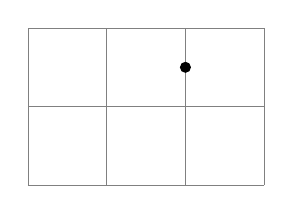
\begin{tikzpicture}
\draw[help lines] (0,0) grid (3,2);
\fill (canvas cs:x=2cm,y=1.5cm) circle (2pt);
\end{tikzpicture}
&
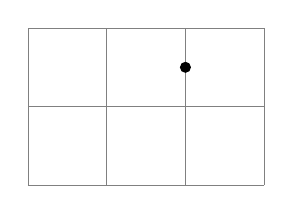
\begin{tikzpicture}
\draw[help lines] (0,0) grid (3,2);
\fill (2,1.5) circle (2pt);
\end{tikzpicture}

\\ \hline  
 \BS{fill} (\RDD{canvas cs}:\blll{x=2cm,y=1.5cm}) circle (2pt);
& \BS{fill} {\color{blue}(2cm,1.5cm)} circle (2pt);
\\ \hline 
\end{tabular} 


\SbSbSSCT{Système de coordonnées polaire \og canvas \fg}{Polar coordinates}

\noindent


\begin{tabular}{|c|c|c|} \hline
\TFRGB{Explicite}{explicit}  & \TFRGB{Implicite}{implicit}
\\ \hline
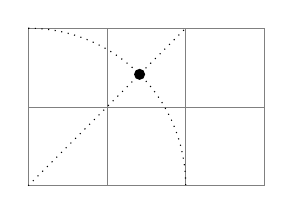
\begin{tikzpicture}
\draw[help lines] (0,0) grid (3,2);
\draw [dotted](0,2) arc (90 :0 :2);
\draw [dotted](0,0) --(2,2);
\fill (canvas polar cs:angle=45,radius=2cm) circle (2pt);
\end{tikzpicture}
&
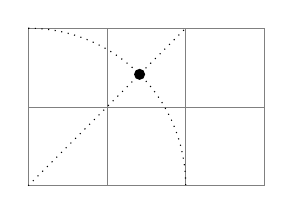
\begin{tikzpicture}
\draw[help lines] (0,0) grid (3,2);
\draw [dotted](0,2) arc (90 :0 :2);
\draw [dotted](0,0) --(2,2);
\fill (45:2cm) circle (2pt);
\end{tikzpicture}
\\ \hline 
\BS{fill} (\RDD{canvas polar cs}:\RDD{angle}=45,\RDD{radius}=2cm) circle (2pt);
&
\BS{fill} {\color{blue}(45:2cm)} circle (2pt);
\\ \hline 
\end{tabular} 

\bigskip
\begin{tabular}{|c|} \hline  
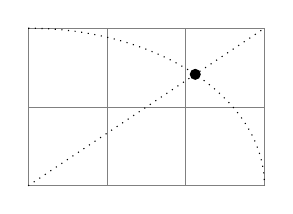
\begin{tikzpicture}
\draw[help lines] (0,0) grid (3,2);
\draw [dotted](0,2) arc (90 :0 :3 and 2);
\draw [dotted](0,0) --(3,2);
\fill (canvas polar cs:angle=45,x radius=3cm,y radius=2cm) circle (2pt);
\end{tikzpicture}
\\ \hline  
\BS{fill} (canvas polar cs:angle=45,\RDD{x radius}=3cm,\RDD{y radius}=2cm) circle (2pt);
\\ \hline 
\end{tabular}


\SbSbSSCT{Système de coordonnées  xyz}{xyz coordinates}

\noindent


\begin{tabular}{|c|c|c|} \hline 
\begin{tikzpicture}[->]
\draw (0,0) -- (xyz cs:x=1);
\draw[red] (0,0) -- (xyz cs:y=1);
\draw[magenta] (0,0) -- (xyz cs:z=1);
\end{tikzpicture}
&
\begin{tikzpicture}[->]
\draw (0,0) -- (1,0,0);
\draw[red]  (0,0) -- (0,1,0);
\draw[magenta]  (0,0) -- (0,0,1);
\end{tikzpicture}
\\ \hline 
\BS{draw} (0,0) - - (\RDD{xyz cs}:x=1); & \BS{draw}  (0,0) - - (1,0,0); \\
\BS{draw}[red]  (0,0) - - (\RDD{xyz cs}:y=1); &  \BS{draw}[red] (0,0) - - (0,1,0); \\
\BS{draw}[magenta]  (0,0) - - (\RDD{xyz cs}:z=1); &  \BS{draw}[magenta]   (0,0) - - (0,0,1); 
\\ \hline 

\end{tabular} 

 
\newpage

\SbSbSSCT{Coordinate system xyz polar}{Coordinate system xyz polar}

\noindent

\begin{tabular}{|c|c|c|} \hline
\TFRGB{Explicite}{explicit}  & \TFRGB{Implicite}{implicit}
\\ \hline
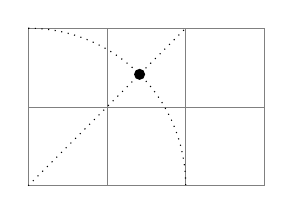
\begin{tikzpicture}
\draw[help lines] (0,0) grid (3,2);
\draw [dotted](0,2) arc (90 :0 :2);
\draw [dotted](0,0) --(2,2);
\fill (xyz polar cs:angle=45,radius=2) circle (2pt);
\end{tikzpicture}
&
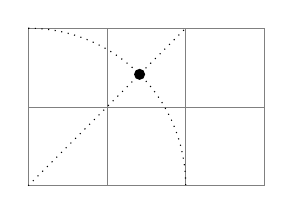
\begin{tikzpicture}
\draw[help lines] (0,0) grid (3,2);
\draw [dotted](0,2) arc (90 :0 :2);
\draw [dotted](0,0) --(2,2);
\fill (45:2) circle (2pt);
\end{tikzpicture}
\\ \hline 
\BS{fill} (\RDD{xyz polar cs}:\RDD{angle}=45,\RDD{radius}=2) circle (2pt);
&
\BS{fill} {\color{blue}(45:2cm)} circle (2pt);
\\ \hline 
\end{tabular} 

\bigskip
\begin{tabular}{|c|} \hline  
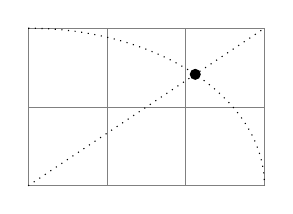
\begin{tikzpicture}
\draw[help lines] (0,0) grid (3,2);
\draw [dotted](0,2) arc (90 :0 :3 and 2);
\draw [dotted](0,0) --(3,2);
\fill (xyz polar cs:angle=45,x radius=3,y radius=2) circle (2pt);
\end{tikzpicture}
\\ \hline  
\BS{fill} (xyz polar cs:angle=45,\RDD{x radius}=3,\RDD{y radius}=2) circle (2pt);
\\ \hline 
\end{tabular} 

\bigskip

\begin{tabular}{|c|c|c|} \hline
\multicolumn{2}{|c|}{\BS{begin}\AC{tikzpicture}{\color{red}[x=1.5cm,y=1cm]} }
\\ \hline
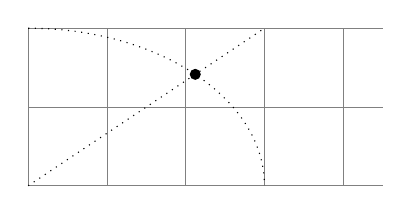
\begin{tikzpicture}[x=1.5cm,y=1cm]
\draw[help lines] (0,0) grid (3,2);
\draw [dotted](0,2) arc (90 :0 :2);
\draw [dotted](0,0) --(2,2);
\fill (xyz polar cs:angle=45,radius=2) circle (2pt);
\end{tikzpicture}
&
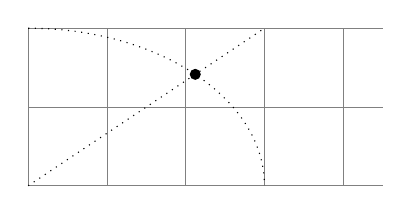
\begin{tikzpicture}[x=1.5cm,y=1cm]
\draw[help lines] (0,0) grid (3,2);
\draw [dotted](0,2) arc (90 :0 :2);
\draw [dotted](0,0) --(2,2);
\fill (45:2) circle (2pt);
\end{tikzpicture}
\\ \hline 
\BS{fill} (\RDD{xyz polar cs}:\RDD{angle}=45,\RDD{radius}=2) circle (2pt);
&
\BS{fill} {\color{blue}(45:2cm)} circle (2pt);
\\ \hline 
\end{tabular} 
\bigskip

\begin{tabular}{|c|c|c|} \hline
\multicolumn{2}{|c|}{\BS{begin}\AC{tikzpicture}{\color{red}[x=\AC{(0cm,1cm)},y=\AC{(-1cm,0cm)}]} }
\\ \hline
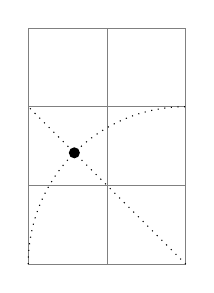
\begin{tikzpicture}[x={(0cm,1cm)},y={(-1cm,0cm)}]
\draw[help lines] (0,0) grid (3,2);
\draw [dotted](0,2) arc (90 :0 :2);
\draw [dotted](0,0) --(2,2);
\fill (xyz polar cs:angle=45,radius=2) circle (2pt);
\end{tikzpicture}
&
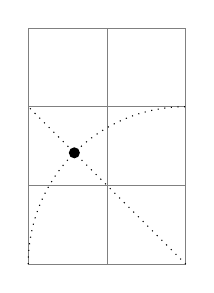
\begin{tikzpicture}[x={(0cm,1cm)},y={(-1cm,0cm)}]
\draw[help lines] (0,0) grid (3,2);
\draw [dotted](0,2) arc (90 :0 :2);
\draw [dotted](0,0) --(2,2);
\fill (45:2) circle (2pt);
\end{tikzpicture}
\\ \hline 
\BS{fill} (\RDD{xyz polar cs}:\RDD{angle}=45,\RDD{radius}=2) circle (2pt);
&
\BS{fill} {\color{blue}(45:2cm)} circle (2pt);
\\ \hline 
\end{tabular} 

\SbSbSSCT{Coordonnées barycentriques}{Barycentric coordinates}

\begin{center}
\RRR{13-2-2}
\end{center}

\begin{tabular}{|c|c|c|} \hline
\multicolumn{3}{|c|}{  \BS{node} [circle,fill=red!20] at (\RDD{barycentric cs}:A=0.6,B=0.3 ) \AC{X};   }\\ 
\hline
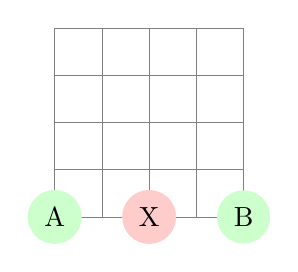
\begin{tikzpicture}[scale=.6]
\draw[help lines] (0,0) grid (4,4);
\node[circle,fill=green!20,] (A) at (0,0) {A};
\node[circle,fill=green!20,] (B) at (4,0) {B};
\node[circle,fill=red!20] at (barycentric cs:A=0.3,B=0.3 ) {X};
\end{tikzpicture}
&
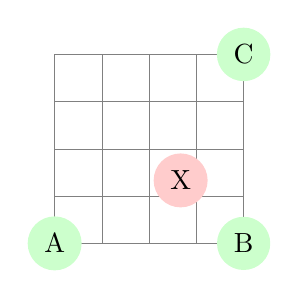
\begin{tikzpicture}[scale=.6]
\draw[help lines] (0,0) grid (4,4);
\node[circle,fill=green!20,] (A) at (0,0) {A};
\node[circle,fill=green!20,] (B) at (4,0) {B};
\node[circle,fill=green!20,] (C) at (4,4) {C};
\node[circle,fill=red!20] at (barycentric cs:A=0.4,B=0.4 ,C=.4) {X};
\end{tikzpicture}
&
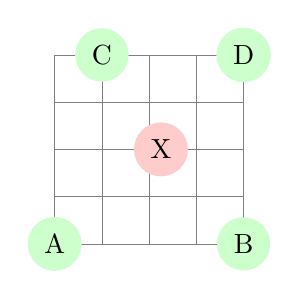
\begin{tikzpicture}[scale=.6]
\draw[help lines] (0,0) grid (4,4);
\node[circle,fill=green!20,] (A) at (0,0) {A};
\node[circle,fill=green!20,] (B) at (4,0) {B};
\node[circle,fill=green!20,] (C) at (1,4) {C};
\node[circle,fill=green!20,] (D) at (4,4) {D};
\node[circle,fill=red!20] at (barycentric cs:A=0.5,B=0.5,C=.5,D=.5 ) {X};
\end{tikzpicture}
\\ \hline
A=0.3,B=0.3 & A=0.4,B=0.4 ,C=.4 & A=0.5,B=0.5,C=.5,D=.5 
\\ \hline
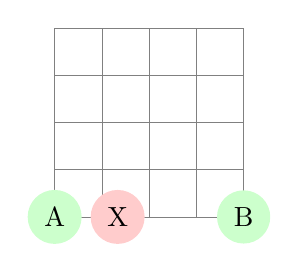
\begin{tikzpicture}[scale=.6]
\draw[help lines] (0,0) grid (4,4);
\node[circle,fill=green!20,] (A) at (0,0) {A};
\node[circle,fill=green!20,] (B) at (4,0) {B};
\node[circle,fill=red!20] at (barycentric cs:A=0.6,B=0.3 ) {X};
\end{tikzpicture}
&
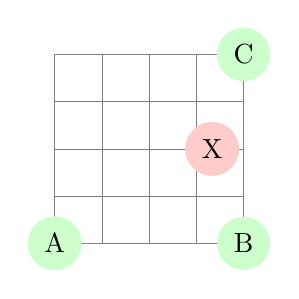
\begin{tikzpicture}[scale=.6]
\draw[help lines] (0,0) grid (4,4);
\node[circle,fill=green!20,] (A) at (0,0) {A};
\node[circle,fill=green!20,] (B) at (4,0) {B};
\node[circle,fill=green!20,] (C) at (4,4) {C};
\node[circle,fill=red!20] at (barycentric cs:A=0.2,B=0.4 ,C=.6) {X};
\end{tikzpicture}
&
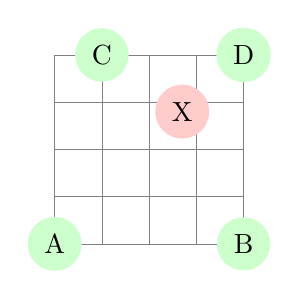
\begin{tikzpicture}[scale=.6]
\draw[help lines] (0,0) grid (4,4);
\node[circle,fill=green!20,] (A) at (0,0) {A};
\node[circle,fill=green!20,] (B) at (4,0) {B};
\node[circle,fill=green!20,] (C) at (1,4) {C};
\node[circle,fill=green!20,] (D) at (4,4) {D};
\node[circle,fill=red!20] at (barycentric cs:A=0.2,B=0.4,C=.6,D=.8 ) {X};
\end{tikzpicture}
\\ \hline
A=0.6,B=0.3 & A=0.2,B=0.4 ,C=.6 & A=0.2,B=0.4,C=.6,D=.8
\\ \hline
\end{tabular}

\SbSbSSCT{Coordonnées nominatives : n\oe ud}{Named coordinates: nodes}

\begin{center}
\RRR{13-2-3}
\end{center}

\begin{tabular}{|c|c|} \hline  
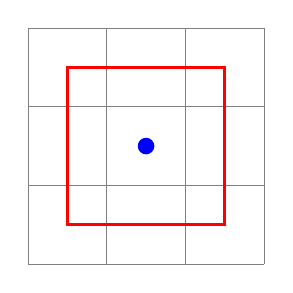
\begin{tikzpicture}[blue,very thick,baseline=1cm]
\draw[help lines] (0,0) grid (3,3);
\coordinate (centre) at (1.5,1.5) ;
\coordinate (A) at (.5,.5) ;
\coordinate (B) at (2.5,2.5) ;
\fill (centre) circle (3pt);
\draw[red] (A) rectangle (B) ;
\end{tikzpicture}
&  
\parbox[c]{8cm}{
\BSS{coordinate} {\color{blue}(centre)} at(1.5,1.5) ; \\
\BSS{coordinate} {\color{blue}(A)} at (.5,.5) ;\\
\BSS{coordinate} {\color{blue}(B)} at  (2.5,2.5) ;\\
\\
\BS{fill} {\color{blue}(centre)} circle (3pt);\\
\BS{draw}[red] {\color{blue}(A)} rectangle {\color{blue}(B)} ;\\
}
\\ \hline 
\end{tabular} 


\TFRGB{voir aussi}{see also} page \pageref{noeuds}


\SbSbSSCT{Coordonnées relatives à un noeud}{Coordinates relative to a node}

\noindent

\begin{tabular}{|c|c|c|c|} \hline
\multicolumn{4}{|l|}{  \BS{node} [draw,fill=green!20,] (A) at (1,1) \AC{\BS{huge}  noeud}; }\\ 
\multicolumn{4}{|l|}{  \BS{fill}[red] (\RDD{node cs}:\RDD{name}=A,\RDD{anchor}=south) circle (3pt);   }\\ 
\hline

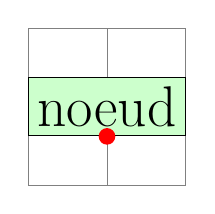
\begin{tikzpicture}
\draw[help lines] (0,0) grid (2,2);
\node[draw,fill=green!20,] (A) at (1,1) {\huge noeud};
\fill[red] (node cs:name=A,anchor=south) circle (3pt);
\end{tikzpicture}
&
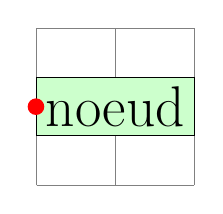
\begin{tikzpicture}
\draw[help lines] (0,0) grid (2,2);
\node[draw,fill=green!20,] (A) at (1,1) {\huge noeud};
\fill[red] (node cs:name=A,anchor=west) circle (3pt);
\end{tikzpicture}
&
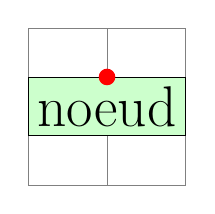
\begin{tikzpicture}
\draw[help lines] (0,0) grid (2,2);
\node[draw,fill=green!20,] (A) at (1,1) {\huge noeud};
\fill[red] (node cs:name=A,anchor=north) circle (3pt);
\end{tikzpicture}
&
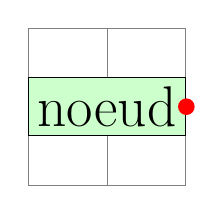
\begin{tikzpicture}
\draw[help lines] (0,0) grid (2,2);
\node[draw,fill=green!20,] (A) at (1,1) {\huge noeud};
\fill[red] (node cs:name=A,anchor=east) circle (3pt);
\end{tikzpicture}
\\ \hline
name=A,anchor=south & name=A,anchor=west & name=A,anchor=north & name=A,anchor=east
\\ \hline
\end{tabular}

\bigskip

\begin{tabular}{|c|c|c|c|} \hline
\multicolumn{4}{|l|}{  \BS{node} [draw,fill=green!20,] \blll{(A)} at (1,1) \AC{\BS{huge}  noeud}; }\\ 
\multicolumn{4}{|l|}{  \BS{fill}[red] (\blll{A}.south) circle (3pt);   }\\ 
\hline

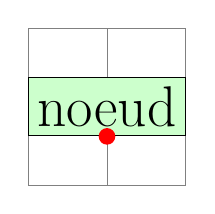
\begin{tikzpicture}
\draw[help lines] (0,0) grid (2,2);
\node[draw,fill=green!20,] (A) at (1,1) {\huge noeud};
\fill[red] (A.south) circle (3pt);
\end{tikzpicture}
&
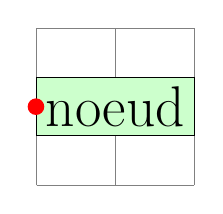
\begin{tikzpicture}
\draw[help lines] (0,0) grid (2,2);
\node[draw,fill=green!20,] (A) at (1,1) {\huge noeud};
\fill[red] (A.west) circle (3pt);
\end{tikzpicture}
&
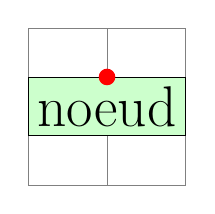
\begin{tikzpicture}
\draw[help lines] (0,0) grid (2,2);
\node[draw,fill=green!20,] (A) at (1,1) {\huge noeud};
\fill[red] (A.north) circle (3pt);
\end{tikzpicture}
&
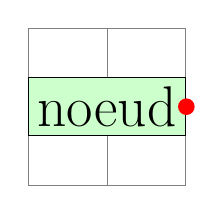
\begin{tikzpicture}
\draw[help lines] (0,0) grid (2,2);
\node[draw,fill=green!20,] (A) at (1,1) {\huge noeud};
\fill[red] (A.east) circle (3pt);
\end{tikzpicture}
\\ \hline
A.south & A.west & A.north & A.east
\\ \hline
\end{tabular}



\bigskip
\begin{tabular}{|c|c|c|c|} \hline
\multicolumn{4}{|c|}{  \BS{fill}[red] (node cs:\RDD{name}=A,\RDD{angle}=0) circle (3pt);  }\\ 
\hline

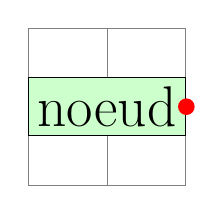
\begin{tikzpicture}
\draw[help lines] (0,0) grid (2,2);
\node[draw,fill=green!20,] (A) at (1,1) {\huge noeud};
\fill[red] (node cs:name=A,angle=0) circle (3pt);
\end{tikzpicture}
&
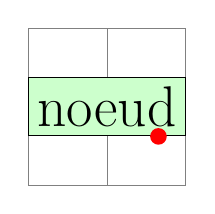
\begin{tikzpicture}
\draw[help lines] (0,0) grid (2,2);
\node[draw,fill=green!20,] (A) at (1,1) {\huge noeud};
\fill[red] (node cs:name=A,angle=-30) circle (3pt);
\end{tikzpicture}
&
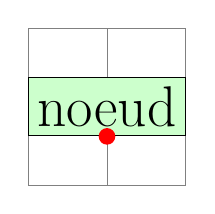
\begin{tikzpicture}
\draw[help lines] (0,0) grid (2,2);
\node[draw,fill=green!20,] (A) at (1,1) {\huge noeud};
\fill[red] (node cs:name=A,angle=-90) circle (3pt);
\end{tikzpicture}
&
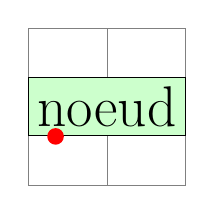
\begin{tikzpicture}
\draw[help lines] (0,0) grid (2,2);
\node[draw,fill=green!20,] (A) at (1,1) {\huge noeud};
\fill[red] (node cs:name=A,angle=-150) circle (3pt);
\end{tikzpicture}
\\ \hline
name=A,angle=0 & name=A,angle=-30 & nname=A,angle=-90 & name=A,angle=-150
\\ \hline
\end{tabular}

\bigskip


\begin{tabular}{|c|c|c|c|} \hline
\multicolumn{4}{|c|}{  \BS{fill}[red] (A.0) circle (3pt);  }\\ 
\hline

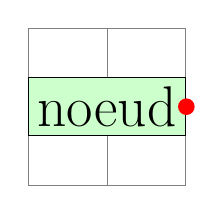
\begin{tikzpicture}
\draw[help lines] (0,0) grid (2,2);
\node[draw,fill=green!20,] (A) at (1,1) {\huge noeud};
\fill[red] (A.0) circle (3pt);
\end{tikzpicture}
&
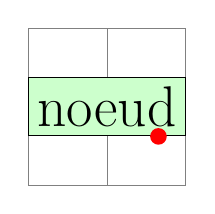
\begin{tikzpicture}
\draw[help lines] (0,0) grid (2,2);
\node[draw,fill=green!20,] (A) at (1,1) {\huge noeud};
\fill[red] (A.-30) circle (3pt);
\end{tikzpicture}
&
\begin{tikzpicture}
\draw[help lines] (0,0) grid (2,2);
\node[draw,fill=green!20,] (A) at (1,1) {\huge noeud};
\fill[red] (A.-90) circle (3pt);
\end{tikzpicture}
&
\begin{tikzpicture}
\draw[help lines] (0,0) grid (2,2);
\node[draw,fill=green!20,] (A) at (1,1) {\huge noeud};
\fill[red] (A.-150) circle (3pt);
\end{tikzpicture}
\\ \hline
A.0 & A.-30 & A.-90 & A.-150
\\ \hline
\end{tabular}

\TFRGB{voir aussi}{see also} page \pageref{nomnoeud}


\newpage

\SbSbSSCT{Coordonnées relatives à deux points}{Coordinates relative to two points}
\begin{center}
\RRR{13-3-1}
\end{center}

\begin{tabular}{|c|c|} \hline
\multicolumn{2}{|c|}{  \BS{node} [circle,fill=red!20] at (1,1 {\color{red}|-} 3,3) \AC{X}   }\\ 
\hline
\begin{tikzpicture}
\draw[help lines] (0,0) grid (4,4);
\node[circle,fill=green!20,] (A) at (1,1) {A};
\node[circle,fill=green!20,] (B) at (3,3) {B};
\node[circle,fill=red!20] at (1,1 |- 3,3) {X};
\end{tikzpicture}
&
\begin{tikzpicture}
\draw[help lines] (0,0) grid (4,4);
\node[circle,fill=green!20,] (A) at (1,1) {A};
\node[circle,fill=green!20,] (B) at (3,3) {B};
\node[circle,fill=red!20] at (1,1 -| 3,3) {X};
\end{tikzpicture}
\\ \hline
at (1,1 {\color{red}|-} 3,3)
&
at (1,1 {\color{red}-|} 3,3)
\\ \hline
\end{tabular}



\SbSbSSCT{Coordonnée relative à une intersection}{Coordinates relative to an intersection}
\begin{center}
\RRR{13-3-2}
\end{center}

 \maboite{\BS{usetikzlibrary}\AC{intersections}}
\label{lib-intersections}


\begin{tabular}{|c|c|c|c|} \hline 
\multicolumn{4}{|l|}{  \BS{draw} [\RDD{name path}=XXX] (2,1) circle  (1cm);   }\\ 
\multicolumn{4}{|l|}{  \BS{draw} [\RDD{name path}=YYY] (0.5,0.5) rectangle +(3,1);   }\\ 
\multicolumn{4}{|l|}{ \BS{fill} [red,\RDD{ name intersections}=\AC{of=xxx and YYY}]
(\RDD{intersection}-1) circle (2pt)   }\\ 
\hline 
\begin{tikzpicture}[scale=.8]
\draw [help lines] grid (4,2);
\draw [name path=XXX] (2,1) circle  (1cm);
\draw [name path=YYY] (0.5,0.5) rectangle +(3,1);
\fill [red, name intersections={of=XXX and YYY}]
(intersection-1) circle (2pt)  ;
\end{tikzpicture}
& 
\begin{tikzpicture}[scale=.8]
\draw [help lines] grid (4,2);
\draw [name path=XXX] (2,1) circle  (1cm);
\draw [name path=YYY] (0.5,0.5) rectangle +(3,1);
\fill [red, name intersections={of=XXX and YYY}] (intersection-2) circle (2pt) ;
\end{tikzpicture} 
&  
\begin{tikzpicture}[scale=.8]
\draw [help lines] grid (4,2);
\draw [name path=XXX] (2,1) circle  (1cm);
\draw [name path=YYY] (0.5,0.5) rectangle +(3,1);
\fill [red, name intersections={of=XXX and YYY}] (intersection-3) circle (2pt) ;
\end{tikzpicture}
&  
\begin{tikzpicture}[scale=.8]
\draw [help lines] grid (4,2);
\draw [name path=XXX] (2,1) circle  (1cm);
\draw [name path=YYY] (0.5,0.5) rectangle +(3,1);
\fill [red, name intersections={of=XXX and YYY}] (intersection-4) circle (2pt) ;
\end{tikzpicture}
\\ 
\hline intersection-1 & intersection-2 &intersection-3  & intersection-4 \\ 
\hline 
\end{tabular} 

\bigskip

\begin{tabular}{|c|} \hline  
\BS{fill} [red, name intersections=\AC{of=XXX and YYY}] \\
(intersection-1) circle (2pt) {\color{red} node[black,above right] \AC{point a}} ;
\\ \hline  
\begin{tikzpicture}
\draw [help lines] grid (4,2);
\draw [name path=XXX] (2,1) circle  (1cm);
\draw [name path=YYY] (0.5,0.5) rectangle +(3,1);
\fill [red, name intersections={of=XXX and YYY}]
(intersection-1) circle (2pt) node[black,above right] {point a} ;
\end{tikzpicture} 
\\ \hline 
\end{tabular} 

\bigskip

\begin{tabular}{|c|} \hline 
\BS{fill} [red, name intersections=\AC{of=XXX and YYY, \RDD{name}=ZZZ}]; \\
\BS{draw} [red] (ZZZ-1) - - (ZZZ-3); \BS{draw} [green] (ZZZ-2) - - (ZZZ-4);
\\ \hline  
\begin{tikzpicture}
\draw [help lines] grid (4,2);
\draw [name path=XXX] (2,1) circle  (1cm);
\draw [name path=YYY] (0.5,0.5) rectangle +(3,1);
\fill [red, name intersections={of=XXX and YYY, name=ZZZ}];
\draw [red] (ZZZ-1) -- (ZZZ-3);
\draw [green] (ZZZ-2) -- (ZZZ-4);
\end{tikzpicture}
\\ \hline 
\end{tabular} 

\bigskip
\begin{tabular}{|c|} \hline  
\BS{fill} [red, name intersections=\AC{of=XXX and YYY , \RDD{by}=\AC{a,b,c,d}}]; \\
\BS{draw} [red] (a) - - (c); \hspace{1cm} \BS{draw} [green] (b) - - (d);
\\ \hline   
\begin{tikzpicture}
\draw [help lines] grid (4,2);
\draw [name path=XXX] (2,1) circle  (1cm);
\draw [name path=YYY] (0.5,0.5) rectangle +(3,1);
\fill [red, name intersections={of=XXX and YYY, by={a,b,c,d}}];
\draw [red] (a) -- (c);
\draw [green] (b) -- (d);
\end{tikzpicture}
\\ \hline 
\end{tabular} 

\bigskip

\begin{tabular}{|c|} \hline  
\BS{fill} [name intersections=\AC{of=XXX and YYY, name=i, \RDD{total}=\BS{t}}] [red] \\
\BS{foreach} \BS{s} in \AC{1,...,\BS{t}} \AC{(i-\BS{s}) circle (2pt) node[black,above right] \AC{\BS{s}}}
\\ \hline  
\begin{tikzpicture}
\draw [help lines] grid (4,2);
\draw [name path=XXX] (2,1) circle  (1cm);
\draw [name path=YYY] (0.5,0.5) rectangle +(3,1);
\fill [name intersections={of=XXX and YYY , name=i, total=\t}]
[red]
\foreach \s in {1,...,\t}{(i-\s) circle (2pt) node[black,above right] {\s}};
\end{tikzpicture}
\\ \hline 
\end{tabular} 



\newpage

\SbSbSSCT{Position calculée avec le module  \og  pgfmath \fg}{Calculated positions with  \og  pgfmath \fg }

\begin{center}
\RRR{13-2-1}
\end{center}

\TFRGB{Ce module est chargé automatiquement avec le module Tikz}{Package automatically loaded with Tikz} 

\begin{tabular}{|c|} \hline 
\begin{tikzpicture}
\draw[help lines] (0,0) grid (4,2);
\fill [red] (canvas cs:x=2cm+1.5cm,y=1.5cm-1cm) circle (3pt);
\fill [blue] (2cm,1.5cm) circle (3pt);
\draw[dashed] (2,1.5) -| (3.5,.5);
\end{tikzpicture}
\\ \hline 
\emph{\TFRGB{Explicite}{explicit}} 
 : \BS{fill} [red] (\RDD{canvas cs}:x=2cm+1.5cm,y=1.5cm-1cm) circle (3pt);
 \\  \hline 
\emph{\TFRGB{Implicite}{implicit}} :  \BS{fill} [red] {\color{red}(2cm+1.5cm,1.5cm-1cm)} circle (3pt);
\\ \hline 
\end{tabular} 

\bigskip
\begin{tabular}{|c|c|c|} \hline 
\begin{tikzpicture}[baseline=0pt]
\draw[help lines] (0,0) grid (4,4);
 \draw[dashed] (2,2) circle (2);
\fill[red](2+ 2*cos 30,2+2*sin 30) circle (3pt);
\fill[magenta](2+ 2*cos{(120)},2+2*sin{(120)}) circle (3pt);
\end{tikzpicture}
&
\parbox[c]{8cm}{
 \BS{draw}[dashed] (2,2) circle (2);\\
 \smallskip
 \BS{fill} [red]{\color{red}(2+ 2*cos 30 , 2+2*sin 30)} circle (3pt);\\
  \smallskip
 \BS{fill}[magenta] {\color{red}(2+2*cos\AC{(120)} , 2+2*sin\AC{(120)})} circle (3pt); 
 }
\\ \hline 
\end{tabular} 

\SbSbSSCT{Position calculée avec \og library calc \fg}{Calculated positions with \og  calc  library calc \fg}

\begin{center}
\RRR{13-5}
\end{center}
\label{lib-calc}

 \maboite{\BS{usetikzlibrary}\AC{calc}}
 
\begin{tabular}{|c|c|} \hline  
\begin{tikzpicture}[baseline=0pt]
\draw [help lines] (0,0) grid (3,2);
\node (a) at (1,1) {A};
\fill [red] ($(a) + 2/3*(1cm,0)$) circle (2pt);
\fill [red] ($(a) + 4/3*(1cm,0)$) circle (2pt);
\end{tikzpicture}
&
\parbox{8cm}{
\BS{node} (a) at (1,1) \AC{A}; \\
\BS{fill} [red] {\color{red} (\$(a) + 2/3*(1cm,0)\$)} circle (2pt); \\
\BS{fill} [red] {\color{red}(\$(a) + 4/3*(1cm,0)\$)} circle (2pt); \\
}
\\ 
\hline 
\end{tabular} 

\SbSbSSCT{Tangentes avec \og library calc \fg}{Tangents with  \og calc library  \fg}

\begin{center}
\RRR{13-2-4}
\end{center}

\begin{tabular}{|c|c|} \hline 
\multicolumn{2}{|l|}{\BS{node}[fill=green!20] (a) at (3,1.5) \AC{A}; } \\
\multicolumn{2}{|l|}{\BS{fill}[red] (\RDD{tangent cs}:\RDD{node}=c,\RDD{point}=\AC{(A)},\RDD{solution}=1);  }\\ 
\hline
\begin{tikzpicture}
\draw[help lines] (0,0) grid (4,2);
\node[fill=green!20] (A) at (3,1.5) {A};
\node [circle,draw] (c) at (1,1) [minimum size=1.5cm] {$c$};
\draw[red,dashed] (A) - -(tangent cs:node=c,point={(A)},solution=1) ;
\draw[red,dashed] (1,1) - -(tangent cs:node=c,point={(3,1.5)},solution=1) ;
\fill[red] (tangent cs:node=c,point={(A)},solution=1) circle (3pt);
\end{tikzpicture}
&
\begin{tikzpicture}
\draw[help lines] (0,0) grid (4,2);
\node[fill=green!20] (A) at (3,1.5) {A};
\node [circle,draw] (c) at (1,1) [minimum size=1.5cm] {$c$};
\draw[red,dashed] (A) - -(tangent cs:node=c,point={(A)},solution=2) ;
\draw[red,dashed] (1,1) - -(tangent cs:node=c,point={(A)},solution=2) ;
\fill[red] (tangent cs:node=c,point={(A)},solution=2) circle (3pt);
\end{tikzpicture}
\\ \hline
\RDD{solution}=1 & \RDD{solution}=2
\\ \hline
\end{tabular} 

\newpage

\SbSbSSCT{Point à pourcentage donné }{Percentage position }

\begin{center}
\RRR{13-5-3}
\end{center}


\begin{tabular}{|c|c|} \hline  
\multicolumn{2}{|c|}{\BS{fill}[red] ({\color{red}\$(0,1)!.25!(4,1)\$}) circle (4pt); } \\  \hline  

\begin{tikzpicture}
\draw [help lines] (0,0) grid (4,2);
\draw [line width= 3pt] (0,1) -- (4,1);
\fill[red] ($(0,1)!.25!(4,1)$) circle (4pt);
\end{tikzpicture}
&  
\begin{tikzpicture}
\draw [help lines] (0,0) grid (4,2);
\draw [line width= 3pt] (0,1) -- (4,1);
\fill[red] ($(0,1)!.75!(4,1)$) circle (4pt);
\end{tikzpicture}
\\ \hline (0,1)!{\color{red}0.25}!(4,1) & (0,1)!{\color{red}0.75}!(4,1) \\ 
\hline 
\end{tabular} 

\bigskip

\begin{tabular}{|c|} \hline  
\begin{tikzpicture}
\draw [help lines] (0,0) grid (4,3);
\draw [line width=2pt ](0,2) -- (4,2);
\draw[red] ($(0,2)!.75!(4,2)$) -- (0,0);
\fill[red] ($(0,2)!.75!(4,2)!.66!(0,0)$) circle (4pt);
\end{tikzpicture}
\\ \hline 
\BS{fill}[red] (\${\color{blue}(0,2)!0.75!(4,2)}!{\color{red}0.66!(0,0)}\$) circle (2pt);
\\ \hline 
\end{tabular} 


\SbSbSSCT{Point à distance donnée}{Position at a given distance }

\begin{center}
\RRR{13-5-4}
\end{center}

\begin{tabular}{|c|c|} \hline  
\multicolumn{2}{|c|}{\BS{fill}[red] ({\color{red}\$(0,1)!1.5cm!(4,1)\$}) circle (4pt); } \\  \hline  

\begin{tikzpicture}
\draw [help lines] (0,0) grid (4,2);
\draw [line width= 2pt] (0,1) -- (4,1);
\fill[red] ($(0,1)!1.5cm!(4,1)$) circle (4pt);
\end{tikzpicture}
&  
\begin{tikzpicture}
\draw [help lines] (0,0) grid (4,2);
\draw [line width= 2pt] (0,1) -- (4,1);
\fill[red] ($(0,1)!3cm!(4,1)$) circle (4pt);
\end{tikzpicture}
\\ \hline (0,1)!{\color{red}1.5cm}!(4,1) & (0,1)!{\color{red}3cm}!(4,1) \\ 
\hline 
\end{tabular} 

\bigskip

\begin{tabular}{|c|} \hline  
\begin{tikzpicture}
\draw [help lines] (0,0) grid (4,4);
\coordinate (a) at (1,0);
\coordinate (b) at (4,1);
\draw [line width= 3pt] (0,0) -- (4,1);
\draw [line width= 2pt,red](2,.5) -- ($ (2,.5)!2cm!90:(4,1) $);
\end{tikzpicture}
\\ \hline
\BS{draw} (2,.05) - - (\$ (2,0.5)!{\color{red}2cm!90:(4,1)} \$);
\\ \hline 
\end{tabular} 

\newpage

\SbSbSSCT{Coordonnées relatives}{Relative coordinates}


\Par{Cartésienne}{Cartesian coordinates}

\begin{center}
\RRR{13-4-1}
\end{center}

\begin{tabular}{|c|c|c|} \hline  
\TFRGB{relative à l'origine}{relative to the origin}  & \TFRGB{relative à une position}{relative to a position}  &  \TFRGB{relative à la dernière position}{relative to the last position}   
\\ \hline  
 
\begin{tikzpicture}
\draw[help lines] (0,-1) grid (3,1); 
 \draw[blue,very thick] (0,0) -- (1,0) - - (2,1) - - (2,-1);
 \fill[red] (0,0) circle (4pt);
\end{tikzpicture}
&
\begin{tikzpicture} %[scale=.8]
\draw[help lines] (0,-1) grid (4,1);
 \draw[blue,very thick] (0,0) - - (1,0) -- +(2,1) -- +(2,-1) ; %–- +(2,-1) ;
 \fill[red] (1,0) circle (4pt);
\end{tikzpicture}
&
\begin{tikzpicture} %[scale=.8]
\draw[help lines] (0,-1) grid (5,1);  
 \draw[blue,very thick] (0,0) -- (1,0)  - - ++(2,1) - - ++(2,-1);
 \fill[red] (1,0) circle (4pt);
 \fill[red] (3,1) circle (4pt);
\end{tikzpicture}
\\ \hline 
\tikz \fill node[fill=green!20,inner sep=0pt]{(0,0)}; - - (1,0) &
 (0,0) - - \tikz \fill node[fill=green!20,inner sep=0pt]{(1,0)};  & (0,0) - - \tikz \fill node[fill=green!20,inner sep=0pt]{(1,0)}; \\
 - - (2,1) - - (2,-1)  &
   - - +(2,1) - - +(2,-1) & - - ++\tikz \fill node[fill=green!20,inner sep=0pt]{(2,1)}; - - ++(2,-1)
\\ \hline 
\end{tabular} 

\bigskip

\begin{tabular}{|c|c|c|} \hline  
\begin{tikzpicture} [scale=.5]
\draw[help lines] (0,-1) grid (6,6);
 \draw[red,dotted,line width=2pt] (0,0) rectangle (2,2) ;
  \draw[green,dotted,line width=2pt] (0,0) rectangle (3,3) ;  
 \draw[blue,line width=2pt] (0,0) rectangle (1,1)  rectangle (2,2) rectangle (3,3);

\end{tikzpicture}

&  
\begin{tikzpicture} [scale=.5]
\draw[help lines] (0,-1) grid (6,6); 
  \draw[green,dotted,line width=2pt] (1,1) rectangle (4,4) ;   
 \draw[blue,line width=2pt] (0,0) rectangle (1,1)  rectangle +(2,2) rectangle +(3,3);
    \fill[red] (1,1) circle (4pt);
\end{tikzpicture}
&  
\begin{tikzpicture} [scale=.5]
\draw[help lines] (0,-1) grid (6,6);  
 \draw[blue,line width=2pt] (0,0) rectangle (1,1)  rectangle ++(2,2) rectangle ++(3,3);
    \fill[red] (1,1) circle (4pt);
     \fill[green] (3,3) circle (4pt); 
\end{tikzpicture}
\\ 
\hline 
\BS{draw} (0,0) rectangle (1,1)   &
\BS{draw} (0,0) rectangle (1,1)   & 
\BS{draw} (0,0) rectangle (1,1)  \\
rectangle (2,2) rectangle (3,3);  &
rectangle +(2,2) rectangle +(3,3);  &
rectangle ++(2,2) rectangle ++(3,3); \\
\hline 
\end{tabular}


\Par{Polaire }{Polar} {}

\bigskip


\noindent

\begin{tabular}{|c|c|c|c|} \hline
\TFRGB{relative à l'origine}{relative to the origin}  & \TFRGB{relative à une position}{relative to a position}  &  \TFRGB{relative à la dernière position}{relative to the last position}   
\\ \hline    
\begin{tikzpicture} %[scale=.8] 
\draw[help lines] (0,-1) grid (3,1);
 \fill[red] (0:0) circle (4pt);
 \draw[blue,very thick] (0:0)-- (0:1) -- (30:2) -- (-30:2);
\end{tikzpicture}
&
\begin{tikzpicture} %[scale=.8] 
\draw[help lines] (0,-1) grid (4,1);
 \fill[red] (1,0) circle (4pt);
 \draw[blue,very thick] (0:0) -- (0:1) -- +(30:2) -- +(-30:2);
\end{tikzpicture}
&
\begin{tikzpicture} %[scale=.8] 
\draw[help lines] (0,-1) grid (5,1);
 \fill[red] (1,0) circle (4pt);
 \fill[red] (2.732,1) circle (4pt);
 \draw[blue,very thick] (0:0)-- (0:1) -- ++(30:2) -- ++(-30:2);
\end{tikzpicture}
\\ \hline
\tikz \fill node[fill=green!20,inner sep=0pt] {(0:0)}; - - (0:1)&
 (0:0) - - \tikz \fill node[fill=green!20,inner sep=0pt] {(0:1)}; & (0:0)- - \tikz \fill node[fill=green!20,inner sep=0pt] {(0:1)}; \\
 - - (30:2) - - (-30:2)  &  - -  +(30:2) - - +(-30:2) & - -  ++\tikz \fill node[fill=green!20,inner sep=0pt] {(30:2)}; - - ++(-30:2)
\\ \hline 
\end{tabular} 

%\subsubsection{coordonnée relative en polaire}
\Par{coordonnée relative en polaire}{Relative polar coordinate}

\begin{center}
\RRR{13-4-2}
\end{center}
\bigskip

\begin{tabular}{|c|c|} \hline 
\multicolumn{2}{|c|}{ \BS{draw}[blue,very thick] (0,0) -- (2,1) -- ([turn]-45:1cm);}
 \\ \hline
\begin{tikzpicture} %[scale=.8] 
\draw[help lines] (0,0) grid (4,2);
 \draw[dotted] (0,0) -- (4,2);
 \draw[blue,very thick] (0,0) -- (2,1) -- ([turn]-45:1cm);
\end{tikzpicture}
&  
\begin{tikzpicture} %[scale=.8] 
\draw[help lines] (0,0) grid (4,2);
 \draw[dotted] (0,0) -- (4,2);
 \draw[blue,very thick] (0,0) -- (2,1) -- ([turn]45:1cm);
\end{tikzpicture}
\\ \hline ([\RDD{turn}]-45:1cm) & ([\RDD{turn}]45:1cm) \\ 
\hline 
\end{tabular}

\bigskip

\begin{tabular}{|c|c|} \hline  
\begin{tikzpicture}  
\draw[help lines] (-1,0) grid (4,3);
\draw [line width=2pt] (4,0) arc (0 :120 :2)  -- ([turn]90:2cm) ;

\end{tikzpicture}
&  
\begin{tikzpicture} %[scale=.8] 
\draw[help lines] (0,0) grid (4,3);
\draw [line width=2pt]  (0,0) to [bend left] (2,2) --  ([turn]0:2cm);
\fill [red](2,2) circle (4pt);
\end{tikzpicture}
\\ \hline  
\BS{draw} (4,0) arc (0 :120 :2)  - - ([\RDD{turn}]90:2cm) ;
& \BS{draw}  (0,0) to [bend left] (2,2) - -  ([\RDD{turn}]0:2cm); \\

\hline 
\end{tabular} 


%\bigskip 
%
%
%\tikz [delta angle=30, radius=1cm]
%\draw (0,0) arc [start angle=0] -- ([turn]0:1cm)
%arc [start angle=30] -- ([turn]0:1cm)
%arc [start angle=60] -- ([turn]30:1cm);



\bigskip

\begin{tabular}{|c|c|c|} \hline  
\multicolumn{3}{|c|}{ \BS{draw}(1,2)
.. controls ([turn]0:2cm) .. ([turn]-90:2cm); }
\\ \hline
\begin{tikzpicture} %[scale=.8] 
\draw[help lines] (0,0) grid (4,4);
 \draw [line width=2pt] (1,2)
.. controls ([turn]0:2cm) .. ([turn]-90:2cm);
\end{tikzpicture}
&  
\begin{tikzpicture} %[scale=.8] 
\draw[help lines] (0,0) grid (4,4);
 \draw [line width=2pt] (1,2)
.. controls ([turn]30:2cm) .. ([turn]-90:2cm);
\end{tikzpicture}
&  
\begin{tikzpicture} %[scale=.8] 
\draw[help lines] (-2,0) grid (2,4);
 \draw [line width=2pt] (1,2)
.. controls ([turn]0:2cm) .. ([turn]90:2cm);

\end{tikzpicture}
\\ \hline ([turn]0:2cm) .. ([turn]-90:2cm) & ([turn]30:2cm) .. ([turn]-90:2cm) & ([turn]0:2cm) .. ([turn]90:2cm) \\ 
\hline 
\end{tabular} 


\tikzset{every picture/.style=blue,very thick,inner sep=.3333em}

%
%
%
%\newpage
%
%\SSCT{Les n\oe uds }{Nodes}
%
%\SbSSCT{Définition des  n\oe uds}{Creation of nodes}
\tikzset{blue}

\label{noeuds}
\noindent

\begin{tabular}{|c | c | c | c | c |} \hline
\multicolumn{5}{|c|}{  \BS{draw} (1,1) node[\RDD{fill}=red!20] \AC{};   }\\ 
\hline 
\tikz \draw (0,0) grid (2,2) (1,1) node[fill=red!20] {};
&
\tikz \draw (0,0) grid (2,2) (1,1) node[fill=red!20,draw] {}; 
&
\tikz \draw (0,0) grid (2,2) (1,1) node[circle,fill=red!20] {};
&
\tikz \draw (0,0) grid (2,2) (1,1) node[circle,fill=red!20,draw] {};
&
\tikz \draw (0,0) grid (2,2) (1,1) node[coordinate] {};
\\  \hline
\dft
&
node[\RDD{draw}] 
&
 node[\RDD{circle}]  
&
 node[\RDD{circle},\RDD{draw}]
 &
  node[\RDD{coordinate}]
 \\  \hline
\end{tabular}
\bigskip

\begin{tabular}{|c | c | c | c | } \hline
\multicolumn{4}{|c|}{ \BSS{node} \RDD{at} (1,1) [fill=red!20] \AC{};   }\\ 
\hline 
 \begin{tikzpicture}
\draw (0,0) grid (2,2) ; 
\node at (1,1) [fill=red!20] {};
 \end{tikzpicture}
&
 \begin{tikzpicture}
\draw (0,0) grid (2,2) ; 
\node at (1,1) [draw] {};
 \end{tikzpicture}
&
 \begin{tikzpicture}
\draw (0,0) grid (2,2) ; 
\node at (1,1) [fill=red!20,circle] {};
 \end{tikzpicture}
&
 \begin{tikzpicture}
\draw (0,0) grid (2,2) ; 
\node at (1,1) [circle,draw] {};
 \end{tikzpicture}

\\  \hline
[fill=red!20]
&
[\RDD{draw}] 
&
[\RDD{circle},fill=red!20]
 &
[\RDD{circle},draw] 
 \\  \hline
\end{tabular}
\bigskip

\TFRGB{Autres types de n\oe uds voir page}{Other type of nodes see page} \pageref{noeudboite}
\bigskip


\begin{tabular}{|c|c|} \hline 
\BS{draw} (0,0) node at (1,0) \AC{1} node at (2,0) \AC{2} & \BS{draw}(0,0) node foreach \BS{x} in \AC{1,2,...,5}\\ 
node at (3,0) \AC{3} node at (4,0) \AC{4} node at (5,0) \AC{5}; &  at (\BS{x},0) \AC{\BS{x}};\\ 
\hline 
\tikz \draw (0,0) node at (1,0) {1} node at (2,0) {2} node at (3,0) {3} node at (4,0) {4} node at (5,0) {5};
&
\tikz \draw (0,0) node foreach \x in {1,2,...,5} at (\x,0) {\x};
\\ \hline 
\end{tabular} 



\bigskip

\begin{tabular}{|c|} \hline 
\BS{draw}[\rouge{every node/.style=\AC{draw,red}}](0,0) node foreach \BS{x} in \AC{1,2,...,5} at (\BS{x},0) \AC{\BS{x}};
\\ \hline 
\rule[-3pt]{0pt}{.8cm}\tikz \draw[every node/.style={draw,red}] (0,0) node foreach \x in {1,2,...,5} at (\x,0) {\x};
\\ \hline 
\end{tabular} 

\bigskip

\begin{tabular}{|c|} \hline 
\BS{draw}[\rouge{every rectangle node/.style=\AC{draw,red}},\\
\rouge{every circle node/.style=\AC{draw,double}}]\\ (0,0) node at (1,0) \AC{1} node[circle] at (2,0) \AC{2} \\ node[circle] at (3,0) \AC{3} node at (4,0) \AC{4} node at (5,0) \AC{5};
\\ \hline 
\rule[-3pt]{0pt}{1cm} \tikz \draw[every rectangle node/.style={draw,red},
every circle node/.style={draw,double}] (0,0) node at (1,0) {1} node[circle] at (2,0) {2} node[circle] at (3,0) {3} node at (4,0) {4} node at (5,0) {5};
\\ \hline 
\end{tabular} 

\SbSSCT{Nom des  n\oe uds}{Node name}


\begin{tabular}{|c|c|c|}
\hline 
\multicolumn{3}{|c|}{} \\ 
\hline 
\begin{tikzpicture}
\node[name=A,fill=red] at (0,0) {};
\draw  (-1,-1) grid (1,1) ;
\draw (A) circle (.5) ;
\end{tikzpicture} 
&  
\begin{tikzpicture}
\node[name=A,alias=B,fill=red] at (0,0) {} ;
\draw  (-1,-1) grid (1,1) ;
\draw (B) circle (.5) ;
\end{tikzpicture}
& 
\begin{tikzpicture}
\node[fill=red] (C) at (0,0) {};
\draw  (-1,-1) grid  (1,1) ;
\draw (C) circle (.5);
\end{tikzpicture} \\ 
\hline 
\BS{node}[\RDD{name}=A] at (0,0) \AC{}  & \BS{node}[\RDD{name}=A,\RDD{alias}=B] at (0,0) \AC{}  & 
\BS{node}\rouge {(C)} at (0,0) \AC{} \\ 
\BS{draw} (A) circle (.5); & \BS{draw}  (B) circle (.5); &\BS{draw} (C) circle (.5);
\\ \hline 
\end{tabular} 
\newpage

\SbSSCT{Contenu des  n\oe uds}{Node contents}
\tikzset{blue}

\begin{center}
\RRR{17-2-1}
\end{center}

\begin{tabular}{|c|c|} \hline 
\BS{node} at (1,1) [fill=red!20]\rouge { \AC{XXX} };
&  
\BS{node} at (1,1) [fill=red!20,\RDD{node contents}=XXX] \AC{};
\\  \hline 
 \begin{tikzpicture}
\draw (0,0) grid (2,2) ; 
\node at (1,1) [fill=red!20] {XXX};
\end{tikzpicture}
&  
\begin{tikzpicture}
\draw (0,0) grid (2,2) ; 
\node at (1,1) [fill=red!20,node contents=XXX] {};
\end{tikzpicture} 
\\ \hline 
\end{tabular} 

\bigskip

\begin{tabular}{|c|c|} \hline 
\BS{node}[red] at (1,1) [fill=blue!20] \AC{XXX} ;
&  
\BS{node}[red] at (1,1) [fill=blue20,node contents=XXX] \AC{};
\\  \hline 
 \begin{tikzpicture}
\draw (0,0) grid (2,2) ; 
\node[red] at (1,1) [fill=blue!20] {XXX};
\end{tikzpicture}
&  
\begin{tikzpicture}
\draw (0,0) grid (2,2) ; 
\node[red] at (1,1) [fill=blue!20,node contents=XXX] {};
\end{tikzpicture} 
\\ \hline 
\end{tabular} 


\SbSSCT{Premier ou arrière plan}{Behind or in front}

\begin{tabular}{|c|c|} \hline 
\multicolumn{2}{|l|}{\BS{tikz} \BS{fill} [fill=blue!50, draw=blue, very thick]
(0,0) } \\ 
\multicolumn{2}{|l|}{node [\RDD{behind path}, fill=red!50] \AC{XXXXX} }  \\
\multicolumn{2}{|l|}{- - (1.5,0) - - (1.5,1) - - (0,1) ;}
\\ \hline 
\tikz \fill [fill=blue!50, draw=blue, very thick]
(0,0) node [behind path, fill=red!50] {XXXXX}
-- (1.5,0) 
-- (1.5,1) 
-- (0,1) ;
&  
\tikz \fill [fill=blue!50, draw=blue, very thick]
(0,0) node [in front of path, fill=red!50] {XXXXX}
-- (1.5,0) 
-- (1.5,1) 
-- (0,1) ;
\\ \hline 
\RDD{behind path}
&  
\RDD{in front of path}
\\ \hline 
\end{tabular}



\SbSSCT{Noms à préfixe ou suffixe}{Name prefix or name suffix}


\begin{tabular}{|c|c|}
\hline 
\begin{tikzpicture}[every node/.style={draw},baseline=0pt]
\draw[name prefix = top-] node (A) at (1,1) {A} node (B) at (2,1) {B} node (C) at (3,1) {C};
\draw[name prefix = bottom-] node (1) at (1,0) {1} node (2) at (2,0) {2} node(3) at  (3,0) {3};
\draw [red] (top-A) -- (bottom-3);
\end{tikzpicture} 
&
\parbox{12cm}{
\BS{draw}[\RDD{name prefix} = \blll{top-} ] node (A) at (1,1) \AC{A} node (B) at (2,1) \AC{B} node (C) at (3,1) \AC{C}; \\
\BS{draw}[\RDD{name prefix} = \blll{bottom-}] node (1) at (1,0) \AC{1} node (2) at (2,0) \AC{2} node(3) at  (3,0) \AC{3}; \\
\BS{draw} [red] (\blll{top-}A) -- (\blll{bottom-}3);}
\\ \hline
\begin{tikzpicture}[every node/.style={draw},baseline=0pt]
\draw[name suffix= -top] node (A) at (1,1) {A} node (B) at (2,1) {B} node (C) at (3,1) {C};
\draw[name suffix=  -bottom] node (1) at (1,0) {1} node (2) at (2,0) {2} node(3) at  (3,0) {3};
\draw [red] (A-top) -- (3-bottom);
\end{tikzpicture}
&
\parbox{12cm}{
\BS{draw}[\RDD{name suffix} = \blll{-top}] node (A) at (1,1) \AC{A} node (B) at (2,1) \AC{B} node (C) at (3,1) \AC{C}; \\
\BS{draw}[\RDD{name suffix} = \blll{-bottom}] node (1) at (1,0) \AC{1} node (2) at (2,0) \AC{2} node(3) at  (3,0) \AC{3}; \\
\BS{draw} [red] (A \blll{-top}) - - (3 \blll{-bottom});}
\\ \hline 

\end{tabular} 


\SbSSCT{Liaisons}{Links}
\label{liaisons}

\begin{tabular}{|c|c|c|} \hline 
\multicolumn{3}{|l|}{\BS{node}[draw] (A) at (0,0) \AC{A}; \hspace{.5cm} \BS{node}[draw] (B) at (1.5,1.5) \AC{B}; \hspace{.5cm} \BS{draw} (A) - - (B) } \\ \hline 
\begin{tikzpicture}[blue]
\node[draw] (A) at (0,0) {A};
\node[draw] (B) at (1.5,1.5) {B};
\draw (A) -- (B);
\end{tikzpicture}
&  
\begin{tikzpicture}[blue]
\node[draw] (A) at (0,0) {A};
\node[draw] (B) at (1.5,1.5) {B};
\draw (A) |- (B);
\end{tikzpicture}
&  
\begin{tikzpicture}[blue]
\node[draw] (A) at (0,0) {A};
\node[draw] (B) at (1.5,1.5) {B};
\draw (A) -| (B);
\end{tikzpicture}
\\ \hline  
(A){\color{red} - -} (B) & (A) {\color{red}|-} (B) &  (A) {\color{red}-|} (B)
\\ \hline 
\begin{tikzpicture}[blue]
\node[draw] (A) at (0,0) {A};
\node[draw] (B) at (1.5,1.5) {B};
\draw (A) to [bend right] (B);
\end{tikzpicture}
&  
\begin{tikzpicture}[blue]
\node[draw] (A) at (0,0) {A};
\node[draw] (B) at (1.5,1.5) {B};
\draw (A) to [bend left] (B);
\end{tikzpicture}
&  
\begin{tikzpicture}[blue]
\node[draw] (A) at (0,0) {A};
\node[draw] (B) at (1.5,1.5) {B};
\draw (A) to[bend left=0] (B);
\end{tikzpicture}
\\ \hline  
(A) to [\RDD{bend right}] (B) & (A) to [\RDD{bend left}] (B) &  (A) to[\RDD{bend left}=0] (B)
\\ \hline 
\begin{tikzpicture}[blue]
\node[draw] (A) at (0,0) {A};
\node[draw] (B) at (1.5,1.5) {B};
\draw (A) to[bend left=120]  (B);
\end{tikzpicture}
&  
\begin{tikzpicture}[blue]
\node[draw] (A) at (0,0) {A};
\node[draw] (B) at (1.5,1.5) {B};
\draw (A) to[bend left=45] (B);
\end{tikzpicture}
&  
\begin{tikzpicture}[blue]
\node[draw] (A) at (0,0) {A};
\node[draw] (B) at (1.5,1.5) {B};
\draw (A) to[bend left=90] (B);
\end{tikzpicture}
\\ \hline  
(A)  to[\RDD{bend left}=120]  (B) & (A) to[\RDD{bend left}=45] (B) &  (A) to[\RDD{bend left}=90] (B)
\\ \hline 
\begin{tikzpicture}[blue]
\node[draw] (A) at (0,0) {A};
\node[draw] (B) at (1.5,1.5) {B};
\draw (A)  to[out=90]  (B);
\end{tikzpicture}
&  
\begin{tikzpicture}[blue]
\node[draw] (A) at (0,0) {A};
\node[draw] (B) at (1.5,1.5) {B};
\draw (A) to[out=30] (B);
\end{tikzpicture}
&  
\begin{tikzpicture}[blue]
\node[draw] (A) at (0,0) {A};
\node[draw] (B) at (1.5,1.5) {B};
\draw (A)  to[in=-90]  (B);
\end{tikzpicture}
\\ \hline  
(A)  to[\RDD{out}=90] (B) & (A) to[\RDD{out}=30]  (B) &  (A)  to[\RDD{in}=-90]  (B)
\\ \hline  
\end{tabular} 

\bigskip
\begin{tabular}{|c|c|c|} \hline  
\multicolumn{2}{|c|}{ \BS{draw} (A) .. controls +(right:2cm) and +(down:2cm) .. (B);  }\\ 
\hline  
\begin{tikzpicture}[blue]
\node[draw] (A) at (0,0) {A};
\node[draw] (B) at (2,2) {B};
\draw  (A) .. controls +(right:2cm) and +(down:2cm) .. (B);
\end{tikzpicture}
&
\begin{tikzpicture}[blue]
\node[draw] (A) at (0,0) {A};
\node[draw] (B) at (2,2) {B};
\draw  (A) .. controls +(up:1cm) and +(left:1cm) .. (B);
\end{tikzpicture}
\\ \hline 
controls +(right:2cm) and +(down:2cm)  &
controls +(up:1cm) and +(left:1cm)
\\ \hline 
\begin{tikzpicture}[blue]
\node[draw] (A) at (0,0) {A};
\node[draw] (B) at (2,2) {B};
\draw  (A) .. controls +(right:1cm) and +(right:2cm) .. (B);
\end{tikzpicture}
&
\begin{tikzpicture}[blue]
\node[draw] (A) at (0,0) {A};
\node[draw] (B) at (2,2) {B};
\draw  (A) .. controls +(up:1cm) and +(right:2cm) .. (B);
\end{tikzpicture}
\\ \hline 
controls +(right:1cm) and +(right:2cm)  &
controls +(up:1cm) and +(right:2cm) 
\\ \hline 
\begin{tikzpicture}[blue]
\node[draw] (A) at (0,0) {A};
\node[draw] (B) at (2,2) {B};
\draw  (A) .. controls +(120:2cm) and +(200:1cm) .. (B);
\end{tikzpicture}
 &
 \begin{tikzpicture}[blue]
 \node[draw] (A) at (0,0) {A};
 \node[draw] (B) at (2,2) {B};T
 \draw  (A) .. controls +(120:2cm) and +(200:1cm) .. (A);
 \end{tikzpicture}
\\  \hline  
controls +(120:2cm) and +(200:1cm) & controls +(120:2cm) and +(200:1cm) 
\\ \hline 
\begin{tikzpicture}[blue]
\node[draw] (A) at (0,0) {A};
\node[draw] (B) at (2,2) {B};
\node[draw] (C) at (0,1) {C};
\node[draw] (D) at (3,0) {D};
\draw  (A) .. controls +(C) and +(D) .. (B);
\end{tikzpicture}
&
\begin{tikzpicture}[blue]
\node[draw] (A) at (0,0) {A};
\node[draw] (B) at (2,2) {B};
\node[draw] (C) at (0,1) {C};
\node[draw] (D) at (3,0) {D};
\draw (A) .. controls +(D)  .. (B);
\end{tikzpicture}
\\ \hline 
controls +(C) and +(D) &
controls +(D) 
\\ \hline 
\end{tabular} 
 \bigskip
 
\begin{tabular}{|c|c|c|} \hline 
\multicolumn{3}{|l|}{ \BS{node}[draw] (A) at (0,0) \AC{A}  }\\

\multicolumn{3}{|l|}{ \BS{node}[draw] (B) at (2,2) \AC{B} \RDD{edge}  [->] (A);  }\\
\multicolumn{3}{|c|}{\RRR{17-12-1}}  \\
\hline 
 \begin{tikzpicture}
 \node[draw] (A) at (0,0) {A};
 \node[draw] (B) at (2,2) {B} edge [->] (A);
 \end{tikzpicture}
 &
 \begin{tikzpicture}
 \node[draw] (A) at (0,0) {A};
 \node[draw] (B) at (2,2) {B} edge [red]  (A);
 \end{tikzpicture}
 &
 \begin{tikzpicture}
 \node[draw] (A) at (0,0) {A};
 \node[draw] (B) at (2,2) {B} edge [dashed] (A);
 \end{tikzpicture}
\\ \hline 
[->] & [red]  & [dashed]
\\ \hline 
\end{tabular}

\SbSSCT{\'Etiquettes sur les n\oe uds}{Node labels}

\begin{tabular}{|c|c|c|c|} \hline
\multicolumn{4}{|c|}{  \BS{fill}(0,0) circle (2pt) node[\RDD{above}] \AC{texte} ; \RRR{17-5-2}   }\\ 
\hline 
  
\begin{tikzpicture} \draw[help lines] (-1,-1) grid (1,1) ;\fill (0,0) circle (2pt) node[above] {texte};\end{tikzpicture}
& 
\begin{tikzpicture} \draw[help lines] (-1,-1) grid (1,1) ;\fill (0,0) circle (2pt) node[below] {texte};\end{tikzpicture}
 &  
\begin{tikzpicture} \draw[help lines] (-1,-1) grid (1,1);\fill (0,0) circle (2pt) node[left] {texte};\end{tikzpicture}
 &  
\begin{tikzpicture} \draw[help lines] (-1,-1) grid (1,1); \fill (0,0) circle (2pt) node[right] {texte};\end{tikzpicture}
 \\  \hline 
 [\RDD{above}] & [\RDD{below}] & [\RDD{left}] &  [\RDD{right}]
 \\ \hline 
 \begin{tikzpicture} \draw[help lines] (-1,-1) grid (1,1) ;\fill (0,0) circle (2pt) node[above left] {texte};\end{tikzpicture}
 & 
 \begin{tikzpicture} \draw[help lines] (-1,-1) grid (1,1) ;\fill (0,0) circle (2pt) node[below left] {texte};\end{tikzpicture}
  &  
 \begin{tikzpicture} \draw[help lines] (-1,-1) grid (1,1);\fill (0,0) circle (2pt) node[above right] {texte};\end{tikzpicture}
  &  
 \begin{tikzpicture} \draw[help lines] (-1,-1) grid (1,1); \fill (0,0) circle (2pt) node[below right] {texte};\end{tikzpicture}
  \\  \hline 
  [\RDD{above left}] & [\RDD{below left}] & [\RDD{above right}] &  [\RDD{below right}]
  \\ \hline 
 \begin{tikzpicture} \draw[help lines] (-1,-1) grid (1,1) ;\fill (0,0) circle (2pt) node[anchor=south] {texte};\end{tikzpicture}
 & 
 \begin{tikzpicture} \draw[help lines] (-1,-1) grid (1,1) ;\fill (0,0) circle (2pt) node[anchor=west] {texte};\end{tikzpicture}
  &  
 \begin{tikzpicture} \draw[help lines] (-1,-1) grid (1,1);\fill (0,0) circle (2pt) node[anchor=north] {texte};\end{tikzpicture}
  &  
 \begin{tikzpicture} \draw[help lines] (-1,-1) grid (1,1); \fill (0,0) circle (2pt) node[anchor=east] {texte};\end{tikzpicture}
  \\  \hline 
  [\RDD{anchor}=south] & [\RDD{anchor}=west] & [\RDD{anchor}=north] & [\RDD{anchor}=east]                                                                                                                                                               ]
  \\ \hline 
 \begin{tikzpicture} \draw[help lines] (-1,-1) grid (1,1) ;\fill (0,0) circle (2pt) node[anchor=south east] {texte};\end{tikzpicture}
 & 
\begin{tikzpicture} \draw[help lines] (-1,-1) grid (1,1) ;\fill (0,0) circle (2pt) node[anchor=south west] {texte};\end{tikzpicture}
&  
\begin{tikzpicture} \draw[help lines] (-1,-1) grid (1,1);\fill (0,0) circle (2pt) node[anchor=north west] {texte};\end{tikzpicture}
&  
\begin{tikzpicture} \draw[help lines] (-1,-1) grid (1,1); \fill (0,0) circle (2pt) node[anchor=east] {texte};\end{tikzpicture}
\\  \hline 
[\RDD{anchor}=south east] & [\RDD{anchor}=south west] & [\RDD{anchor}=north west] & [\RDD{anchor==north east                                                                                                                                                       }]
  \\ \hline 
\end{tabular} 


\bigskip
\begin{tabular}{|c|c|c|c|} \hline
\multicolumn{4}{|c|}{  \BS{fill}(0,0) circle (2pt) node[\RDD{above}=.3cm] \AC{texte} ; \RRR{17-5-2}  }\\ 
\hline 
  
\begin{tikzpicture} \draw[help lines] (-1,-1) grid (1,1) ;\fill (0,0) circle (2pt) node[above=.3cm] {texte};\end{tikzpicture}
& 
\begin{tikzpicture} \draw[help lines] (-1,-1) grid (1,1) ;\fill (0,0) circle (2pt) node[below=.3cm] {texte};\end{tikzpicture}
 &  
\begin{tikzpicture} \draw[help lines] (-1,-1) grid (1,1);\fill (0,0) circle (2pt) node[left=.3cm] {texte};\end{tikzpicture}
 &  
\begin{tikzpicture} \draw[help lines] (-1,-1) grid (1,1); \fill (0,0) circle (2pt) node[right=.3cm] {texte};\end{tikzpicture}
 \\  \hline 
 [\RDD{above}=.3cm] & [\RDD{below}=.3cm] & [\RDD{left}=.3cm] &  [\RDD{right}=.3cm]]
 \\ \hline 
\begin{tikzpicture} \draw[help lines] (-1,-1) grid (1,1) ;\fill (0,0) circle (2pt) node[above left=.3cm] {texte};\end{tikzpicture}
& 
\begin{tikzpicture} \draw[help lines] (-1,-1) grid (1,1) ;\fill (0,0) circle (2pt) node[below left=.3cm] {texte};\end{tikzpicture}
 &  
\begin{tikzpicture} \draw[help lines] (-1,-1) grid (1,1);\fill (0,0) circle (2pt) node[above right=.3cm] {texte};\end{tikzpicture}
 &  
\begin{tikzpicture} \draw[help lines] (-1,-1) grid (1,1); \fill (0,0) circle (2pt) node[below right=.3cm] {texte};\end{tikzpicture}
 \\  \hline 
 [\RDD{above left}=.3cm] & [\RDD{below left}=.3cm] & [\RDD{above right}=.3cm] &  [\RDD{below right}=.3cm]]
 \\ \hline 
 
 \end{tabular} 

 
 \newpage
\selectlanguage{french}
 
 \begin{tabular}{|c|c|c|c|c|} \hline
 \multicolumn{5}{|l|}{ \BSS{shorthandoff}\AC{:} \footnotemark[1]  } \\
 \multicolumn{5}{|l|}{  \BS{node} [draw,\RDD{label}=right:texte] \AC{}   }\\
 \multicolumn{5}{|l|}{ \BSS{shorthandon}\AC{:} } \\ 
 \hline 
     \shorthandoff{:} 
 \tikz \node [draw,label=right:texte] {};
 \shorthandon{:}
 &
  \shorthandoff{:}
 \tikz \node [draw,label=left:texte] {};
 \shorthandon{:}
 &
  \shorthandoff{:}
 \tikz \node [draw,label=above:texte] {};
 \shorthandon{:}
 &
  \shorthandoff{:}
 \tikz \node [draw,label=below:texte] {};
 \shorthandon{:}
 &
  \shorthandoff{:}
 \tikz \node [draw,label=45:texte] {};
    \shorthandon{:}
   \\ \hline
  label=right & label=left &  label=above & label=below & label=45
    \\ \hline 
 \end{tabular}
 \footnotetext[1]{\TFRGB{désactivation et ré-activation de \og : \fg  conflit entre les modules Tikz et Babel en français}{Only useful when the package babel is loaded with the frenchb option    }}
 
 \bigskip
  \begin{tabular}{|c|c|c|c|c|} \hline
  \BS{fill}(0,0) circle (2pt) node[below right=.3cm,draw,label=45:étiquette] \AC{texte} ;
      \\ \hline 
  
  \shorthandoff{:}
\begin{tikzpicture} \draw[help lines] (-1,-1) grid (2,1); \fill (0,0) circle (2pt) node[below right=.3cm,draw,label=45:étiquette] {texte};\end{tikzpicture}
 \shorthandon{:}
 
    \\ \hline 
 \end{tabular}
\bigskip

 \shorthandoff{:}

\SbSSCT{\'Etiquettes épinglées}{The Pin Option} 

\begin{center}
\RRR{17-10-3}
\end{center}
 
\begin{tabular}{|c|c|c|} \hline
\multicolumn{3}{|c|}{  \BSS{shorthandoff}\AC{:} \BS{node}[circle,draw,blue,\RDD{pin}=texte] \AC{} ;   \BSS{shorthandon}\AC{:}  \footnotemark[1] }\\ 
\hline
\begin{tikzpicture} 
\node [circle,draw,blue,pin=texte] {};
\end{tikzpicture}
&
\begin{tikzpicture} 
\node [circle,draw,blue,pin=60:texte] {};
\end{tikzpicture}
&
\begin{tikzpicture} 
\node [circle,draw,blue,pin=right:texte] {};
\end{tikzpicture}
 \\ \hline
[circle,pin=texte] &   [circle,pin=60:texte] & [circle,pin=right:texte]
 \\ \hline 
\end{tabular}  

\bigskip
\begin{tabular}{|c|c|c|} \hline
\multicolumn{3}{|c|}{  \BS{tikz}[\RDD{pin position}=60] \BS{node} [circle,pin=texte] \AC{} ;   }\\ 
\hline 
\tikz[pin position=60] \node [circle,draw,blue,pin=texte] {};
&
\tikz[pin distance=0 cm] \node [circle,draw,blue,pin=60:texte] {};
&
\tikz[pin distance=2 cm] \node [circle,draw,blue,pin=60:texte,pin distance=0cm] {};
  \\ \hline
  [\RDD{pin position}=60] & [\RDD{pin distance}=0 cm] & [\RDD{pin distance}=2 cm]
    \\ \hline
  \dft{ : above} & \multicolumn{2}{|c|}{ \dft{ : 3 ex}}
      \\ \hline
\end{tabular}  

\newpage

   \shorthandon{:} 
   
\selectlanguage{english}   

\SbSSCT{ N\oe uds  sur un chemin}{Nodes on a path}

\RRR{17-8}

\begin{tabular}{|c|c|c|} \hline
\multicolumn{3}{|c|}{  \BS{draw}(0,0) .. controls (1,2) and (2,-1) .. (4,0) node[\RDD{at end}] \AC{texte} ;   }\\ 
\hline 
\tikz \draw (0,0) .. controls (1,2) and (2,-1) .. (4,0) node[pos=0] {texte}; 
&
\tikz \draw (0,0) .. controls (1,2) and (2,-1) .. (4,0) node[pos=.33] {texte}; 
&
\tikz \draw (0,0) .. controls (1,2) and (2,-1) .. (4,0) node[at end] {texte}; 
  \\ \hline 
\RDD{pos}{\color{red}  =0} & \RDD{pos}{\color{red}  =.33} & \RDD{at end} (pos=1)
  \\ \hline 

\tikz \draw (0,0) .. controls (1,2) and (2,-1) .. (4,0) node[very near end] {texte}; 
&
\tikz \draw (0,0) .. controls (1,2) and (2,-1) .. (4,0) node[near end] {texte}; 
&
\tikz \draw (0,0) .. controls (1,2) and (2,-1) .. (4,0) node[midway] {texte}; 
  \\ \hline 
\RDD{very near end} (pos=0.875.) & \RDD{ near end} (pos=0.75) & \RDD{midway} (pos=0.5)
  \\ \hline 
  
\tikz \draw (0,0) .. controls (1,2) and (2,-1) .. (4,0) node[near start] {texte}; 
&
\tikz \draw (0,0) .. controls (1,2) and (2,-1) .. (4,0) node[very near start] {texte}; 
&
\tikz \draw (0,0) .. controls (1,2) and (2,-1) .. (4,0) node[at start] {texte};
\\ \hline 
\RDD{near start} (pos=0.25) & \RDD{very near start} (pos=0.125) & \RDD{at start} (pos=0)
  \\ \hline 
  
\end{tabular} 

\bigskip
\begin{tabular}{|c|c|c|} \hline
\multicolumn{3}{|c|}{  \BS{draw}(0,0) .. controls (1,2) and (2,1) .. (4,0) node[\RDD{sloped},midway] \AC{texte} ;   }\\ 
\hline 
\tikz \draw (0,0) .. controls (1,2) and (2,-1) .. (4,0) node[sloped,midway] {texte};
&
\tikz \draw (0,0) .. controls (1,2) and (2,-1) .. (4,0) node[above,midway] {texte};
&
\tikz \draw (0,0) .. controls (1,2) and (2,-1) .. (4,0) node[below,midway] {texte};
  \\ \hline
\RDD{sloped} & \RDD{above} &\RDD{below}
  \\ \hline
\end{tabular}
\bigskip

\begin{tabular}{|c|c|c|} \hline
\multicolumn{3}{|c|}{  \BS{draw}(0,0) .. controls (1,2) and (2,1) .. (5,0) node[\RDD{sloped},midway,allow upside down] \AC{texte} ;   }\\ 
\hline 
\tikz \draw (0,0) .. controls (1,2) and (2,-1) .. (4,0) node[sloped,midway,allow upside down] {texte};
&
\tikz \draw (0,0) .. controls (1,2) and (2,-1) .. (4,0) node[above,midway,allow upside down] {texte};
&
\tikz \draw (0,0) .. controls (1,2) and (2,-1) .. (4,0) node[below,midway,allow upside down] {texte};
  \\ \hline
\RDD{sloped} & \RDD{above} &\RDD{below}
  \\ \hline
\end{tabular}  


\begin{tabular}{|c|c|c|} \hline
\multicolumn{3}{|c|}{  \BS{draw}(A)  to [bend right]  node [\RDD{bend right}] \AC{texte} (B);   }\\ 
\hline 
\begin{tikzpicture} 
\node[draw] (A) at (0,0) {A};
\node[draw] (B) at (2,2) {B};
\draw (A) to [bend right] node [bend right] {texte} (B);
\end{tikzpicture}
&
\begin{tikzpicture} 
\node[draw] (A) at (0,0) {A};
\node[draw] (B) at (2,2) {B};
\draw (A) to [bend right] node [auto,bend right] {texte} (B);
\end{tikzpicture}
&
\begin{tikzpicture} 
\node[draw] (A) at (0,0) {A};
\node[draw] (B) at (2,2) {B};
\draw (A) to[bend right] node [auto,swap,bend right] {texte} (B);
\end{tikzpicture}
  \\ \hline
[bend right]  & [\RDD{auto},bend right] & [auto,\RDD{swap},bend right] 
  \\ \hline
\end{tabular}  

\SbSSCT{ N\oe uds  sur un \og edge\fg}{Nodes on an edge}

\begin{tabular}{|c|c|c|}\hline  
\multicolumn{3}{|c|}{  \BS{draw}(0,0) edge \rouge{["abc", ->]} (4,0);  }\\ 
\multicolumn{3}{|c|}{  \RRR{17-12-2} }\\ 
\hline 
\begin{tikzpicture}[blue] 
\useasboundingbox  (0,-.5) rectangle (4,.5); 
\draw (0,0) edge ["abc", ->] (4,0);
\end{tikzpicture}
&
\begin{tikzpicture}[blue] 
\useasboundingbox  (0,-.5) rectangle (4,.5); 
\draw (0,0) edge ["abc", near start] (4,0);
\end{tikzpicture}
&
\begin{tikzpicture}[blue] 
\useasboundingbox  (0,-.5) rectangle (4,.5); 
\draw (0,0) edge ["abc", style={auto=right}] (4,0);
\end{tikzpicture}
\\ \hline 
["abc", ->]
& 
["abc", near start] &  ["abc", style=\AC{auto=right}] 
\\ \hline  
\begin{tikzpicture}[blue] 
\useasboundingbox  (0,-.5) rectangle (4,.5); 
\draw (0,0) edge [font=\Large,"abc" ] (4,0);
\end{tikzpicture}
&
\begin{tikzpicture}[blue] 
\useasboundingbox  (0,-.5) rectangle (4,.5); 
\draw (0,0) edge ["abc" color=red ] (4,0);
\end{tikzpicture}
&
\begin{tikzpicture}[blue] 
\useasboundingbox  (0,-.5) rectangle (4,.5); 
 \draw (0,0) edge ["abc" '] (4,0);
\end{tikzpicture}
\\ \hline 
[font=\BS{Large},"abc" ] & ["abc" color=red ]
&["abc" ' ]
\\ \hline 

\begin{tikzpicture}[blue] 
\useasboundingbox  (0,-.5) rectangle (4,.75); 
\draw (0,0) edge ["abc" draw ] (4,0);
\end{tikzpicture}
&
\begin{tikzpicture}[blue] 
\useasboundingbox  (0,-.5) rectangle (4,.5); 
\draw (0,0) edge ["abc" inner sep=0pt ] (4,0);
\end{tikzpicture}
&
\begin{tikzpicture}[blue] 
\useasboundingbox  (0,-.5) rectangle (4,.5); 
\draw (0,0) edge ["abc" fill ,fill=yellow ] (4,0);
\end{tikzpicture}
\\ \hline
["abc" draw ]
&
["abc" inner sep=0pt ]
&
["abc" fill ,fill=yellow ]
\\ \hline
\end{tabular} 



\bigskip

\begin{tabular}{|c|} \hline  
\BS{draw}[every edge quotes/.style=\AC{fill=yellow}] (0,0) edge ["abc"] (4,0);
\\ \hline  
\begin{tikzpicture}[blue] 
\useasboundingbox  (0,-.5) rectangle (4,.5); 
 \draw[every edge quotes/.style={fill=yellow}] (0,0) edge ["abc"] (4,0);
\end{tikzpicture}
\\ \hline 
\end{tabular} 

%
%\newpage
%
%\subsection{Positionnement relatif de n\oe uds}
\label{lib-pos}

\maboite{\BS{usetikzlibrary}\AC{positioning}}


\begin{center}
\RRR{17-5-3}
\end{center}

\begin{tabular}{|c|c|c|}  \hline 
\multicolumn{2}{|c|}{\BS{node} (a) at (1,0) [above=.4cm+.6cm,draw] \AC{XXX};} &  \\ \hline 
\begin{tikzpicture}
\draw[help lines] (0,0) grid (3,2);
\node (a) at (1,0) [above=.4cm+.6cm,draw] {XXX};
\draw[->,blue,line width=2pt,dotted] (1,0) -- (a.south) node [midway,right,draw=none,fill=red!10] {.4cm+.6cm} ;
\end{tikzpicture} 
&
\begin{tikzpicture}
\draw[help lines] (0,0) grid (3,2);
\node (a) at (1,0) [above=.5+sin(60),draw] {XXX};
\draw[->,blue,line width=2pt,dotted] (1,0) -- (a.south) node [midway,right,draw=none,fill=red!10] {.5+sin(60)} ;
\end{tikzpicture}  
&
\begin{tikzpicture}
\draw[help lines] (0,0) grid (2,2);
\node (a) at (1,0) [above=1,draw] {XXX};
\draw[->,blue,line width=2pt,dotted] (1,0) -- (a.south) node [midway,right,draw=none,fill=red!10] {1} ;
\end{tikzpicture}  
\\ \hline 
above = \rouge{0.4cm+0.6cm} & above = \rouge{.5+sin(60)}  & above = \rouge{1} \\ 
\hline 
\end{tabular} 

\bigskip

\begin{tabular}{|c|c|} \hline 
\multicolumn{2}{|c|}{\BS{node} (a) at (1,0) [\rouge{above right=3cm and 2cm},draw] \AC{XXX};} \\  \hline 
\begin{tikzpicture}
\draw[help lines] (0,0) grid (5,5);
\node (a) at (1,1) [above right=3cm and 2cm,draw] {XXX};
\draw[->,blue,line width=2pt,dotted] (1,1) |- (a.south west);
\end{tikzpicture}
&  
\begin{tikzpicture}
\draw[help lines] (0,0) grid (5,5);

\node (b) at (1,4) [below right=3cm and 2cm,draw] {XXX};
\draw[->,blue,line width=2pt,dotted] (1,4) |- (b.north west);
\end{tikzpicture}
\\ \hline 
\rouge{above right=3cm and 2cm} & \rouge{below right=3cm and 2cm}
\\ \hline 
\end{tabular}  

\bigskip
 
\begin{tabular}{|c|c|}  \hline 
\begin{tikzpicture}[every node/.style=draw,baseline=1.5cm]
\draw[help lines] (0,0) grid (5,4);
\node (a) at (1,1) {node a};
\node (b) [above=2cm of a.north east] {XXX};
\draw[->,blue,line width=2pt,dotted] (a.north) -- (b.south) node [midway,right,draw=none,fill=red!10] {2cm of a.north east} ;
\end{tikzpicture}
&  
\parbox{8cm}{
\BS{node} (a) at (1,1) \AC{node a}; \\
\BS{node} (b) [\rouge{above=2cm of a.north east}] \AC{XXX};}
\\ \hline 
\end{tabular} 

\bigskip

\begin{tabular}{|c|c|}  \hline 
\begin{tikzpicture}[every node/.style=draw]
\draw[help lines] (0,0) grid (2,3);
\node (a) at (1,0) {node a};
\node (b) [above=1cm of a] {node b};
\node (c) [above=1cm of b] {node c};
\draw[->,blue,line width=2pt,dotted] (a.north) -- (b.south) node [midway,right,draw=none,fill=red!10] {1cm} ;
\draw[->,blue,line width=2pt,dotted] (b.north) -- (c.south) node [midway,right,draw=none,fill=red!10] {1cm} ;
\end{tikzpicture}
&  
\begin{tikzpicture}[every node/.style=draw]
\draw[help lines] (0,0) grid (2,3);
\node (a) at (1,0) {node a };
\node (b) [on grid,above=1cm of a] {node b};
\node (c) [on grid,above=1cm of b] {node c};
\draw[->,blue,line width=2pt,dotted] (a.center) -- (b.center) node [midway,right,draw=none,fill=red!10] {1cm} ;
\draw[->,blue,line width=2pt,dotted] (b.center) -- (c.center) node [midway,right,draw=none,fill=red!10] {1cm} ;
\end{tikzpicture}
\\  \hline 
\BS{node} (a) at (1,0) \AC{node a};  &\BS{node} (a) at (1,0) \AC{node a};   \\ 
\BS{node} (b) [above=1cm of a] \AC{node b};  &\BS{node} (b) [\RDD{on grid},above=1cm of a] \AC{node b};   \\ 
\BS{node} (c) [above=1cm of b] \AC{node c};  &\BS{node} (c) [\RDD{on grid},above=1cm of b] \AC{node c};   \\ 
\hline 
\end{tabular} 

\begin{tabular}{|c|c|} \hline 
\begin{tikzpicture}[every node/.style=draw,node distance=1cm,baseline = 1.5cm]
\draw[help lines] (0,0) grid (2,3);
\node (a1) at (1,0) {node a};
\node (b) [above=of a] {node b};
\node (c) [above=of b] {node c};
\draw[->,blue,line width=2pt,dotted] (a.north) -- (b.south) node [midway,right,draw=none,fill=red!10] {1cm} ;
\draw[->,blue,line width=2pt,dotted] (b.north) -- (c.south) node [midway,right,draw=none,fill=red!10] {1cm} ;
\end{tikzpicture}
 & 
 \parbox{12cm}{ 
\BS{begin}\AC{tikzpicture}[every node/.style=draw,\RDD{node distance}=1mm] \\
\BS{node} (a1) at (1,0) \AC{node a}; \\
\BS{node} (b) [above=of a] \AC{node b}; \\
\BS{node} (c) [above=of b] \AC{node c}; \\
\BS{end}\AC{tikzpicture}
} 
 \\ 
\hline 
\end{tabular} 

\bigskip

\begin{tabular}{|l|l|} \hline 
\begin{tikzpicture}[node distance=2cm]
\draw[help lines] (0,-1) grid (6,1);
\huge
\node[draw] (X) at (0,0) {X};
\node[draw] (a) [right=of X] {a};
\node[draw] (y) [right=of a] {y};
\draw[->,blue,line width=2pt,dotted] (X.east) -- (a.west) node [midway,draw=none,fill=red!10] {\small{2cm}} ;
\draw[->,blue,line width=2pt,dotted] (a.east) -- (y.west) node [midway,draw=none,fill=red!10] {\small{2cm}} ;
\end{tikzpicture}
&  
\begin{tikzpicture}[node distance=2cm]
\draw[help lines] (0,-1) grid (6,1);
\huge
\node[draw] (X) at (0,0) {X};
\node[draw] (a) [base right=of X] {a};
\node[draw] (y) [base right=of a] {y};
\draw[->,blue,line width=2pt,dotted] (X.base east) -- (a.base west) node [midway,draw=none,fill=red!10] {\small{2cm}} ;
\draw[->,blue,line width=2pt,dotted] (a.base east) -- (y.base west) node [midway,draw=none,fill=red!10] {\small{2cm}} ;
\end{tikzpicture}
\\ \hline 
\BS{node}[draw] (X) at (0,0) \AC{X};
&  
\BS{node}[draw] (X) at (0,0) \AC{X};
\\
\BS{node}[draw] (a) [right=of X] \AC{a};
&
\BS{node}[draw] (a) [base right=of X] \AC{a};
\\
\BS{node}[draw] (y) [right=of a] \AC{y};
&
\BS{node}[draw] (y) [base right=of a] \AC{y};
\\ \hline 
\end{tabular} 


%
%\newpage
%
%\SSCT{Mettre du texte  en valeur}{Text highlighting}
%
%\label{ndbt}

\tikzset{blue}


\SbSSCT{Dans un n\oe ud de Tikz}{In a TikZ node}
\label{noeudboite}

\begin{tabular}{|c | c | c | c |} \hline
\multicolumn{4}{|c|}{ \BS{tikz} \BS{draw} (0,0) grid (2,2) (1,1) node[ fill=red!20 ] \AC{texte};   }\\ 
\hline 
\tikz \draw (0,0) grid (2,2) (1,1) node[fill=red!20] {texte};
&
\tikz \draw (0,0) grid (2,2) (1,1) node[fill=red!20,draw] {texte}; 
&
\tikz \draw (0,0) grid (2,2) (1,1) node[circle,fill=red!20] {texte};
&
\tikz \draw (0,0) grid (2,2) (1,1) node[circle,fill=red!20,draw] {texte};
\\  \hline
node[fill=red!20] 
&
node[fill=red!20,\RDD{draw}] 
&
 node[fill=red!20,\RDD{circle}]  
&
 node[fill=red!20,\RDD{circle},\RDD{draw}]
 \\  \hline
\end{tabular}
\bigskip


\subsubsection{Options}
\begin{tabular}{|c | c | c | c |c |c |c |c |} \hline
\multicolumn{8}{|c|}{ \BS{tikz} \BS{draw} node[draw,\RDD{double},blue] \AC{texte};   }\\ 
\hline 

\tikz \draw  node[draw,double,blue] {texte};
&
\tikz \draw  node[draw,rounded corners,blue] {texte};
&
\tikz \draw  node[draw,ultra thick,blue] {texte};
&
\tikz \draw  node[draw,dashed,blue] {texte};
&
\tikz \draw  node[draw,red] {texte};
&
\tikz \draw  node[draw,rotate=45,blue] {texte};
&
\tikz \draw  node[draw,shading=radial,blue] {texte};
&
\tikz \draw  node[draw,blue,text=red] {texte};
\\ \hline
\RDD{double} & \RDD{rounded corners} &  ultra thick & dashed & red & rotate=45 & shading=radial & text=red 
\\ \hline
\end{tabular}
\bigskip


\begin{tabular}{|c | c | c | c |c |} \hline
\multicolumn{4}{|c|}{ \BS{tikz} \BS{draw}  node[draw,\RDD{inner sep}=0pt] \AC{texte}; \RRR{17-2-3}  }\\ 
\hline 
\tikz \draw  node[draw,inner sep=0pt,blue] {texte};
&
\tikz \draw node[draw,inner sep=1cm,blue] {texte};
&
\tikz \draw  node[draw,inner xsep=1cm,blue] {texte};
&
\tikz \draw  node[draw,inner ysep=1cm,blue] {texte};
\\ \hline
 \RDD{inner sep}=0pt & \RDD{inner sep}=1cm & \RDD{inner xsep}=1cm & \RDD{inner ysep}=1cm
\\ \hline
\multicolumn{4}{|c|}{ \dft{} : 0.3333em }\\ 
\hline 

\end{tabular}

\bigskip

\begin{tabular}{|c | c | c | c |} \hline
\multicolumn{4}{|l|}{ \BS{node} [fill=red!20,\RDD{outer sep}=1cm] (A) at (1,1) \AC{texte}; \RRR{17-2-3} } \\ 
\multicolumn{4}{|l|}{ \BS{fill} (node cs:name=A,anchor=east) circle (3pt);  }\\ 
\multicolumn{4}{|l|}{ \BS{fill} (node cs:name=A,anchor=south) circle (3pt);  }\\ 
\hline 
\begin{tikzpicture}
\draw[help lines] (0,0) grid (3,2);
\node[fill=red!20,outer sep=1cm] (A) at (1,1) {texte};
\fill[red] (node cs:name=A,anchor=east) circle (3pt);
\fill[red] (node cs:name=A,anchor=south) circle (3pt);
\end{tikzpicture}
&
\begin{tikzpicture}
\draw[help lines] (0,0) grid (3,2);
\node[fill=red!20,outer sep=0pt] (A) at (1,1) {texte};
\fill[red] (node cs:name=A,anchor=east) circle (3pt);
\fill[red] (node cs:name=A,anchor=south) circle (3pt);
\end{tikzpicture}
&
\begin{tikzpicture}
\draw[help lines] (0,0) grid (3,2);
\node[fill=red!20,outer xsep=1cm] (A) at (1,1){texte};
\fill[red] (node cs:name=A,anchor=east) circle (3pt);
\fill[red] (node cs:name=A,anchor=south) circle (3pt);
\end{tikzpicture}
&
\begin{tikzpicture}
\draw[help lines] (0,0) grid (3,2);
\node[fill=red!20,outer ysep=1cm] (A) at (1,1) {texte};
\fill[red] (node cs:name=A,anchor=east) circle (3pt);
\fill[red] (node cs:name=A,anchor=south) circle (3pt);
\end{tikzpicture}
\\ \hline
 \RDD{outer sep}=1cm & \RDD{outer sep}=0pt & \RDD{outer xsep}=1cm & \RDD{outer ysep}=1cm
\\ \hline
\multicolumn{4}{|c|}{ \dft{} : 0.5\BS{pgflinewidth} }\\ 
\hline 
\end{tabular}

\SbSbSSCT{Taille minimale des noeuds}{Minimum size}

\begin{tabular}{|c|c|} \hline  
\multicolumn{2}{|c|}{  \BS{draw}((0,0) node[fill=blue!20,\RDD{minimum height}=1.5cm,draw]  \AC{texte} ;  \RRR{17-2-3}  }\\ 
\hline 
\tikz \draw (0,0) node[fill=red!20,minimum height=1.5cm,draw] {texte};
&  
\tikz \draw (0,0) node[fill=red!20,minimum width=3cm,draw] {texte};

\\ \hline  

\RDD{minimum height}=1.5cm
&  
\RDD{minimum width}=3cm
\\ \hline  
\tikz \draw (0,0) node[fill=red!20,minimum size=1.5cm,draw] {texte};
&  
\tikz \draw (0,0) node[fill=red!20,minimum size=1.5cm,draw,circle] {texte};

\\ \hline 
\RDD{minimum size}=1.5cm,draw
&  
\RDD{minimum size}=1.5cm,circle

\\ \hline 
\end{tabular} 

\newpage

\SbSSCT{Dans un n\oe ud à formes géométriques}{Geometric Shapes nodes}

\label{lib-geom}
\label{formes}


 \maboite{\BS{usetikzlibrary}\AC{shapes.geometric}}
 
 
\begin{center}
\RRR{67-3}
\end{center}

\SbSbSSCT{Formes disponibles}{Available shapes}

\label{nd1}

\begin{tabular}{|c|c|c|c|} \hline  
\multicolumn{4}{|l|}{ 2 syntaxes :   }\\ 
\multicolumn{4}{|l|}{ \BS{tikz} \BS{node}[fill=green!20,\RDD{shape}=diamond,draw,blue] \AC{texte};   }\\ 
\multicolumn{4}{|l|}{ \BS{tikz} \BS{node}[fill=green!20,\RDD{diamond},draw] \AC{texte};   }\\ 
\hline 
\tikz  \node[fill=green!20,diamond,draw] {texte}; 
&  
\tikz  \node[fill=green!20,ellipse,draw] {texte};
&  
\tikz  \node[fill=green!20,trapezium, regular polygon sides=6,draw] {texte};
&
\tikz  \node[fill=green!20,semicircle,draw] {texte}; 
\\ \hline 
diamond & ellipse  & trapezium & semicircle
\\ \hline 
\tikz  \node[fill=green!20,star,draw] {texte};
&  
\tikz  \node[fill=green!20,regular polygon,draw] {texte};
&  
\tikz  \node[fill=green!20,isosceles triangle,draw] {texte};
&
\tikz  \node[fill=green!20,kite,draw] {texte};
\\ \hline 
star & regular polygon  & isosceles triangle & kite 
\\ \hline 
\tikz  \node[fill=green!20,dart,draw] {texte};
&
\tikz  \node[fill=green!20,circular sector,draw] {texte};
&
\tikz  \node[fill=green!20,cylinder,draw] {texte};
&

\\ \hline 
dart & circular sector & cylinder &
\\ \hline 
\end{tabular} 

\subsubsection{Options}

\begin{tabular}{|c|c|c|} \hline
\multicolumn{3}{|c|}{  \BS{node} [trapezium,draw,\RDD{trapezium left angle}=90,draw,blue] \AC{texte};   }\\ 
\hline
\begin{tikzpicture}
\node[trapezium,draw,red,dashed] {texte};
\node[trapezium,draw,trapezium left angle=90,draw,blue] {texte};
\end{tikzpicture}
& 
\begin{tikzpicture}
\node[trapezium,draw,red,dashed] {texte};
\node[trapezium,draw,trapezium right angle=90,draw,blue] {texte};
\end{tikzpicture} 
& 
\begin{tikzpicture}
\node[trapezium,draw,red,dashed] {texte};
\node[trapezium,draw,trapezium angle=120,draw,blue] {texte};
\end{tikzpicture} 
\\ \hline
\RDD{trapezium left angle}=90  & \RDD{trapezium right angle}=90  & \RDD{trapezium  angle}=120 \\ 
\hline 
\begin{tikzpicture}
\node[trapezium,draw,red,dashed] {texte};
\node[trapezium,draw,minimum height=1.5cm,trapezium stretches=true,draw,blue] {texte};
\end{tikzpicture}
& 
\begin{tikzpicture}
\node[trapezium,draw,red,dashed] {texte};
\node[trapezium,draw,minimum height=1.5cm,trapezium stretches=false,draw,blue] {texte};
\end{tikzpicture} 
& 
\begin{tikzpicture}
\node[trapezium,draw,red,dashed] {texte};
\node[trapezium,draw,minimum width=3cm,trapezium stretches =false,draw,blue] {texte};
\end{tikzpicture} 

\\ \hline
minimum height=1.5cm & minimum height=1.5cm & minimum width=1.5cm \\
\RDD{trapezium stretches}=true & \RDD{trapezium stretches}=false & \RDD{trapezium stretches}  \\ 
\hline

\end{tabular} 


\bigskip
\begin{tabular}{|c|c|c|} \hline
\multicolumn{3}{|c|}{ \BS{tikz} \BS{node} [fill=green!20,star,\RDD{star points}=6,draw] \AC{texte};   }\\ 
\hline
\begin{tikzpicture}
\node[star,draw,red,dashed] {texte};
\node[star,star points=7,draw,blue] {texte};
\end{tikzpicture}
&  
\begin{tikzpicture}
\node[star,draw,red,dashed] {texte};
\node[star,star point height = 2cm,draw,blue] {texte};
\end{tikzpicture} 
&  
\begin{tikzpicture}
\node[star,draw,red,dashed] {texte};
\node[star,star point ratio = 3,draw,blue] {texte};
\end{tikzpicture} 
\\ \hline  
\RDD{star points}=7 & \RDD{star point height} = 2cm & \RDD{star point ratio} = 3 \\ \hline
\dft{5} & \dft.5cm &  \dft{1.5}\\ 
\hline 
\end{tabular} 
\bigskip

\begin{tabular}{|c|c|c|} \hline
\multicolumn{3}{|c|}{  \BS{node} [isosceles triangle,\RDD{isosceles triangle apex angle}=90,draw,blue] \AC{texte};   }\\ 
\multicolumn{3}{|c|}{  \BS{node} [regular polygon, \RDD{regular polygon sides}=6,draw,blue] \AC{texte};   }\\ 
\hline
\begin{tikzpicture}
\node[isosceles triangle,draw,red,dashed] {texte};
 \node[isosceles triangle,isosceles triangle apex angle=90,draw,blue] {texte};
\end{tikzpicture} 
& 
\begin{tikzpicture}
\node[isosceles triangle,draw,red,dashed] {texte};
 \node[isosceles triangle,isosceles triangle stretches=true,draw,blue] {texte};
\end{tikzpicture}
&  
\begin{tikzpicture}
\node[regular polygon,draw,red,dashed] {texte};
\node[regular polygon, regular polygon sides=6,draw,blue] {texte};
\end{tikzpicture} 
\\ \hline  
\RDD{isosceles triangle apex angle}=90 & \RDD{isosceles triangle stretches} & \RDD{regular polygon sides}=6 \\ 
\hline 
\end{tabular} 
\bigskip

\begin{tabular}{|c|c|c|} \hline 
\multicolumn{3}{|c|}{  \BS{node} [kite,\RDD{kite upper vertex angle}=90,draw,blue] \AC{texte};   }\\ 
\hline 
\begin{tikzpicture}
\node[red,kite,draw,dashed] {texte} ;
 \node[kite,kite upper vertex angle=90,draw,blue] {texte};
\end{tikzpicture} 
&  
\begin{tikzpicture}
\node[red,kite,draw,dashed] {texte} ;
 \node[kite,kite lower vertex angle=90,draw,blue] {texte};
\end{tikzpicture} 
&  
\begin{tikzpicture}
\node[red,kite,draw,dashed] {texte} ;
\node[kite,kite vertex angles=90,draw,blue] {texte};
\end{tikzpicture} 
\\ \hline  
\RDD{kite upper vertex angle}=90 & \RDD{kite lower vertex angle}=90 &\RDD{kite vertex angles}=90
\\ \hline 
initially 120 & initially 60 &  \\ 
\hline 
\end{tabular} 

\bigskip

\begin{tabular}{|c|c|c|} \hline
\multicolumn{3}{|c|}{  \BS{node} [dart,\RDD{dart tip angle}=90,draw,blue] \AC{texte};   }\\ 
\hline 
\begin{tikzpicture}
\node[dart,draw,red,dashed] {texte};
\node[dart,dart tip angle=90,draw,blue] {texte};
\end{tikzpicture} 
&  
\begin{tikzpicture}
\node[dart,draw,red,dashed] {texte};
\node[dart,dart tail angle=90,draw,blue] {texte};
\end{tikzpicture} 
&  
\begin{tikzpicture}
\node[,circular sector,draw,red,dashed] {texte};
\node[circular sector,circular sector angle=90,draw,blue] {texte};
\end{tikzpicture} 
\\ \hline  
\RDD{dart tip angle}=90 & \RDD{dart tail angle}=90  & \RDD{circular sector angle}=90
\\ \hline  
initially 45 & initially 135 & initially 60  \\ 
\hline 
\end{tabular} 

\bigskip

\begin{tabular}{|c|c|} \hline  
\multicolumn{2}{|c|}{  \BS{node} [cylinder,\RDD{aspect=2},draw,blue] \AC{texte};   }\\ 
\hline
\tikz  \node[cylinder,aspect=2,draw,blue] {texte};
& 
 \tikz  \node[cylinder,aspect=4,draw,blue] {texte};
\\ \hline 
\RDD{aspect}=2 & \RDD{aspect}=4 
\\ \hline
\tikz  \node[cylinder,cylinder uses custom fill, cylinder end fill=yellow,draw,blue] {texte};
&  
\tikz  \node[cylinder,cylinder uses custom fill, cylinder body fill=yellow,draw,blue] {texte};
\\ \hline
\RDD{cylinder uses custom fill}, & \RDD{cylinder uses custom fill}, \\ 
\RDD{cylinder end fill}=yellow & \RDD{cylinder body fill}=yellow  \\ 
\hline 
\end{tabular} 

\bigskip

\begin{tabular}{|c|c|c|c|} \hline 
\multicolumn{4}{|c|}{  \BS{draw}(0,0) node[\RDD{shape aspect}=1,diamond,draw]  \AC{texte} ;   }
\\ \hline
 
\tikz \draw (0,0) node[shape aspect=1,diamond,draw,blue] {texte};
&  
\tikz \draw (0,-2) node[shape aspect=2,diamond,draw,blue] {texte};
&
\tikz \draw (0,0) node[shape aspect=3,diamond,draw,blue] {texte};
&
\tikz \draw (0,0) node[shape aspect=4,diamond,draw,blue] {texte};
\\ \hline  
\RDD{shape aspect}=1
&  
\RDD{shape aspect}=2
&
\RDD{shape aspect}=3
&
\RDD{shape aspect}=4
\\ \hline 
\end{tabular} 

\bigskip

\begin{tabular}{|c|} \hline 
\BS{draw} node[\rouge {shape border rotate}=30,shape=dart, draw, \rouge {shape border uses incircle}] \AC{texte};
\\ \hline 
\tikz[] \draw node[shape border rotate=30,shape=dart, draw, shape border uses incircle] {texte};
\\ \hline 
\end{tabular} 

\newpage

\SbSSCT{Dans un n\oe ud en forme de symboles}{Symbol Shapes nodes}

\label{lib-symb}

\maboite{\BS{usetikzlibrary}\AC{shapes.symbols}}

\begin{center}
\RRR{67-4}
\end{center}

\SbSbSSCT{Formes disponibles}{Available shapes}

\label{nd2}

\begin{tabular}{|c|c|c|} \hline  
\tikz  \node[fill=green!20,forbidden sign,draw] {texte};
&  
\tikz  \node[fill=green!20,magnifying glass,draw] {texte};
&  
\tikz  \node[fill=green!20,cloud,draw] {texte};
\\ \hline 
forbidden sign & magnifying glass & cloud
\\ \hline  
\tikz  \node[fill=green!20,starburst,draw] {texte};
&  
\tikz  \node[fill=green!20,signal,draw] {texte};

&  
\tikz  \node[fill=green!20,tape,draw] {texte};
\\ \hline 
starburst & signal & tape
\\ \hline 
\end{tabular} 
\bigskip

\subsubsection{Options}

\begin{tabular}{|c|c|c|} \hline  
\multicolumn{3}{|c|}{  \BS{node}[magnifying glass,\RDD{magnifying glass handle angle}=45,draw,blue]  \AC{texte} ;   }
\\ \hline
\tikz  \node[magnifying glass,magnifying glass handle angle=45,draw,blue] {texte};
&  
\tikz  \node[,magnifying glass,magnifying glass handle aspect=3,draw,blue] {texte};
& 
\tikz  \node[magnifying glass,line width=1ex,draw,blue] {texte};

\\ \hline  
\RDD{magnifying glass handle angle}=45 & \RDD{magnifying glass handle aspect}=3  & line width=1ex  
\\ \hline 
\dft{ : -45} & \dft{ : 1.5}& 
\\ \hline 
\end{tabular} 

\bigskip

\begin{tabular}{|c|c|c|c|} \hline 
\multicolumn{4}{|c|}{  \BS{node} [cloud,\RDD{cloud puffs}=5,draw,blue] \AC{texte};   }\\ 
\hline 
\begin{tikzpicture}
\node[cloud,draw,red,dashed] {texte};
\node[cloud,cloud puffs=5,draw,blue] {texte};
\end{tikzpicture} 
&  
\begin{tikzpicture}
\node[cloud,draw,red,dashed] {texte};
\node[cloud,cloud puff arc=270,draw,blue] {texte};
\end{tikzpicture} 
&  
\begin{tikzpicture}
\node[cloud,draw,red,dashed] {texte};
\node[cloud,cloud ignores aspect=true,draw,blue] {texte};
\end{tikzpicture} 
&
\begin{tikzpicture}
\node[cloud,draw,red,dashed] {texte};
\node[cloud,cloud ignores aspect=false,draw,blue] {texte};
\end{tikzpicture} 
\\ \hline  
\RDD{cloud puffs}=5 & \RDD{cloud puff arc}=270 & \RDD{cloud ignores aspect}=false & \RDD{cloud ignores aspect}=true  \\ 
\hline 
\dft :  10 & \dft :  135 &\multicolumn{2}{|c|}{ \dft :  true } \\ \hline
\end{tabular} 

\bigskip

\begin{tabular}{|c|c|c|c|} \hline 
\multicolumn{4}{|c|}{  \BS{node} [starburst,\RDD{starburst points}=5,draw,blue] \AC{texte};   }\\ 
\hline  
\tikz  \node[starburst,starburst points=5,draw,blue] {texte};
&  
\tikz  \node[starburst,starburst point height=1cm,draw,blue] {texte};
&  
\tikz  \node[starburst,random starburst=50,draw,blue] {texte};
&
\tikz  \node[,starburst,random starburst=0,draw,blue] {texte};
\\ \hline  
\RDD{starburst points}=5 & \RDD{starburst point height}=1cm & \RDD{random starburst}=50 & \RDD{random starburst}=0  \\ 
\hline 
\end{tabular} 

\bigskip


\begin{tabular}{|c|c|c|} \hline 
\multicolumn{3}{|c|}{  \BS{node} [signal,\RDD{signal pointer angle}=45,draw,blue] \AC{texte};   }\\ 
\hline 
\tikz  \node[signal,signal pointer angle=45,draw,blue] {texte};
&
\tikz  \node[signal,signal pointer angle=10,draw,blue] {texte};
&
\tikz  \node[signal,signal pointer angle=300,draw,blue] {texte};
\\ \hline 
\RDD{signal pointer angle}=45
&
signal pointer angle=10
&
signal pointer angle=300
\\ \hline 
\multicolumn{3}{|c|}{  \dft{ : signal pointer angle= 90}  }
\\  \hline 

\end{tabular} 
\bigskip

\begin{tabular}{|c|c|c|c|c|} \hline 
\multicolumn{4}{|c|}{  \BS{node} [signal,\RDD{signal to}=above,draw,blue] \AC{texte};   }
\\ \hline 
\tikz  \node[signal,signal to=above,draw,blue] {texte};
&  
\tikz  \node[signal,signal to=below,draw,blue] {texte};
&
\tikz  \node[signal,signal to=right,draw,blue] {texte};
&
\tikz  \node[signal,signal to=above,draw,blue] {texte};
\\ \hline  
  \RDD{signal to}=above  & \RDD{signal to}=below & \RDD{signal to}=right  & \RDD{signal to}=above \\ 
\hline 
\end{tabular} 
\bigskip

\begin{tabular}{|c|c|c|c|c|} \hline 
\multicolumn{4}{|c|}{ \BS{tikz} [signal to=nowhere] \BS{node} [signal,\RDD{signal from=above}=45,draw,blue] \AC{texte};   }\\ 
\hline 
\tikz [signal to=nowhere] \node[signal,signal from=above,draw,blue] {texte};
&  
\tikz [signal to=nowhere] \node[signal,signal from=below,draw,blue] {texte};
&
\tikz [signal to=nowhere] \node[signal,signal from=right,draw,blue] {texte};
&
\tikz [signal to=nowhere] \node[signal,signal from=above,draw,blue] {texte};
\\ \hline  
  \RDD{signal from}=above  & \RDD{signal from}=below & \RDD{signal from}=right  & \RDD{signal from}=above \\ 
\hline 
\end{tabular} 

\bigskip
\begin{tabular}{|c|c|c|c|} \hline
\multicolumn{2}{|c|}{ \tikz  \node[draw,signal, signal from=east , signal to=west,blue] at (0,0) {texte};}
&
\multicolumn{2}{|c|}{ \tikz  \node[draw,signal,signal from=south, signal to=north,blue] at (0,0) {texte};}
\\ \hline 
\multicolumn{2}{|c|}{ \RDD{signal from}=east , \RDD{signal to}=west}
&
\multicolumn{2}{|c|}{\RDD{signal from}=south, \RDD{signal to}=north}

\\ \hline 
\end{tabular}
\bigskip

\begin{tabular}{|c | c | c | c |} \hline
\multicolumn{3}{|c|}{ \BS{tikz} \BS{node}  [tape, draw,\RDD{tape bend top}=out and in] \AC{texte};   }\\ 
\hline  
\tikz \node [tape, draw,tape bend top=out and in,blue] {texte};
&
\tikz \node [tape, draw, tape bend bottom=out and in,blue] {texte};
&
\tikz \node [tape, draw, tape bend bottom=in and in,blue] {texte};
 \\  \hline
 \RDD{tape bend top}=out and in & \RDD{tape bend bottom}=out and in &  \RDD{tape bend bottom}=in and in 
  \\  \hline
 \tikz \node [tape, draw, tape bend top=none,blue] {texte};
 &
 \tikz \node [tape, draw,tape bend top=out and in,tape bend bottom=out and in,blue] {texte};
 &
  \tikz \node [tape, draw,tape bend top=in and out,tape bend bottom=in and out,blue] {texte};
  \\  \hline
 \RDD{tape bend top}=none & \RDD{tape bend bottom}=out and in 	&  \RDD{tape bend bottom}=in and out  \\
 					& \RDD{tape bend top}=out and in 		& \RDD{tape bend top}=in and out  \\
 					& & (\dft{} ) 
  \\  \hline 
\end{tabular}
\bigskip

\begin{tabular}{|c | c | c | c |} \hline
\BS{tikz} \BS{node} [tape, draw, \RDD{tape bend height}=1cm,blue] \AC{texte}; 
  \\  \hline 
\tikz \node [tape, draw, tape bend height=1cm,blue] {texte};

  \\  \hline 
\dft{ : tape bend height = 5pt}
  \\  \hline 
\end{tabular}

\newpage

\SbSSCT{Dans un n\oe ud en forme de flèche}{Arrow Shapes nodes}

\label{lib-arr}

\maboite{\BS{usetikzlibrary}\AC{shapes.arrows}}

\begin{center}
\RRR{67-5}
\end{center}

\SbSbSSCT{Formes disponibles}{Available shapes}
\label{nd3}

\begin{tabular}{|c|c|c|} \hline  
\tikz \node[fill=green!20,single arrow,draw] {texte};
&  
\tikz  \node[fill=green!20,double arrow,draw] {texte};
&  
\tikz  \node[fill=green!20,arrow box,draw] {texte};
\\ \hline 
single arrow & double arrow & arrow box \\ 
\hline 
\end{tabular} 

\subsubsection{Options}

\begin{tabular}{|c|c|c|c|c|} \hline  
 \multicolumn{5}{|c|}{  \BS{node}[single arrow,draw,\RDD{single arrow tip angle}=45] \AC{texte};   }\\ 
  \multicolumn{5}{|c|}{  \BS{node}[single arrow,draw,\RDD{single arrow head extend}=.75cm] \AC{texte};   }\\
 \hline
\begin{tikzpicture}
 \node[single arrow,draw,red,dashed,text=black] {texte};
 \node[single arrow,draw,single arrow tip angle=45,blue] {texte};
\end{tikzpicture}
&
\begin{tikzpicture}
 \node[single arrow,draw,red,dashed,text=black] {texte};
\node[single arrow,draw,single arrow tip angle=120,blue] {texte};
\end{tikzpicture}
&
\begin{tikzpicture}
 \node[single arrow,draw,red,dashed,text=black] {texte};
 \node[single arrow,draw,single arrow head extend=.75cm,blue] {texte};
\end{tikzpicture}
&
\begin{tikzpicture}
 \node[single arrow,draw,red,dashed,text=black] {texte};
 \node[single arrow,draw,single arrow head extend=0cm,blue] {texte};
 \end{tikzpicture}
 &
 \begin{tikzpicture}
  \node[single arrow,draw,red,dashed,text=black] {texte};
  \node[single arrow,draw,single arrow head extend=-1mm,blue] {texte};
 \end{tikzpicture}

\\ \hline
angle=45 & angle=120 & extend=.75cm] & extend=0cm & extend=-1mm
\\ \hline 
\multicolumn{2}{|c|}{  \dft : single arrow tip angle= 90   }
&
\multicolumn{3}{|c|}{  \dft : single arrow head extend=0.5cm   }
\\ \hline 
\end{tabular} 
\bigskip


\begin{tabular}{|c|c|c|c|} \hline
 \multicolumn{4}{|c|}{  \BS{node}[minimum size=2cm,single arrow,draw,\RDD{single arrow head indent}=1cm,blue] \AC{texte};   }\\ 
 \hline   
\begin{tikzpicture}
 \node[minimum size=2cm,single arrow,draw,red,dashed,text=black] {texte};
\node[minimum size=2cm,single arrow,draw,single arrow head indent=1cm,blue] {texte};
\end{tikzpicture}
&
\begin{tikzpicture}
 \node[minimum size=2cm,single arrow,draw,red,dashed,text=black] {texte};
  \node[minimum size=2cm,single arrow,draw,single arrow head indent=10pt,blue] {texte};
  \end{tikzpicture}
&
\begin{tikzpicture}
 \node[minimum size=2cm,single arrow,draw,red,dashed,text=black] {texte};
  \node[minimum size=2cm,single arrow,draw,single arrow head indent=1ex,blue] {texte};
  \end{tikzpicture}
  &
  \begin{tikzpicture}
   \node[minimum size=2cm,single arrow,draw,red,dashed,text=black] {texte};
    \node[minimum size=2cm,single arrow,draw,single arrow head indent=-1ex,blue] {texte};
    \end{tikzpicture}
\\ \hline
indent=1cm & indent=10pt & indent=1ex & indent=-1ex
\\ \hline 
\end{tabular}
\bigskip

 



\begin{tabular}{|c|c|c|c|c|} \hline
 \multicolumn{5}{|c|}{  \BS{node}[minimum size=2cm,double arrow,draw,\RDD{double arrow tip angle}=45] \AC{texte};   }\\ 
  \multicolumn{5}{|c|}{  \BS{node}[minimum size=2cm,double arrow,draw,\RDD{double arrow head extend}=1ex] \AC{texte};   }\\
   \multicolumn{5}{|c|}{  \BS{node}[minimum size=2cm,double arrow,draw,\RDD{double arrow head indent}=1ex] \AC{texte};   }\\ 
 \hline  
\begin{tikzpicture}
\node[minimum size=2cm,double arrow,draw,red,dashed,text=black] {texte};
\node[minimum size=2cm,double arrow,draw,double arrow tip angle=45,blue] {texte};
\end{tikzpicture}
&
\begin{tikzpicture}
\node[minimum size=2cm,double arrow,draw,red,dashed,text=black] {texte};
\node[minimum size=2cm,double arrow,draw,double arrow tip angle=120,blue] {texte};
\end{tikzpicture}
&
\begin{tikzpicture}
 \node[minimum size=2cm,double arrow,draw,red,dashed,text=black] {texte};
 \node[minimum size=2cm,double arrow,draw,double arrow head extend=1ex,blue] {texte};
   \end{tikzpicture}
&
\begin{tikzpicture}
 \node[minimum size=2cm,double arrow,draw,red,dashed,text=black] {texte};
  \node[minimum size=2cm,double arrow,draw,double arrow head extend=0,blue] {texte};
    \end{tikzpicture}
&
\begin{tikzpicture}
 \node[minimum size=2cm,double arrow,draw,red,dashed,text=black] {texte};
  \node[,minimum size=2cm,double arrow,draw,double arrow head indent=1ex,blue] {texte};
    \end{tikzpicture}
\\ \hline 
angle=45 & angle=120 & extend=1ex & extend=0 & indent=1ex
\\ \hline
\end{tabular}

\bigskip

\begin{tabular}{|c|c|c|c|c|} \hline
\multicolumn{4}{|c|}{ \BS{node} [arrow box, draw, \RDD{arrow box arrows}=\AC{north:.25cm}] \AC{texte}; }\\ 
\hline 
\begin{tikzpicture}
\node[arrow box, draw,red,text=white,dashed] {texte};
\node[arrow box, draw, arrow box arrows={north:.25cm},blue] {texte};
\end{tikzpicture}
& 
\begin{tikzpicture}
\node[arrow box, draw,red,text=white,dashed] {texte};
\node[arrow box, draw, arrow box arrows={west:.25cm},blue] {texte};
\end{tikzpicture}
 &
 \begin{tikzpicture}
 \node[arrow box, draw,red,text=white,dashed] {texte};
 \node[arrow box, draw, arrow box arrows={south:.25cm},blue] {texte};
 \end{tikzpicture}
&
 \begin{tikzpicture}
 \node[arrow box, draw,red,text=white,dashed] {texte};
 \node[arrow box, draw, arrow box arrows={east:.25cm},blue] {texte};
 \end{tikzpicture}   
 \\ \hline
\AC{north:.25cm} & \AC{west:.25cm} & \AC{south:.25cm}& \AC{east:.25cm} 
\\ \hline
\multicolumn{4}{|c|}{  \dft{} : 0.5 cm}
 \\ \hline 
 \end{tabular}
 
 
 \bigskip
 
 \begin{tabular}{|c|c|} \hline
 \multicolumn{2}{|c|}{ \BS{node} [arrow box, draw, \RDD{arrow box tip angle}=45] \AC{texte}; }\\ 
 \hline 
  \begin{tikzpicture}
  \node[arrow box, draw,red,text=white,dashed] {texte};
  \node[arrow box, draw, arrow box tip angle=45,blue] {texte};
  \end{tikzpicture} 
  &
    \begin{tikzpicture}
   \node[arrow box, draw,red,text=white,dashed] {texte};
   \node[arrow box, draw, arrow box head extend=.25cm,blue] {texte};
   \end{tikzpicture}
\\ \hline  
\RDD{arrow box tip angle}=45 & \RDD{arrow box head extend}=.25cm
\\ \hline 
\dft : 90  & \dft : 0.125cm 
\\ \hline 
   \begin{tikzpicture}
   \node[arrow box, draw,red,text=white,dashed] {texte};
   \node[arrow box, draw, arrow box head indent=.25cm,blue] {texte};
   \end{tikzpicture} 
 &
    \begin{tikzpicture}
    \node[arrow box, draw,red,text=white,dashed] {texte};
    \node[arrow box, draw,arrow box shaft width=.25cm,blue] {texte};
    \end{tikzpicture} 
 \\ \hline 
\RDD{arrow box head indent}=.25cm  &  \RDD{arrow box shaft width}=.25cm
 \\ \hline  
 \dft{ : 0cm } &  \dft{ : 0.125cm }
 \\ \hline  
 \end{tabular}

\newpage

\SbSSCT{Dans un n\oe ud en forme de bulle}{Callout Shapes nodes}
\label{lib-call}

 \maboite{\BS{usetikzlibrary}\AC{shapes.callouts}}
 
\begin{center}
\RRR{67-7}
\end{center}

\SbSbSSCT{Formes disponibles}{Available shapes}

\begin{tabular}{|c|c|c|} \hline 
\tikz  \node[fill=green!20,ellipse callout,draw] {texte};
 &  
 \tikz  \node[fill=green!20,rectangle callout,draw] {texte};
  &  
  \tikz  \node[fill=green!20,cloud callout,draw] {texte};
 \\ \hline
 ellipse callout  &  rectangle callout  & cloud callout \\ 
\hline 
\end{tabular} 

\subsubsection{Options}


\begin{tabular}{|c | c | c | c |} \hline
\multicolumn{4}{|c|}{  \BS{node} [rectangle callout,draw,\RDD{callout absolute pointer}={(0,1)}] at (2,1) \AC{texte};   }\\ 
\hline 
\begin{tikzpicture} 
\draw [help lines] grid(3,3);
\node [rectangle callout,draw,blue, callout relative pointer={(0,1)}] at (2,1) {texte};
\end{tikzpicture}
&
\begin{tikzpicture} 
\draw [help lines] grid(3,3);
\node [ellipse callout,draw, callout relative pointer={(0,1)},blue] at (2,1) {texte};
\end{tikzpicture}
&
\begin{tikzpicture} 
\draw [help lines] grid(3,3);
\node [rectangle callout,draw,blue,callout absolute pointer={(0,1)}] at (2,1) {texte};
\end{tikzpicture}
&
\begin{tikzpicture} 
\draw [help lines] grid(3,3);
\node [ellipse callout,draw, callout absolute pointer={(0,1)},blue] at (2,1) {texte};
\end{tikzpicture}
 \\  \hline
\multicolumn{2}{|c|}{ \RDD{callout relative pointer}=\AC{(0,1)} } & 
\multicolumn{2}{|c|}{  \RDD{callout absolute pointer}=\AC{(0,1)} }
 \\  \hline 
 \begin{tikzpicture} 
 \draw [help lines] grid(3,3);
 \node [rectangle callout,draw, callout relative pointer={(0,1)},callout pointer shorten=.5cm,blue] at (2,1) {texte};
 \end{tikzpicture}
 &
  \begin{tikzpicture} 
  \draw [help lines] grid(3,3);
  \node [ellipse callout,draw, callout relative pointer={(0,1)},callout pointer shorten=.5cm,blue] at (2,1) {texte};
  \end{tikzpicture}
  &
 \begin{tikzpicture} 
 \draw [help lines] grid(3,3);
 \node [rectangle callout,draw, callout absolute pointer={(0,1)},callout pointer shorten=.5cm,blue] at (2,1) {texte};
 \end{tikzpicture}
  &
  \begin{tikzpicture} 
  \draw [help lines] grid(3,3);
  \node [ellipse callout,draw, callout absolute pointer={(0,1)},callout pointer shorten=.5cm,blue] at (2,1) {texte};
  \end{tikzpicture}
  \\  \hline
\multicolumn{4}{|c|}{ \RDD{callout pointer shorten}=.5cm} 
  \\  \hline 
\end{tabular}


\bigskip

\begin{tabular}{|c | c | c | c |} \hline
\multicolumn{3}{|c|}{  \BS{node} [ellipse callout,draw,\RDD{callout pointer arc}=1] at (0,1.5) \AC{texte};   }\\ 
\hline
\begin{tikzpicture}
\node[ellipse callout,draw, callout pointer arc=1,blue] at (0,1.5) {texte};
\end{tikzpicture}
&
\begin{tikzpicture}
\node[ellipse callout,draw, callout pointer arc=30,blue] at (0,1.5) {texte};
\end{tikzpicture}
 &
\begin{tikzpicture}
\node[ellipse callout,draw, callout pointer arc=90,blue] at (0,1.5) {texte};
\end{tikzpicture}
  \\  \hline 
   callout pointer arc=1 & callout pointer arc=30 & callout pointer arc=90
  \\  \hline  
  \multicolumn{3}{|c|}{  \dft{ : callout pointer arc=15}}
 \\  \hline  
 \end{tabular}

\bigskip

\begin{tabular}{|c | c | c | c |} \hline
\multicolumn{3}{|c|}{  \BS{node}[draw,cloud callout, aspect=2.5] \AC{texte};   }\\ 
\hline 
 \begin{tikzpicture}
  \node[draw,cloud callout, dashed,red,text=black] {texte};
 \node[draw,cloud callout, cloud puffs=5,blue] {texte};
 \end{tikzpicture}
&
 \begin{tikzpicture}
 \node[draw,cloud callout, dashed,red,text=black] {texte};
 \node[draw,cloud callout, aspect=2.5,blue] {texte};
 \end{tikzpicture}
&
  \begin{tikzpicture}
  \node[draw,cloud callout, dashed,red,text=black] {texte};
  \node[draw,cloud callout,cloud puff arc=120,blue] {texte};
  \end{tikzpicture}
   \\  \hline 
cloud puffs=5 & aspect=2.5 &  cloud puff arc=120
\\  \hline 
 \end{tabular}

\bigskip

\begin{tabular}{|c | c | c | c |c |} \hline
\multicolumn{3}{|c|}{  \BS{node} [draw,cloud callout,\RDD{callout pointer start size}=.1] \AC{texte};   }\\ 
\hline 
  \begin{tikzpicture}
  \node[draw,cloud callout, dashed,red,text=black] {texte};
  \node[draw,cloud callout,callout pointer start size=.1,blue] {texte};
  \end{tikzpicture}
&
  \begin{tikzpicture}
  \node[draw,cloud callout, dashed,red,text=black] {texte};
  \node[draw,cloud callout,callout pointer start size=.8cm,blue] {texte};
  \end{tikzpicture}
&
  \begin{tikzpicture}
  \node[draw,cloud callout, dashed,red,text=black] {texte};
 \node[draw,cloud callout,callout pointer start size=1cm and 0.1cm,blue] {texte};
  \end{tikzpicture}
\\  \hline 
\RDD{callout pointer start size}=.1 &start size=.8cm & start size=20pt and 1pt
\\  \hline 
\multicolumn{3}{|c|}{  \dft{} : callout pointer start size =.2 of callout  }
\\ 
\hline 
  \begin{tikzpicture}
  \node[draw,cloud callout, dashed,red,text=black] {texte};
  \node[draw,cloud callout,callout pointer end size=5,blue] {texte};
  \end{tikzpicture}
&
  \begin{tikzpicture}
  \node[draw,cloud callout, dashed,red,text=black] {texte};
  \node[draw,cloud callout,callout pointer end size=.8cm,blue] {texte};
  \end{tikzpicture}
&
    \begin{tikzpicture}
    \node[draw,cloud callout, dashed,red,text=black] {texte};
    \node[draw,cloud callout,callout pointer segments=3,blue] {texte};
    \end{tikzpicture}
\\  \hline 
\RDD{callout pointer end size}=.5 & \RDD{callout pointer end size}=.8cm & \RDD{callout pointer segments}=3
\\  \hline 
\multicolumn{2}{|c|}{  \dft{} : callout pointer start size = .1 of callout  }
& \dft{} : segments=2
\\  \hline  

 \end{tabular}

\newpage


\SbSSCT{Dans un n\oe ud en diverses formes  diverses}{Miscellaneous Shapes nodes}

\label{lib-misc}


 \maboite{\BS{usetikzlibrary}\AC{shapes.misc}}
 
\begin{center}
\RRR{67-8}
\end{center}

\SbSbSSCT{Formes disponibles}{Available shapes}

\begin{tabular}{|c|c|c|c|} \hline  
\tikz  \node[fill=green!20,cross out,draw] {texte};
&  
\tikz  \node[fill=green!20,strike out,draw] {texte};
&  
\tikz  \node[fill=green!20,rounded rectangle,draw] {texte};
&  
\tikz  \node[fill=green!20,chamfered rectangle,draw] {texte};
\\ \hline  
cross out & strike out & rounded rectangle & chamfered rectangle \\ 
\hline 
\end{tabular} 


\subsubsection{Options}

\paragraph{Options \TFRGB{pour}{for} \og rounded rectangle \fg} :


\begin{tabular}{|c|c|c|c|c|} \hline
\multicolumn{5}{|c|}{  \BS{node} [draw, rounded rectangle,\RDD{rounded rectangle arc length}=270] \AC{texte};   }\\ 

\hline 

\tikz \node[draw, rounded rectangle,rounded rectangle arc length=270,blue] {texte}; 
&
\tikz \node[draw, rounded rectangle,rounded rectangle arc length=180,blue]  {texte}; 
&
\tikz \node[draw, rounded rectangle,rounded rectangle arc length=120,blue] {texte}; 
&
\tikz \node[draw, rounded rectangle,rounded rectangle arc length=90,blue]  {texte}; 
&
\tikz \node[draw, rounded rectangle,rounded rectangle arc length=45,blue] {texte}; 
 \\ \hline 
270 & 180 & 120 & 90& 45 
\\ \hline 


\end{tabular} 

\bigskip


\begin{tabular}{|c|c|c|c|} \hline 
\multicolumn{4}{|c|}{  \BS{node} [draw, rounded rectangle,\RDD{rounded rectangle west arc}=concave] \AC{texte};   }\\ 
\multicolumn{4}{|c|}{  \BS{node} [draw, rounded rectangle,\RDD{rounded rectangle left arc}=concave] \AC{texte};   }\\ 
\hline 
\tikz \node[draw, rounded rectangle,rounded rectangle west arc=concave,blue] {texte}; 
&
\tikz \node[draw, rounded rectangle,rounded rectangle left arc=concave,blue] {texte}; 
&
\tikz \node[draw, rounded rectangle,rounded rectangle west arc=convex,blue] {texte}; 
&
\tikz \node[draw, rounded rectangle,rounded rectangle left arc=none,blue] {texte};
 \\\hline 
concave & convex & none 
 \\\hline 
\end{tabular} 

\bigskip

\begin{tabular}{|c|c|c|c|} \hline 
\multicolumn{3}{|c|}{  \BS{node} [draw, rounded rectangle,\RDD{rounded rectangle east arc}=concave] \AC{texte};   }\\ 
\multicolumn{3}{|c|}{  \BS{node} [draw, rounded rectangle,\RDD{rounded rectangle right arc}=concave] \AC{texte};   }\\ 

\hline 
\tikz \node[draw, rounded rectangle,rounded rectangle east arc=concave,blue] {texte}; 
&
\tikz \node[draw, rounded rectangle,rounded rectangle  east arc=convex,blue] {texte}; 
&
\tikz \node[draw, rounded rectangle,rounded rectangle right arc=none,blue] {texte};
 \\\hline 
concave & convex & none 
 \\\hline 
\end{tabular} 

\paragraph{Options  \TFRGB{pour}{for} \og chamfered rectangle \fg} :


\begin{tabular}{|c|c|c|c|} \hline 
\multicolumn{4}{|c|}{  \BS{node} [draw, chamfered rectangle,\RDD{chamfered rectangle angle}=30] \AC{texte};   }\\ 
\hline 
\tikz \node[draw, chamfered rectangle,chamfered rectangle angle=10,blue] {texte}; 
&
\tikz \node[draw, chamfered rectangle,chamfered rectangle angle=30,blue] {texte}; 
&
\tikz \node[draw,chamfered rectangle,chamfered rectangle angle=60,blue] {texte};
&
\tikz \node[draw,chamfered rectangle,chamfered rectangle angle=80,blue] {texte};
 \\ \hline 
10 & 30 & 60 & 80
\\ \hline 
\multicolumn{4}{|c|}{  \dft :  45 }
  \\\hline  

\end{tabular}

\bigskip

\begin{tabular}{|c|c|c|c|c|} \hline 
\multicolumn{5}{|c|}{  \BS{node} [draw, chamfered rectangle,\RDD{chamfered rectangle xsep}=10pt] \AC{texte};   }\\ 
\hline 
\tikz \node[draw, chamfered rectangle,chamfered rectangle xsep=0pt,blue] {texte}; 
&
\tikz \node[draw, chamfered rectangle,chamfered rectangle xsep=5pt,blue] {texte}; 
&
\tikz \node[draw, chamfered rectangle,chamfered rectangle xsep=10pt,blue] {texte}; 
&
\tikz \node[draw,chamfered rectangle,chamfered rectangle xsep=-10pt,blue] {texte};
&
\tikz \node[draw,chamfered rectangle,chamfered rectangle xsep=2cm,blue] {texte};
 \\\hline 
  xsep=0pt & xsep=5pt & xsep=10pt & xsep=-10pt  & xsep=2cm
  \\\hline  
\multicolumn{5}{|c|}{  \dft :  0.666ex }
  \\\hline   
\end{tabular}

\bigskip

\begin{tabular}{|c|c|c|c|c|} \hline 
\multicolumn{5}{|c|}{  \BS{node} [draw, chamfered rectangle,\RDD{chamfered rectangle ysep}=10pt] \AC{texte};   }\\ 
\hline 
\tikz \node[draw, chamfered rectangle,chamfered rectangle ysep=0pt,blue] {texte}; 
&
\tikz \node[draw, chamfered rectangle,chamfered rectangle ysep=5pt,blue] {texte}; 
&
\tikz \node[draw,chamfered rectangle,chamfered rectangle ysep=10pt,blue] {texte};
&
\tikz \node[draw,chamfered rectangle,chamfered rectangle ysep=-10pt,blue] {texte};
&
\tikz \node[draw,chamfered rectangle,chamfered rectangle ysep=1cm,blue] {texte};
 \\ \hline 
 ysep=0pt & ysep=5pt & ysep=10pt & ysep=-10pt & ysep=1cm
 \\\hline  
\end{tabular}

\bigskip

\begin{tabular}{|c|c|c|c|c|} \hline 
\multicolumn{5}{|c|}{  \BS{node} [draw, chamfered rectangle,\RDD{chamfered rectangle ysep}=10pt] \AC{texte};   }\\ 
\hline 
\tikz \node[draw, chamfered rectangle,chamfered rectangle sep=0pt,blue] {texte}; 
&
\tikz \node[draw, chamfered rectangle,chamfered rectangle sep=5pt,blue] {texte}; 
&
\tikz \node[draw, chamfered rectangle,chamfered rectangle sep=10pt,blue] {texte}; 

&
\tikz \node[draw, chamfered rectangle,chamfered rectangle sep=-10pt,blue] {texte}; 
&
\tikz \node[draw,chamfered rectangle,chamfered rectangle sep=1cm,blue] {texte};
 \\\hline 
 sep=0pt & sep=5pt & sep=10pt& sep=-10pt & sep=1cm
 \\\hline  
\end{tabular}

\bigskip

\begin{tabular}{|c|c|c|c|} \hline 
\multicolumn{3}{|c|}{  \BS{node} [draw, chamfered rectangle,\RDD{chamfered rectangle corners}=north west] \AC{texte};   }\\ 
\hline
\tikz \node[draw, chamfered rectangle,chamfered rectangle corners=north west,blue] {texte}; 
&
\tikz \node[draw, chamfered rectangle,chamfered rectangle corners={north east, south east},blue] {texte}; 
&
\tikz \node[draw,chamfered rectangle,chamfered rectangle corners={north east, south west},blue] {texte};
 \\ \hline 
 north west & \AC{north east, south east}  & \AC{north east, south west}
 \\ \hline 
\end{tabular}

\newpage

\SbSSCT{N\oe uds à plusieurs parties}{Shapes with Multiple Text Parts}

\label{lib-mult}


 \maboite{\BS{usetikzlibrary}\AC{shapes.multipart}}

\begin{center}
\RRR{67-6}
\end{center}



\begin{tabular}{|c|c|c|c|} \hline 
\multicolumn{4}{|c|}{  \BS{node} [\RDD{circle split},draw,fill=green!20]\AC{haut  \BSS{nodepart}\AC{lower} bas };   }\\ 
\hline 
 
\tikz  \node [circle split,draw,blue,fill=green!20] {haut  \nodepart{lower} bas }; 

&  
\tikz  \node [circle solidus,draw,blue,fill=green!20]{haut  \nodepart{lower} bas };
&  
\tikz  \node [ellipse split,draw,blue,fill=green!20]{texte haut  \nodepart{lower} texte bas };
& 
\tikz  \node [rectangle split,draw,blue,fill=green!20]{haut  \nodepart{lower} bas}; 

\\ \hline 
\RDD{circle split} & \RDD{circle solidus} & \RDD{ellipse split} & \RDD{rectangle split} \\ 
\hline 
\end{tabular} 

 \bigskip
 
 \begin{tabular}{|c|c|}  \hline  
 \begin{tikzpicture} [baseline=0pt]
 \node[rectangle split,rectangle split parts=5,draw,blue,fill=green!20] at(0,0)
 {texte 1
 \nodepart{second}
 texte 2
 \nodepart{four}
 texte 3};
 \end{tikzpicture}
&
\parbox[c]{10cm}{
 \BS{node}[rectangle split,\RDD{rectangle split parts}=5,\\
 draw] \\
 \AC{texte 1 \\
 \BSS{nodepart}\AC{second} texte 2 \\
 \BSS{nodepart}\AC{four} texte 3}; \\
 \\
\dft : rectangle split parts=4 }
 \\  \hline 
 \end{tabular} 
 
\bigskip

\begin{tabular}{|c|}\hline  
\BS{node} [rectangle split,rectangle split parts=3,\RDD{rectangle split horizontal},draw,blue] \\
\AC{texte1\BSS{nodepart}\AC{two}texte2\BSS{nodepart}\AC{three}texte3};
\\ \hline  
\tikz \node [rectangle split,rectangle split parts=3, rectangle split horizontal,draw,blue]
{texte 1\nodepart{two}texte 2\nodepart{three}texte 3}; 
\\ \hline 
\end{tabular} 
 
 \bigskip
 
% % % <<<<<<<<<<<<<<<<< A Voir rectangle split allocate boxes= >>>>>>>>>>>>>>>>>>>>>>>>>>>>>>>>

% \begin{tikzpicture} [baseline=0pt]%[every text node part/.style={text centered}]
% \node[rectangle split,draw,rectangle split parts=5,fill=green!20,rectangle split allocate boxes=3] at(0,0)
% {texte 1  \nodepart{second}  texte 2  \nodepart{four}  texte 3};
% \end{tikzpicture}
% 
 
\bigskip
 \begin{tabular}{|c|c|}  \hline  
\begin{tikzpicture}[baseline=0pt]
\node[rectangle split, rectangle split parts=3, draw,blue, text width=2.75cm]
{texte 1
\nodepart{two}
texte 2a \\
texte 2b \\
texte 2c
\nodepart{three}
texte 3a \\
texte 3b};
\end{tikzpicture}
&
\parbox{8cm}{
 \BS{node}[rectangle split,\RDD{rectangle split parts}=5, draw] \\
 \AC{texte 1 \\
 \BSS{nodepart}\AC{second} texte 2a  \BS{}\BS{}texte 2b  \BS{}\BS{}  texte 2c \\
 \BSS{nodepart}\AC{three} texte 3a \BS{}\BS{} texte 3b }; \\
}
 \\  \hline 
 \end{tabular} 
\bigskip


 \begin{tabular}{|c|c|}  \hline  
 \multicolumn{2}{|c|}{  \BS{node}[rectangle split, draw,blue,minimum size = 2cm,\RDD{rectangle split draw splits}= true] } \\
  \multicolumn{2}{|c|}{ 
  \AC{texte 1 \BS{nodepart}\AC{two} texte 2 \BS{nodepart}\AC{three} texte 3 \BS{nodepart}\AC{four} texte 4};   }\\ 
 \hline 
\tikz \node[rectangle split, draw,blue,minimum size = 2cm,rectangle split draw splits= true] {texte 1 \nodepart{two} texte 2 \nodepart{three} texte 3 \nodepart{four} texte 4};
&
\tikz \node[rectangle split, draw,blue,minimum size = 2cm,rectangle split draw splits= false] {texte 1 \nodepart{two} texte 2 \nodepart{three} texte 3 \nodepart{four} texte 4};
 \\ \hline
 \RDD{rectangle split draw splits}= true & \RDD{rectangle split draw splits}= false \\
 \dft &
 \\ \hline 
 \end{tabular}
 
\bigskip

 \begin{tabular}{|c|c|}  \hline  
\multicolumn{2}{|c|}{  
\BS{node} [rectangle split,rectangle split parts=3,draw,\RDD{rectangle split ignore empty parts}=false] }\\
 \multicolumn{2}{|c|}{ \AC{texte 1 \BS{nodepart}\AC{second} \BS{nodepart}\AC{third}texte 3};} 
\\ \hline  
\begin{tikzpicture} 
\node[rectangle split,rectangle split parts=3,draw,blue,rectangle split ignore empty parts=false] {texte 1 \nodepart{second} \nodepart{third}texte 3};
\end{tikzpicture}
&
\begin{tikzpicture}
\node[rectangle split,rectangle split parts=3,draw,blue,rectangle split ignore empty parts] 
{texte 1 \nodepart{second} \nodepart{third}texte 3};
\end{tikzpicture}
 \\  \hline 
\RDD{rectangle split ignore empty parts}=false & \RDD{rectangle split ignore empty parts}=true 
\\ \hline
 \end{tabular}
 
\bigskip

 \begin{tabular}{|c|c|}  \hline  
\multicolumn{2}{|c|}{  
\BS{node} [rectangle split,rectangle split parts=3,draw,\RDD{rectangle split empty part depth}=1cm] }\\
 \multicolumn{2}{|c|}{ \AC{texte 1 \BS{nodepart}\AC{second} \BS{nodepart}\AC{third}texte 3};} 
\\ \hline 
\begin{tikzpicture} 
\node[rectangle split,rectangle split parts=3,draw,blue,rectangle split empty part depth=1cm] {texte 1 \nodepart{second} \nodepart{third}texte 3};
\end{tikzpicture}
&
\begin{tikzpicture} 
\node[rectangle split,rectangle split parts=3,draw,blue,text depth=1cm] {texte 1 \nodepart{second} \nodepart{third}texte 3};
\end{tikzpicture}
\\ \hline 
\RDD{rectangle split empty part depth}=1cm & \RDD{text depth}=1cm
\\ \hline
\dft : 0ex & \dft : 0ex
\\ \hline 
\begin{tikzpicture}
\node[rectangle split,rectangle split parts=3,draw,blue,rectangle split empty part  height=1cm] 
{texte 1 \nodepart{second} \nodepart{third}texte 3};
\end{tikzpicture}
&
\begin{tikzpicture}
\node[rectangle split,rectangle split parts=3,draw,blue,text height=1cm] 
{texte 1 \nodepart{second} \nodepart{third}texte 3};
\end{tikzpicture}
\\  \hline 
\RDD{rectangle split empty part height}=1cm & \RDD{text height}=1cm
\\ \hline
\dft : 1ex & \dft : 1ex
\\ \hline 
 \end{tabular}
 
\bigskip



 \begin{tabular}{|c|c|}  \hline 
 \multicolumn{2}{|c|}{ 
 \BS{node} [rectangle split,rectangle split parts=3,draw,\RDD{rectangle split empty part width}=1cm]   \AC{};  } 
 \\ \hline 
\begin{tikzpicture} 
\node[rectangle split,rectangle split parts=3,draw,blue,rectangle split empty part width=2cm]{};
\end{tikzpicture}

&
\begin{tikzpicture} 
\node[rectangle split,rectangle split parts=3,draw,blue]{}; 
\end{tikzpicture}
\\  \hline 
 \RDD{rectangle split empty part width}=2cm  &  \dft : 1ex
\\ \hline
 \end{tabular} 
 
 \bigskip



% % % % <<<<<<<<<< A voir   /pgf/rectangle split use custom fill= (default true) <<<<<<<<<<<<<<<<<<<<<<<<<<<<
 


 \begin{tabular}{|c|c|}  \hline 
 \tikz[baseline=0pt] \node[rectangle split, draw,blue,minimum size = 2cm,rectangle split part align={center, left,right}] {texte 1 \nodepart{two} texte 2 \nodepart{three} texte 3 \nodepart{four} texte 4};
&
\parbox{8cm}{
\BS{node}[rectangle split, draw,blue,minimum size = 2cm,\\
\RDD{rectangle split part align}=\AC{center, left,right}]\\
 \AC{texte 1 \BS{nodepart}\AC{two} texte 2  \\
 \BS{nodepart}\AC{three} texte 3  \BS{nodepart}\AC{four} texte 4};
}
\\ \hline
 \tikz[baseline=0pt] \node[rectangle split, draw,blue,minimum size = 2cm, rectangle split horizontal,rectangle split part align={center,base, top,bottom}] {texte 1 \nodepart{two} texte 2 \nodepart{three} texte 3 \nodepart{four} texte 4};
 &
 \parbox{8cm}{
 \BS{node}[rectangle split, draw,blue,minimum size = 2cm,\\
 rectangle split horizontal,\\
 \RDD{rectangle split part align}=\AC{center,base, top,bottom}]\\
  \AC{texte 1 \BS{nodepart}\AC{two} texte 2  \\
  \BS{nodepart}\AC{three} texte 3  \BS{nodepart}\AC{four} texte 4};
 }
 \\ \hline
 \end{tabular}
 
\bigskip


 \begin{tabular}{|c|c|}  \hline  
\tikz[baseline=0pt] \node[rectangle split, draw,blue, minimum width=1cm,rectangle split part fill={red, green,cyan}]{};
&
\parbox{12cm}{
\BS{node}[rectangle split, draw,blue, minimum width=1cm,\\
 \RDD{rectangle split part fill}=\AC{red, green,cyan}]\AC{};}
\\ \hline
\end{tabular} 

\newpage

\SbSSCT{Mise en forme du texte}{Text attributes}

\subsubsection{Position}

\begin{center}
\RRR{17-4-3}
\end{center}

\begin{tabular}{|c|c|c|c|} \hline  
\multicolumn{4}{|l|}{ \BS{tikz} \BS{draw} (0,0) node[fill=blue!10,\RDD{text width}=2cm,\RDD{text justified}]   }\\ 

\multicolumn{4}{|l|}{ \AC{Ceci est une démonstration d'un texte  sur une largeur de 2cm};  }\\ 
\hline 
\tikz \draw (0,0) node[fill=blue!10,text width=2cm]
{Ceci est une démonstration d'un texte  sur une largeur de 2cm.};
&  
\tikz \draw (0,0) node[fill=blue!10,text width=2cm,text justified]
{Ceci est une démonstration d'un texte  sur une largeur de 2cm};
&  
\tikz \draw (0,0) node[fill=blue!10,text width=2cm,text centered]
{Ceci est une démonstration d'un texte  sur une largeur de 2cm .};
&  
\tikz \draw (0,0) node[fill=blue!10,text width=2cm,text ragged]
{Ceci est une démonstration d'un texte  sur une largeur de 2cm .};
\\  \hline  
\TFRGB{sans}{without} option & \RDD{text justified} & \RDD{text centered }& \RDD{text ragged}   
\\ \hline  
\tikz \draw (0,0) node[fill=blue!10,text width=2cm,text badly ragged]
{Ceci est une démonstration d'un texte  sur une largeur de 2cm.};
&  
\tikz \draw (0,0) node[fill=blue!10,text width=2cm,text badly centered]
{Ceci est une démonstration d'un texte  sur une largeur de 2cm .};
&
\tikz \draw (0,0) node[fill=blue!10,text width=2cm,align=center]
{Ceci est une démonstration d'un texte  sur une largeur de 2cm .};
&
\tikz \draw (0,0) node[fill=blue!10,text width=2cm,align=flush center]
{Ceci est une démonstration d'un texte  sur une largeur de 2cm .};
\\  \hline 
\RDD{text badly ragged} &  \RDD{text badly centered} &  \RDD{align}=center & \RDD{align}=flush center 
\\  \hline 
\tikz \draw (0,0) node[fill=blue!10,text width=2cm,align=justify]
{Ceci est une démonstration d'un texte  sur une largeur de 2cm .};
&
\tikz \draw (0,0) node[fill=blue!10,text width=2cm,align=flush right]
{Ceci est une démonstration d'un texte  sur une largeur de 2cm .};
&
\tikz \draw (0,0) node[fill=blue!10,text width=2cm,align=right]
{Ceci est une démonstration d'un texte  sur une largeur de 2cm .};
&
\tikz \draw (0,0) node[fill=blue!10,text width=2cm,align=flush left]
{Ceci est une démonstration d'un texte  sur une largeur de 2cm .};
\\ \hline 
\RDD{align}=justify & \RDD{align}=flush right &  \RDD{align}=right & \RDD{align}=flush left
\\ \hline 

\end{tabular} 
\bigskip

\begin{tabular}{|c|c|} \hline 
\tikz[baseline=0cm] \node [draw] {
\begin{tabular}{|c|c|} \hline
AAA & BBB \\ \hline
CCC & DDD \\ \hline
\end{tabular}
};
& 
\parbox{8cm}{
\BS{tikz} \BS{node} [draw] \AC{
\BS{begin}\AC{tabular}\AC{|c|c|} \BS{hline} \\
AAA \& BBB \BS{}\BS{} \BS{hline} \\
CCC \& DDD \BS{}\BS{} \BS{hline} \\
\BS{end}\AC{tabular}
};}
\\ \hline 
\end{tabular} 

\bigskip


\begin{tabular}{|c|c|c|}  \hline 
\multicolumn{3}{|c|}{\BS{tikz}[align=left] \BS{node}[draw] \AC{AAA \rouge{ \BS{}\BS{} } BBBBBBBB \rouge{ \BS{}\BS{} } CC};} \\ \hline
\tikz[align=left] \node[draw] {AAA\\BBBBBBBB\\CC};
&  
\tikz[align=center] \node[draw] {AAA\\BBBBBBBB\\CC};
&
\tikz[align=right] \node[draw] {AAA\\BBBBBBBB\\CC};
\\ \hline
[align=left]  & [align=center] &[align=right] 
\\ \hline
\end{tabular} 


\bigskip

\begin{tabular}{|c|c|} \hline 
\multicolumn{2}{|c|}{\BS{tikz}[align=left] \BS{node}[draw] \AC{AAA  \BS{}\BS{} \rouge{[1cm] } BBBBBBBB };} 
\\ \hline 
\rule[-1cm]{0pt}{1,5cm} \tikz[align=left] \node[draw] {AAA\\[1cm]BBBBBBBB\\}; 
& 
\tikz[align=left] \node[draw] {AAA\\[-1cm]BBBBBBBB\\}; 
\\ \hline 
\rouge{ [1cm] } & \rouge{[ -1cm] }
\\ \hline 
\end{tabular} 

\SbSbSSCT{Couleur et fontes }{Colors and Fonts}

\begin{tabular}{|c|c|c|c|c|c|} \hline  
\tikz \draw (0,0) node[text= red]{Texte.};
&
\tikz \draw (0,0) node[font=\itshape]{Texte.};
&
\tikz \draw (0,0) node[font=\slshape]{Texte.};
&
\tikz \draw (0,0) node[font=\scshape]{Texte.};
&
\tikz \draw (0,0) node[font=\upshape]{Texte.};
&
\tikz \draw (0,0) node[font=\bfseries]{Texte.};
\\ \hline 



[text= red] & [font=\BS{itshape}]  & [font=\BS{slshape}] & [font=\BS{scshape}] & [font=\BS{upshape}] & [font=\BS{bfseries}]
\\ \hline 
\end{tabular} 



\bigskip
 
\SbSbSSCT{Taille des fontes}{Font Sizes}

\begin{tabular}{|c|c|c|c|c|c|c|}\hline
\multicolumn{7}{|c|}{ \BS{tikz} \BS{draw} (0,0) node[\RDD{font}=\BS{tiny}]\AC{Texte.}   }
\\  \hline
\tikz \draw (0,0) node[font=\tiny]{Texte.};
&
\tikz \draw (0,0) node[font=\footnotesize]{Texte.};
&
\tikz \draw (0,0) node[font=\small]{Texte.};
&
\tikz \draw (0,0) node[font=\large]{Texte.};
&
\tikz \draw (0,0) node[font=\Large]{Texte.};
&
\tikz \draw (0,0) node[font=\huge]{Texte.};
&
\tikz \draw (0,0) node[font=\Huge]{Texte.};
\\ \hline \BS{tiny} & \BS{footnotesize}  & \BS{small} & \BS{large} & \BS{Large} & \BS{huge} & \BS{Huge} \\ 
\hline 
\end{tabular} 

\bigskip
\begin{center}
\RRR{17-4-4}
\end{center}

\begin{tabular}{|c|c|c|} \hline  
\tikz \draw (0,0) node[fill=blue!10,text height=1cm,draw]{Texte.};
&  
\tikz \draw (0,0) node[fill=blue!10,text depth=1cm,draw]{Texte.};
&  
\tikz \draw (0,0) node[fill=blue!10,text depth=0.5cm,,text height=.5cm,draw]{Texte.};
\\ \hline  
\RDD{text height}=1cm
&  
\RDD{text depth}=1cm
&
\RDD{text height}=0.5cm, \RDD{text depth}=0.5cm
\\ \hline 
\end{tabular} 

\newpage

\SbSSCT{Positions prédéfinies  sur un n\oe ud}{Positions on a node}
\label{nomnoeud}

\SbSbSSCT{pour l'ensemble des n\oe uds}{For all types of node}
\begin{center}
\RRR{17-5-1}
\end{center}

\begin{tabular}{|c|c|c|c|} \hline  
\begin{tikzpicture}
\node[rectangle,draw,minimum size=3cm] (A) at (1,1) {\Huge texte};
\fill[red] (node cs:name=A,anchor=north west) circle (3pt);
\end{tikzpicture}
&
\begin{tikzpicture}
\node[rectangle,draw,minimum size=3cm] (A) at (1,1) {\Huge texte};
\fill[red] (node cs:name=A,anchor=north) circle (3pt);
\end{tikzpicture}
&
\begin{tikzpicture}
\node[rectangle,draw,minimum size=3cm] (A) at (1,1) {\Huge texte};
\fill[red] (node cs:name=A,anchor=north east) circle (3pt);
\end{tikzpicture}
&
\begin{tikzpicture}
\node[rectangle,draw,minimum size=3cm] (A) at (1,1) {\Huge texte};
\fill[red] (node cs:name=A,anchor=text) circle (3pt);
\end{tikzpicture}
\\ \hline 
north west & north & north east & text
\\ \hline 

\begin{tikzpicture}
\node[rectangle,draw,minimum size=3cm] (A) at (1,1) {\Huge texte};
\fill[red] (node cs:name=A,anchor= west) circle (3pt);
\end{tikzpicture}
&
\begin{tikzpicture}
\node[rectangle,draw,minimum size=3cm] (A) at (1,1) {\Huge texte};
\fill[red] (node cs:name=A,anchor=mid  west) circle (3pt);
\end{tikzpicture}
&
\begin{tikzpicture}
\node[rectangle,draw,minimum size=3cm] (A) at (1,1) {\Huge texte};
\fill[red] (node cs:name=A,anchor= base west) circle (3pt);
\end{tikzpicture}
&
\begin{tikzpicture}
\node[rectangle,draw,minimum size=3cm] (A) at (1,1) {\Huge texte};
\fill[red] (node cs:name=A,anchor= base) circle (3pt);
\end{tikzpicture}
\\ \hline 
west & mid west & base west &  base
\\ \hline
 
\begin{tikzpicture}
\node[rectangle,draw,minimum size=3cm] (A) at (1,1) {\Huge texte};
\fill[red] (node cs:name=A,anchor=east) circle (3pt);
\end{tikzpicture}
&
\begin{tikzpicture}
\node[rectangle,draw,minimum size=3cm] (A) at (1,1) {\Huge texte};
\fill[red] (node cs:name=A,anchor=mid east) circle (3pt);
\end{tikzpicture}
&
\begin{tikzpicture}
\node[rectangle,draw,minimum size=3cm] (A) at (1,1) {\Huge texte};
\fill[red] (node cs:name=A,anchor=base east) circle (3pt);
\end{tikzpicture}
&
\begin{tikzpicture}
\node[rectangle,draw,minimum size=3cm] (A) at (1,1) {\Huge texte};
\fill[red] (node cs:name=A,anchor= mid) circle (3pt);
\end{tikzpicture}
\\ \hline 
east & mid esat & base east & mid
\\ \hline 

\begin{tikzpicture}
\node[rectangle,draw,minimum size=3cm] (A) at (1,1) {\Huge texte};
\fill[red] (node cs:name=A,anchor= south east) circle (3pt);
\end{tikzpicture}
&
\begin{tikzpicture}
\node[rectangle,draw,minimum size=3cm] (A) at (1,1) {\Huge texte};
\fill[red] (node cs:name=A,anchor= south) circle (3pt);
\end{tikzpicture}
&
\begin{tikzpicture}                                       
\node[rectangle,draw,minimum size=3cm] (A) at (1,1) {\Huge texte};
\fill[red] (node cs:name=A,anchor= south west) circle (3pt);
\end{tikzpicture}
&
\begin{tikzpicture}
\node[rectangle,draw,minimum size=3cm] (A) at (1,1) {\Huge texte};
\fill[red] (node cs:name=A,anchor=center ) circle (3pt);
\end{tikzpicture}
\\ \hline 
south east & south & south west & center
\\ \hline
 
\begin{tikzpicture}
\node[rectangle,draw,minimum size=3cm] (A) at (1,1) {\Huge texte};
\fill[red] (node cs:name=A,anchor=0) circle (3pt);
\end{tikzpicture}
&
\begin{tikzpicture}
\node[rectangle,draw,minimum size=3cm] (A) at (1,1) {\Huge texte};
\fill[red] (node cs:name=A,anchor=120) circle (3pt);
\end{tikzpicture}
&
\begin{tikzpicture}
\node[rectangle,draw,minimum size=3cm] (A) at (1,1) {\Huge texte};
\fill[red] (node cs:name=A,anchor=-60) circle (3pt);
\end{tikzpicture}
&


\\ \hline 
0 & 120 & -60 &  
\\ \hline 
\end{tabular}
 
\newpage 

\SbSbSSCT{spécifique à un n\oe ud}{Specific to a node}

\TFRGB{Consultez }{see} \RRR{67 }


\begin{tabular}{|c|c|} \hline 
shape=circle & shape=diamond
\\  \hline 
\begin{tikzpicture}[]
\node[circle,draw,minimum size=3.5cm] (A) at (1,1) {\Huge XXX};
\foreach \anchor/\placement in
{north west/above left, north/above, north east/above right,
west/above left, center/above, east/right,
mid west/left, mid/below right, mid east/right,
base west/below left, base/below, base east/below right,
south west/below left, south/below, south east/below right,
text/below, 20/right, 120/above}
\fill[blue,pin position=\placement] (node cs:name=A,anchor= \anchor) circle (2pt) node[blue,pin=\scriptsize{ \anchor} ] {} ;
\end{tikzpicture}
&
\begin{tikzpicture}[]
\node[diamond,draw,minimum size=3.5cm] (A) at (1,1) {\Huge XXX};
\foreach \anchor/\placement in
{north west/above left, north/above, north east/above right,
west/left, center/above, east/right,
mid/10,
base/below,
south west/below left, south/below, south east/below right,
text/left, 10/right, 120/above}
\fill[blue,pin position=\placement] (node cs:name=A,anchor= \anchor) circle (2pt) node[blue,pin=\scriptsize{ \anchor} ] {} ;
\end{tikzpicture}
\\ \hline 
\end{tabular} 

\bigskip

\begin{tabular}{|c|} \hline 
shape=ellipse
\\  \hline 
\begin{tikzpicture}[]
\node[ellipse,draw,minimum size=3.5cm] (A) at (1,1) {\Huge XXXXXXX};
\foreach \anchor/\placement in
{north west/above left, north/above, north east/above right, west/left, center/above, east/right,
mid west/left, mid/-75, mid east/right,
base west/200, base/-105, base east/-20,
south west/below left, south/below, south east/below right,
text/-75, 10/right, 130/above}
\fill[blue,pin position=\placement] (node cs:name=A,anchor= \anchor) circle (2pt) node[blue,pin=\scriptsize{ \anchor} ] {} ;
\end{tikzpicture}
\\ \hline 
\end{tabular}

\bigskip

\begin{tabular}{|c|} \hline 
shape=trapezium
\\  \hline 
\begin{tikzpicture}[]
\node[ trapezium,draw,minimum size=3cm] (A) at (1,1) {\Huge XXX};
\foreach \anchor/\placement in
{center/120, text/below, mid/-45, base/below, mid west/left, base west/-175, mid east/right, base east/-25,
west/175, east/above, north/-75, south/-60,
north west/above, north east/above,
south west/-150, south east/-30, 150/above}
\fill[blue,pin position=\placement] (node cs:name=A,anchor= \anchor) circle (2pt) node[blue,pin=\scriptsize{ \anchor} ] {} ;

\foreach \anchor/\placement in
{bottom left corner/below, top right corner/right,
top left corner/left, bottom right corner/below,
bottom side/-120, left side/left, right side/right, top side/above}
\fill[red,pin position=\placement] (node cs:name=A,anchor= \anchor) circle (2pt) node[blue,pin=\scriptsize{ \anchor} ] {} ;
\end{tikzpicture}
\\ \hline 
\end{tabular}

\bigskip

\begin{tabular}{|c|} \hline 
shape=semicircle,shape border rotate=0
\\  \hline 
\begin{tikzpicture}[]
\node[ semicircle,shape border rotate=0,draw,minimum size=3cm] (A) at (1,1) {\Huge XXX};
\foreach \anchor/\placement in
{center/above, base/-160, mid/-40, text/left, base west/-120, base east/-60, mid west/left, mid east/right, north/below, south/-75, east/60, west/120, north west/above left, north east/above right, south west/-140, south east/-60, 30/right}
\fill[blue,pin position=\placement] (node cs:name=A,anchor= \anchor) circle (2pt) node[blue,pin=\scriptsize{ \anchor} ] {} ;
\foreach \anchor/\placement in
{apex/above, arc start/-60, arc end/-120, chord center/-100}
\fill[red,pin position=\placement] (node cs:name=A,anchor= \anchor) circle (2pt) node[blue,pin=\scriptsize{ \anchor} ] {} ;
\end{tikzpicture}
\\ \hline 
\end{tabular}

\bigskip

\begin{tabular}{|c|} \hline 
shape=regular polygon
\\  \hline 
\begin{tikzpicture}[]
\node[ regular polygon,draw,minimum size=3cm] (A) at (1,1) {\Huge XXX};
\foreach \anchor/\placement in
{ center/97, text/97 , mid/-30, base/below, 75/above,
west/left, east/right, north/-87, south/-60,
north east/right, south east/right, north west/left, south west/left}
\fill[blue,pin position=\placement] (node cs:name=A,anchor= \anchor) circle (2pt) node[blue,pin=\scriptsize{ \anchor} ] {} ;

\foreach \anchor/\placement in
{corner 1/above, corner 2/left, corner 3/left, corner 4/right, corner 5/right,
side 1/above, side 2/left, side 3/-120, side 4/right, side 5/above}
\fill[red,pin position=\placement] (node cs:name=A,anchor= \anchor) circle (2pt) node[blue,pin=\scriptsize{ \anchor} ] {} ;
\end{tikzpicture}
\\ \hline 
\end{tabular}


\bigskip

\begin{tabular}{|c|} \hline 
shape=star
\\  \hline 
\begin{tikzpicture}[]
\node[  shape=star, star points=5, star point ratio=1.65,draw,minimum size=3cm] (A) at (1,1) {\Huge XXX};
\foreach \anchor/\placement in
{center/above, 
text/below, 
mid/-30, 
base/-80, 
75/above,
west/left, 
east/right, 
north/below, 
south/94,
north east/right, 
south east/right, 
north west/left, 
south west/left}
\fill[blue,pin position=\placement] (node cs:name=A,anchor= \anchor) circle (2pt) node[blue,pin=\scriptsize{ \anchor} ] {} ;

\foreach \anchor/\placement in
{inner point 1/above left, 
inner point 2/left, 
inner point 3/below, 
inner point 4/right,
inner point 5/above right, 
outer point 1/above, 
outer point 2/left, 
outer point 3/left,
outer point 4/right, 
outer point 5/right}
\fill[red,pin position=\placement] (node cs:name=A,anchor= \anchor) circle (2pt) node[blue,pin=\scriptsize{ \anchor} ] {} ;
\end{tikzpicture}
\\ \hline 
\end{tabular}



\bigskip

\begin{tabular}{|c|c|} \hline 
shape= isosceles triangle & shape= kite
\\  \hline 
\begin{tikzpicture}[]
\node[ shape=isosceles triangle,draw,minimum size=3cm] (A) at (1,1) {\Huge XXX};
\foreach \anchor/\placement in
{center/above,text/above,150/left,mid/-5, mid west/left, mid east/right,base/-120, base west/-150, 
base east/below right ,west/left, east/right,  north/above, north west/left, north east/above right,
south /-120 , south east/below right}
\fill[blue,pin position=\placement] (node cs:name=A,anchor= \anchor) circle (2pt) node[blue,pin=\scriptsize{ \anchor} ] {} ;
\foreach \anchor/\placement in
{apex/above, left corner/left, right corner/left,left side/above, right side/below, lower side/160}
\fill[red,pin position=\placement] (node cs:name=A,anchor= \anchor) circle (2pt) node[blue,pin=\scriptsize{ \anchor} ] {} ;
\end{tikzpicture}
&
\begin{tikzpicture}[]
\node[ shape=kite,draw,minimum size=3cm] (A) at (1,1) {\Huge XXX};
\foreach \anchor/\placement in
{center/above, text/85, mid/-85, base/-95,mid west/left, base west/-160, 
mid east/right, base east/-20,west/left, east/right, north/80, south/below left,north west/above left, north east/above right,south west/left, south east/right, 
110/above left}
\fill[blue,pin position=\placement] (node cs:name=A,anchor= \anchor) circle (2pt) node[blue,pin=\scriptsize{ \anchor} ] {} ;
\foreach \anchor/\placement in
{upper vertex/110, 
left vertex/left, 
lower vertex/below right,
right vertex/right, 
upper left side/left, 
upper right side/right,
lower left side/left, 
lower right side/below right}
\fill[red,pin position=\placement] (node cs:name=A,anchor= \anchor) circle (2pt) node[blue,pin=\scriptsize{ \anchor} ] {} ;
\end{tikzpicture}
\\ \hline 
\end{tabular}


\bigskip

\begin{tabular}{|c|c|} \hline 
shape= dart & shape= circular sector
\\  \hline 
\begin{tikzpicture}[]
\node[shape=dart, shape border rotate=90,,draw,minimum size=3cm] (A) at (1,1) {\Huge XXX};
\foreach \anchor/\placement in
{west/left  , east/above right , north/below,south/left,
north west/left, north east/right, south west/below, south east/below,110/above left}
\fill[blue,pin position=\placement] (node cs:name=A,anchor= \anchor) circle (2pt) node[blue,pin=\scriptsize{ \anchor} ] {} ;
\foreach \anchor/\placement in
{tip/above, tail center/right, right tail/below,
left tail/below, right tail/below, left side/above left, right side/above right}
\fill[red,pin position=\placement] (node cs:name=A,anchor= \anchor) circle (2pt) node[blue,pin=\scriptsize{ \anchor} ] {} ;
\end{tikzpicture}
&
\begin{tikzpicture}[]
\node[shape=circular sector,draw,minimum size=3cm] (A) at (1,1) {\Huge XXX};
\foreach \anchor/\placement in
{west/170  , east/right , north/above , south/below, north west/left, north east/above, south west/left, south east/below, 120/left}
\fill[blue,pin position=\placement] (node cs:name=A,anchor= \anchor) circle (2pt) node[blue,pin=\scriptsize{ \anchor} ] {} ;
\foreach \anchor/\placement in
{sector center/above, arc start/above, arc end/below, arc center/190}
\fill[red,pin position=\placement] (node cs:name=A,anchor= \anchor) circle (2pt) node[blue,pin=\scriptsize{ \anchor} ] {} ;
\end{tikzpicture}
\\ \hline 
\end{tabular}



\bigskip

\begin{tabular}{|c|c|} \hline 
shape=cylinder & shape=cloud
\\  \hline 
\begin{tikzpicture}[]
\node[shape=cylinder,draw,minimum size=3cm] (A) at (1,1) {\Huge XXX};
\foreach \anchor/\placement in
{west/170  , east/-10 , north/above , south/below, north west/left, north east/above, south west/left, south east/below, 120/left}
\fill[blue,pin position=\placement] (node cs:name=A,anchor= \anchor) circle (2pt) node[blue,pin=\scriptsize{ \anchor} ] {} ;
\foreach \anchor/\placement in
{before top/10 , top/10, after top/below right, before bottom/below left, bottom/190, after bottom/above left}
\fill[red,pin position=\placement] (node cs:name=A,anchor= \anchor) circle (2pt) node[blue,pin=\scriptsize{ \anchor} ] {} ;
\end{tikzpicture}
&
\begin{tikzpicture}[]
\node[shape=cloud,draw,minimum size=3cm] (A) at (1,1) {\Huge XXX};
\foreach \anchor/\placement in
{west/west  , east/east , north/below , south/below left, north west/left, north east/above right, south west/left, south east/right, 110/above}
\fill[blue,pin position=\placement] (node cs:name=A,anchor= \anchor) circle (2pt) node[blue,pin=\scriptsize{ \anchor} ] {} ;
\foreach \anchor/\placement in
{puff 1/above, puff 2/above left , puff 3/left, puff 4/left,
puff 5/below left, puff 6/below right, puff 7/below right, puff 8/right,
puff 9/right, puff 10/above}
\fill[red,pin position=\placement] (node cs:name=A,anchor= \anchor) circle (2pt) node[blue,pin=\scriptsize{ \anchor} ] {} ;
\end{tikzpicture}

\\ \hline 
\end{tabular}

\bigskip

\begin{tabular}{|c|} \hline 
shape=starburst
\\  \hline 
\begin{tikzpicture}[]
\node[shape=starburst, starburst points=9, starburst point height=2cm,draw,minimum size=3cm] (A) at (1,1) {\Huge XXX};
\foreach \anchor/\placement in
{west/west  , east/east , north/70 , south/above, north west/below , north east/below, south west/below left, south east/-85, 30/above right}
\fill[blue,pin position=\placement] (node cs:name=A,anchor= \anchor) circle (2pt) node[blue,pin=\scriptsize{ \anchor} ] {} ;
\foreach \anchor/\placement in
{outer point 1/105, outer point 2/above left , 
outer point 3/left, outer point 4/left, 
outer point 5/below, outer point 6/below, 
outer point 7/below, outer point 8/right, 
outer point 9/above,
inner point 1/93, inner point 2/160, 
inner point 3/190, inner point 4/below left, 
inner point 5/below, inner point 6/-85,
inner point 7/-30, inner point 8/above right, 
inner point 9/above}
\fill[red,pin position=\placement] (node cs:name=A,anchor= \anchor) circle (2pt) node[blue,pin=\scriptsize{ \anchor} ] {} ;
\end{tikzpicture}
\\ \hline 
\end{tabular}


\bigskip

\begin{tabular}{|c|} \hline 
shape=signal
\\  \hline 
\begin{tikzpicture}[]
\node[signal,signal from=west,draw,minimum size=3.5cm] (A) at (1,1) {\Huge XXX};
\foreach \anchor/\placement in
{north west/above left, north/above, north east/above right,
west/left, center/above, east/right,
mid west/left, mid/below right, mid east/right,
base west/-160, base/below, base east/below right,
south west/below left, south/below, south east/below right,
text/below, 20/right, 120/above}
\fill[blue,pin position=\placement] (node cs:name=A,anchor= \anchor) circle (2pt) node[blue,pin=\scriptsize{ \anchor} ] {} ;
\end{tikzpicture}
\\ \hline 
\end{tabular}


\bigskip

\begin{tabular}{|c|} \hline 
shape=tape
\\  \hline 
\begin{tikzpicture}[]
\node[tape, tape bend height=1cm,draw,minimum size=3.5cm] (A) at (1,1) {\Huge XXX};
\foreach \anchor/\placement in
{north west/above left, north/above, north east/above right,
west/left, center/above, east/right,
mid west/left, mid/below right, mid east/right,
base west/-160, base/110, base east/below right,
south west/below left, south/below, south east/below right,
text/110, 20/right, 120/above}
\fill[blue,pin position=\placement] (node cs:name=A,anchor= \anchor) circle (2pt) node[blue,pin=\scriptsize{ \anchor} ] {} ;
\end{tikzpicture}
\\ \hline 
\end{tabular}

\begin{tabular}{|c|} \hline 
shape=magnetic tape
\\  \hline 
\begin{tikzpicture}[]
\node[shape=magnetic tape,draw,minimum size=3cm] (A) at (1,1) {\Huge XXX};
\foreach \anchor/\placement in
{west/west  , east/east , north/above , south/below, north west/above left , north east/above right, south west/left, south east/below, 30/above right}
\fill[blue,pin position=\placement] (node cs:name=A,anchor= \anchor) circle (2pt) node[blue,pin=\scriptsize{ \anchor} ] {} ;
\foreach \anchor/\placement in
{tail east/right, tail south east/below right, tail north east/above right}
\fill[red,pin position=\placement] (node cs:name=A,anchor= \anchor) circle (2pt) node[blue,pin=\scriptsize{ \anchor} ] {} ;
\end{tikzpicture}
\\ \hline 
\end{tabular}



\bigskip

\begin{tabular}{|c|} \hline 
shape=single arrow
\\  \hline 
\begin{tikzpicture}[]
\node[shape=single arrow,draw,minimum size=3cm] (A) at (1,1) {\Huge XXXXXX};
\foreach \anchor/\placement in
{west/170  , east/below right , north/above , south/below, north west/above left, north east/above right, south west/below left, south east/below right, 30/east}
\fill[blue,pin position=\placement] (node cs:name=A,anchor= \anchor) circle (2pt) node[blue,pin=\scriptsize{ \anchor} ] {} ;
\foreach \anchor/\placement in
{tip/above right, before tip/above, after tip/below, before head/190 , after head/170, after tail/left, before tail/left, tail/190}
\fill[red,pin position=\placement] (node cs:name=A,anchor= \anchor) circle (2pt) node[blue,pin=\scriptsize{ \anchor} ] {} ;
\end{tikzpicture}
\\ \hline 
\end{tabular}


\bigskip

\begin{tabular}{|c|} \hline 
shape=double arrow
\\  \hline 
\begin{tikzpicture}[]
\node[shape=double arrow, double arrow head extend=1.5cm,,draw,minimum size=3cm] (A) at (1,1) {\Huge XXXXXXXXX};
\foreach \anchor/\placement in
{west/170  , east/-10 , north/above , south/below, north west/above left, north east/above right, south west/below left, south east/below right, 35/above right}
\fill[blue,pin position=\placement] (node cs:name=A,anchor= \anchor) circle (2pt) node[blue,pin=\scriptsize{ \anchor} ] {} ;
\foreach \anchor/\placement in
{before head 1/above right, before tip 1/above, 
tip 1/10, after tip 1/below, 
after head 1/below right, before head 2/below left, 
before tip 2/below left, tip 2/190, 
after tip 2/above left, after head 2/above left}
\fill[red,pin position=\placement] (node cs:name=A,anchor= \anchor) circle (2pt) node[blue,pin=\scriptsize{ \anchor} ] {} ;
\end{tikzpicture}
\\ \hline 
\end{tabular}


\bigskip

\begin{tabular}{|c|} \hline 
shape=arrow box
\\  \hline 
\begin{tikzpicture}[]
\node[shape=arrow box,draw,minimum size=3cm,arrow box arrows={north:2cm from border, south, east:2cm from border, west},arrow box shaft width=1cm,arrow box head extend=0.25cm] (A) at (1,1) {\Huge XXXXXXXXX};
\foreach \anchor/\placement in
{west/right  , east/left , north/below , south/above, north west/left, north east/right, south west/left, south east/right}
\fill[blue,pin position=\placement] (node cs:name=A,anchor= \anchor) circle (2pt) node[blue,pin=\scriptsize{ \anchor} ] {} ;
\foreach \anchor/\placement in
{north arrow tip/above,
south arrow tip/below, 
east arrow tip/right, 
west arrow tip/left,
before north arrow/above left, 
before north arrow head/110, 
before north arrow tip/left,
after north arrow tip/right, 
after north arrow head/70, 
after north arrow/above right,
before south arrow/below right, 
before south arrow head/-70, 
before south arrow tip/right,
after south arrow tip/left, 
after south arrow head/-110, 
after south arrow/below left,
before east arrow/above right, 
before east arrow head/right, 
before east arrow tip/right,
after east arrow tip/right, 
after east arrow head/right, 
after east arrow/below right,
before west arrow/below left, 
before west arrow head/left, 
before west arrow tip/left,
after west arrow tip/west, 
after west arrow head/left, 
after west arrow/above left}
\fill[red,pin position=\placement] (node cs:name=A,anchor= \anchor) circle (2pt) node[blue,pin=\scriptsize{ \anchor} ] {} ;
\end{tikzpicture}
\\ \hline 
\end{tabular}


\bigskip

\begin{tabular}{|c|} \hline 
shape=circle split
\\  \hline 
\begin{tikzpicture}[]
\node[shape=circle split,draw,minimum size=3.5cm](A) at (1,1) {XXX\nodepart{lower}YYY}  ;
\foreach \anchor/\placement in
{north west/above left, north/above, north east/above right,
west/left, center/above, east/right,
mid west/left, mid/below right, mid east/right,
base west/-160, base/110, base east/below right,
south west/below left, south/below, south east/below right,
text/110, 20/right, 120/above}
\fill[blue,pin position=\placement] (node cs:name=A,anchor= \anchor) circle (2pt) node[blue,pin=\scriptsize{ \anchor} ] {} ;
\foreach \anchor/\placement in
{text/left, lower/left}
\fill[red,pin position=\placement] (node cs:name=A,anchor= \anchor) circle (2pt) node[blue,pin=\scriptsize{ \anchor} ] {} ;
\end{tikzpicture}
\\ \hline 
\end{tabular}

\begin{tabular}{|c|} \hline 
shape=circle solidus
\\  \hline 
\begin{tikzpicture}[]
\node[shape=circle solidus,draw,minimum size=3.5cm](A) at (1,1) {XXX\nodepart{lower}YYY}  ;
\foreach \anchor/\placement in
{north west/above left, north/above, north east/above right,
west/left, center/above, east/right,
mid west/left, mid/below right, mid east/right,
base west/-160, base/110, base east/below right,
south west/below left, south/below, south east/below right,
text/110, 20/right, 120/above}
\fill[blue,pin position=\placement] (node cs:name=A,anchor= \anchor) circle (2pt) node[blue,pin=\scriptsize{ \anchor} ] {} ;
\foreach \anchor/\placement in
{text/left, lower/left}
\fill[red,pin position=\placement] (node cs:name=A,anchor= \anchor) circle (2pt) node[blue,pin=\scriptsize{ \anchor} ] {} ;
\end{tikzpicture}
\\ \hline 
\end{tabular}


\bigskip

\begin{tabular}{|c|} \hline 
shape=ellipse split
\\  \hline 
\begin{tikzpicture}[]
\node[shape=ellipse split,draw,minimum size=3.5cm](A) at (1,1) {XXX\nodepart{lower}YYY}  ;
\foreach \anchor/\placement in
{north west/above left, north/above, north east/above right,
west/left, center/above, east/right,
mid west/left, mid/below right, mid east/right,
base west/-160, base/110, base east/below right,
south west/below left, south/below, south east/below right,
text/110, 20/right, 120/above}
\fill[blue,pin position=\placement] (node cs:name=A,anchor= \anchor) circle (2pt) node[blue,pin=\scriptsize{ \anchor} ] {} ;
;
\end{tikzpicture}
\\ \hline 
\end{tabular}

\bigskip

\begin{tabular}{|c|} \hline 
shape=rectangle split
\\  \hline 
\begin{tikzpicture}[]
\node[name=s,shape=rectangle split, rectangle split parts=4,draw,inner ysep=0.75cm](A) at (1,1)
{\nodepart{text}XXXXXXXXXXXXXX\nodepart{two}YYY
\nodepart{three}ZZZ\nodepart{four}four};
\foreach \anchor/\placement in
{north/above, south/below, east/10, west/170,
north west/above, north east/above, south west/below, south east/below,
center/145, 20/right, mid/30, base/-145}
\fill[blue,pin position=\placement] (node cs:name=A,anchor= \anchor) circle (2pt) node[blue,pin=\scriptsize{ \anchor} ] {} ;
\foreach \anchor/\placement in
{text split/10, text split east/0, text split west/180,two split/30, two split east/right, two split west/left,
three split/30, three split east/east, three split west/west,text/-170, text east/east, text west/west,
two/left, two east/east, two west/west,
three/left, three east/east, three west/west,
four/west, four east/east, four west/west
}
\fill[red,pin position=\placement] (node cs:name=A,anchor= \anchor) circle (2pt) node[blue,pin=\scriptsize{ \anchor} ] {} ;
\end{tikzpicture}
\\ \hline 
\end{tabular}

\bigskip

\begin{tabular}{|c|} \hline 
shape=rectangle callout
\\  \hline 
\begin{tikzpicture}[]
\node[shape=rectangle callout, callout relative pointer={(1.5cm,-.5cm)},draw,
callout pointer width=2cm, inner xsep=1cm, inner ysep=.5cm] (A) at (1,1) {\Huge XXXXXXX};
\foreach \anchor/\placement in
{west/west  , east/east , north/above , south/below, north west/west , north east/right, south west/left, south east/right, 25/right}
\fill[blue,pin position=\placement] (node cs:name=A,anchor= \anchor) circle (2pt) node[blue,pin=\scriptsize{ \anchor} ] {} ;
\foreach \anchor/\placement in
{pointer/right}
\fill[red,pin position=\placement] (node cs:name=A,anchor= \anchor) circle (2pt) node[blue,pin=\scriptsize{ \anchor} ] {} ;
\end{tikzpicture}
\\ \hline 
\end{tabular}

\bigskip

\begin{tabular}{|c|} \hline 
shape=ellipse callout
\\  \hline 
\begin{tikzpicture}[]
\node[shape=ellipse callout,draw] (A) at (1,1) {\Huge XXXXXX};
\foreach \anchor/\placement in
{west/west  , east/right , north/above, south/below, north west/above left, north east/above right, south west/below left, south east/below right}
\fill[blue,pin position=\placement] (node cs:name=A,anchor= \anchor) circle (2pt) node[blue,pin=\scriptsize{ \anchor} ] {} ;
\foreach \anchor/\placement in
{pointer/below right}
\fill[red,pin position=\placement] (node cs:name=A,anchor= \anchor) circle (2pt) node[blue,pin=\scriptsize{ \anchor} ] {} ;
\end{tikzpicture}
\\ \hline 
\end{tabular}


\bigskip

\begin{tabular}{|c|} \hline 
shape=cloud callout
\\  \hline 
\begin{tikzpicture}[]
\node[shape=cloud callout,draw,aspect=1.5] (A) at (1,1) {\Huge XXXXXX};
\foreach \anchor/\placement in
{west/west  , east/right , north/below , south/above, north west/above left, north east/above right, south west/below left, south east/below right}
\fill[blue,pin position=\placement] (node cs:name=A,anchor= \anchor) circle (2pt) node[blue,pin=\scriptsize{ \anchor} ] {} ;
\foreach \anchor/\placement in
{puff 1/above, puff 2/above, puff 3/left, puff 4/left,
puff 5/below left, puff 6/below, puff 7/below right, puff 8/right,
puff 9/right, puff 10/above,pointer/below right}
\fill[red,pin position=\placement] (node cs:name=A,anchor= \anchor) circle (2pt) node[blue,pin=\scriptsize{ \anchor} ] {} ;
\end{tikzpicture}
\\ \hline 
\end{tabular}


\bigskip

\begin{tabular}{|c|} \hline 
shape=cross out
\\  \hline 
\begin{tikzpicture}[]
\node[shape=cross out,draw,minimum size=3cm] (A) at (1,1) {\Huge XXXXXXXXXX};
\foreach \anchor/\placement in
{west/west  , east/right , north/above , south/below, north west/above left, north east/above right, south west/below left, south east/below right}
\fill[blue,pin position=\placement] (node cs:name=A,anchor= \anchor) circle (2pt) node[blue,pin=\scriptsize{ \anchor} ] {} ;
\end{tikzpicture}
\\ \hline 
\end{tabular}

\bigskip

\begin{tabular}{|c|} \hline 
shape=rounded rectangle
\\  \hline 
\begin{tikzpicture}[]
\node[shape=rounded rectangle,draw,minimum size=3cm] (A) at (1,1) {\Huge XXXXXXXXXX};
\foreach \anchor/\placement in
{west/west  , east/right , north/above , south/below, north west/above left, north east/above right, south west/below left, south east/below right}
\fill[blue,pin position=\placement] (node cs:name=A,anchor= \anchor) circle (2pt) node[blue,pin=\scriptsize{ \anchor} ] {} ;

\end{tikzpicture}
\\ \hline 
\end{tabular}


\bigskip

\begin{tabular}{|c|} \hline 
shape=chamfered rectangle
\\  \hline 
\begin{tikzpicture}[]
\node[shape=chamfered rectangle,draw,minimum size=3cm, chamfered rectangle sep=.5cm,] (A) at (1,1) {\Huge XXXXXX};
\foreach \anchor/\placement in
{west/west  , east/right , north/above , south/below, north west/above left, north east/above right, south west/below left, south east/below right}
\fill[blue,pin position=\placement] (node cs:name=A,anchor= \anchor) circle (2pt) node[blue,pin=\scriptsize{ \anchor} ] {} ;
\foreach \anchor/\placement in
{before north east/above right, after north east/above right, before south east/below right,after south east/below right, before north west/above left, after north west/above left, before south west/below left,after south west/below left}
\fill[red,pin position=\placement] (node cs:name=A,anchor= \anchor) circle (2pt) node[blue,pin=\scriptsize{ \anchor} ] {} ;
\end{tikzpicture}
\\ \hline 
\end{tabular}

\normalsize


 

%
%%\begin{tikzpicture}
%%[spy using outlines={circle, magnification=4, size=2cm, connect spies}]
%%\draw [help lines] (0,0) grid (3,2);
%%\draw [decoration=Koch curve type 1]
%%decorate { decorate{ decorate{ decorate{ (0,0) -- (2,0) }}}};
%%\spy [red] on (1.6,0.3)
%%in node [left] at (3.5,-1.25);
%%\spy [blue, size=1cm] on (1,1)
%%in node [right] at (0,-1.25);
%%\end{tikzpicture}
%%
%%\begin{tikzpicture}
%%[spy using outlines={circle, magnification=4, size=2cm, connect spies}]
%%\draw [help lines] (0,0) grid (3,2);
%%\shadedraw[shading=Mandelbrot set ] (0,0) rectangle (2,2) ;
%%\spy [red] on (1,0.4)
%%in node [left] at (3.5,-1.25);
%%\spy [blue, size=1cm] on (.5,.8)
%%in node [right] at (0,-1.25);
%%\end{tikzpicture}
%
%
%%
 \maboite{\BS{usetikzlibrary}\AC{turtle}}
\label{lib-turtle}


\begin{center}
\RRR{ 73 }
\end{center}

\begin{tabular}{|c|c|c|c|} \hline 
\multicolumn{4}{|c|}{  \BS{draw} [blue,line width=3pt,turtle={home,forward}];} \\  \hline 
\begin{tikzpicture}
\draw[help lines] (-1.5,-2) grid (1.5,2) ; 
\draw [blue,line width=3pt,turtle={home,forward}];
\end{tikzpicture}
&  
\begin{tikzpicture}
\draw[help lines] (-1.5,-2) grid (1.5,2) ;  
\draw [blue,line width=3pt,turtle={home,forward=1.5cm}];
\end{tikzpicture}
&  
\begin{tikzpicture}
\draw[help lines] (-1.5,-2) grid (1.5,2) ;  
\draw [blue,line width=3pt,turtle={home,fd}];
\end{tikzpicture}
&  
\begin{tikzpicture}
\draw[help lines] (-1.5,-2) grid (1.5,2) ; 
\draw [blue,line width=3pt,turtle={home,fd=1.5cm}];
\end{tikzpicture}
\\ \hline 
turtle=\AC{home,forward}  & turtle=\AC{home,forward=1.5cm} & turtle=\AC{home,fd} & 
turtle=\AC{home,fd=1.5cm} \\ 
\hline 
\end{tabular} 

\bigskip


\begin{tabular}{|c|c|c|c|}
\hline 
\multicolumn{4}{|c|}{  \BS{draw} [blue,line width=3pt,turtle={home,left,fd];}} \\  \hline  
\hline 
\begin{tikzpicture}
\draw (-1,-1) grid (1,1) ; 
\draw [blue,line width=3pt,turtle={home,left,fd}];
\end{tikzpicture} 
&  
\begin{tikzpicture}
\draw (-1,-1) grid (1,1) ; 
\draw [blue,line width=3pt,turtle={home,left=45,fd}];
\end{tikzpicture}
&  
\begin{tikzpicture}
\draw (-1,-1) grid (1,1) ; 
\draw [blue,line width=3pt,turtle={home,lt,fd}];
\end{tikzpicture}
&  
\begin{tikzpicture}
\draw (-1,-1) grid (1,1) ; 
\draw [blue,line width=3pt,turtle={home,lt=45,fd}];
\end{tikzpicture}
\\ \hline
turtle=\AC{home,left,fd}  & turtle=\AC{home,left=45,fd} & turtle=\AC{home,lt,fd} & 
turtle=\AC{home,lt=45,fd} \\ 
\hline 
\end{tabular} 

\bigskip

\begin{tabular}{|c|c|c|c|}
\hline 
\multicolumn{4}{|c|}{  \BS{draw} [blue,line width=3pt,turtle={home,right,fd];}} \\  \hline  
\hline 
\begin{tikzpicture}
\draw (-1,-1) grid (1,1) ; 
\draw [blue,line width=3pt,turtle={home,right,fd}];
\end{tikzpicture} 
&  
\begin{tikzpicture}
\draw (-1,-1) grid (1,1) ; 
\draw [blue,line width=3pt,turtle={home,right=45,fd}];
\end{tikzpicture}
&  
\begin{tikzpicture}
\draw (-1,-1) grid (1,1) ; 
\draw [blue,line width=3pt,turtle={home,rt,fd}];
\end{tikzpicture}
&  
\begin{tikzpicture}
\draw (-1,-1) grid (1,1) ; 
\draw [blue,line width=3pt,turtle={home,rt=45,fd}];
\end{tikzpicture}
\\ \hline
turtle=\AC{home,right,fd}  & turtle=\AC{home,right=45,fd} & turtle=\AC{home,rt,fd} & 
turtle=\AC{home,rt=45,fd} \\ 
\hline 
\end{tabular} 

\bigskip

\begin{tabular}{|c|c|} \hline 
\tikz[blue,line width=3pt]
\draw [->,turtle={home,rt,fd,fd,lt,fd,lt,fd}];
&  
\tikz[blue,line width=3pt]
\draw [->,turtle/distance=2cm,turtle={home,rt,fd,fd,lt,fd,lt,fd}];
\\ \hline 
[->,turtle={home,rt,fd,fd,lt,fd,lt,fd}] & [->,turtle/distance=2cm,turtle={home,rt,fd,fd,lt,fd,lt,fd}] 
\\ \hline 
\end{tabular} 

\bigskip


\begin{tabular}{|c|} \hline 
\begin{tikzpicture}[turtle/distance=2cm]
\draw[help lines] (-1.5,-1) grid (6,3) ; 
\draw [blue,line width=3pt,dotted,turtle={home,forward,right,forward},fd];
\draw [red,line width=3pt,turtle={how/.style={bend left},home,fd,rt,fd,fd}] ;
\end{tikzpicture}
\\  \hline 
[red,turtle=\AC{\rouge{how/.style}=\AC{bend left},home,fd,rt,fd,fd}]
\\ \hline 
\end{tabular} 

\bigskip

\begin{tabular}{|c|c|}  \hline 
\tikz
\filldraw [turtle/distance=2cm,thick,blue,fill=red!20]
[turtle=home]
\foreach \i in {1,...,5}
{
[turtle={forward,right=144}]
}; 
& 
 
\parbox[b]{10cm}{
\BS{filldraw}[turtle/distance=2cm,thick,blue,fill=red!20] \\
$[$ turtle=home $]$ \\
\BS{foreach} \BS{i} in \AC{1,...,5} \\
{
[ turtle=\AC{forward,right=144} ]
};
}
\\ \hline  
\end{tabular} 

\bigskip



\begin{tabular}{|c|c|}  \hline 
\tikz \draw [thick,blue]
[turtle=home]
\foreach \i in {1,...,25}
{
[turtle={forward=\i/5,right=120}]
};
& 
 
\parbox[b]{10cm}{
\BS{draw}[thick,blue] \\
$[$ turtle=home $]$ \\
\BS{foreach} \BS{i} in \AC{1,...,25} \\
{
[turtle=\AC{forward=\BS{i}/5,right=120} ]
}; \\
\vspace{1cm}
}
\\ \hline  
\end{tabular}




%% 
%%
%% 
%%\newpage 
%%
%%\SbSSCT{Matrice de n\oe uds}{Matrices and Alignment}
%%
%%
%%
\label{matrix}
\begin{center}
\RRR{20}
\end{center}

\begin{tabular}{|c|c|} \hline  
\begin{tikzpicture}[baseline=1cm]
\draw[help lines] (0,0) grid (4,2);
\node [matrix,fill=red!20,draw=blue,very thick] (my matrix) at (2,1)
{
\draw (0,0) circle (4mm); & \node[rotate=45] {Hello}; \\
\draw (0.2,0) circle (2mm); & \fill[red] (0,0) circle (3mm); \\
};
\end{tikzpicture}
& 
\parbox{10cm}{
\BS{node} [\RDD{matrix},fill=red!10,draw=blue,very thick] at (2,1) \\
\{ \\
\BS{draw} (0,0) circle (4mm); \& \BS{node} [rotate=45] {Hello}; \BS{}\BS{} \\
\BS{draw}  (0.2,0) circle (2mm); \& \BS{fill}[red] (0,0) circle (3mm); \BS{}\BS{} \\
\}; \\
}
\\ \hline 
\end{tabular} 

\bigskip

\begin{tabular}{|c|c|} \hline  
\begin{tikzpicture}[baseline=0pt]
\matrix [fill=red!20,draw=blue,very thick] 
{
\draw (0,0) circle (4mm); & \node[rotate=45] {Hello}; \\
\draw (0.2,0) circle (2mm); & \fill[red] (0,0) circle (3mm); \\
};
\end{tikzpicture}
&  
\parbox{10cm}{
\BSS{matrix} [fill=red!10,draw=blue,very thick] \\
\{ \\
\BS{draw} (0,0) circle (4mm); \& \BS{node} [rotate=45] {Hello}; \BS{}\BS{} \\
\BS{draw}  (0.2,0) circle (2mm); \& \BS{fill}[red] (0,0) circle (3mm); \BS{}\BS{} \\
\}; \\
}
\\ \hline 
\end{tabular} 


\SbSbSSCT{Alignement des cellules}{Cell Pictures}


\begin{center}
\RRR{20-3}
\end{center}

\begin{tabular}{|c|c|c|} \hline  
\begin{tikzpicture}
[every node/.style={draw=black,font=\huge}]
\matrix [draw=red]
{
\node {a}; \fill[blue] (0,0) circle (2pt); &
\node {X}; \fill[blue] (0,0) circle (2pt); &
\node {g}; \fill[blue] (0,0) circle (2pt); \\
};
\end{tikzpicture}
&  
\begin{tikzpicture}
[every node/.style={draw=black,anchor=base,font=\huge}]
\matrix [draw=red]
{
\node {a}; \fill[blue] (0,0) circle (2pt); &
\node {X}; \fill[blue] (0,0) circle (2pt); &
\node {g}; \fill[blue] (0,0) circle (2pt); \\
};
\end{tikzpicture}
&  
\begin{tikzpicture}[every node/.style={draw=black}]
\matrix [draw=red,anchor=north,font=\huge]
{
\node {a}; \fill[blue] (0,0) circle (2pt); &
\node {X}; \fill[blue] (0,0) circle (2pt); &
\node {g}; \fill[blue] (0,0) circle (2pt); \\
};
\end{tikzpicture}
\\ \hline  
 & anchor=base &  anchor=north \\ \hline 
\end{tabular} 

\bigskip
\begin{tabular}{|c|c|c|} \hline  
\begin{tikzpicture}
[every node/.style={draw=black,font=\huge}]
\matrix [draw=red]
{

\node[left]  {X}; \fill[blue] (0,0) circle (2pt);  \\
};
\end{tikzpicture}
&  
\begin{tikzpicture}
[every node/.style={draw=black,anchor=base,font=\huge}]
\matrix [draw=red]
{
\node {a}; \fill[blue] (0,0) circle (2pt); ²\\
\node[right] {X}; \fill[blue] (0,0) circle (2pt);  \\
\node {g}; \fill[blue] (0,0) circle (2pt); \\
};
\end{tikzpicture}
&  
\begin{tikzpicture}[every node/.style={draw=black}]
\matrix [draw=red,anchor=north,font=\huge]
{
\node {a}; \fill[blue] (0,0) circle (2pt); &
\node[right] {X}; \fill[blue] (0,0) circle (2pt); &
\node {g}; \fill[blue] (0,0) circle (2pt); \\
};
\end{tikzpicture}
\\ \hline  
 & anchor=base &  anchor=north \\ \hline 
\end{tabular} 

\bigskip

\begin{tabular}{|c|c|} \hline  
\begin{tikzpicture}[baseline=0pt]
\matrix [draw=red,nodes=draw]
{
\node[left] {A}; \fill[blue] (0,0) circle (2pt); \\
\node {B}; \fill[blue] (0,0) circle (2pt); \\
\node[right] {C}; \fill[blue] (0,0) circle (2pt); \\
};
\end{tikzpicture}
&  
\parbox{12cm}{
\BS{matrix} [draw=red,nodes=draw]
\AC{\\
\BS{node}\rouge{[left]} {A}; \BS{fill}[blue] (0,0) circle (2pt); \BS{} \BS{} \\
\BS{node} {B}; \BS{fill}[blue] (0,0) circle (2pt);\BS{} \BS{} \\
\BS{node}\rouge{[right]} {C}; \BS{fill}[blue] (0,0) circle (2pt); \BS{} \BS{}\\
}; \\
}

\\ \hline 
\end{tabular} 

\bigskip

\begin{tabular}{|c|c|} \hline  
\multicolumn{2}{|c|}{\BS{matrix} [draw,\RDD{column  sep}=1cm,nodes=draw]} 
\\ \hline 
\begin{tikzpicture}
\matrix [draw,column sep=1cm,nodes=draw]
{
\node(a) {123}; & \node (b) {1}; & \node {1}; \\
\node {12}; & \node {12}; & \node {1}; \\
\node(c) {1}; & \node (d) {123}; & \node {1}; \\
};
\draw [red,thick] (a.east) -- (a.east |- c)
(d.west) -- (d.west |- b);
\draw [<->,red,thick] (a.east) -- (d.west |- b)
node [above,midway] {1cm};
\end{tikzpicture}
&  
\begin{tikzpicture}
\matrix [draw,column sep={1cm,between origins},nodes=draw]
{
\node(a) {123}; & \node (b) {1}; & \node {1}; \\
\node {12}; & \node {12}; & \node {1}; \\
\node {1}; & \node {123}; & \node {1}; \\
};
\draw [<->,red,thick] (a.center) -- (b.center) node [above,midway] {1cm};
\end{tikzpicture}
\\ \hline \RDD{column sep}=1cm & column sep=\AC{1cm,\RDD{between origins} } 
\\ \hline 
\end{tabular} 

\bigskip

\begin{tabular}{|c|c|} \hline
\multicolumn{2}{|c|}{\BS{matrix} [draw,\RDD{row sep}=1cm,nodes=draw]} 
\\ \hline 
\begin{tikzpicture}
\matrix [draw,row sep=1cm,nodes=draw]
{
\node (a) {123}; & \node {1}; & \node {1}; \\
\node (b) {12}; & \node {12}; & \node {1}; \\
\node {1}; & \node {123}; & \node {1}; \\
};
\draw [<->,red,thick] (a.south) -- (b.north) node [right,midway] {1cm};
\end{tikzpicture}
&
\begin{tikzpicture}
\matrix [draw,row sep={1cm,between origins},nodes=draw]
{
\node (a) {123}; & \node {1}; & \node {1}; \\
\node (b) {12}; & \node {12}; & \node {1}; \\
\node {1}; & \node {123}; & \node {1}; \\
};
\draw [<->,red,thick] (a.center) -- (b.center) node [right,midway] {1cm};
\end{tikzpicture}
\\  \hline 
\RDD{row sep}=1cm  & row sep=\AC{1cm,\RDD{between origins} } 
\\ \hline 


\end{tabular} 




\bigskip

\begin{tabular}{|c|c|} \hline  
\multicolumn{2}{|c|}{\BS{matrix} [ \rouge{row sep=5mm},draw,nodes=draw]} \\
\multicolumn{2}{|c|}{ \{ \BS{node} \AC{1}; \& \BS{node} \AC{2}; \& \BS{node} \AC{3}; \BS{}\BS{}  } \\
\multicolumn{2}{|c|}{ \BS{node} \AC{4} ; \& \BS{node}  \AC{5}; \& \BS{node}  \AC{6};  \BS{}\BS{} \rouge{[1cm]} } \\
\multicolumn{2}{|c|}{ \BS{node} \AC{7}; \& \BS{node}\AC{8}; \& \BS{node}\AC{9}; \BS{}\BS{} \}  } 
\\ \hline  
\begin{tikzpicture}
\matrix [row sep=5mm,draw,nodes=draw]
{
\node {1}; & \node {2};& \node {3}; \\
\node(a) {4} ; & \node {5}; & \node {6};\\[1cm]
\node(b) {7}; &\node {8}; & \node {9}; \\
};
\draw [<->,red,thick] (a.center) -- (b.center) node [right,midway] {1,5cm};
\end{tikzpicture}
&  
\begin{tikzpicture}
\matrix [row sep=5mm,draw,nodes=draw]
{
\node {1}; & \node {2};& \node {3}; \\
\node(a) {4} ; & \node {5}; & \node {6};\\[10mm,between origins]
\node(b) {7}; &\node {8}; & \node {9}; \\
};
\draw [<->,red,thick] (a.center) -- (b.center) node [right,midway] {1,5cm};
\end{tikzpicture}
\\ \hline 
\rouge{[1cm]} & \rouge{[1cm,between origins]}
\\ \hline 
\end{tabular} 

\bigskip

\begin{tabular}{|c|c|} \hline  
\multicolumn{2}{|c|}{\BS{matrix} [ \rouge{column sep=5mm},draw,nodes=draw]} \\
\multicolumn{2}{|c|}{ \{ \BS{node} \AC{1}; \& \BS{node} \AC{2}; \& \BS{node} \AC{3}; \BS{}\BS{}  } \\
\multicolumn{2}{|c|}{ \BS{node} \AC{4} ; \& \BS{node}  \AC{5}; \& \rouge{[1cm]}\BS{node}  \AC{6};  \BS{}\BS{}  } \\
\multicolumn{2}{|c|}{ \BS{node} \AC{7}; \& \BS{node}\AC{8}; \& \BS{node}\AC{9}; \BS{}\BS{} \}  } 
\\ \hline  

\begin{tikzpicture}
\matrix [draw,nodes=draw,column sep=5mm]
{
\node {1}; & \node(a) {2}; &[1cm] \node(b) {3}; \\
\node {4}; & \node{5}; & \node {6}; \\
\node {7}; & \node{8}; & \node {9}; \\
};
\draw [<->,red,thick] (a.east) -- (b.west) node [above,midway] {15mm};
\end{tikzpicture}
&  
\begin{tikzpicture}
\matrix [draw,nodes=draw,column sep=5mm]
{
\node {1}; &[2mm] \node(a){2}; &[1cm,between origins] \node(b){3}; \\
\node {4}; & \node {5}; & \node {6}; \\
\node {7}; & \node {8}; & \node {9}; \\
};
\draw [<->,red,thick] (a.center) -- (b.center) node [above,midway] {15mm};
\end{tikzpicture}
\\ \hline  
\rouge{[1cm]}
&  
\rouge{[1cm,between origins]}
\\ \hline 
\end{tabular} 




\bigskip

\begin{tikzpicture}
\matrix [draw,nodes=draw,column sep={1cm,between origins}]
{
\node (a) {8}; & \node (b) {1}; &[between borders] \node (c) {6}; \\
\node {3}; & \node {5}; & \node {7}; \\
\node {4}; & \node {9}; & \node {2}; \\
};
\draw [<->,red,thick] (a.center) -- (b.center) node [above,midway] {10mm};
\draw [<->,red,thick] (b.east) -- (c.west) node [above,midway] {1cm};
\end{tikzpicture}



\SbSbSSCT{Format des cellules}{Cell Styles and Options}

\noindent 

\begin{tabular}{|c|} \hline  
\BS{matrix} [nodes=draw,nodes=\AC{\rouge{fill}=blue!10\rouge{,minimum size}=1cm}]
\\ \hline  
\begin{tikzpicture}
\matrix [nodes=draw,nodes={fill=blue!10,minimum size=1cm}]
{
\node {1}; & \node{2}; & \node {3}; \\
\node {4}; & \node{5}; & \node {6}; \\
\node {7}; & \node{8}; & \node {9}; \\
};
\end{tikzpicture}
\\ \hline 
\end{tabular} 


\bigskip 


\begin{tabular}{|c|c|c|} \hline 
\multicolumn{3}{|c|}{\BS{matrix}[\rouge{row 2/.style}=\AC{red}]}
 \\ \hline 
\begin{tikzpicture}
\matrix[row 2/.style={red}]
{
\node {8}; & \node{1}; & \node {6}; \\
\node {3}; & \node{5}; & \node {7}; \\
\node {4}; & \node{9}; & \node {2}; \\
};
\end{tikzpicture}
&  
\begin{tikzpicture}
\matrix[column 2/.style={red}]
{
\node {8}; & \node{1}; & \node {6}; \\
\node {3}; & \node{5}; & \node {7}; \\
\node {4}; & \node{9}; & \node {2}; \\
};
\end{tikzpicture}
&  
\begin{tikzpicture}
\matrix[row 2 column 2/.style={red}]
{
\node {8}; & \node{1}; & \node {6}; \\
\node {3}; & \node{5}; & \node {7}; \\
\node {4}; & \node{9}; & \node {2}; \\
};
\end{tikzpicture}
\\ \hline 
row 2/.style=\AC{red} & column 2/.style=\AC{red}  & row 2 column 2/.style=\AC{red}\\ 
\hline 
\end{tabular} 

\bigskip 

\begin{tabular}{|c|c|c|} \hline 
\multicolumn{3}{|c|}{\BS{matrix}[column 1/.style=\AC{anchor=west}]}
 \\ \hline 
\begin{tikzpicture}
\matrix[column 1/.style={anchor=west}]
{
\node {12345};  & \node {67890}; \\
\node {123}; & \node{67};  \\
\node {1}; & \node{6}; & \\
};
\end{tikzpicture}
&  
\begin{tikzpicture}
\matrix[column 1/.style={anchor=east}]
{
\node {12345};  & \node {67890}; \\
\node {123}; & \node{67};  \\
\node {1}; & \node{6}; & \\
};
\end{tikzpicture}
&  
\begin{tikzpicture}
\matrix[column 1/.style={anchor=base}]
{
\node {12345};  & \node {67890}; \\
\node {123}; & \node{67};  \\
\node {1}; & \node{6}; & \\
};
\end{tikzpicture}
\\  \hline  
[\rouge{column 1/.style}={anchor=west}]& [\rouge{column 1/.style}={anchor=east}] & [\rouge{column 1/.style}={anchor=base}]\\ 
\hline 
\end{tabular} 

\bigskip

\begin{tabular}{|c|c|c|c|} \hline
\multicolumn{4}{|c|}{\BS{matrix}[matrix of nodes,\RDD{every odd column}/.style={red}]}
 \\ \hline 
\begin{tikzpicture}
\matrix [matrix of nodes,every odd column/.style={red}]
{
a & b & c & d \\
e & f & g & h \\
i & j & k & l \\
};
\end{tikzpicture}
&  
\begin{tikzpicture}
\matrix [matrix of nodes,every even column/.style={red}]
{
a & b & c & d \\
e & f & g & h \\
i & j & k & l \\
};
\end{tikzpicture}
&  
\begin{tikzpicture}
\matrix [matrix of nodes,every odd row/.style={red}]
{
a & b & c & d \\
e & f & g & h \\
i & j & k & l \\
};
\end{tikzpicture}
&  
\begin{tikzpicture}
\matrix [matrix of nodes,every even row/.style={red}]
{
a & b & c & d \\
e & f & g & h \\
i & j & k & l \\
};
\end{tikzpicture}
\\ 
\hline 
\RDD{every odd column} & \RDD{every even column} & \RDD{every odd row}  & \RDD{every even row} \\ 
\hline 
\end{tabular} 


\bigskip


\begin{tabular}{|c|} \hline  
\BS{matrix} [draw,matrix of nodes,\rouge{execute at begin cell}=\AC{(}]
\\ \hline  
\begin{tikzpicture}
\matrix [draw,matrix of nodes,execute at begin cell={(}]
{
1 & 2 &   \\
4 &   & 6 \\
  &   & 9 \\
};
\end{tikzpicture}
\\ \hline 
\end{tabular} 

\bigskip

\begin{tabular}{|c|} \hline  
\BS{tikz} 
[matrix of nodes/.style=\AC{
execute at begin cell=\BS{node}\BS{bgroup} , \\
\rouge{execute at end cell}=\$m\wedge 2\$\BS{egroup}; 
}] \\
\BS{matrix} [draw,matrix of nodes
]
\\ \hline  
\tikz 
[matrix of nodes/.style={
execute at begin cell=\node\bgroup ,
execute at end cell=$m^2$\egroup;
}]
\matrix [draw,matrix of nodes
]
{1 & 2 &  \\
4 &   & 6 \\
  & 8 & 9 \\
};
\\ \hline 
\end{tabular}

\bigskip

\begin{tabular}{|c|} \hline 

 \BS{matrix} [raw,matrix of nodes, \rouge {execute at empty cell}=\BS{node}\AC{- -}; ]
\\ \hline 
 
\begin{tikzpicture}
\matrix [draw,matrix of nodes,execute at empty cell=\node{--};]
{
1 & 2 & \\
4 & & 6 \\
& & 9 \\
};
\end{tikzpicture}
\\ \hline  
\end{tabular} 


\newpage
\SbSbSSCT{Points d'ancrage}{Anchoring a Matrix}

\begin{center}
\RRR{20-4}
\end{center}

\begin{tabular}{|c|c|c|} \hline 
\multicolumn{3}{|c|}{
\BS{matrix} [draw=red,nodes=draw,\RDD{matrix anchor}=east](XXX) at (1,1) }
\\ \hline  
\begin{tikzpicture}
\draw[help lines] (0,0) grid (3,3);
\matrix [draw=red,nodes=draw,matrix anchor=west](XXX) at (1,1)
{
\node {123}; \\ 
\node {12}; \\
\node {1}; \\
};
\fill[red](XXX.west) circle (3pt);
\end{tikzpicture}
&  
\begin{tikzpicture}
\draw[help lines] (0,0) grid (3,3);
\matrix [draw=red,nodes=draw,matrix anchor=east](XXX) at (1,1)
{
\node {123}; \\ 
\node {12}; \\
\node {1}; \\
};
\fill[red] (XXX.east) circle (3pt);
\end{tikzpicture}
&  
\begin{tikzpicture}
\draw[help lines] (0,0) grid (3,3);
\matrix [draw=red,nodes=draw,matrix anchor=south](XXX) at (1,1)
{
\node {123}; \\ 
\node {12}; \\
\node {1}; \\
};
\fill[red](XXX.south) circle (3pt);
\end{tikzpicture}

\\  \hline 
matrix anchor=west & matrix anchor=east & matrix anchor=south 
\\ \hline 
\end{tabular} 

\bigskip 
\begin{tabular}{|c|c|c|c|} \hline 
\multicolumn{2}{|c|}{\BS{matrix} [draw=red,nodes=draw,\rouge{anchor=west}] }
\\ \hline  
\begin{tikzpicture}
\matrix [draw=red,nodes=draw,anchor=west] 
{
\node {123}; & \node {abc}; \\ 
\node {12}; & \node {ab}; \\
\node {1}; & \node {a}; \\
};
\end{tikzpicture}
&  
\begin{tikzpicture}
\matrix [draw=red,nodes=draw,anchor=east] 
{
\node {123};& \node {abc}; \\ 
\node {12};  &\node {ab};\\
\node {1};  & \node {a}; \\
};
\end{tikzpicture}

\\ \hline  
anchor=west & anchor=east  \\ 
\hline 
\end{tabular} 

\bigskip 


\begin{tabular}{|c|c|}\hline  
\begin{tikzpicture}[baseline=1cm]
\draw[help lines] (0,0) grid (4,3);
\matrix[draw=red,nodes=draw ,matrix anchor=inner node.south,anchor=base, row sep=5mm, column sep=5mm] at (2,1)
{
\node {a}; & \node {b}; & \node {c}; & \node {d}; \\
\node {a}; & \node {b}; & \node(inner node){c}; & \node {d}; \\
\node {a}; & \node {b}; & \node {c}; & \node {d}; \\
};
\fill[red] (inner node.south) circle (3pt);
\end{tikzpicture}
&  
\parbox{10.5cm}{
\BS{matrix}[draw=red,nodes=draw, \\ 
\RDD{ matrix anchor}=\blll{inner node}.south, anchor=base, \\
  row sep=5mm,column sep=5mm] at (2,1) \\
\{ \\
\BS{node} \AC{a}; \& \BS{node} \AC{b}; \& \BS{node} \AC{c}; \& \BS{node} \AC{d};  \BS{}\BS{} \\
\BS{node} \AC{a}; \& \BS{node} \AC{b}; \& \BS{node}(\blll{inner node})\AC{c}; \& \BS{node} \AC{d};  \BS{}\BS{} \\
\BS{node}\AC{a}; \& \BS{node} \AC{b}; \& \BS{node}\AC{c}; \& \BS{node} \AC{d}; \BS{}\BS{}  \\
\};
}
\\ \hline 
\end{tabular} 


\SbSbSSCT{Changement du séparateur}{Considerations Concerning Active Characters}

\begin{center}
\RRR{20-5}
\end{center}

\begin{tabular}{|c|c|} \hline  
\tikz[baseline=0pt]
\matrix [ampersand replacement=\|]
{
\draw (0,0) circle (4mm); \| \node[rotate=10] {Hello}; \\
\draw (0.2,0) circle (2mm); \| \fill[red] (0,0) circle (3mm); \\
};
& 
\parbox{12cm}{ 
\BS{tikz}
\BS{matrix} [\RDD{ampersand replacement}=\blll{\BS{|}} ] \\
\{ \\
\BS{draw} (0,0) circle (4mm); \blll{\BS{|} }  \BS{node}[rotate=10] \AC{Hello}; \BS{}\BS{} \\
\BS{draw} (0.2,0) circle (2mm);  \blll{\BS{|} }   \BS{fill}[red] (0,0) circle (3mm); \BS{}\BS{} \\
\}; \\
}
\\ \hline 
\end{tabular} 


\SbSSCT{Matrice de n\oe uds (compléments) }{Matrix Library}

 \maboite{\BS{usetikzlibrary}\AC{matrix}}
\label{lib-matrix}


\begin{center}
\RRR{57-1}
\end{center}

\begin{tabular}{|c|c|} \hline  
\begin{tikzpicture}[baseline=0pt]
\matrix (XXX) [matrix of nodes]
{
1 & 2 & 3 \\
4 & 5 & 6 \\
7 & 8 & 9 \\
};
\end{tikzpicture}
& 
\parbox{10cm}{ 
\BS{begin}\AC{tikzpicture} \\
\BSS{matrix}  [matrix of nodes]\\
\{ \\
1 \hspace{3mm} \& \hspace{3mm}  2 \hspace{3mm} \& \hspace{3mm} 3 \hspace{3mm} \BS{}\BS{}   \\
4 \hspace{3mm} \& \hspace{3mm}  5 \hspace{3mm} \& \hspace{3mm} 6 \hspace{3mm} \BS{}\BS{}  \\
7 \hspace{3mm} \& \hspace{3mm}  8 \hspace{3mm} \& \hspace{3mm} 9 \hspace{3mm} \BS{}\BS{} \\
\}; \\
\BS{end}\AC{tikzpicture}
}
\\ \hline  
\end{tabular} 

\bigskip

\begin{tabular}{|c|c|} \hline  
\begin{tikzpicture}[baseline=0pt]
\matrix (XXX) [matrix of nodes,column sep=.5cm,row sep=.5cm,every node/.style=draw]
{
1 & 2 & 3 \\
4 & 5 & 6 \\
7 & 8 & 9 \\
};
\draw[thick,red,->] (XXX-1-1) -- (XXX-2-3);
\end{tikzpicture}
& 
\parbox{10cm}{ 
\BS{begin}\AC{tikzpicture} \\
\BSS{matrix} \blll{(XXX)} [matrix of nodes,column sep=.5cm,row sep=.5cm,every node/.style=draw]\\
\{ \\
1 \hspace{3mm} \& \hspace{3mm} 2 \hspace{3mm} \& \hspace{3mm} 3 \hspace{3mm} \BS{}\BS{}   \\
4 \hspace{3mm} \& \hspace{3mm} 5 \hspace{3mm} \& \hspace{3mm} 6 \hspace{3mm} \BS{}\BS{}  \\
7 \hspace{3mm} \& \hspace{3mm} 8 \hspace{3mm} \& \hspace{3mm} 9 \hspace{3mm} \BS{}\BS{} \\
\}; \\
\BS{draw}[thick,red,->] \blll{(XXX-1-1)} - - \blll{(XXX-2-3)} ; \\
\BS{end}\AC{tikzpicture}
}
\\ \hline  
\end{tabular} 

\bigskip


\begin{tabular}{|c|c|} \hline  
\begin{tikzpicture}
\matrix [matrix of nodes,column sep=.5cm,row sep=.5cm,every node/.style=draw]
{
8 & 1 & 6 \\
3 & 5 & |[red]| 7 \\
4 & 9 & 2 \\
};
\end{tikzpicture}
&  
\begin{tikzpicture}
\matrix [matrix of nodes]
{
1 & \& &  2 & \& &  3 				& \BS{}\BS{} \\
4 & \& & 5 	& \& & \rouge{ $|[$red$]|$} 6 & \BS{}\BS{} \\
7 & \& & 8 	& \& & 9 				& \BS{}\BS{} \\
};
\end{tikzpicture}
\\ \hline 
\end{tabular}  


\bigskip

\begin{tabular}{|c|c|} \hline 
\begin{tikzpicture}[baseline=-1cm] 
\matrix [matrix of nodes,column sep=.5cm,row sep=.5cm,every node/.style=draw]
{
AAA 			& |[circle]| BBB \\
CCC & |(d) [isosceles triangle]| DDD \\
| [ellipse]| EEE &  FFF \\
};
\end{tikzpicture}
& 
\begin{tikzpicture}
\matrix [matrix of nodes]
{
AAA & \& & \rouge{ $|[$circle$]|$} BBB &  \BS{}\BS{} \\
CCC & \& &\rouge{ $|[$isosceles triangle$]|$} DDD 	&  \BS{}\BS{} \\
\rouge{ $|[$ellipse$]|$} EEE & \& & FFF & \BS{}\BS{} \\
};
\end{tikzpicture}
\\ \hline 
\end{tabular} 


\bigskip

\begin{tabular}{|c|c|} \hline 
\begin{tikzpicture}[baseline=-2cm] 
\matrix [matrix of nodes,column sep=.5cm,row sep=.5cm,every node/.style=draw]
{
|(a)| AAA 	& |(b)| BBB \\
|(c)| CCC 	& |(d)| DDD \\
|(e)| EEE 	& |(f)| FFF \\
};
\draw (a) -- (d);
\draw (d) -- (f);
\end{tikzpicture}
&  
\begin{tikzpicture}
\node at (0,1.5) [text width=10cm]
{\BS{matrix} [matrix of nodes,column sep=.5cm,row sep=.5cm,every node/.style=draw] \\
\{ 
};
\matrix [matrix of nodes]
{
\rouge{ $|$(a)$|$} AAA & \& & \rouge{ $|$(b)$|$} BBB &  \BS{}\BS{} \\
\rouge{ $|$(c)$|$} CCC & \& & \rouge{ $|$(d)$|$} DDD 	&  \BS{}\BS{} \\
\rouge{ $|$(e)$|$} EEE & \& & \rouge{ $|$(f)$|$} FFF & \BS{}\BS{} \\
};

\node at (0,-1.2) [text width=10cm]
{  \}; \\ 
\BS{draw} (a) - - (d); \\ \BS{draw} (d) - - (f);
};
\end{tikzpicture}
\\ \hline 
\end{tabular} 

\bigskip


\begin{tabular}{|c|c|} \hline  
\begin{tikzpicture}
\matrix [matrix of nodes]
{
1 &[1cm] 2 &[5mm] |[red]| 3 \\
4 & 5 &  6 \\
7 & 8 & 9 \\
};
\end{tikzpicture}
&
\begin{tikzpicture}
\matrix [matrix of nodes]
{
1 & \& & \rouge{\lbrack 1cm \rbrack} 2 & \& &\rouge{\lbrack 5mm \rbrack} |[red]| 3 & \BS{}\BS{} \\
4 & \& & 5 & \& & 6 & \BS{}\BS{} \\
7 & \& & 8 & \& & 9 & \BS{}\BS{} \\
};
\end{tikzpicture}

\\ \hline 
\end{tabular} 



\bigskip

\begin{tabular}{|c|c|} \hline  
\begin{tikzpicture}[baseline=0pt]
\matrix [matrix of math nodes]
{
A_1 & A_2 & A_3 \\
a_4 & a_5 &  a_6 \\
a^7 & a^8 & a^9 \\
};
\end{tikzpicture}
&  
\parbox{8cm}{ 
\BSS{matrix}  [\rouge{ matrix of math nodes}]\\
\{ \\
A\_1 \hspace{2mm}  \& \hspace{2mm}  A\_2 \hspace{2mm}  \& \hspace{2mm}  A\_3 \hspace{2mm}   \BS{}\BS{}   \\
a\_4 \hspace{2mm}  \& \hspace{2mm}  a\_5 \hspace{2mm}  \&  \hspace{2mm}  a\_6 \hspace{2mm}  \BS{}\BS{}  \\
a\land 7 \hspace{2mm}  \& \hspace{2mm}  a\land 8 \hspace{2mm}  \& \hspace{2mm}  a\land 9 \hspace{2mm}   \BS{}\BS{} \\
\}; 
}
\\ \hline  
\end{tabular} 

\bigskip

\begin{tabular}{|c|c|} \hline  
\begin{tikzpicture}[baseline=0pt]
\matrix [matrix of math nodes,nodes={circle,draw}]
{
a_1 & & a_3 \\
a_4 & & a_6 \\
a_7 & a_8 & \\
};
\end{tikzpicture}
&  
\parbox{10cm}{ 
\BSS{matrix}  [matrix of math nodes,\rouge{nodes={circle,draw}}]\\
\{ \\
A\_1 \hspace{2mm}  \& \hspace{12mm}  \& \hspace{2mm}  A\_3 \hspace{2mm}   \BS{}\BS{}   \\
a\_4 \hspace{2mm}  \& \hspace{12mm}  \& \hspace{2mm}   a\_6 \hspace{2mm}  \BS{}\BS{}  \\
a\_ 7 \hspace{2mm}  \& \hspace{2mm}  a\_ 8 \hspace{2mm}  \& \hspace{12mm}    \BS{}\BS{} \\
\}; 
}
\\ \hline 
\end{tabular} 

\bigskip

\begin{tabular}{|c|c|} \hline  
\begin{tikzpicture}[baseline=0pt]
\matrix [matrix of math nodes,nodes={circle,draw},nodes in empty cells]
{
a_1 & & a_3 \\
a_4 & & a_6 \\
a_7 & a_8 & \\
};
\end{tikzpicture}
&  
\parbox{10cm}{ 
\BSS{matrix}  [matrix of math nodes,nodes={circle,draw} ,\rouge{nodes in empty cells}]\\
\{ \\
A\_1 \hspace{2mm}  \& \hspace{12mm}  \& \hspace{2mm}  A\_3 \hspace{2mm}   \BS{}\BS{}   \\
a\_4 \hspace{2mm}  \& \hspace{12mm}  \& \hspace{2mm}   a\_6 \hspace{2mm}  \BS{}\BS{}  \\
a\_ 7 \hspace{2mm}  \& \hspace{2mm}  a\_ 8 \hspace{2mm}  \& \hspace{12mm}    \BS{}\BS{} \\
\}; 
}
\\ \hline 
\end{tabular} 

\SbSbSSCT{Texte dans les n\oe uds}{Characters in Matrices of Nodes}

\begin{center}
\RRR{57-2}
\end{center}


\begin{tabular}{|c|c|} \hline  
\begin{tikzpicture}[baseline=0pt]
\matrix [matrix of nodes,nodes={text width=2cm,draw}]
{
aaa  & bbb \\ 
ccc \\
eee & fff\\
};
\end{tikzpicture}
&  
\parbox{10cm}{ 
\BSS{matrix}  [matrix of nodes,\rouge{nodes=\AC{text width=2cm,draw}} ]\\
\{ \\
aaa \&  bbb \BS{}\BS{}  \\
ccc \BS{}\BS{}  \\
eee \& fff \BS{}\BS{}  \\
\}; 
}
\\ \hline 
\end{tabular} 

\bigskip

\begin{tabular}{|c|c|}  \hline  
\begin{tikzpicture}[baseline=0cm]
\matrix [matrix of nodes,nodes={text width=2cm,draw}]
{
1 & {aaa \\ bbb \\ ccc } \\
2 & ddd \\
};
\end{tikzpicture}
&  
\parbox{10cm}{ 
\BSS{matrix}  [matrix of nodes,nodes=\AC{text width=2cm,draw} ]\\
\{ \\
1 \& \& \rouge { \AC{aaa \BS{}\BS{} bbb \BS{}\BS{} ccc } } \BS{}\BS{}   \\
2 \& \& ddd \BS{}\BS{}  \\
\}; 
}
\\ \hline 
\end{tabular} 

\bigskip

\SbSbSSCT{Délimiteurs}{Delimiters}


\begin{center}
\RRR{57-3}
\end{center}

\bigskip

\begin{tabular}{|c|c|c|c|} \hline 
\multicolumn{4}{|c|}{\BS{matrix} [matrix of math nodes,\RDD{left delimiter}=( ]}
\\ \hline  
\begin{tikzpicture}
\matrix [matrix of math nodes,left delimiter=( ]
{
a_1 & a_2 & a_3 \\
a_4 & a_5 & a_6 \\
a_7 & a_8 & a_9 \\
};
\end{tikzpicture}
&  
\begin{tikzpicture}
\matrix [matrix of math nodes,right delimiter=\}]
{
a_1 & a_2 & a_3 \\
a_4 & a_5 & a_6 \\
a_7 & a_8 & a_9 \\
};
\end{tikzpicture}
&
\begin{tikzpicture}
\matrix [matrix of math nodes,above delimiter=\| ]
{
a_1 & a_2 & a_3 \\
a_4 & a_5 & a_6 \\
a_7 & a_8 & a_9 \\
};
\end{tikzpicture}
&
\begin{tikzpicture}
\matrix [matrix of math nodes,below delimiter=\rmoustache ]
{
a_1 & a_2 & a_3 \\
a_4 & a_5 & a_6 \\
a_7 & a_8 & a_9 \\
};
\end{tikzpicture}


\\  \hline 
\RDD{left delimiter}=(  & \RDD{right delimiter}=\BS{\}} & \RDD{above delimiter}=\BS{|} & \RDD{below delimiter}=\BS{rmoustache}
\\  \hline
\end{tabular} 

\bigskip
\begin{tabular}{|c|} \hline  
\BS{tikz}
\BS{node} [fill=red!20,text width=2cm,\rouge{left delimiter}=\BS{\{} ] \\
\AC{Ceci est une démonstration d'un texte  sur une largeur de 2cm.};
\\ \hline  
\tikz
\node [fill=red!20,text width=2cm,left delimiter=\{]
{Ceci est une démonstration d'un texte  sur une largeur de 2cm.};
\\ \hline 
\end{tabular} 



%% 
%%\newpage 
%%
%%\SbSSCT{Chaine de n\oe uds}{Chains of nodes}
%%
%%\SbSbSSCT{Création d'une chaine de n\oe euds}{Starting and Continuing a Chain}

 \maboite{\BS{usetikzlibrary}\AC{chains}}
\label{lib-chains}


\begin{center}
\RRR{46-2}
\end{center}

\bigskip

\begin{tabular}{|l|} \hline  
\BS{begin}\AC{tikzpicture}[\RDD{start chain}] \\
\BS{node} [\RDD{on chain}] \AC{A};\\
\BS{node}  [\RDD{on chain}] \AC{B};\\
\BS{node}  [\RDD{on chain}] \AC{C};\\
\BS{end}\AC{tikzpicture} \\ \hline  
\begin{tikzpicture}[start chain]
\node [on chain] {A};
\node [on chain] {B};
\node [on chain] {C};
\end{tikzpicture}
\\ \hline 
\end{tabular} 

\bigskip

\begin{tabular}{|c|}  \hline  
\BS{begin}\AC{tikzpicture}[start chain, \RDD{node distance}= 0.5 cm] 
\\ \hline  
\begin{tikzpicture}[start chain, node distance= .5 cm]
\node [on chain] {A};
\node [on chain] {B};
\node [on chain] {C};
\end{tikzpicture}
\\ \hline 
\end{tabular} 

\bigskip

\begin{tabular}{|c|}  \hline 
\BS{begin}\AC{tikzpicture}[start chain=\rouge {going below} ]
\\   \hline 
\begin{tikzpicture}[start chain=going below]
\node [on chain] {A};
\node [on chain] {B};
\node [on chain] {C};
\end{tikzpicture}
\\   \hline 
\end{tabular} 

\bigskip

\begin{tabular}{|c|}  \hline 
\BS{begin}\AC{tikzpicture}[start chain=\rouge {going left} ] 
\\   \hline 
\rule[0cm]{0pt}{.7cm}  
\begin{tikzpicture}[start chain=going left]
\node [on chain] {A};
\node [on chain] {B};
\node [on chain] {C};
\end{tikzpicture} 
\\ \hline 
\end{tabular} 


\bigskip

\begin{tabular}{|c|}  \hline  
\BS{begin}\AC{tikzpicture}[start chain, \rouge{every node/.style=draw} ] 
\\ \hline 
\rule[0cm]{0pt}{.7cm}  
\begin{tikzpicture}[start chain, every node/.style=draw]
\node [on chain] {A};
\node [on chain] {B};
\node [on chain] {C};
\end{tikzpicture}
\\ \hline 
\end{tabular} 

\bigskip

\begin{tabular}{|c|c|}\hline
\begin{tikzpicture}[start chain=1 going right,
start chain=2 going left]
\node [draw,on chain=1] {A};
\node [draw,on chain=1] {B};
\node [draw,on chain=1] {C};
\node [draw,on chain=2] at (3,1) {0};
\node [draw,on chain=2] {1};
\node [draw,on chain=2] {2};
\node [draw,on chain=1] {D};
\end{tikzpicture} 
 &  
\parbox{10cm}{
\BS{begin}\AC{tikzpicture}[\rouge{start chain=1} going right , \\
\blll{start chain=2} going left] \\
\BS{node} [draw,\rouge{on chain=1}] \AC{A}; \\
\BS{node} [draw,\rouge{on chain=1}] \AC{B}; \\
\BS{node}[draw,\rouge{on chain=1}] \AC{C}; \\
\BS{node} [draw,\blll{on chain=2}] at (3,1) \AC{0}; \\
\BS{node} [draw,\blll{on chain=2}] \AC{1}; \\
\BS{node} [draw,\blll{on chain=2}] \AC{2}; \\
\BS{node}[draw,\rouge{on chain=1}] \AC{D}; \\
\BS{end}\AC{tikzpicture}} 
\\ \hline 
\end{tabular} 

\bigskip


\begin{tabular}{|c|c|} \hline  
\rule[-2cm]{0pt}{4cm} 
\begin{tikzpicture}[start chain=going right,baseline=-1.5cm]
\node [draw,on chain] {A};
\node [draw,on chain] {B};
\node [draw,continue chain=going below,on chain] {C};
\node [draw,on chain] {D};
\node [draw,continue chain=going right,on chain] {E};
\end{tikzpicture}
&  
\parbox{11cm}{
\BS{begin}\AC{tikzpicture}[start chain going right]
\BS{node} [draw,on chain] \AC{A}; \\
\BS{node} [draw,on chain] \AC{B}; \\
\BS{node} [draw,\RDD{continue chain}=going below,on chain] \AC{C}; \\
\BS{node}[draw,on chain] \AC{D}; \\
\BS{node} [draw,\RDD{continue chain}=going right,on chain] \AC{E}; \\
\BS{end}\AC{tikzpicture}} 
\\ \hline 
\end{tabular} 

\bigskip

\begin{tabular}{|c|c|}  \hline 
\begin{tikzpicture}[every node/.style=draw,baseline=-1.5cm]
{ [start chain=1]
\node [on chain] {A};
\node [on chain] {B};
\node [on chain] {C};
}
{ [start chain=2 going below]
\node [on chain=2] at (0.5,-.5) {0};
\node [on chain=2] {1};
\node [on chain=2] {2};
}
{ [continue chain=1]
\node [on chain] {D};
}
\end{tikzpicture}
&  
\parbox{10cm}{
\BS{begin}\AC{tikzpicture}[start chain going right] \\
\{ [\RDD{start chain}=1] \\
\BS{node} [draw,on chain] \AC{A}; \\
\BS{node} [draw,on chain] \AC{B}; \\
\BS{node} [draw,on chain] \AC{C}; \\
\} \\
\{ [\RDD{start chain}=2] \\
\BS{node}[draw,on chain=2] \AC{0}; \\
\BS{node}[draw,on chain=2] \AC{1}; \\
\BS{node}[draw,on chain=2] \AC{2}; \\
\} \\
\{ [\RDD{continue chain}=1] \\
\BS{node} [draw,on chain] \AC{D}; \\
\} \\
\BS{end}\AC{tikzpicture}} 
\\  \hline 
\end{tabular} 

\bigskip

\SbSbSSCT{N\oe uds sur la chaine}{Nodes on a Chain}

\begin{center}
\RRR{46-3} 
\end{center}

\bigskip

\begin{tabular}{|c|c|} \hline 
 \begin{tikzpicture}[start chain=XXX placed  {at=(\tikzchaincount*-30+90:1.5)},baseline=0pt]
 \foreach \i in {1,...,12}
 \node [on chain] {\i};
 \draw (0,0) -- (XXX-10);
 \draw (0,0) -- (XXX-2);
 \end{tikzpicture}
&
\parbox{11cm}{
\BS{begin}\AC{tikzpicture}[start chain=\blll{XXX} \RDD{placed} \\ \AC{at=(\BSS{tikzchaincount}*-30+90:1.5)}] \\
 \BS{foreach} \BS{i} in \AC{1,...,12} \\
\BS{node} [on chain] \AC{\BS{i}}; \\
\BS{draw }(0,0) -- \blll{(XXX-10)}; \\
\BS{draw }(0,0) -- \blll{(XXX-2)}; \\
\BS{end}\AC{tikzpicture}} 
\\ \hline 
\end{tabular} 

\bigskip


\begin{tabular}{|c|c|}  \hline 
\begin{tikzpicture}[start chain,baseline=-1cm]
\node [draw,on chain] {A};
\node [draw,on chain] {B};
\node [draw,on chain=going below] {C};
\node [draw,on chain] {D};
\node [draw,on chain] {E};
\end{tikzpicture}
&  
\parbox{11cm}{
\BS{begin}\AC{tikzpicture}[start chain] \\
\BS{node} [draw,on chain] \AC{A}; \\
\BS{node} [draw,on chain] \AC{B}; \\
\BS{node} [draw,on chain=\rouge{going below}] \AC{C}; \\
\BS{node} [draw,on chain] \AC{D}; \\
\BS{node} [draw,on chain] \AC{E}; \\
\BS{end}\AC{tikzpicture}} 
\\  \hline 
\end{tabular} 


\bigskip

\begin{tabular}{|c|c|} \hline 
\begin{tikzpicture}[start chain=going {at=(\tikzchainprevious),shift=(30:1)},baseline=1cm]
\node [draw,on chain] {A};
\node [draw,on chain] {B};
\node [draw,on chain] {C};
\node [draw,on chain] {D};
\end{tikzpicture}  
&  
\parbox{11cm}{
\BS{begin}\AC{tikzpicture}[start chain=going \\ \AC{at=(\BSS{tikzchainprevious},shift=(30:1)}] \\
\BS{node} [draw,on chain] \AC{A}; \\
\BS{node} [draw,on chain] \AC{B}; \\
\BS{node} [draw,on chain] \AC{C}; \\
\BS{node} [draw,on chain] \AC{D}; \\
\BS{end}\AC{tikzpicture}} 
\\ \hline 
\end{tabular} 

\bigskip

\begin{tabular}{|c|c|} \hline 
\begin{tikzpicture}[baseline=1cm]
\node[draw,red] (A) at (0,2) {A};
{ [start chain]
\node [draw,on chain] {B};
\node [draw,on chain] {C};
\chainin (A) [join];
\node [draw,on chain] {D};
\node [draw,on chain] {E};
}
\end{tikzpicture}
&  
\parbox{11cm}{
\BS{begin}\AC{tikzpicture} \\
\BS{node} [draw,red] (A) at (0,2)  \AC{A}; \\
\{ [start chain] \\
\BS{node} [draw,on chain] \AC{B}; \\
\BS{node} [draw,on chain] \AC{C}; \\
\BSS{chainin} (A) [join]; \\
\BS{node} [draw,on chain] \AC{D}; \\
\BS{node} [draw,on chain] \AC{E}; \\
\} \\
\BS{end}\AC{tikzpicture}} 
\\  \hline 
\end{tabular} 



\bigskip

\begin{tabular}{|c|c|} \hline 
\begin{tikzpicture}[baseline=-1cm]
\matrix [matrix of nodes,column sep=1cm,row sep=1cm,every node/.style=draw]
{
|(a) | A 	& |(b) |  B 	& |(c) | C \\
|(d) | D 	& |(e) | E 		& |(f) | F \\
};
{ [start chain,every on chain/.style={join=by ->}]
\chainin (a);
\chainin (b);
\chainin (d);
\chainin (c);
\chainin (f);
\chainin (e);
}
\end{tikzpicture}
&  
\parbox{11cm}{
\BS{begin}\AC{tikzpicture} \\
\BS{matrix} [matrix of nodes,column sep=5mm,row sep=5mm] ,every node/.style=draw \\
\{ \\
|(a) | A 	\& |(b) |  B 	\& |(c) | C \BS{}\BS{} \\
|(d) | D 	\& |(e) | E 	\& |(f) | F \BS{}\BS{} \\
\}; \\
\{ [start chain,every on chain/.style=\AC{join=by ->}] \\
\BSS{chainin} (a);
\BSS{chainin}(b);
\BSS{chainin}(d); \\
\BSS{chainin} (c);
\BSS{chainin}(f);
\BSS{chainin}(e);
\}
\BS{end}\AC{tikzpicture}
} 
\\ \hline 
\end{tabular} 

\bigskip

\SbSbSSCT{Jonction de n\oe uds}{Joining Nodes on a Chain}

\begin{center}
\RRR{46-4}
\end{center} 

\bigskip

\begin{tabular}{|c|c|} \hline 
\begin{tikzpicture}[start chain]
\node [draw,on chain] {A};
\node [draw,on chain,join] {B};
\node [draw,on chain] {C};
\node [draw,on chain,join] {D};
\end{tikzpicture}
&  
\parbox{11cm}{
\BS{begin}\AC{tikzpicture}[start chain] \\
\BS{node} [draw,on chain] \AC{A}; \\
\BS{node} [draw,on chain,\RDD{join}] \AC{B}; \\
\BS{node} [draw,on chain] \AC{C}; \\
\BS{node} [draw,on chain,\RDD{join}] \AC{D}; \\
\BS{end}\AC{tikzpicture}} 
\\ \hline 
\end{tabular} 

\bigskip

\begin{tabular}{|c|c|} \hline 
\begin{tikzpicture}[start chain, every on chain/.style=join, every join/.style=->]
\node [draw,on chain] {A};
\node [draw,on chain] {B};
\node [draw,on chain] {C};
\node [draw,on chain] {D};
\end{tikzpicture}
&  
\parbox{11cm}{
\BS{begin}\AC{tikzpicture}[start chain, \RDD{every on chain}/.style=join, \\ \RDD{every join}/.style=->] \\
\BS{node} [draw,on chain] \AC{A}; \\
\BS{node} [draw,on chain,\RDD{join}] \AC{B}; \\
\BS{node} [draw,on chain] \AC{C}; \\
\BS{node} [draw,on chain,\RDD{join}] \AC{D}; \\
\BS{end}\AC{tikzpicture}} 
\\ \hline 
\end{tabular} 

\bigskip

\begin{tabular}{|c|c|}  \hline 
\begin{tikzpicture}[start chain,baseline=-1cm]
\node [draw,on chain] {A};
\node [draw,on chain] {B};
\node [draw,on chain] {C};
\node [draw,on chain=going below,join=with chain-2 ] {D};
\end{tikzpicture} 
&  
\parbox{11cm}{
\BS{begin}\AC{tikzpicture}[start chain] \\
\BS{node} [draw,on chain] \AC{A}; \\
\BS{node} [draw,on chain] \AC{B}; \\
\BS{node} [draw,on chain] \AC{C}; \\
\BS{node} [draw,on chain=going below,\rouge{join=with chain-2} ] \AC{D}; \\
\BS{end}\AC{tikzpicture}} 
\\ \hline 
\begin{tikzpicture}[start chain,baseline=-1cm]
\node [draw,on chain] {A};
\node [draw,on chain] {B};
\node [draw,on chain] {C};
\node [draw,on chain=going below,join=with chain-1 by {blue,<-}] {D};
\end{tikzpicture}
&
\parbox{12cm}{
\BS{begin}\AC{tikzpicture}[start chain] \\
\BS{node} [draw,on chain] \AC{A}; \\
\BS{node} [draw,on chain] \AC{B}; \\
\BS{node} [draw,on chain] \AC{C}; \\
\BS{node} [draw,on chain=going below,join=with chain-1 \rouge{ by \AC{blue,<-}} ] \AC{D}; \\
\BS{end}\AC{tikzpicture}} 
\\ \hline 
\end{tabular} 



\bigskip

\SbSbSSCT{Branches}{Branches}

\begin{center}
\RRR{46-5}
\end{center} 


\bigskip

\begin{tabular}{|c|c|}  \hline 
\begin{tikzpicture} [baseline=-2cm]
{ [start chain=XXX]
\node [draw,on chain] {A};
\node [draw,on chain] {B};
{ [start branch=YYY going below]
\node [draw,on chain] {1};
\node [draw,on chain] {2};
\node [draw,on chain] {3};
}
\node [draw,on chain,join=with XXX/YYY-end,join=with XXX/YYY-2 ] {C};
}
\end{tikzpicture}
&  
\parbox{12cm}{
\BS{begin}\AC{tikzpicture}\\
\{ [start chain=\blll{XXX}] \\
\BS{node} [draw,on chain] \AC{A}; \\
\BS{node} [draw,on chain] \AC{B}; \\
\{ [\RDD{start branch}=\blll{YYY} going below] \\
\BS{node} [draw,on chain] \AC{1}; \\
\BS{node} [draw,on chain] \AC{2}; \\
\BS{node} [draw,on chain] \AC{3}; \\
\} \\
\BS{node} [ draw,on chain,join=with \blll{XXX/YYY}\rouge{-end}, \\ join=with \blll{XXX/YYY}\rouge{-2}]  \AC{C}; \\
\} \\
\BS{end}\AC{tikzpicture}   } 

\\ \hline 
\end{tabular} 

\bigskip

\begin{tabular}{|c|} \hline 
\BS{begin}\AC{tikzpicture}[ \RDD{node distance}=.2cm and 3cm]
\\ \hline 
\begin{tikzpicture}[ node distance=.2cm and 3cm]
{ [start chain=XXX]
\node [on chain] {A};
\node [on chain] {B};
{ [start branch=YYY going below]
\node [on chain] {1};
\node [on chain] {2};
\node [on chain] {3};
}
\node [on chain,join=with XXX/YYY-end] {C};
}
\end{tikzpicture}
\\ \hline 
\end{tabular} 

\bigskip

\begin{tabular}{|c|c|} \hline 
\begin{tikzpicture}[ node distance=2mm and 1cm,baseline=-2cm]
{ [start chain=XXX]
\node [draw,on chain] {A};
\node [draw,on chain] {B};
{ [start branch=YYY going below]
\node [draw,on chain] {1};
\node [draw,on chain] {2};
\node [draw,on chain] {3};
}
\node [draw,on chain,join=with XXX/YYY-end] {C};
{
[continue branch=YYY]
\node [draw,on chain] {4};
\node [draw,on chain] {5};
}
}
\end{tikzpicture}
&  
\parbox{12cm}{
\BS{begin}\AC{tikzpicture}[ node distance=2mm and 1cm]\\
\{ [start chain=\blll{XXX}] \\
\BS{node} [draw,on chain] \AC{A}; \\
\BS{node} [draw,on chain] \AC{B}; \\
\{ [start branch=\blll{YYY} going below] \\
\BS{node} [draw,on chain] \AC{1}; \\
\BS{node} [draw,on chain] \AC{2}; \\
\BS{node} [draw,on chain] \AC{3}; \} \\
\BS{node}  [draw,on chain,join=with \blll{XXX/YYY}-end]  \AC{C}; \\
\{ [\RDD{continue branch}=\blll{YYY}]\\
\BS{node} [on chain] \AC{4}; \\
\BS{node} [on chain] \AC{5}; \} \\
\} \\
\BS{end}\AC{tikzpicture}   } 
\\ \hline 
\end{tabular} 


\bigskip

\begin{tabular}{|c|c|} \hline 
\begin{tikzpicture}[node distance=2mm and 1cm, every node/.style=draw,baseline=-1cm]
{ [start chain]
\node [on chain] {1};
\node [on chain] {2};
{ [start branch=XXX going below] }
\node [on chain] {3};
{ [start branch=YYY going above] }
\node [on chain] {4};
{ [continue branch=XXX]
\node [on chain] {a};
\node [on chain] {b};
}{
[continue branch=YYY]
\node [on chain] {A};
\node [on chain] {B};
}
}
\end{tikzpicture}
&  
\parbox{12cm}{
\BS{begin}\AC{tikzpicture}[node distance=2mm and 1cm, every node/.style=draw]\\
\{ [start chain] \\
\BS{node} [on chain] \AC{1};  \\
\BS{node} [on chain] \AC{2}; \\
\{ [\RDD{start branch}=\blll{XXX} going below] \} \\
\BS{node} [on chain] \AC{3}; \\
\{ [\RDD{start branch}=\blll{YYY} going above] \} \\
\BS{node} [on chain] \AC{4}; \\
\{ [\RDD{continue branch}=\blll{XXX} ] \\
\BS{node} [on chain] \AC{a}; \\
\BS{node} [on chain] \AC{b};\} \\
\{ [\RDD{continue branch}=\blll{YYY} ] \\
\BS{node} [on chain] \AC{A}; \\
\BS{node} [on chain] \AC{B}; \}  }
\\ \hline 
\end{tabular} 



%%
%%
%%\bigskip
%
%%\begin{tikzpicture}[baseline=-1cm] 
%%\matrix [matrix of nodes,column sep=.5cm,row sep=.5cm,every node/.style=draw]
%%{
%%|(a) [red]|AAA 			& |(b) [circle]| BBB \\
%%|(c)| CCC 		& |(d) [isosceles triangle]| DDD \\
%%|(e) [ellipse]| EEE & |(f)| FFFF \\
%%};
%%\draw (a) -- (f);
%%\end{tikzpicture}
%
%
%\newpage
%
%
%
%%\section{symboles}
%%
%%
\SbSSCT{Coordonnées}{Coordinates}
\begin{center}
\RRR{13-2-1}
\end{center}


\SbSbSSCT{Système de coordonnées \og canvas \fg}{Canvas coordinates}

\noindent


\tikzset{every picture/.style=blue,very thick,inner sep=0pt}

\begin{tabular}{|c|c|} \hline 
\TFRGB{Explicite}{explicit}  & \TFRGB{Implicite}{implicit}
\\ \hline
\begin{tikzpicture}
\draw[help lines] (0,0) grid (3,2);
\fill (canvas cs:x=2cm,y=1.5cm) circle (2pt);
\end{tikzpicture}
&
\begin{tikzpicture}
\draw[help lines] (0,0) grid (3,2);
\fill (2,1.5) circle (2pt);
\end{tikzpicture}

\\ \hline  
 \BS{fill} (\RDD{canvas cs}:\blll{x=2cm,y=1.5cm}) circle (2pt);
& \BS{fill} {\color{blue}(2cm,1.5cm)} circle (2pt);
\\ \hline 
\end{tabular} 


\SbSbSSCT{Système de coordonnées polaire \og canvas \fg}{Polar coordinates}

\noindent


\begin{tabular}{|c|c|c|} \hline
\TFRGB{Explicite}{explicit}  & \TFRGB{Implicite}{implicit}
\\ \hline
\begin{tikzpicture}
\draw[help lines] (0,0) grid (3,2);
\draw [dotted](0,2) arc (90 :0 :2);
\draw [dotted](0,0) --(2,2);
\fill (canvas polar cs:angle=45,radius=2cm) circle (2pt);
\end{tikzpicture}
&
\begin{tikzpicture}
\draw[help lines] (0,0) grid (3,2);
\draw [dotted](0,2) arc (90 :0 :2);
\draw [dotted](0,0) --(2,2);
\fill (45:2cm) circle (2pt);
\end{tikzpicture}
\\ \hline 
\BS{fill} (\RDD{canvas polar cs}:\RDD{angle}=45,\RDD{radius}=2cm) circle (2pt);
&
\BS{fill} {\color{blue}(45:2cm)} circle (2pt);
\\ \hline 
\end{tabular} 

\bigskip
\begin{tabular}{|c|} \hline  
\begin{tikzpicture}
\draw[help lines] (0,0) grid (3,2);
\draw [dotted](0,2) arc (90 :0 :3 and 2);
\draw [dotted](0,0) --(3,2);
\fill (canvas polar cs:angle=45,x radius=3cm,y radius=2cm) circle (2pt);
\end{tikzpicture}
\\ \hline  
\BS{fill} (canvas polar cs:angle=45,\RDD{x radius}=3cm,\RDD{y radius}=2cm) circle (2pt);
\\ \hline 
\end{tabular}


\SbSbSSCT{Système de coordonnées  xyz}{xyz coordinates}

\noindent


\begin{tabular}{|c|c|c|} \hline 
\begin{tikzpicture}[->]
\draw (0,0) -- (xyz cs:x=1);
\draw[red] (0,0) -- (xyz cs:y=1);
\draw[magenta] (0,0) -- (xyz cs:z=1);
\end{tikzpicture}
&
\begin{tikzpicture}[->]
\draw (0,0) -- (1,0,0);
\draw[red]  (0,0) -- (0,1,0);
\draw[magenta]  (0,0) -- (0,0,1);
\end{tikzpicture}
\\ \hline 
\BS{draw} (0,0) - - (\RDD{xyz cs}:x=1); & \BS{draw}  (0,0) - - (1,0,0); \\
\BS{draw}[red]  (0,0) - - (\RDD{xyz cs}:y=1); &  \BS{draw}[red] (0,0) - - (0,1,0); \\
\BS{draw}[magenta]  (0,0) - - (\RDD{xyz cs}:z=1); &  \BS{draw}[magenta]   (0,0) - - (0,0,1); 
\\ \hline 

\end{tabular} 

 
\newpage

\SbSbSSCT{Coordinate system xyz polar}{Coordinate system xyz polar}

\noindent

\begin{tabular}{|c|c|c|} \hline
\TFRGB{Explicite}{explicit}  & \TFRGB{Implicite}{implicit}
\\ \hline
\begin{tikzpicture}
\draw[help lines] (0,0) grid (3,2);
\draw [dotted](0,2) arc (90 :0 :2);
\draw [dotted](0,0) --(2,2);
\fill (xyz polar cs:angle=45,radius=2) circle (2pt);
\end{tikzpicture}
&
\begin{tikzpicture}
\draw[help lines] (0,0) grid (3,2);
\draw [dotted](0,2) arc (90 :0 :2);
\draw [dotted](0,0) --(2,2);
\fill (45:2) circle (2pt);
\end{tikzpicture}
\\ \hline 
\BS{fill} (\RDD{xyz polar cs}:\RDD{angle}=45,\RDD{radius}=2) circle (2pt);
&
\BS{fill} {\color{blue}(45:2cm)} circle (2pt);
\\ \hline 
\end{tabular} 

\bigskip
\begin{tabular}{|c|} \hline  
\begin{tikzpicture}
\draw[help lines] (0,0) grid (3,2);
\draw [dotted](0,2) arc (90 :0 :3 and 2);
\draw [dotted](0,0) --(3,2);
\fill (xyz polar cs:angle=45,x radius=3,y radius=2) circle (2pt);
\end{tikzpicture}
\\ \hline  
\BS{fill} (xyz polar cs:angle=45,\RDD{x radius}=3,\RDD{y radius}=2) circle (2pt);
\\ \hline 
\end{tabular} 

\bigskip

\begin{tabular}{|c|c|c|} \hline
\multicolumn{2}{|c|}{\BS{begin}\AC{tikzpicture}{\color{red}[x=1.5cm,y=1cm]} }
\\ \hline
\begin{tikzpicture}[x=1.5cm,y=1cm]
\draw[help lines] (0,0) grid (3,2);
\draw [dotted](0,2) arc (90 :0 :2);
\draw [dotted](0,0) --(2,2);
\fill (xyz polar cs:angle=45,radius=2) circle (2pt);
\end{tikzpicture}
&
\begin{tikzpicture}[x=1.5cm,y=1cm]
\draw[help lines] (0,0) grid (3,2);
\draw [dotted](0,2) arc (90 :0 :2);
\draw [dotted](0,0) --(2,2);
\fill (45:2) circle (2pt);
\end{tikzpicture}
\\ \hline 
\BS{fill} (\RDD{xyz polar cs}:\RDD{angle}=45,\RDD{radius}=2) circle (2pt);
&
\BS{fill} {\color{blue}(45:2cm)} circle (2pt);
\\ \hline 
\end{tabular} 
\bigskip

\begin{tabular}{|c|c|c|} \hline
\multicolumn{2}{|c|}{\BS{begin}\AC{tikzpicture}{\color{red}[x=\AC{(0cm,1cm)},y=\AC{(-1cm,0cm)}]} }
\\ \hline
\begin{tikzpicture}[x={(0cm,1cm)},y={(-1cm,0cm)}]
\draw[help lines] (0,0) grid (3,2);
\draw [dotted](0,2) arc (90 :0 :2);
\draw [dotted](0,0) --(2,2);
\fill (xyz polar cs:angle=45,radius=2) circle (2pt);
\end{tikzpicture}
&
\begin{tikzpicture}[x={(0cm,1cm)},y={(-1cm,0cm)}]
\draw[help lines] (0,0) grid (3,2);
\draw [dotted](0,2) arc (90 :0 :2);
\draw [dotted](0,0) --(2,2);
\fill (45:2) circle (2pt);
\end{tikzpicture}
\\ \hline 
\BS{fill} (\RDD{xyz polar cs}:\RDD{angle}=45,\RDD{radius}=2) circle (2pt);
&
\BS{fill} {\color{blue}(45:2cm)} circle (2pt);
\\ \hline 
\end{tabular} 

\SbSbSSCT{Coordonnées barycentriques}{Barycentric coordinates}

\begin{center}
\RRR{13-2-2}
\end{center}

\begin{tabular}{|c|c|c|} \hline
\multicolumn{3}{|c|}{  \BS{node} [circle,fill=red!20] at (\RDD{barycentric cs}:A=0.6,B=0.3 ) \AC{X};   }\\ 
\hline
\begin{tikzpicture}[scale=.6]
\draw[help lines] (0,0) grid (4,4);
\node[circle,fill=green!20,] (A) at (0,0) {A};
\node[circle,fill=green!20,] (B) at (4,0) {B};
\node[circle,fill=red!20] at (barycentric cs:A=0.3,B=0.3 ) {X};
\end{tikzpicture}
&
\begin{tikzpicture}[scale=.6]
\draw[help lines] (0,0) grid (4,4);
\node[circle,fill=green!20,] (A) at (0,0) {A};
\node[circle,fill=green!20,] (B) at (4,0) {B};
\node[circle,fill=green!20,] (C) at (4,4) {C};
\node[circle,fill=red!20] at (barycentric cs:A=0.4,B=0.4 ,C=.4) {X};
\end{tikzpicture}
&
\begin{tikzpicture}[scale=.6]
\draw[help lines] (0,0) grid (4,4);
\node[circle,fill=green!20,] (A) at (0,0) {A};
\node[circle,fill=green!20,] (B) at (4,0) {B};
\node[circle,fill=green!20,] (C) at (1,4) {C};
\node[circle,fill=green!20,] (D) at (4,4) {D};
\node[circle,fill=red!20] at (barycentric cs:A=0.5,B=0.5,C=.5,D=.5 ) {X};
\end{tikzpicture}
\\ \hline
A=0.3,B=0.3 & A=0.4,B=0.4 ,C=.4 & A=0.5,B=0.5,C=.5,D=.5 
\\ \hline
\begin{tikzpicture}[scale=.6]
\draw[help lines] (0,0) grid (4,4);
\node[circle,fill=green!20,] (A) at (0,0) {A};
\node[circle,fill=green!20,] (B) at (4,0) {B};
\node[circle,fill=red!20] at (barycentric cs:A=0.6,B=0.3 ) {X};
\end{tikzpicture}
&
\begin{tikzpicture}[scale=.6]
\draw[help lines] (0,0) grid (4,4);
\node[circle,fill=green!20,] (A) at (0,0) {A};
\node[circle,fill=green!20,] (B) at (4,0) {B};
\node[circle,fill=green!20,] (C) at (4,4) {C};
\node[circle,fill=red!20] at (barycentric cs:A=0.2,B=0.4 ,C=.6) {X};
\end{tikzpicture}
&
\begin{tikzpicture}[scale=.6]
\draw[help lines] (0,0) grid (4,4);
\node[circle,fill=green!20,] (A) at (0,0) {A};
\node[circle,fill=green!20,] (B) at (4,0) {B};
\node[circle,fill=green!20,] (C) at (1,4) {C};
\node[circle,fill=green!20,] (D) at (4,4) {D};
\node[circle,fill=red!20] at (barycentric cs:A=0.2,B=0.4,C=.6,D=.8 ) {X};
\end{tikzpicture}
\\ \hline
A=0.6,B=0.3 & A=0.2,B=0.4 ,C=.6 & A=0.2,B=0.4,C=.6,D=.8
\\ \hline
\end{tabular}

\SbSbSSCT{Coordonnées nominatives : n\oe ud}{Named coordinates: nodes}

\begin{center}
\RRR{13-2-3}
\end{center}

\begin{tabular}{|c|c|} \hline  
\begin{tikzpicture}[blue,very thick,baseline=1cm]
\draw[help lines] (0,0) grid (3,3);
\coordinate (centre) at (1.5,1.5) ;
\coordinate (A) at (.5,.5) ;
\coordinate (B) at (2.5,2.5) ;
\fill (centre) circle (3pt);
\draw[red] (A) rectangle (B) ;
\end{tikzpicture}
&  
\parbox[c]{8cm}{
\BSS{coordinate} {\color{blue}(centre)} at(1.5,1.5) ; \\
\BSS{coordinate} {\color{blue}(A)} at (.5,.5) ;\\
\BSS{coordinate} {\color{blue}(B)} at  (2.5,2.5) ;\\
\\
\BS{fill} {\color{blue}(centre)} circle (3pt);\\
\BS{draw}[red] {\color{blue}(A)} rectangle {\color{blue}(B)} ;\\
}
\\ \hline 
\end{tabular} 


\TFRGB{voir aussi}{see also} page \pageref{noeuds}


\SbSbSSCT{Coordonnées relatives à un noeud}{Coordinates relative to a node}

\noindent

\begin{tabular}{|c|c|c|c|} \hline
\multicolumn{4}{|l|}{  \BS{node} [draw,fill=green!20,] (A) at (1,1) \AC{\BS{huge}  noeud}; }\\ 
\multicolumn{4}{|l|}{  \BS{fill}[red] (\RDD{node cs}:\RDD{name}=A,\RDD{anchor}=south) circle (3pt);   }\\ 
\hline

\begin{tikzpicture}
\draw[help lines] (0,0) grid (2,2);
\node[draw,fill=green!20,] (A) at (1,1) {\huge noeud};
\fill[red] (node cs:name=A,anchor=south) circle (3pt);
\end{tikzpicture}
&
\begin{tikzpicture}
\draw[help lines] (0,0) grid (2,2);
\node[draw,fill=green!20,] (A) at (1,1) {\huge noeud};
\fill[red] (node cs:name=A,anchor=west) circle (3pt);
\end{tikzpicture}
&
\begin{tikzpicture}
\draw[help lines] (0,0) grid (2,2);
\node[draw,fill=green!20,] (A) at (1,1) {\huge noeud};
\fill[red] (node cs:name=A,anchor=north) circle (3pt);
\end{tikzpicture}
&
\begin{tikzpicture}
\draw[help lines] (0,0) grid (2,2);
\node[draw,fill=green!20,] (A) at (1,1) {\huge noeud};
\fill[red] (node cs:name=A,anchor=east) circle (3pt);
\end{tikzpicture}
\\ \hline
name=A,anchor=south & name=A,anchor=west & name=A,anchor=north & name=A,anchor=east
\\ \hline
\end{tabular}

\bigskip

\begin{tabular}{|c|c|c|c|} \hline
\multicolumn{4}{|l|}{  \BS{node} [draw,fill=green!20,] \blll{(A)} at (1,1) \AC{\BS{huge}  noeud}; }\\ 
\multicolumn{4}{|l|}{  \BS{fill}[red] (\blll{A}.south) circle (3pt);   }\\ 
\hline

\begin{tikzpicture}
\draw[help lines] (0,0) grid (2,2);
\node[draw,fill=green!20,] (A) at (1,1) {\huge noeud};
\fill[red] (A.south) circle (3pt);
\end{tikzpicture}
&
\begin{tikzpicture}
\draw[help lines] (0,0) grid (2,2);
\node[draw,fill=green!20,] (A) at (1,1) {\huge noeud};
\fill[red] (A.west) circle (3pt);
\end{tikzpicture}
&
\begin{tikzpicture}
\draw[help lines] (0,0) grid (2,2);
\node[draw,fill=green!20,] (A) at (1,1) {\huge noeud};
\fill[red] (A.north) circle (3pt);
\end{tikzpicture}
&
\begin{tikzpicture}
\draw[help lines] (0,0) grid (2,2);
\node[draw,fill=green!20,] (A) at (1,1) {\huge noeud};
\fill[red] (A.east) circle (3pt);
\end{tikzpicture}
\\ \hline
A.south & A.west & A.north & A.east
\\ \hline
\end{tabular}



\bigskip
\begin{tabular}{|c|c|c|c|} \hline
\multicolumn{4}{|c|}{  \BS{fill}[red] (node cs:\RDD{name}=A,\RDD{angle}=0) circle (3pt);  }\\ 
\hline

\begin{tikzpicture}
\draw[help lines] (0,0) grid (2,2);
\node[draw,fill=green!20,] (A) at (1,1) {\huge noeud};
\fill[red] (node cs:name=A,angle=0) circle (3pt);
\end{tikzpicture}
&
\begin{tikzpicture}
\draw[help lines] (0,0) grid (2,2);
\node[draw,fill=green!20,] (A) at (1,1) {\huge noeud};
\fill[red] (node cs:name=A,angle=-30) circle (3pt);
\end{tikzpicture}
&
\begin{tikzpicture}
\draw[help lines] (0,0) grid (2,2);
\node[draw,fill=green!20,] (A) at (1,1) {\huge noeud};
\fill[red] (node cs:name=A,angle=-90) circle (3pt);
\end{tikzpicture}
&
\begin{tikzpicture}
\draw[help lines] (0,0) grid (2,2);
\node[draw,fill=green!20,] (A) at (1,1) {\huge noeud};
\fill[red] (node cs:name=A,angle=-150) circle (3pt);
\end{tikzpicture}
\\ \hline
name=A,angle=0 & name=A,angle=-30 & nname=A,angle=-90 & name=A,angle=-150
\\ \hline
\end{tabular}

\bigskip


\begin{tabular}{|c|c|c|c|} \hline
\multicolumn{4}{|c|}{  \BS{fill}[red] (A.0) circle (3pt);  }\\ 
\hline

\begin{tikzpicture}
\draw[help lines] (0,0) grid (2,2);
\node[draw,fill=green!20,] (A) at (1,1) {\huge noeud};
\fill[red] (A.0) circle (3pt);
\end{tikzpicture}
&
\begin{tikzpicture}
\draw[help lines] (0,0) grid (2,2);
\node[draw,fill=green!20,] (A) at (1,1) {\huge noeud};
\fill[red] (A.-30) circle (3pt);
\end{tikzpicture}
&
\begin{tikzpicture}
\draw[help lines] (0,0) grid (2,2);
\node[draw,fill=green!20,] (A) at (1,1) {\huge noeud};
\fill[red] (A.-90) circle (3pt);
\end{tikzpicture}
&
\begin{tikzpicture}
\draw[help lines] (0,0) grid (2,2);
\node[draw,fill=green!20,] (A) at (1,1) {\huge noeud};
\fill[red] (A.-150) circle (3pt);
\end{tikzpicture}
\\ \hline
A.0 & A.-30 & A.-90 & A.-150
\\ \hline
\end{tabular}

\TFRGB{voir aussi}{see also} page \pageref{nomnoeud}


\newpage

\SbSbSSCT{Coordonnées relatives à deux points}{Coordinates relative to two points}
\begin{center}
\RRR{13-3-1}
\end{center}

\begin{tabular}{|c|c|} \hline
\multicolumn{2}{|c|}{  \BS{node} [circle,fill=red!20] at (1,1 {\color{red}|-} 3,3) \AC{X}   }\\ 
\hline
\begin{tikzpicture}
\draw[help lines] (0,0) grid (4,4);
\node[circle,fill=green!20,] (A) at (1,1) {A};
\node[circle,fill=green!20,] (B) at (3,3) {B};
\node[circle,fill=red!20] at (1,1 |- 3,3) {X};
\end{tikzpicture}
&
\begin{tikzpicture}
\draw[help lines] (0,0) grid (4,4);
\node[circle,fill=green!20,] (A) at (1,1) {A};
\node[circle,fill=green!20,] (B) at (3,3) {B};
\node[circle,fill=red!20] at (1,1 -| 3,3) {X};
\end{tikzpicture}
\\ \hline
at (1,1 {\color{red}|-} 3,3)
&
at (1,1 {\color{red}-|} 3,3)
\\ \hline
\end{tabular}



\SbSbSSCT{Coordonnée relative à une intersection}{Coordinates relative to an intersection}
\begin{center}
\RRR{13-3-2}
\end{center}

 \maboite{\BS{usetikzlibrary}\AC{intersections}}
\label{lib-intersections}


\begin{tabular}{|c|c|c|c|} \hline 
\multicolumn{4}{|l|}{  \BS{draw} [\RDD{name path}=XXX] (2,1) circle  (1cm);   }\\ 
\multicolumn{4}{|l|}{  \BS{draw} [\RDD{name path}=YYY] (0.5,0.5) rectangle +(3,1);   }\\ 
\multicolumn{4}{|l|}{ \BS{fill} [red,\RDD{ name intersections}=\AC{of=xxx and YYY}]
(\RDD{intersection}-1) circle (2pt)   }\\ 
\hline 
\begin{tikzpicture}[scale=.8]
\draw [help lines] grid (4,2);
\draw [name path=XXX] (2,1) circle  (1cm);
\draw [name path=YYY] (0.5,0.5) rectangle +(3,1);
\fill [red, name intersections={of=XXX and YYY}]
(intersection-1) circle (2pt)  ;
\end{tikzpicture}
& 
\begin{tikzpicture}[scale=.8]
\draw [help lines] grid (4,2);
\draw [name path=XXX] (2,1) circle  (1cm);
\draw [name path=YYY] (0.5,0.5) rectangle +(3,1);
\fill [red, name intersections={of=XXX and YYY}] (intersection-2) circle (2pt) ;
\end{tikzpicture} 
&  
\begin{tikzpicture}[scale=.8]
\draw [help lines] grid (4,2);
\draw [name path=XXX] (2,1) circle  (1cm);
\draw [name path=YYY] (0.5,0.5) rectangle +(3,1);
\fill [red, name intersections={of=XXX and YYY}] (intersection-3) circle (2pt) ;
\end{tikzpicture}
&  
\begin{tikzpicture}[scale=.8]
\draw [help lines] grid (4,2);
\draw [name path=XXX] (2,1) circle  (1cm);
\draw [name path=YYY] (0.5,0.5) rectangle +(3,1);
\fill [red, name intersections={of=XXX and YYY}] (intersection-4) circle (2pt) ;
\end{tikzpicture}
\\ 
\hline intersection-1 & intersection-2 &intersection-3  & intersection-4 \\ 
\hline 
\end{tabular} 

\bigskip

\begin{tabular}{|c|} \hline  
\BS{fill} [red, name intersections=\AC{of=XXX and YYY}] \\
(intersection-1) circle (2pt) {\color{red} node[black,above right] \AC{point a}} ;
\\ \hline  
\begin{tikzpicture}
\draw [help lines] grid (4,2);
\draw [name path=XXX] (2,1) circle  (1cm);
\draw [name path=YYY] (0.5,0.5) rectangle +(3,1);
\fill [red, name intersections={of=XXX and YYY}]
(intersection-1) circle (2pt) node[black,above right] {point a} ;
\end{tikzpicture} 
\\ \hline 
\end{tabular} 

\bigskip

\begin{tabular}{|c|} \hline 
\BS{fill} [red, name intersections=\AC{of=XXX and YYY, \RDD{name}=ZZZ}]; \\
\BS{draw} [red] (ZZZ-1) - - (ZZZ-3); \BS{draw} [green] (ZZZ-2) - - (ZZZ-4);
\\ \hline  
\begin{tikzpicture}
\draw [help lines] grid (4,2);
\draw [name path=XXX] (2,1) circle  (1cm);
\draw [name path=YYY] (0.5,0.5) rectangle +(3,1);
\fill [red, name intersections={of=XXX and YYY, name=ZZZ}];
\draw [red] (ZZZ-1) -- (ZZZ-3);
\draw [green] (ZZZ-2) -- (ZZZ-4);
\end{tikzpicture}
\\ \hline 
\end{tabular} 

\bigskip
\begin{tabular}{|c|} \hline  
\BS{fill} [red, name intersections=\AC{of=XXX and YYY , \RDD{by}=\AC{a,b,c,d}}]; \\
\BS{draw} [red] (a) - - (c); \hspace{1cm} \BS{draw} [green] (b) - - (d);
\\ \hline   
\begin{tikzpicture}
\draw [help lines] grid (4,2);
\draw [name path=XXX] (2,1) circle  (1cm);
\draw [name path=YYY] (0.5,0.5) rectangle +(3,1);
\fill [red, name intersections={of=XXX and YYY, by={a,b,c,d}}];
\draw [red] (a) -- (c);
\draw [green] (b) -- (d);
\end{tikzpicture}
\\ \hline 
\end{tabular} 

\bigskip

\begin{tabular}{|c|} \hline  
\BS{fill} [name intersections=\AC{of=XXX and YYY, name=i, \RDD{total}=\BS{t}}] [red] \\
\BS{foreach} \BS{s} in \AC{1,...,\BS{t}} \AC{(i-\BS{s}) circle (2pt) node[black,above right] \AC{\BS{s}}}
\\ \hline  
\begin{tikzpicture}
\draw [help lines] grid (4,2);
\draw [name path=XXX] (2,1) circle  (1cm);
\draw [name path=YYY] (0.5,0.5) rectangle +(3,1);
\fill [name intersections={of=XXX and YYY , name=i, total=\t}]
[red]
\foreach \s in {1,...,\t}{(i-\s) circle (2pt) node[black,above right] {\s}};
\end{tikzpicture}
\\ \hline 
\end{tabular} 



\newpage

\SbSbSSCT{Position calculée avec le module  \og  pgfmath \fg}{Calculated positions with  \og  pgfmath \fg }

\begin{center}
\RRR{13-2-1}
\end{center}

\TFRGB{Ce module est chargé automatiquement avec le module Tikz}{Package automatically loaded with Tikz} 

\begin{tabular}{|c|} \hline 
\begin{tikzpicture}
\draw[help lines] (0,0) grid (4,2);
\fill [red] (canvas cs:x=2cm+1.5cm,y=1.5cm-1cm) circle (3pt);
\fill [blue] (2cm,1.5cm) circle (3pt);
\draw[dashed] (2,1.5) -| (3.5,.5);
\end{tikzpicture}
\\ \hline 
\emph{\TFRGB{Explicite}{explicit}} 
 : \BS{fill} [red] (\RDD{canvas cs}:x=2cm+1.5cm,y=1.5cm-1cm) circle (3pt);
 \\  \hline 
\emph{\TFRGB{Implicite}{implicit}} :  \BS{fill} [red] {\color{red}(2cm+1.5cm,1.5cm-1cm)} circle (3pt);
\\ \hline 
\end{tabular} 

\bigskip
\begin{tabular}{|c|c|c|} \hline 
\begin{tikzpicture}[baseline=0pt]
\draw[help lines] (0,0) grid (4,4);
 \draw[dashed] (2,2) circle (2);
\fill[red](2+ 2*cos 30,2+2*sin 30) circle (3pt);
\fill[magenta](2+ 2*cos{(120)},2+2*sin{(120)}) circle (3pt);
\end{tikzpicture}
&
\parbox[c]{8cm}{
 \BS{draw}[dashed] (2,2) circle (2);\\
 \smallskip
 \BS{fill} [red]{\color{red}(2+ 2*cos 30 , 2+2*sin 30)} circle (3pt);\\
  \smallskip
 \BS{fill}[magenta] {\color{red}(2+2*cos\AC{(120)} , 2+2*sin\AC{(120)})} circle (3pt); 
 }
\\ \hline 
\end{tabular} 

\SbSbSSCT{Position calculée avec \og library calc \fg}{Calculated positions with \og  calc  library calc \fg}

\begin{center}
\RRR{13-5}
\end{center}
\label{lib-calc}

 \maboite{\BS{usetikzlibrary}\AC{calc}}
 
\begin{tabular}{|c|c|} \hline  
\begin{tikzpicture}[baseline=0pt]
\draw [help lines] (0,0) grid (3,2);
\node (a) at (1,1) {A};
\fill [red] ($(a) + 2/3*(1cm,0)$) circle (2pt);
\fill [red] ($(a) + 4/3*(1cm,0)$) circle (2pt);
\end{tikzpicture}
&
\parbox{8cm}{
\BS{node} (a) at (1,1) \AC{A}; \\
\BS{fill} [red] {\color{red} (\$(a) + 2/3*(1cm,0)\$)} circle (2pt); \\
\BS{fill} [red] {\color{red}(\$(a) + 4/3*(1cm,0)\$)} circle (2pt); \\
}
\\ 
\hline 
\end{tabular} 

\SbSbSSCT{Tangentes avec \og library calc \fg}{Tangents with  \og calc library  \fg}

\begin{center}
\RRR{13-2-4}
\end{center}

\begin{tabular}{|c|c|} \hline 
\multicolumn{2}{|l|}{\BS{node}[fill=green!20] (a) at (3,1.5) \AC{A}; } \\
\multicolumn{2}{|l|}{\BS{fill}[red] (\RDD{tangent cs}:\RDD{node}=c,\RDD{point}=\AC{(A)},\RDD{solution}=1);  }\\ 
\hline
\begin{tikzpicture}
\draw[help lines] (0,0) grid (4,2);
\node[fill=green!20] (A) at (3,1.5) {A};
\node [circle,draw] (c) at (1,1) [minimum size=1.5cm] {$c$};
\draw[red,dashed] (A) - -(tangent cs:node=c,point={(A)},solution=1) ;
\draw[red,dashed] (1,1) - -(tangent cs:node=c,point={(3,1.5)},solution=1) ;
\fill[red] (tangent cs:node=c,point={(A)},solution=1) circle (3pt);
\end{tikzpicture}
&
\begin{tikzpicture}
\draw[help lines] (0,0) grid (4,2);
\node[fill=green!20] (A) at (3,1.5) {A};
\node [circle,draw] (c) at (1,1) [minimum size=1.5cm] {$c$};
\draw[red,dashed] (A) - -(tangent cs:node=c,point={(A)},solution=2) ;
\draw[red,dashed] (1,1) - -(tangent cs:node=c,point={(A)},solution=2) ;
\fill[red] (tangent cs:node=c,point={(A)},solution=2) circle (3pt);
\end{tikzpicture}
\\ \hline
\RDD{solution}=1 & \RDD{solution}=2
\\ \hline
\end{tabular} 

\newpage

\SbSbSSCT{Point à pourcentage donné }{Percentage position }

\begin{center}
\RRR{13-5-3}
\end{center}


\begin{tabular}{|c|c|} \hline  
\multicolumn{2}{|c|}{\BS{fill}[red] ({\color{red}\$(0,1)!.25!(4,1)\$}) circle (4pt); } \\  \hline  

\begin{tikzpicture}
\draw [help lines] (0,0) grid (4,2);
\draw [line width= 3pt] (0,1) -- (4,1);
\fill[red] ($(0,1)!.25!(4,1)$) circle (4pt);
\end{tikzpicture}
&  
\begin{tikzpicture}
\draw [help lines] (0,0) grid (4,2);
\draw [line width= 3pt] (0,1) -- (4,1);
\fill[red] ($(0,1)!.75!(4,1)$) circle (4pt);
\end{tikzpicture}
\\ \hline (0,1)!{\color{red}0.25}!(4,1) & (0,1)!{\color{red}0.75}!(4,1) \\ 
\hline 
\end{tabular} 

\bigskip

\begin{tabular}{|c|} \hline  
\begin{tikzpicture}
\draw [help lines] (0,0) grid (4,3);
\draw [line width=2pt ](0,2) -- (4,2);
\draw[red] ($(0,2)!.75!(4,2)$) -- (0,0);
\fill[red] ($(0,2)!.75!(4,2)!.66!(0,0)$) circle (4pt);
\end{tikzpicture}
\\ \hline 
\BS{fill}[red] (\${\color{blue}(0,2)!0.75!(4,2)}!{\color{red}0.66!(0,0)}\$) circle (2pt);
\\ \hline 
\end{tabular} 


\SbSbSSCT{Point à distance donnée}{Position at a given distance }

\begin{center}
\RRR{13-5-4}
\end{center}

\begin{tabular}{|c|c|} \hline  
\multicolumn{2}{|c|}{\BS{fill}[red] ({\color{red}\$(0,1)!1.5cm!(4,1)\$}) circle (4pt); } \\  \hline  

\begin{tikzpicture}
\draw [help lines] (0,0) grid (4,2);
\draw [line width= 2pt] (0,1) -- (4,1);
\fill[red] ($(0,1)!1.5cm!(4,1)$) circle (4pt);
\end{tikzpicture}
&  
\begin{tikzpicture}
\draw [help lines] (0,0) grid (4,2);
\draw [line width= 2pt] (0,1) -- (4,1);
\fill[red] ($(0,1)!3cm!(4,1)$) circle (4pt);
\end{tikzpicture}
\\ \hline (0,1)!{\color{red}1.5cm}!(4,1) & (0,1)!{\color{red}3cm}!(4,1) \\ 
\hline 
\end{tabular} 

\bigskip

\begin{tabular}{|c|} \hline  
\begin{tikzpicture}
\draw [help lines] (0,0) grid (4,4);
\coordinate (a) at (1,0);
\coordinate (b) at (4,1);
\draw [line width= 3pt] (0,0) -- (4,1);
\draw [line width= 2pt,red](2,.5) -- ($ (2,.5)!2cm!90:(4,1) $);
\end{tikzpicture}
\\ \hline
\BS{draw} (2,.05) - - (\$ (2,0.5)!{\color{red}2cm!90:(4,1)} \$);
\\ \hline 
\end{tabular} 

\newpage

\SbSbSSCT{Coordonnées relatives}{Relative coordinates}


\Par{Cartésienne}{Cartesian coordinates}

\begin{center}
\RRR{13-4-1}
\end{center}

\begin{tabular}{|c|c|c|} \hline  
\TFRGB{relative à l'origine}{relative to the origin}  & \TFRGB{relative à une position}{relative to a position}  &  \TFRGB{relative à la dernière position}{relative to the last position}   
\\ \hline  
 
\begin{tikzpicture}
\draw[help lines] (0,-1) grid (3,1); 
 \draw[blue,very thick] (0,0) -- (1,0) - - (2,1) - - (2,-1);
 \fill[red] (0,0) circle (4pt);
\end{tikzpicture}
&
\begin{tikzpicture} %[scale=.8]
\draw[help lines] (0,-1) grid (4,1);
 \draw[blue,very thick] (0,0) - - (1,0) -- +(2,1) -- +(2,-1) ; %–- +(2,-1) ;
 \fill[red] (1,0) circle (4pt);
\end{tikzpicture}
&
\begin{tikzpicture} %[scale=.8]
\draw[help lines] (0,-1) grid (5,1);  
 \draw[blue,very thick] (0,0) -- (1,0)  - - ++(2,1) - - ++(2,-1);
 \fill[red] (1,0) circle (4pt);
 \fill[red] (3,1) circle (4pt);
\end{tikzpicture}
\\ \hline 
\tikz \fill node[fill=green!20,inner sep=0pt]{(0,0)}; - - (1,0) &
 (0,0) - - \tikz \fill node[fill=green!20,inner sep=0pt]{(1,0)};  & (0,0) - - \tikz \fill node[fill=green!20,inner sep=0pt]{(1,0)}; \\
 - - (2,1) - - (2,-1)  &
   - - +(2,1) - - +(2,-1) & - - ++\tikz \fill node[fill=green!20,inner sep=0pt]{(2,1)}; - - ++(2,-1)
\\ \hline 
\end{tabular} 

\bigskip

\begin{tabular}{|c|c|c|} \hline  
\begin{tikzpicture} [scale=.5]
\draw[help lines] (0,-1) grid (6,6);
 \draw[red,dotted,line width=2pt] (0,0) rectangle (2,2) ;
  \draw[green,dotted,line width=2pt] (0,0) rectangle (3,3) ;  
 \draw[blue,line width=2pt] (0,0) rectangle (1,1)  rectangle (2,2) rectangle (3,3);

\end{tikzpicture}

&  
\begin{tikzpicture} [scale=.5]
\draw[help lines] (0,-1) grid (6,6); 
  \draw[green,dotted,line width=2pt] (1,1) rectangle (4,4) ;   
 \draw[blue,line width=2pt] (0,0) rectangle (1,1)  rectangle +(2,2) rectangle +(3,3);
    \fill[red] (1,1) circle (4pt);
\end{tikzpicture}
&  
\begin{tikzpicture} [scale=.5]
\draw[help lines] (0,-1) grid (6,6);  
 \draw[blue,line width=2pt] (0,0) rectangle (1,1)  rectangle ++(2,2) rectangle ++(3,3);
    \fill[red] (1,1) circle (4pt);
     \fill[green] (3,3) circle (4pt); 
\end{tikzpicture}
\\ 
\hline 
\BS{draw} (0,0) rectangle (1,1)   &
\BS{draw} (0,0) rectangle (1,1)   & 
\BS{draw} (0,0) rectangle (1,1)  \\
rectangle (2,2) rectangle (3,3);  &
rectangle +(2,2) rectangle +(3,3);  &
rectangle ++(2,2) rectangle ++(3,3); \\
\hline 
\end{tabular}


\Par{Polaire }{Polar} {}

\bigskip


\noindent

\begin{tabular}{|c|c|c|c|} \hline
\TFRGB{relative à l'origine}{relative to the origin}  & \TFRGB{relative à une position}{relative to a position}  &  \TFRGB{relative à la dernière position}{relative to the last position}   
\\ \hline    
\begin{tikzpicture} %[scale=.8] 
\draw[help lines] (0,-1) grid (3,1);
 \fill[red] (0:0) circle (4pt);
 \draw[blue,very thick] (0:0)-- (0:1) -- (30:2) -- (-30:2);
\end{tikzpicture}
&
\begin{tikzpicture} %[scale=.8] 
\draw[help lines] (0,-1) grid (4,1);
 \fill[red] (1,0) circle (4pt);
 \draw[blue,very thick] (0:0) -- (0:1) -- +(30:2) -- +(-30:2);
\end{tikzpicture}
&
\begin{tikzpicture} %[scale=.8] 
\draw[help lines] (0,-1) grid (5,1);
 \fill[red] (1,0) circle (4pt);
 \fill[red] (2.732,1) circle (4pt);
 \draw[blue,very thick] (0:0)-- (0:1) -- ++(30:2) -- ++(-30:2);
\end{tikzpicture}
\\ \hline
\tikz \fill node[fill=green!20,inner sep=0pt] {(0:0)}; - - (0:1)&
 (0:0) - - \tikz \fill node[fill=green!20,inner sep=0pt] {(0:1)}; & (0:0)- - \tikz \fill node[fill=green!20,inner sep=0pt] {(0:1)}; \\
 - - (30:2) - - (-30:2)  &  - -  +(30:2) - - +(-30:2) & - -  ++\tikz \fill node[fill=green!20,inner sep=0pt] {(30:2)}; - - ++(-30:2)
\\ \hline 
\end{tabular} 

%\subsubsection{coordonnée relative en polaire}
\Par{coordonnée relative en polaire}{Relative polar coordinate}

\begin{center}
\RRR{13-4-2}
\end{center}
\bigskip

\begin{tabular}{|c|c|} \hline 
\multicolumn{2}{|c|}{ \BS{draw}[blue,very thick] (0,0) -- (2,1) -- ([turn]-45:1cm);}
 \\ \hline
\begin{tikzpicture} %[scale=.8] 
\draw[help lines] (0,0) grid (4,2);
 \draw[dotted] (0,0) -- (4,2);
 \draw[blue,very thick] (0,0) -- (2,1) -- ([turn]-45:1cm);
\end{tikzpicture}
&  
\begin{tikzpicture} %[scale=.8] 
\draw[help lines] (0,0) grid (4,2);
 \draw[dotted] (0,0) -- (4,2);
 \draw[blue,very thick] (0,0) -- (2,1) -- ([turn]45:1cm);
\end{tikzpicture}
\\ \hline ([\RDD{turn}]-45:1cm) & ([\RDD{turn}]45:1cm) \\ 
\hline 
\end{tabular}

\bigskip

\begin{tabular}{|c|c|} \hline  
\begin{tikzpicture}  
\draw[help lines] (-1,0) grid (4,3);
\draw [line width=2pt] (4,0) arc (0 :120 :2)  -- ([turn]90:2cm) ;

\end{tikzpicture}
&  
\begin{tikzpicture} %[scale=.8] 
\draw[help lines] (0,0) grid (4,3);
\draw [line width=2pt]  (0,0) to [bend left] (2,2) --  ([turn]0:2cm);
\fill [red](2,2) circle (4pt);
\end{tikzpicture}
\\ \hline  
\BS{draw} (4,0) arc (0 :120 :2)  - - ([\RDD{turn}]90:2cm) ;
& \BS{draw}  (0,0) to [bend left] (2,2) - -  ([\RDD{turn}]0:2cm); \\

\hline 
\end{tabular} 


%\bigskip 
%
%
%\tikz [delta angle=30, radius=1cm]
%\draw (0,0) arc [start angle=0] -- ([turn]0:1cm)
%arc [start angle=30] -- ([turn]0:1cm)
%arc [start angle=60] -- ([turn]30:1cm);



\bigskip

\begin{tabular}{|c|c|c|} \hline  
\multicolumn{3}{|c|}{ \BS{draw}(1,2)
.. controls ([turn]0:2cm) .. ([turn]-90:2cm); }
\\ \hline
\begin{tikzpicture} %[scale=.8] 
\draw[help lines] (0,0) grid (4,4);
 \draw [line width=2pt] (1,2)
.. controls ([turn]0:2cm) .. ([turn]-90:2cm);
\end{tikzpicture}
&  
\begin{tikzpicture} %[scale=.8] 
\draw[help lines] (0,0) grid (4,4);
 \draw [line width=2pt] (1,2)
.. controls ([turn]30:2cm) .. ([turn]-90:2cm);
\end{tikzpicture}
&  
\begin{tikzpicture} %[scale=.8] 
\draw[help lines] (-2,0) grid (2,4);
 \draw [line width=2pt] (1,2)
.. controls ([turn]0:2cm) .. ([turn]90:2cm);

\end{tikzpicture}
\\ \hline ([turn]0:2cm) .. ([turn]-90:2cm) & ([turn]30:2cm) .. ([turn]-90:2cm) & ([turn]0:2cm) .. ([turn]90:2cm) \\ 
\hline 
\end{tabular} 


\tikzset{every picture/.style=blue,very thick,inner sep=.3333em}

%
%%\newpage
%%
%%\SbSSCT{Le peuple TikZ}{Tikzpeople}

\label{people}

 \maboite{\BS{usepackage}\AC{tikzpeople} \cite {tikzpeople} \footnote{ conflit \BS{usetikzlibrary}\AC{patterns} page \pageref{lib-patterns} : placer cette commande en premier} }

\bigskip
\begin{tabular}{|c|c|}\hline  
\BS{tikz} \BS{node}[\RDD{alice}] at (0,0) {};  &  \tikz \node[alice] at (0,0) {};\\ 
\hline 
\end{tabular} 
 
\SbSbSSCT{Personages disponibles}{available characters}

\noindent



\begin{tabular}{|c|c|c|c|c|c|c|}\hline 
\multicolumn{7}{|c|}{ \BS{tikz} \BS{node}[\RDD{alice},minimum size=1.5cm] at (0,0) {};  }
\\ \hline  
\tikz \node[alice,minimum size=1.5cm] at (0,0) {}; &  
\tikz \node[bob,minimum size=1.5cm] at (0,0) {}; &  
\tikz \node[bride,minimum size=1.5cm] at (0,0) {}; &  
\tikz \node[builder,minimum size=1.5cm] at (0,0) {}; &  
\tikz \node[businessman,minimum size=1.5cm] at (0,0) {}; &  
\tikz \node[charlie,minimum size=1.5cm] at (0,0) {}; &  
\tikz \node[chef,minimum size=1.5cm] at (0,0) {}; 
\\  \hline  
\RDD{alice} & \RDD{bob} & \RDD{bride} & \RDD{builder} & \RDD{businessman} & \RDD{charlie}  & \RDD{chef} 
\\  \hline  
\tikz \node[conductor,minimum size=1.5cm] at (0,0) {}; &  
\tikz \node[cowboy,minimum size=1.5cm] at (0,0) {}; &  
\tikz \node[criminal,minimum size=1.5cm] at (0,0) {}; &  
\tikz \node[dave,minimum size=1.5cm] at (0,0) {}; &  
\tikz \node[graduate,minimum size=1.5cm] at (0,0) {}; &  
\tikz \node[groom,minimum size=1.5cm] at (0,0) {}; & 
\tikz \node[guard,minimum size=1.5cm] at (0,0) {}; 
\\ \hline  
\RDD{conductor} & \RDD{cowboy} & \RDD{criminal} & \RDD{dave} & \RDD{graduate} & \RDD{groom} & \RDD{guard} 
\\ \hline  
\tikz \node[jester,minimum size=1.5cm] at (0,0) {}; &  
%\tikz \node[judge,minimum size=1.5cm] at (0,0) {}; 
&  
\tikz \node[mexican,minimum size=1.5cm] at (0,0) {}; &  
\tikz \node[nun,minimum size=1.5cm] at (0,0) {}; &  
\tikz \node[nurse,minimum size=1.5cm] at (0,0) {}; &  
\tikz \node[physician,minimum size=1.5cm] at (0,0) {}; &  
\tikz \node[pilot,minimum size=1.5cm] at (0,0) {};\\ \hline  
\RDD{jester} &  \RDD{judge} &  \RDD{mexican}  & \RDD{nun} &  \RDD{nurse} & \RDD{physician} 
&  \RDD{pilot}
\\ \hline  

\tikz \node[police,minimum size=1.5cm] at (0,0) {}; &  
\tikz \node[priest,minimum size=1.5cm] at (0,0) {}; &  
\tikz \node[sailor,minimum size=1.5cm] at (0,0) {}; &  
\tikz \node[santa,minimum size=1.5cm] at (0,0) {}; &  
\tikz \node[surgeon,minimum size=1.5cm] at (0,0) {};&  &  \\ 
\hline \RDD{police} & \RDD{priest}  & \RDD{sailor} & \RDD{santa} & \RDD{surgeon} &  &  \\ 
\hline 
\end{tabular} 

\subsubsection{Options}

\noindent

\begin{tabular}{|c|c|c|c|c|}\hline
\multicolumn{5}{|c|}{ \BS{tikz} \BS{node}[businessman,\RDD{evil},minimum size=1.5cm] at (0,0) {};  }
\\ \hline  
\tikz \node[businessman,evil,minimum size=1.5cm] at (0,0) {}; &  
\tikz \node[businessman,female,minimum size=1.5cm] at (0,0) {}; &  
\tikz \node[businessman,good,minimum size=1.5cm] at (0,0) {}; &  
\tikz \node[businessman,mirrored,minimum size=1.5cm] at (0,0) {}; &  
\tikz \node[businessman,monitor,minimum size=1.5cm] at (0,0) {};  
\\  \hline
\RDD{evil} & \RDD{female} & \RDD{good} & \RDD{mirrored} & \RDD{monitor}

\\  \hline 
\end{tabular}

\SbSbSSCT{Point d'ancrage spécifique}{Anchor specific}

\noindent

\begin{tabular}{|c|c|} \hline  
\begin{tikzpicture}[baseline=0pt,blue]
 \node[name=a,shape=bob,minimum
size=1.5cm] {};
 \node at (1.25,.5) [ellipse callout, draw,
callout absolute pointer={(a.mouth)},
font=\tiny] {Hey!};
\end{tikzpicture}
&  
\parbox{12cm}{
\BS{begin}\AC{tikzpicture}[blue] \\
\BS{node}[name=a,shape=bob,minimum size=1.5cm] \AC{};\\
\BS{node} at (1.25,.5) [ellipse callout, draw,
callout absolute pointer\AC{(a.\RDD{mouth})},
font=\BS{tiny}] {Hey!};\\
\BS{end}\AC{tikzpicture} \\
}
\\ \hline 
\end{tabular} 


\SbSbSSCT{Couleurs }{Colors}

\noindent


\begin{tabular}{|c|c|c|c|}\hline
\multicolumn{4}{|c|}{ \BS{tikz} \BS{node}[\blll{alice},\RDD{hair}=red,minimum size=1.5cm] at (0,0) {};  }
\\ \hline    
\tikz \node[alice,hair=red,minimum size=1.5cm] at (0,0) {}; &  
\tikz \node[alice,skin=red,minimum size=1.5cm] at (0,0) {}; &  
\tikz \node[alice,shirt=red,minimum size=1.5cm] at (0,0) {}; &  
\tikz \node[alice,undershirt=red,minimum size=1.5cm] at (0,0) {};  
\\  \hline
\RDD{hair}=red & \RDD{skin}=red & \RDD{shirt}=red & \RDD{details}=red 

\\  \hline 
\end{tabular}

\bigskip
\begin{tabular}{|c|c|c|c|}\hline 
\multicolumn{4}{|c|}{ \BS{tikz} \BS{node}[\blll{bob},\RDD{hair}=red,minimum size=1.5cm] at (0,0) {};  }
\\ \hline   
\tikz \node[bob,hair=red,minimum size=1.5cm] at (0,0) {}; &  
\tikz \node[bob,skin=red,minimum size=1.5cm] at (0,0) {}; &  
\tikz \node[bob,shirt=red,minimum size=1.5cm] at (0,0) {}; &  
\tikz \node[bob,details=red,minimum size=1.5cm] at (0,0) {};  
\\  \hline
\RDD{hair}=red & \RDD{skin}=red & \RDD{shirt}=red & \RDD{details}=red 
\\  \hline 
\end{tabular}

\bigskip
\begin{tabular}{|c|c|c|c|c|}\hline 
\multicolumn{5}{|c|}{ \BS{tikz} \BS{node}[\blll{bride},\RDD{hair}=red,minimum size=1.5cm] at (0,0) {};  }
\\ \hline    
\tikz \node[bride,hair=red,minimum size=1.5cm] at (0,0) {}; &  
\tikz \node[bride,skin=red,minimum size=1.5cm] at (0,0) {}; &  
\tikz \node[bride,shirt=red,minimum size=1.5cm] at (0,0) {}; &  
\tikz \node[bride,pearls=red,minimum size=1.5cm] at (0,0) {}; &
\tikz \node[bride,veil=red,minimum size=1.5cm] at (0,0) {};  
\\  \hline
\RDD{hair}=red & \RDD{skin}=red & \RDD{shirt}=red & \RDD{pearls}=red & \RDD{veil}=red 

\\  \hline 
\end{tabular}

\bigskip
\begin{tabular}{|c|c|c|c|c|}\hline
\multicolumn{5}{|c|}{ \BS{tikz} \BS{node}[\blll{builder},\RDD{hair}=red,minimum size=1.5cm] at (0,0) {};  }
\\ \hline    
\tikz \node[builder,hair=red,minimum size=1.5cm] at (0,0) {}; &  
\tikz \node[builder,skin=red,minimum size=1.5cm] at (0,0) {}; &  
\tikz \node[builder,shirt=red,minimum size=1.5cm] at (0,0) {}; &  
\tikz \node[builder,trousers=red,minimum size=1.5cm] at (0,0) {}; &
\tikz \node[builder,hat=red,minimum size=1.5cm] at (0,0) {};  
\\  \hline
\RDD{hair}=red & \RDD{skin}=red & \RDD{shirt}=red & \RDD{trousers}=red & \RDD{hat}=red   
\\  \hline 
\end{tabular}

\bigskip
\begin{tabular}{|c|c|c|c|c|c|}\hline
\multicolumn{6}{|c|}{ \BS{tikz} \BS{node}[\blll{businessman},\RDD{hair}=red,minimum size=1.5cm] at (0,0) {};  }
\\ \hline    
\tikz \node[businessman,hair=red,minimum size=1.5cm] at (0,0) {}; &  
\tikz \node[businessman,skin=red,minimum size=1.5cm] at (0,0) {}; &  
\tikz \node[businessman,shirt=red,minimum size=1.5cm] at (0,0) {}; &  
\tikz \node[businessman,tie=red,minimum size=1.5cm] at (0,0) {}; &
\tikz \node[businessman,undershirt=red,minimum size=1.5cm] at (0,0) {};  &
\tikz \node[businessman,monogram=red,minimum size=1.5cm] at (0,0) {};
\\  \hline
\RDD{hair}=red & \RDD{skin}=red & \RDD{shirt}=red & \RDD{tie}=red & \RDD{undershirt}=red & \RDD{monogram}=red 
\\  \hline 
\end{tabular}


\bigskip
\begin{tabular}{|c|c|c|c|}\hline
\multicolumn{4}{|c|}{ \BS{tikz} \BS{node}[\blll{charlie},\RDD{hair}=red,minimum size=1.5cm] at (0,0) {};  }
\\ \hline    
\tikz \node[charlie,hair=red,minimum size=1.5cm] at (0,0) {}; &  
\tikz \node[charlie,skin=red,minimum size=1.5cm] at (0,0) {}; &  
\tikz \node[charlie,shirt=red,minimum size=1.5cm] at (0,0) {}; &  
\tikz \node[charlie,buttons=red,minimum size=1.5cm] at (0,0) {}; 

\\  \hline
\RDD{hair}=red & \RDD{skin}=red & \RDD{shirt}=red & \RDD{buttons}=red 
\\  \hline 
\end{tabular}


\bigskip
\begin{tabular}{|c|c|c|c|c|}\hline
\multicolumn{5}{|c|}{ \BS{tikz} \BS{node}[\blll{chef},\RDD{hair}=red,minimum size=1.5cm] at (0,0) {};  }
\\ \hline 
\tikz \node[chef,hair=red,minimum size=1.5cm] at (0,0) {}; &  
\tikz \node[chef,skin=red,minimum size=1.5cm] at (0,0) {}; &  
\tikz \node[chef,shirt=red,minimum size=1.5cm] at (0,0) {}; &  
\tikz \node[chef,hat=red,minimum size=1.5cm] at (0,0) {}; &
\tikz \node[chef,details=red,minimum size=1.5cm] at (0,0) {};  
\\  \hline
\RDD{hair}=red & \RDD{skin}=red & \RDD{shirt}=red & \RDD{hat}=red & \RDD{details}=red 
\\  \hline 
\end{tabular}


\bigskip
\begin{tabular}{|c|c|c|c|c|}\hline
\multicolumn{5}{|c|}{ \BS{tikz} \BS{node}[\blll{conductor},\RDD{hair}=red,minimum size=1.5cm] at (0,0) {};  }
\\ \hline 
\tikz \node[conductor,hair=red,minimum size=1.5cm] at (0,0) {}; &  
\tikz \node[conductor,skin=red,minimum size=1.5cm] at (0,0) {}; &  
\tikz \node[conductor,shirt=red,minimum size=1.5cm] at (0,0) {}; &  \tikz \node[conductor,hat=red,minimum size=1.5cm] at (0,0) {}; &
\tikz \node[conductor,hatshield=red,minimum size=1.5cm] at (0,0) {};  
\\  \hline
\RDD{hair}=red & \RDD{skin}=red & \RDD{shirt}=red & \RDD{hat}=red & \RDD{hatshield}=red  
\\  \hline 
\tikz \node[conductor,undershirt=red,minimum size=1.5cm] at (0,0) {}; &  
\tikz \node[conductor,tie=red,minimum size=1.5cm] at (0,0) {}; &  
\tikz \node[conductor,hatbadge=red,minimum size=1.5cm] at (0,0) {}; &
\tikz \node[conductor,badge=red,minimum size=1.5cm] at (0,0) {}; &
\\  \hline 
\RDD{undershirt}=red &  \RDD{shirt}=red & \RDD{hatbadge}=red & \RDD{badge}=red &
\\  \hline 
\end{tabular}

\bigskip
\begin{tabular}{|c|c|c|c|}\hline
\multicolumn{4}{|c|}{ \BS{tikz} \BS{node}[\blll{cowboy},\RDD{hair}=red,minimum size=1.5cm] at (0,0) {};  }
\\ \hline 
\tikz \node[cowboy,hair=red,minimum size=1.5cm] at (0,0) {}; &  
\tikz \node[cowboy,skin=red,minimum size=1.5cm] at (0,0) {}; &  
\tikz \node[cowboy,shirt=green,minimum size=1.5cm] at (0,0) {}; &  
\tikz \node[cowboy,hat=red,minimum size=1.5cm] at (0,0) {};   
\\  \hline
\RDD{hair}=red & \RDD{skin}=red & \RDD{shirt}=green & \RDD{hat}=red 
\\  \hline 
\tikz \node[cowboy,patches=red,minimum size=1.5cm] at (0,0) {}; &  
\tikz \node[cowboy,tie=green ,minimum size=1.5cm] at (0,0) {}; &  
\tikz \node[cowboy,stitching=red,minimum size=1.5cm] at (0,0) {}; &
\tikz \node[cowboy,vest=red,minimum size=1.5cm] at (0,0) {}; 
\\  \hline 
\RDD{patches}=red &  \RDD{tie}=green & \RDD{stitching}=red & \RDD{vest}=red
\\  \hline 
\end{tabular}


\bigskip
\begin{tabular}{|c|c|c|c|}\hline 
\multicolumn{4}{|c|}{ \BS{tikz} \BS{node}[\blll{criminal},\RDD{hat}=red,minimum size=1.5cm] at (0,0) {};  }
\\ \hline 
\tikz \node[criminal,hat=red,minimum size=1.5cm] at (0,0) {}; &  
\tikz \node[criminal,skin=red,minimum size=1.5cm] at (0,0) {}; &  
\tikz \node[criminal,shirt=red,minimum size=1.5cm] at (0,0) {}; &  
\tikz \node[criminal,details=red,minimum size=1.5cm] at (0,0) {}; 
\\  \hline
\RDD{hat}=red & \RDD{skin}=red & \RDD{shirt}=red & \RDD{details}=red 
\\  \hline 
\end{tabular}

\bigskip
\begin{tabular}{|c|c|c|c|c|}\hline
\multicolumn{5}{|c|}{ \BS{tikz} \BS{node}[\blll{dave},\RDD{hair}=red,minimum size=1.5cm] at (0,0) {};  }
\\ \hline 
\tikz \node[dave,hair=red,minimum size=1.5cm] at (0,0) {}; &  
\tikz \node[dave,skin=red,minimum size=1.5cm] at (0,0) {}; &  
\tikz \node[dave,shirt=red,minimum size=1.5cm] at (0,0) {}; &  
\tikz \node[dave,undershirt=green,minimum size=1.5cm] at (0,0) {}; &
\tikz \node[dave,tie=green,minimum size=1.5cm] at (0,0) {};
\\  \hline
\RDD{hair}=red & \RDD{skin}=red & \RDD{shirt}=red & \RDD{undershirt}=green & \RDD{tie}=green
\\  \hline 
\end{tabular}

\bigskip
\begin{tabular}{|c|c|c|c|c|c|}\hline
\multicolumn{6}{|c|}{ \BS{tikz} \BS{node}[\blll{graduate},\RDD{hair}=red,minimum size=1.5cm] at (0,0) {};  }
\\ \hline 
\tikz \node[graduate,hair=red,minimum size=1.5cm] at (0,0) {}; &  
\tikz \node[graduate,skin=red,minimum size=1.5cm] at (0,0) {}; &  
\tikz \node[graduate,shirt=red,minimum size=1.5cm] at (0,0) {}; &  
\tikz \node[graduate,undershirt=red,minimum size=1.5cm] at (0,0) {}; &
\tikz \node[graduate,stripes=red,minimum size=1.5cm] at (0,0) {};
&
\tikz \node[graduate,hat=red,minimum size=1.5cm] at (0,0) {};
\\  \hline
\RDD{hair}=red & \RDD{skin}=red & \RDD{shirt}=red & \RDD{undershirt}=red & \RDD{stripes}=red & \RDD{hat}=red
\\  \hline 
\end{tabular}

\bigskip
\begin{tabular}{|c|c|c|c|c|c|}\hline
\multicolumn{6}{|c|}{ \BS{tikz} \BS{node}[\blll{groom},\RDD{hair}=red,minimum size=1.5cm] at (0,0) {};  }
\\ \hline
\tikz \node[groom,hair=red,minimum size=1.5cm] at (0,0) {}; &  
\tikz \node[groom,skin=red,minimum size=1.5cm] at (0,0) {}; &  
\tikz \node[groom,shirt=red,minimum size=1.5cm] at (0,0) {}; &  
\tikz \node[groom,undershirt=green,minimum size=1.5cm] at (0,0) {}; &
\tikz \node[groom,tie=green,minimum size=1.5cm] at (0,0) {}; &
\tikz \node[groom,hat=red,minimum size=1.5cm] at (0,0) {};
\\  \hline
\RDD{hair}=red & \RDD{skin}=red & \RDD{shirt}=red & \RDD{undershirt}=green & \RDD{tie}=green & \RDD{hat}=red
\\  \hline 
\end{tabular}


\bigskip
\begin{tabular}{|c|c|c|c|c|c|}\hline 
\multicolumn{6}{|c|}{ \BS{tikz} \BS{node}[\blll{guard},\RDD{hat}=red,minimum size=1.5cm] at (0,0) {};  }
\\ \hline
\tikz\node[guard,hat=red,minimum size=1.5cm] at (0,0) {}; &  
\tikz \node[guard,skin=red,minimum size=1.5cm] at (0,0) {}; &  
\tikz \node[guard,shirt=red,minimum size=1.5cm] at (0,0) {}; &  
\tikz \node[guard,collar=red,minimum size=1.5cm] at (0,0) {}; &
\tikz \node[guard,lining=red,minimum size=1.5cm] at (0,0) {}; &
\tikz \node[guard,details=red,minimum size=1.5cm] at (0,0) {};
\\  \hline
\RDD{hat}=red & \RDD{skin}=red & \RDD{shirt}=red & \RDD{collar}=red & \RDD{lining}=red & \RDD{details}=red
\\  \hline 
\end{tabular}


\bigskip
\begin{tabular}{|c|c|c|c|c|c|}\hline
\multicolumn{6}{|c|}{ \BS{tikz} \BS{node}[\blll{jester},\RDD{hat}=red,minimum size=1.5cm] at (0,0) {};  }
\\ \hline
\tikz \node[jester,hair=red,minimum size=1.5cm] at (0,0) {}; &  
\tikz \node[jester,skin=red,minimum size=1.5cm] at (0,0) {}; &  
\tikz \node[jester,shirt=yellow,minimum size=1.5cm] at (0,0) {}; &  
\tikz \node[jester,hat=red,minimum size=1.5cm] at (0,0) {}; &
%\tikz \node[jester,pattern=yellow,minimum size=1.5cm] at (0,0) {};
&
\tikz \node[jester,details=blue,minimum size=1.5cm] at (0,0) {};
\\  \hline
\RDD{hair}=red & \RDD{skin}=red & \RDD{shirt}=yellow & \RDD{hat}=red & \RDD{pattern}=yellow \footnote{voir confit} & \RDD{details}=blue
\\  \hline 
\end{tabular}

\bigskip
\begin{tabular}{|c|c|c|c|c|}\hline
\multicolumn{5}{|c|}{ \BS{tikz} \BS{node}[\blll{judge},\RDD{hair}=red,minimum size=1.5cm] at (0,0) {};  }
\\ \hline
%\tikz \node[judge,hair=red,minimum size=1.5cm] at (0,0) {}; 
&  
%\tikz \node[judge,skin=red,minimum size=1.5cm] at (0,0) {}; &  
%\tikz \node[judge,shirt=red,minimum size=1.5cm] at (0,0) {}; &  
%\tikz \node[judge,undershirt=red,minimum size=1.5cm] at (0,0) {}; &
%\tikz \node[judge,hairshadow=red,minimum size=1.5cm] at (0,0) {};

\\  \hline
\RDD{hair}=red & \RDD{skin}=red & \RDD{shirt}=red & \RDD{undershirt}=red & \RDD{hairshadow}=red 
\\  \hline 
\end{tabular}

\bigskip
\begin{tabular}{|c|c|c|c|c|c|c|}\hline
\multicolumn{7}{|c|}{ \BS{tikz} \BS{node}[\blll{mexican},\RDD{hair}=red,minimum size=1.5cm] at (0,0) {};  }
\\ \hline
\tikz \node[mexican,hair=red,minimum size=1.5cm] at (0,0) {}; &  
\tikz \node[mexican,skin=red,minimum size=1.5cm] at (0,0) {}; &  
\tikz \node[mexican,shirt=red,minimum size=1.5cm] at (0,0) {}; &  
\tikz \node[mexican,hat=green,minimum size=1.5cm] at (0,0) {}; &
\tikz \node[mexican,ringtop=red,minimum size=1.5cm] at (0,0) {};
&
\tikz \node[mexican,ringmid=red,minimum size=1.5cm] at (0,0) {};
&
\tikz \node[mexican,ringbot=yellow,minimum size=1.5cm] at (0,0) {};
\\  \hline
\RDD{hair}=red & \RDD{skin}=red & \RDD{shirt}=red & \RDD{hat}=green & \RDD{ringtop}=red &\RDD{ringmid}=red & \RDD{ringbot}=yellow
\\  \hline 
\end{tabular}


\bigskip

\begin{tabular}{|c|c|c|}\hline 
\multicolumn{3}{|c|}{ \BS{tikz} \BS{node}[\blll{nun},\RDD{plaid}=red,minimum size=1.5cm] at (0,0) {};  }
\\ \hline
\tikz \node[nun,plaid=red,minimum size=1.5cm] at (0,0) {}; &  
\tikz \node[nun,skin=red,minimum size=1.5cm] at (0,0) {}; &  
\tikz \node[nun,shirt=red,minimum size=1.5cm] at (0,0) {}; 
\\  \hline
\RDD{plaid}=red & \RDD{skin}=red & \RDD{shirt}=red 
\\  \hline 
\end{tabular}


\bigskip
\begin{tabular}{|c|c|c|c|c|c|c|}\hline 
\multicolumn{7}{|c|}{ \BS{tikz} \BS{node}[\blll{nurse},\RDD{hair}=red,minimum size=1.5cm] at (0,0) {};  }
\\ \hline
\tikz \node[nurse,hair=red,minimum size=1.5cm] at (0,0) {}; &  
\tikz \node[nurse,skin=red,minimum size=1.5cm] at (0,0) {}; &  
\tikz \node[nurse,shirt=red,minimum size=1.5cm] at (0,0) {}; &  
\tikz \node[nurse,badgeclip=green,minimum size=1.5cm] at (0,0) {}; &
\tikz \node[nurse,redcross=green,minimum size=1.5cm] at (0,0) {};
&
\tikz \node[nurse,badge=red,minimum size=1.5cm] at (0,0) {};
&
\tikz \node[nurse,badgename=red,minimum size=1.5cm] at (0,0) {};
\\  \hline
\RDD{hair}=red & \RDD{skin}=red & \RDD{shirt}=red & \RDD{badgeclip}=green & \RDD{redcross}=green & \RDD{badge}=red &  \RDD{badgename}=red
\\  \hline 
\end{tabular}


\bigskip
\begin{tabular}{|c|c|c|c|c|c|}\hline
\multicolumn{6}{|c|}{ \BS{tikz} \BS{node}[\blll{physician},\RDD{hair}=red,minimum size=1.5cm] at (0,0) {};  }
\\ \hline
\tikz \node[physician,hair=red,minimum size=1.5cm] at (0,0) {}; &  
\tikz \node[physician,skin=red,minimum size=1.5cm] at (0,0) {}; &  
\tikz \node[physician,shirt=red,minimum size=1.5cm] at (0,0) {}; &  
\tikz \node[physician,hat=red,minimum size=1.5cm] at (0,0) {}; &
\tikz \node[physician,stethoscope=red,minimum size=1.5cm] at (0,0) {};
&
\tikz \node[physician,tube=red,minimum size=1.5cm] at (0,0) {};
\\  \hline
\RDD{hair}=red & \RDD{skin}=red & \RDD{shirt}=red & \RDD{hat}=red & \RDD{stethoscope}=red &   \RDD{tube}=red
\\  \hline 
\end{tabular}


\bigskip
\begin{tabular}{|c|c|c|c|c|c|c|}\hline
\multicolumn{7}{|c|}{ \BS{tikz} \BS{node}[\blll{pilot},\RDD{hat}=red,minimum size=1.5cm] at (0,0) {};  }
\\ \hline
\tikz \node[pilot,hat=red,minimum size=1.5cm] at (0,0) {}; &  
\tikz \node[pilot,skin=red,minimum size=1.5cm] at (0,0) {}; &  
\tikz \node[pilot,shirt=red,minimum size=1.5cm] at (0,0) {}; &  
\tikz \node[pilot,undershirt=red,minimum size=1.5cm] at (0,0) {}; &
\tikz \node[pilot,visor=red,minimum size=1.5cm] at (0,0) {}; &
\tikz \node[pilot,straps=red,minimum size=1.5cm] at (0,0) {}; &
%\tikz \node[pilot,decoration=red,minimum size=1.5cm] at (0,0) {};
\\  \hline
\RDD{hat}=red & \RDD{skin}=red & \RDD{shirt}=red & \RDD{undershirt}=red & \RDD{visor}=red & \RDD{straps}=red & \RDD{decoration}=red
\\  \hline 
\end{tabular}


\bigskip
\begin{tabular}{|c|c|c|c|}\hline
\multicolumn{4}{|c|}{ \BS{tikz} \BS{node}[\blll{police},\RDD{hair}=red,minimum size=1.5cm] at (0,0) {};  }
\\ \hline 
\tikz \node[police,hair=red,minimum size=1.5cm] at (0,0) {}; &  
\tikz \node[police,skin=red,minimum size=1.5cm] at (0,0) {}; &  
\tikz \node[police,shirt=red,minimum size=1.5cm] at (0,0) {}; &  
\tikz \node[police,hat=red,minimum size=1.5cm] at (0,0) {};   
\\  \hline
\RDD{hair}=red & \RDD{skin}=red & \RDD{shirt}=red & \RDD{hat}=red
\\  \hline
\tikz \node[police,badge=red,minimum size=1.5cm] at (0,0) {}; &  
\tikz \node[police,hatbadge=red ,minimum size=1.5cm] at (0,0) {}; &  
\tikz \node[police,hatshield=red,minimum size=1.5cm] at (0,0) {}; &
\tikz \node[police,undershirt=red,minimum size=1.5cm] at (0,0) {}; 
\\  \hline 
\RDD{badge}=red &  \RDD{hatbadge}=red & \RDD{hatshield}=red & \RDD{undershirt}=red
\\  \hline 
\end{tabular}



\bigskip
\begin{tabular}{|c|c|c|c|c|c|}\hline
\multicolumn{6}{|c|}{ \BS{tikz} \BS{node}[\blll{priest},\RDD{hair}=red,minimum size=1.5cm] at (0,0) {};  }
\\ \hline
\tikz \node[priest,hair=red,minimum size=1.5cm] at (0,0) {}; &  
\tikz \node[priest,skin=red,minimum size=1.5cm] at (0,0) {}; &  
\tikz \node[priest,shirt=red,minimum size=1.5cm] at (0,0) {}; &  
\tikz \node[priest,hat=red,minimum size=1.5cm] at (0,0) {}; &
\tikz \node[priest,collar=red,minimum size=1.5cm] at (0,0) {}; &
\tikz \node[priest,cross=red,minimum size=1.5cm] at (0,0) {};
\\  \hline
\RDD{hair}=red & \RDD{skin}=red & \RDD{shirt}=red & \RDD{hat}=red & \RDD{collar}=red &   \RDD{cross}=red
\\  \hline 
\end{tabular}


\bigskip
\begin{tabular}{|c|c|c|c|c|c|c|}\hline 
\multicolumn{7}{|c|}{ \BS{tikz} \BS{node}[\blll{sailor},\RDD{hair}=red,minimum size=1.5cm] at (0,0) {};  }
\\ \hline
\tikz \node[sailor,hair=red,minimum size=1.5cm] at (0,0) {}; &  
\tikz \node[sailor,skin=red,minimum size=1.5cm] at (0,0) {}; &  
\tikz \node[sailor,shirt=red,minimum size=1.5cm] at (0,0) {}; &  
\tikz \node[sailor,hat=red,minimum size=1.5cm] at (0,0) {}; &
\tikz \node[sailor,undershirt=red,minimum size=1.5cm] at (0,0) {};
&
\tikz \node[sailor,stripes=red,minimum size=1.5cm] at (0,0) {};
&
\tikz \node[sailor,details=red,minimum size=1.5cm] at (0,0) {};
\\  \hline
\RDD{hair}=red & \RDD{skin}=red & \RDD{shirt}=red & \RDD{hat}=red & \RDD{undershirt}=red & \RDD{stripes}=red &  \RDD{details}=red
\\  \hline 
\end{tabular}


\bigskip
\begin{tabular}{|c|c|c|c|c|}\hline 
\multicolumn{5}{|c|}{ \BS{tikz} \BS{node}[\blll{santa},\RDD{hat}=green,minimum size=1.5cm] at (0,0) {};  }
\\ \hline
\tikz \node[santa,hat=green,minimum size=1.5cm] at (0,0) {}; &  
\tikz \node[santa,skin=green,minimum size=1.5cm] at (0,0) {}; &  
\tikz \node[santa,shirt=green,minimum size=1.5cm] at (0,0) {}; &  
\tikz \node[santa,beard=green,minimum size=1.5cm] at (0,0) {}; &
\tikz \node[santa,details=green,minimum size=1.5cm] at (0,0) {};

\\  \hline
\RDD{hat}=green & \RDD{skin}=green& \RDD{shirt}=green & \RDD{beard}=green & \RDD{details}=green 
\\  \hline 
\end{tabular}


\bigskip
\begin{tabular}{|c|c|c|c|c|}\hline 
\multicolumn{5}{|c|}{ \BS{tikz} \BS{node}[\blll{surgeon},\RDD{hat}=red,minimum size=1.5cm] at (0,0) {};  }
\\ \hline
\tikz \node[surgeon,hat=red,minimum size=1.5cm] at (0,0) {}; &  
\tikz \node[surgeon,skin=red,minimum size=1.5cm] at (0,0) {}; &  
\tikz \node[surgeon,shirt=red,minimum size=1.5cm] at (0,0) {}; &  
\tikz \node[surgeon,hair=red,minimum size=1.5cm] at (0,0) {}; &
\tikz \node[surgeon,mask=red,minimum size=1.5cm] at (0,0) {};

\\  \hline
\RDD{hat}=red & \RDD{skin}=red & \RDD{shirt}=red & \RDD{hair}=red & \RDD{mask}=red 
\\  \hline 
\end{tabular}


%
%%\newpage
%%
%%\SbSSCT{Canards}{Ducks}
%
%%\label{ducks}

 \maboite{\BS{usepackage}\AC{tikzducks} \cite {tikzducks}}


\begin{center}
\begin{tabular}{|c|}\hline  
\BS{tikz} \BSS{duck} ;
\\ \hline  
\tikz \duck ;
\\ \hline 
\end{tabular} 
\end{center}


\subsubsection{Options}

\noindent

\begin{tabular}{|c|c|c|c|c|} \hline 
\multicolumn{4}{|c|}{\BS{tikz} \BS{duck}[\RDD{body}=red] ;} 
\\ \hline
\tikz \duck[body=red] ;
&  
\tikz \duck[head=red] ;
&
\tikz \duck[bill=red] ;
  &
  \tikz \duck[eye=red] ;
    \\ 
\hline  
[\RDD{body}=red] & [\RDD{head}=red] & [\RDD{bill}=red] & [\RDD{eye}=red] \\ 
\hline 
\end{tabular} 
\begin{tabular}{|c|} \hline
\BS{tikz}  \BS{duck}[\RDD{grumpy}] ;
\\ \hline   
\tikz  \duck[grumpy] ;
\\ \hline  

\end{tabular} 



\bigskip

\begin{tabular}{|c|c|c|c|c|c|} \hline  
\tikz \duck[longhair] ;
&  
\tikz \duck[shorthair] ;
&
\tikz \duck[crazyhair] ;
&
\tikz \duck[recedinghair] ;
&
\tikz \duck[mohican] ;
&
\tikz \duck[mullet] ;
\\ \hline  
[\RDD{longhair}] & [\RDD{shorthair}] & [\RDD{crazyhair}] & [\RDD{recedinghair}] &  [\RDD{mohican}] &  [\RDD{mullet}]\\ 
\hline
\tikz \duck[longhair=red] ;
&  
\tikz \duck[shorthair=red] ;
&
\tikz \duck[crazyhair=red] ;
  &
  \tikz \duck[recedinghair=red] ;
  &
  \tikz \duck[mohican=red] ;
  &
  \tikz \duck[mullet=red] ;
    \\ 
\hline  
[longhair=red] & [shorthair=red] & [crazyhair=red] & [recedinghair=red] &  [mohican=red] &  [mullet=red]  \\ 
\hline 
\end{tabular}

\bigskip





\begin{tabular}{|c|c|c|c|c|} \hline  
\tikz \duck[eyebrow] ;
&  
\tikz \duck[eyebrow=red] ;
&
\tikz \duck[beard] ;
  &
  \tikz \duck[beard=red] ;
    \\ 
\hline  
[\RDD{eyebrow}] & [eyebrow=red] & [\RDD{beard}] & [beard=red] \\ 
\hline
 
\end{tabular}

\bigskip

\begin{tabular}{|c|c|c|c|c|} \hline  
\tikz \duck[tshirt] ;
&  
\tikz \duck[tie] ;
&
\tikz \duck[jacket] ;
&
\tikz \duck[cape] ;
&
\tikz \duck[tshirt,tie ,jacket ,cape] ;
\\ \hline
[\RDD{tshirt}] & [\RDD{tie}] & [\RDD{jacket}] & [\RDD{cape}]& [tshirt,tie ,jacket ,cape]
\\ \hline
\dft{white} & \dft{blue} & \dft{blue} & \dft{red}&
\\ \hline
\tikz \duck[tshirt=red] ;
&  
\tikz \duck[tie=red] ;
&
\tikz \duck[jacket=red] ;
&
\tikz \duck[cape=blue] ;
&

\\ \hline
[tshirt=red] & [tie=red] & [jacket=red] & [cape=blue]& 
\\ \hline
\end{tabular}

\bigskip

\begin{tabular}{|c|c|c|c|c|} \hline 
\tikz \duck[water];
&
\tikz \duck[alien];
&
\tikz \duck[hat];
&
\tikz \duck[tophat];
&
\tikz \duck[cap];
\\ \hline
[\RDD{water}] & [\RDD{alien}] & [\RDD{hat}]& [\RDD{tophat}] & [\RDD{cap}]
\\ \hline
\tikz \duck[santa];
&
\tikz \duck[graduate];
&
\tikz \duck[graduate,tassel];
&
\tikz \duck[beret];
&
\tikz \duck[peakedcap];
\\ \hline
[\RDD{santa}] & [\RDD{graduate}] & [graduate,\RDD{tassel}] & [\RDD{beret}] & [\RDD{peakedcap}]
\\ \hline
\tikz \duck[crown];
&
\tikz \duck[queencrown];
&
\tikz \duck[kingcrown];
&
\tikz \duck[sheep];
&
\tikz \duck[horsetail];
\\ \hline
[\RDD{crown}] &[\RDD{queencrown}]&[\RDD{kingcrown}] & [\RDD{sheep}] &[\RDD{horsetail}]
\\ \hline

\tikz \duck[crozier];
&
\tikz \duck[unicorn];
&

\tikz \duck[bunny];
&
\tikz \duck[bunny=red,inear=blue];
&
\tikz \duck[witch];
\\ \hline
 [\RDD{crozier}] & [\RDD{unicorn}] &[\RDD{bunny}] & [bunny=red,\RDD{inear}=blue] & [\RDD{witch}]
\\ \hline
\tikz \duck[magicwand];
&
\tikz \duck[magichat];
&
\tikz \duck[magichat=teal,
magicstars=blue!30!cyan,
magicwand];
&
\tikz \duck[glasses];
&
\tikz \duck[sunglasses];
\\ \hline
[\RDD{magicwand}] & [\RDD{magichat}] & \parbox{3cm}{[magichat,\\ \RDD{magicstars}]} & [\RDD{glasses}] & [\RDD{sunglasses}]
\\ \hline
\end{tabular}  


\begin{tabular}{|c|c|c|c|c|} \hline

\tikz \duck[squareglasses];
&
\tikz \duck[signpost=42];
&
\tikz \duck[signpost=XXX,signcolour=green];
&
\tikz \duck[signpost=XXX,signback=green];
&
\tikz \duck[speech={XXX}];
\\ \hline
[\RDD{squareglasses}] & [\RDD{signpost}=42] & \parbox{3cm}{[signpost=XXX,\\ \RDD{signcolour}=green]} & \parbox{3cm}{[signpost=XXX, \\ \RDD{signback}=green]} & [\RDD{speech}=\AC{XXX}] 
\\ \hline 
\end{tabular}


\begin{tabular}{|c|c|c|c|c|} \hline 
\tikz \duck[speech={XXX},bubblecolour=green];
&
\tikz \duck[think={XXX}];
&
\tikz \duck[think=XXX,bubblecolour=green];
&
\tikz \duck[book={XXX}];
\\ \hline
\parbox{3cm}{[speech={XXX},\\ \RDD{bubblecolour}=green]} & [\RDD{think}=\AC{XXX}] & 
\parbox{3cm}{[think={XXX},\\ \RDD{bubblecolour}=green]}
&[\RDD{book}=\AC{XXX}] 
\\ \hline
%\end{tabular}  
%
%\begin{tabular}{|c|c|c|c|c|} \hline
\tikz \duck[book=XXX,bookcolour=green];
&
\tikz \duck[book=\scalebox{0.5}{XXX}];
&
\multicolumn{2}{|c|}{\tikz 
\duck[signpost=\scalebox{0.4}{
\parbox{2cm}{
\centering XXX \\ XXXXX}}]
;}
\\ \hline

\parbox{3cm}{[book={XXX},\\ \RDD{bookcolour}=green]} 
&
\parbox{3.5cm}{\BS{tikz} \BS{duck}[book=\\ \BS{scalebox}\AC{0.5}\AC{XXX}]; }
&
\multicolumn{2}{|c|}{ \parbox{7cm}{ \BS{tikz} 
\BS{duck}[signpost=\BS{scalebox}\AC{0.4}\AC{ \\
\BS{parbox}\AC{2cm}{  
\BS{centering} XXX \ XXXXX}}]}
;}
\\ \hline
\end{tabular}


\begin{tabular}{|c|c|c|c|c|} \hline 
\tikz \duck[cricket];
&
\tikz \duck[hockey];
&
\tikz \duck[football];
&
\tikz \duck[lightsaber];
&
\tikz \duck[torch];
\\ \hline
[\RDD{cricket}]& [\RDD{hockey}] & [\RDD{football}] & [\RDD{lightsaber}] & [\RDD{torch}]
\\ \hline
\tikz \duck[prison];
&
\tikz \duck[necklace];
&
\tikz \duck[icecream];
&
\tikz \duck[icecream,flavoura=green];
&
\tikz \duck[icecream,flavourb=green];
\\ \hline
[\RDD{prison}] & [\RDD{necklace}] & [\RDD{icecream}] &
\parbox{3cm}{[icecream,\\ \RDD{flavoura}=green]} & 
\parbox{3cm}{[icecream,\\ \RDD{flavourb}=green]}
\\ \hline
\tikz \duck[icecream,flavourc=green];
&
\tikz \duck[chef];
&
\tikz \duck[rollingpin];
&
\tikz \duck[cake];
&
\tikz \duck[pizza];
\\ \hline
\parbox{3cm}{[icecream,\\ \RDD{flavourc}=green]} &
 [\RDD{chef}] & [\RDD{rollingpin}] & [\RDD{cake}] & [\RDD{pizza}]
\\ \hline
\tikz \duck[baguette];
&
\tikz \duck[milkshake];
&
\tikz \duck[wine];
&
\tikz \duck[mask];
&
\tikz \duck[buttons];
\\ \hline
  [\RDD{baguette}] & [\RDD{milkshake}] & [\RDD{wine}] & [\RDD{mask}] & [\RDD{buttons}]
\\ \hline
\end{tabular}

\begin{tabular}{|c|c|c|c|c|} \hline 
\tikz \duck[basket];
&
\tikz \duck[easter];
&
\tikz \duck[easter,egga=red];
&
\tikz \duck[easter,eggb=red];
&
\tikz \duck[easter,eggc=red];
\\ \hline
[\RDD{basket}]& [\RDD{easter}] & [easter,\RDD{egga}=red] & [easter,\RDD{eggb}=red] & [easter,\RDD{eggc}=red]
\\ \hline

\end{tabular}

\bigskip

\begin{tabular}{|c|c|c|c|} \hline 
\multicolumn{4}{|c|}{\BS{tikz} \BS{duck} \BS{path}[preaction=\AC{fill,green},pattern=dots, pattern  color=red]  \BSS{duckpathbody} ;} 
\\ \hline
\tikz \duck
\path[preaction={fill,green},pattern=dots, pattern  color=red]  \duckpathbody;
&
\tikz   \duck
\path[preaction={fill,green},pattern=dots, pattern  color=red]  \duckpathgrumpybill;
&
\tikz   \duck
\path[preaction={fill,green},pattern=dots, pattern  color=red]  \duckpathbill;
&
\tikz   \duck
\path[preaction={fill,green},pattern=dots, pattern  color=red]  \duckpathtshirt;
\\ \hline 
\BSS{duckpathbody } & \BSS{duckpathgrumpybill} & \BSS{duckpathbill} & \BSS{duckpathtshirt} 
\\ \hline
\tikz   \duck
\path[preaction={fill,green},pattern=dots, pattern  color=red]  \duckpathjacket;
&
\tikz   \duck
\path[preaction={fill,green},pattern=dots, pattern  color=red]  \duckpathcape ;
&
\tikz   \duck
\path[preaction={fill,green},pattern=dots, pattern  color=red]  \duckpathshorthair ;
&
\tikz   \duck
\path[preaction={fill,green},pattern=dots, pattern  color=red]  \duckpathlonghair;
\\ \hline 
\BSS{duckpathjacket} & \BSS{duckpathcape}  & \BSS{duckpathshorthair} & \BSS{duckpathlonghair} 
\\ \hline 
\tikz   \duck
\path[preaction={fill,green},pattern=dots, pattern  color=red]  \duckpathcrazyhair;
&
\tikz   \duck
\path[preaction={fill,green},pattern=dots, pattern  color=red]  \duckpathrecedinghair;
&
\tikz   \duck
\path[preaction={fill,green},pattern=dots, pattern  color=red]  \duckpathcrown ;
&
\tikz   \duck
\path[preaction={fill,green},pattern=dots, pattern  color=red]   \duckpathmohican ;
\\ \hline 
\BSS{duckpathcrazyhair} & \BSS{duckpathrecedinghair} & \BSS{duckpathcrown} & \BSS{duckpathmohican}
\\ \hline 
\tikz   \duck
\path[preaction={fill,green},pattern=dots, pattern  color=red]   \duckpathmullet;
&
\tikz   \duck
\path[preaction={fill,green},pattern=dots, pattern  color=red]   \duckpathqueencrown ;
&
\tikz   \duck
\path[preaction={fill,green},pattern=dots, pattern  color=red]   \duckpathkingcrown ;
&
\tikz   \duck
\path[preaction={fill,green},pattern=dots, pattern  color=red]  \duckpathdarthvader ;
\\ \hline 
\BSS{duckpathmullet} & \BSS{duckpathqueencrown} & \BSS{duckpathkingcrown} & \BSS{duckpathdarthvader}
\\ \hline 
\tikz   \duck
\path[preaction={fill,green},pattern=dots, pattern  color=red]  \duckpathhorsetail ;
& & & 
\\ \hline 
\BSS{duckpathhorsetail}& & & 
\\ \hline 
\end{tabular}


\SbSbSSCT{Canards aléatoires}{Random ducks}

\noindent

\begin{tabular}{|c|}\hline  
\BS{tikz} \BSS{randuck} ; \BS{tikz} \BSS{randuck} ; \BS{tikz} \BSS{randuck} ; \BS{tikz} \BSS{randuck} ; \BS{tikz} \BSS{randuck} ; 
\\ \hline    
\tikz \randuck ; \tikz \randuck  ; \tikz  \randuck  ; \tikz  \randuck  ; \tikz  \randuck ;
\\ \hline 
\end{tabular} 

\bigskip

\begin{tabular}{|c|} \hline  
\BS{tikz} \BSS{shuffleducks} \BS{duck}[\BSS{randomhead}] ;
\\ \hline  
\tikz \shuffleducks \duck[\randomhead] ; \tikz \shuffleducks \duck[\randomhead] ; \tikz \shuffleducks \duck[\randomhead] ; \tikz \shuffleducks \duck[\randomhead] ;
\tikz \shuffleducks \duck[\randomhead] ;
\\ \hline 
\end{tabular} 

\bigskip

\begin{tabular}{|c|} \hline  
\BS{tikz} \BSS{shuffleducks} \BS{duck}[\BSS{randomaccessories}] ;
\\ \hline  
\tikz \shuffleducks \duck[\randomaccessories] ; \tikz \shuffleducks \duck[\randomaccessories] ; \tikz \shuffleducks \duck[\randomaccessories] ; \tikz \shuffleducks \duck[\randomaccessories] ; \tikz \shuffleducks \duck[\randomaccessories] ; 
\\ \hline 
\end{tabular} 


\SbSbSSCT{Coordonnées}{Coordinates}

\noindent


\begin{tabular}{|c|c|c|} \hline 
\multicolumn{3}{|c|}{\BS{tikz} \BS{duck} \BS{fill}[red] (wing) circle (3pt);}
\\ \hline  
\tikz \duck \fill[red] (wing) circle (3pt);
&
\tikz \duck \fill[red] (head) circle (3pt);
&
\tikz \duck \fill[red] (bill) circle (3pt);
\\ \hline wing &  head & bill \\ 
\hline 
\end{tabular} 

\bigskip

\begin{tabular}{|c|} \hline
\BS{tikz} \BS{duck}[\RDD{name}=XXX] \\ \BS{begin}\AC{scope} [xshift=4cm] \BS{duck}[\RDD{name}=YYY] 
\BS{end}\AC{scope} \\ \BS{draw}[red] (XXX-wing) - - (YYY-bill) ;
\\ \hline
\tikz \duck[name=XXX] \begin{scope} [xshift=4cm] 
\duck[name=YYY]
\end{scope}  \draw[red] (XXX-wing) -- (YYY-bill);
\\ \hline
\end{tabular} 


\SbSbSSCT{Rayures}{Stripes}

\noindent

\begin{tabular}{|c|c|} \hline  
\tikz \duck \stripes ;
&  
\tikz \duck[stripes] ;
\\ \hline  
\BS{tikz} \BS{duck} \BSS{stripes} ; 
&  
\BS{tikz} \BS{}duck[\RDD{stripes}] ;
\\ \hline 
\end{tabular} 

\bigskip

\begin{tabular}{|c|c|} \hline  
\tikz \duck[rollingpin] \stripes ;
&  
\tikz  \duck[rollingpin,stripes] ;
\\ \hline  
\BS{tikz} \BS{duck}[rollingpin] \BS{stripes} ;
&  
\BS{tikz}  \BS{duck}[rollingpin,stripes] ;
\\ \hline 
\end{tabular} 



\bigskip

\begin{tabular}{|c|c|c|c|}\hline 
\multicolumn{4}{|c|}{\BS{tikz} \BS[duck] \BS{stripes}[\RDD{color}=red];}
\\ \hline  
\tikz \duck \stripes[color=red];
& 
\tikz \duck \stripes[distance=.5]; 
&  
\tikz \duck \stripes[width=.05];
&
\tikz \duck \stripes[height=1];  
\\ \hline 
[\RDD{color}=red] & [\RDD{distance}=.5] & [\RDD{width}=.05] & [\RDD{height}=1] 
\\ \hline 
\dft{black} & \dft{0.3}  & \dft{0.15}  &  \dft{2.7} \\ 
\hline  

\tikz \duck \stripes[rotate=45]; & \tikz \duck \stripes[initialx=1]; & \tikz \duck \stripes[initialy=1]; &  
\\ \hline 
[\RDD{rotate=}45] & [\RDD{initialx}=1] & [\RDD{initialy}=1] &
\\ \hline 
\dft{-10} & \dft{0.1} & \dft{-0.3} & 
\\ \hline 
\end{tabular} 


\bigskip

\begin{tabular}{|c|c|c|} \hline
\multicolumn{3}{|c|}{\BS{tikz} \BS[duck] \BS{stripes}[\RDD{emblem}=XXX];}
\\ \hline 
\tikz \duck \stripes[emblem={XXX}];
&  
\tikz \duck \stripes[emblem={\includegraphics[width=6mm]{LogoIUT}}];
&  
\tikz \duck \stripes[emblem={\DFR}];
\\ \hline  
[emblem=XXX]
& \parbox{5cm}{ [emblem=\{\BS{includegraphics}  [width=6mm]\AC{LogoIUT} \} ] }  
&  [emblem=\AC{\BS{DFR}}  ] 
\\ \hline 
& &  \BS{DFR} : \TFRGB{voir}{see} page \pageref{DFR} 
\\ \hline   
\end{tabular} 

\bigskip

\begin{tabular}{|c|c|c|} \hline
\tikz \duck[stripes={ \stripes \stripes[rotate=45]}] ;
\\ \hline 
\BS{tikz}
\BS{duck}[stripes=\AC{
\BS{stripes}
\BS{stripes}[rotate=45] } ]
;

\\ \hline  
\end{tabular}



%%
%%\newpage
%
%
%\newpage
%
%\section{A Voir}
%
%
%%\RRR{75-2 = Concept: Data Points and Data Formats}

\begin{tikzpicture}
\datavisualization [school book axes, visualize as smooth line]
data {
x, y
-1.5, 2.25
-1, 1
-.5, .25
0, 0
.5, .25
1, 1
1.5, 2.25
};
\end{tikzpicture}


\begin{tikzpicture}
\datavisualization [school book axes, visualize as smooth line]
data [format=function] {
var x : interval [-1.5:1.5] samples 7;
func y = \value x*\value x;
};
\end{tikzpicture}


\begin{tikzpicture}
\datavisualization [school book axes, visualize as smooth line]
data [format=function] {
var x : interval [-1.5:1.5] samples 3;
func y = \value x*\value x;
};
\end{tikzpicture}

Section 76 gives an in-depth coverage of the available data formats and explains how new data formats
can be defined.


\RRR{75-3 = Concept: Axes, Ticks, and Grids}


\begin{tikzpicture}
\datavisualization [
scientific axes,
x axis={length=3cm, ticks=few},
visualize as smooth line
]
data [format=function] {
var x : interval [-1.5:1.5] samples 20;
func y = \value x*\value x;
};
\end{tikzpicture}

\begin{tikzpicture}
\datavisualization [
scientific axes=clean,
x axis={length=3cm, ticks=few},
all axes={grid},
visualize as smooth line
]
data [format=function] {
var x : interval [-1.5:1.5] samples 7;
func y = \value x*\value x;
};
\end{tikzpicture}

Section 77 explains in more detail how axes, ticks, and grid lines can be chosen and configured.


\RRR {75-4 = Concept: Visualizers}

\begin{tikzpicture}
\datavisualization [
scientific axes=clean,
x axis={length=3cm, ticks=few},
visualize as smooth line
]
data [format=function] {
var x : interval [-1.5:1.5] samples 7;
func y = \value x*\value x;
};
\end{tikzpicture}

\begin{tikzpicture}
\datavisualization [
scientific axes=clean,
x axis={length=3cm, ticks=few},
visualize as scatter
]
data [format=function] {
var x : interval [-1.5:1.5] samples 7;
func y = \value x*\value x;
};
\end{tikzpicture}

Section 78 provides more information on visualizers as well as reference lists.

\RRR{75-5 = Concept: Style Sheets and Legends }

\begin{tikzpicture}[baseline]
\datavisualization [ scientific axes=clean,
y axis=grid,
visualize as smooth line/.list={sin,cos,tan},
style sheet=strong colors,
style sheet=vary dashing,
sin={label in legend={text=$\sin x$}},
cos={label in legend={text=$\cos x$}},
tan={label in legend={text=$\tan x$}},
data/format=function ]
data [set=sin] {
var x : interval [-0.5*pi:4];
func y = sin(\value x r);
}
data [set=cos] {
var x : interval [-0.5*pi:4];
func y = cos(\value x r);
}
data [set=tan] {
var x : interval [-0.3*pi:.3*pi];
func y = tan(\value x r);
};
\end{tikzpicture}


Section 79 details style sheets and legends.

\RRR{75-6 = Usage}

\subsection{/pgf/data/read from file=filename} (no default, initially empty)

If you set the source attribute to a non-empty hfilenamei, the data will be read from this file. In
this case, no hinline datai may be present, not even empty curly braces should be provided.
%\datavisualization ...
data [read from file=file1.csv]
data [read from file=file2.csv];
The other way round, if read from file is empty, the data must directly follow as hinline datai.
%\datavisualization ...
data {
x, y
1, 2
2, 3
};

The second important key is format, which is used to specify the data format:

\subsection{/pgf/data/format}

Use this key to locally set the format used for parsing the data, see Section 76 for a list of predefined
formats.

\tikz
\datavisualization [school book axes, visualize as line]
data [/data point/x=1] {
y
1
2
}
data [/data point/x=2] {
y
2
0
.5
};

\BS{datavisualization} . . . data point[options] . . . ;

\tikz \datavisualization [school book axes, visualize as line]
data point [x=1, y=1] data point [x=1, y=2]
data point [x=2, y=2] data point [x=2, y=0.5];

/tikz/data visualization/data point=options

\tikzdatavisualizationset{
horizontal/.style={
data point={x=#1, y=1}, data point={x=#1, y=2}},
}
\tikz \datavisualization
[ school book axes, visualize as line,
horizontal=1,
horizontal=2 ];

\BS{datavisualization} . . . data group[options]\AC{name}+=\AC{data specifications} . . . ;


\tikz \datavisualization data group {points} = {
data {
x, y
0, 1
1, 2
2, 2
5, 1
2, 0
1, 1
}
};

\tikz \datavisualization [school book axes, visualize as line] data group {points};
\qquad
\tikz \datavisualization [scientific axes=clean, visualize as line] data group {points};


\BS{datavisualization} . . . scope[options]{data specification} . . . ;

%\datavisualization...
%scope [/data point/experiment=7]
%{
%data [read from file=experiment007-part1.csv]
%data [read from file=experiment007-part2.csv]
%data [read from file=experiment007-part3.csv]
%}
%scope [/data point/experiment=23, format=foo]
%{
%data [read from file=experiment023-part1.foo]
%data [read from file=experiment023-part2.foo]
%};


\BS{datavisualization} . . . info[options]{code} . . . ;

\begin{tikzpicture}[baseline]
\datavisualization [ school book axes, visualize as line ]
data [format=function] {
var x : interval [-0.1*pi:2];
func y = sin(\value x r);
}
info {
\draw [red] (visualization cs: x={(.5*pi)}, y=1) circle [radius=1pt]
node [above,font=\footnotesize] {extremal point};
};
\end{tikzpicture}

\subsection{Coordinate system visualization}

\BS{datavisualization} . . . info’[options]{code} . . . ;

\begin{tikzpicture}[baseline]
\datavisualization [ school book axes, visualize as line ]
data [format=function] {
var x : interval [-0.1*pi:2];
func y = sin(\value x r);
}
info' {
\fill [red] (visualization cs: x={(.5*pi)}, y=1) circle [radius=2mm];
};
\end{tikzpicture}


\subsection{Predefined node data visualization bounding box}
This rectangle node stores a bounding box of the data visualization that is currently being constructed.
This node can be useful inside info commands or when labels need to be added.

\subsection{Predefined node data bounding box}
This rectangle node is similar to data visualization bounding box, but it keeps track only of the actual
data. The spaces needed for grid lines, ticks, axis labels, tick labels, and other all other information
that is not part of the actual data is not part of this box.


\RRR{75-7 = Advanced: Executing User Code During a Data Visualization}

\RRR{75-8 = Advanced: Creating New Objects}


\section{76 Providing Data for a Data Visualization}

%
%\begin{tikzpicture}
%\draw[help lines] (0,0) grid (2,2);
%\node[draw,fill=green!20,] (A) at (1,1) {\huge noeud};
%\fill[red] (A.-30) circle (3pt);
%\end{tikzpicture}
%
%
%
%\begin{tikzpicture}
%\draw[help lines] (0,0) grid (3,2);
%\draw (0,0) -- (1,1);
%\draw[red] (0,0) -- ([xshift=3pt] 1,1);
%\draw (1,0) -- +(30:2cm);
%\draw[red] (1,0) -- +([shift=(135:5pt)] 30:2cm);
%\end{tikzpicture}
%
%
%
%\section{Problèmes a Voir}
%
%%\tikz \node[jester,pattern=yellow,minimum size=1.5cm] at (0,0) {};
%
%\newpage
%
%
%
\begin{tabular}{|c|c|l c|}\hline 
\multicolumn{4}{|c|}{ \textbf{\TFRGB{module de base TikZ}{Basic TikZ package} : } }
\\ \hline

\TFRGB{nom}{name} & \TFRGB{A insérer dans le préambule}{Load package}& documentation \footnotemark[1] 	& \\  \hline 
tikz & \BS{usepackage}\AC{tikz}  	& pgfmanual.pdf			& \DGB \\

\hline 
\end{tabular} 

\bigskip

\begin{tabular}{|c|c|l c|}\hline 
\multicolumn{4}{|c|}{ \textbf{\TFRGB{Autres modules}{Other packages}} }
\\ \hline
\TFRGB{nom}{name} & \TFRGB{voir page}{see page} & documentation  \footnotemark[2] 	& \\  \hline 
animate 	& \pageref{anim} 	& animate.pdf 			& \DGB \\
tikz-optics 	& \pageref{optics} 	& tikz-optics.pdf 			& \DFR \\
pgfplots 	& \pageref{pgfplots} & pgfplots.pdf 		& \DGB \\
tikzpeople  & \pageref{people} 	& tikzpeople.pdf 		& \DGB \\
tikzducks  & \pageref{ducks} 	& tikzducks-doc.pdf 		& \DGB \\
tikzsymbols  & \pageref{symbol} 	& tikzsymbols.pdf 		& \DGB \\
tkz-tab  	& \pageref{tabl} 	& tkz-tab-screen.pdf 	& \DFR \\
\hline 
\end{tabular} 
\bigskip



\begin{tabular}{|l|c|l|}\hline 
\multicolumn{3}{|c|}{ \textbf{\TFRGB{Compléments optionnels}{Optional library} (documentation : pgfmanual.pdf)} }
\\ \hline
\TFRGB{nom}{name} 				& \TFRGB{voir page}{see page}						& \TFRGB{A insérer dans le préambule}{Load package}\\ \hline 
angles & \pageref{lib-angles} &  \BS{usetikzlibrary}\AC{angles}\\
arrows.meta	& \pageref{lib-arrows.meta}	&  \BS{usetikzlibrary}\AC{arrows.meta}\\
bending				& \pageref{lib-bending}			&  \BS{usetikzlibrary}\AC{bending}
\\
backgrounds			& \pageref{lib-bkgd} 			&  \BS{usetikzlibrary}\AC{backgrounds}
\\
calc				& \pageref{lib-calc}			&  \BS{usetikzlibrary}\AC{calc}
\\
chains			& \pageref{lib-chains} 			& \BS{usetikzlibrary}\AC{chains} 
\\
circuits.ee.IEC				& \pageref{lib-ee}			&  \BS{usetikzlibrary}\AC{circuits.ee.IEC}
\\
circuits.logic.IEC	& \pageref{lib-gate}			&  \BS{usetikzlibrary}\AC{circuits.logic.IEC}
\\ 
circuits.logic.US	& \pageref{lib-gate}			&  \BS{usetikzlibrary}\AC{circuits.logic.US}
\\ 
circuits.logic.CDH	& \pageref{lib-gate}			&  \BS{usetikzlibrary}\AC{circuits.logic.CDH}
\\ 
fit & \pageref{lib-fit} 	& \BS{usetikzlibrary}\AC{fit} 
\\
decorations.footprints & \pageref{lib-footprints} 	& \BS{usetikzlibrary}\AC{decorations.footprints} 
\\
decorations.fractals & \pageref{lib-fractals} 		& \BS{usetikzlibrary}\AC{decorations.fractals} 
\\
decorations.markings & \pageref{lib-mark} 			& \BS{usetikzlibrary}\AC{decorations.markings} 
\\
decorations.pathmorphing  & \pageref{lib-morph}		& \BS{usetikzlibrary}\AC{decorations.pathmorphing}
\\
decorations.pathreplacing & \pageref{lib-replac}	& \BS{usetikzlibrary}\AC{decorations.pathreplacing} 
\\
decorations.shapes & \pageref{lib-shapes} 			& \BS{usetikzlibrary}\AC{decorations.shapes} 
\\
decorations.text & \pageref{lib-text} 				& \BS{usetikzlibrary}\AC{decorations.text} 
\\
fadings 			& \pageref{lib-fadings}			&  \BS{usetikzlibrary}\AC{fadings }
\\
intersections		& \pageref{lib-intersections}	&  \BS{usetikzlibrary}\AC{intersections}
\\
matrix			& \pageref{lib-matrix} 			& \BS{usetikzlibrary}\AC{matrix} 
\\
patterns			& \pageref{lib-patterns}		&  \BS{usetikzlibrary}\AC{patterns}
\\
plotmarks			& \pageref{plotmarks} 			&  \BS{usetikzlibrary}\AC{plotmarks}
\\
positioning			& \pageref{lib-pos} 			&  \BS{usetikzlibrary}\AC{positioning}
\\ 
scopes				& \pageref{lib-scopes}			&  \BS{usetikzlibrary}\AC{scopes}
\\
shadings			& \pageref{lib-shadings}		&  \BS{usetikzlibrary}\AC{shadings}
\\
shapes.arrows		& \pageref{lib-arr}				&\BS{usetikzlibrary}\AC{shapes.arrows} 
\\shapes.callouts		& \pageref{lib-call}			& \BS{usetikzlibrary}\AC{shapes.callouts} 
\\
shapes.geometric	& \pageref{lib-geom} 			& \BS{usetikzlibrary}\AC{shapes.geometric}
\\

shapes.misc			& \pageref{lib-misc} 			& \BS{usetikzlibrary}\AC{shapes.misc} 
\\
shapes.multipart	& \pageref{lib-mult} 			& \BS{usetikzlibrary}\AC{shapes.multipart} 
\\
shapes.symbols		& \pageref{lib-symb}			& \BS{usetikzlibrary}\AC{shapes.symbols} 
\\
through				& \pageref{lib-through}			&  \BS{usetikzlibrary}\AC{through}
\\ 
trees				& \pageref{lib-trees}
\BS{usetikzlibrary}\AC{trees}
\\ 
through				& \pageref{lib-turtle}			&  \BS{usetikzlibrary}\AC{turtle}
\\ 
\hline
 \end{tabular} 

\TFRGB{ 
\footnotetext[1]{voir dans le répertoire :  \BS{texlive}\BS{2016}\BS{tesmf-dist}\BS{doc}\BS{generic}\BS{pgf}}
\footnotetext[2]{chercher  dans le répertoire  :  \BS{texlive}\BS{2016}\BS{tesmf-dist}\BS{doc}\BS{latex}} }
{ 
\footnotetext[1]{look in repertory :  \BS{texlive}\BS{2016}\BS{tesmf-dist}\BS{doc}\BS{generic}\BS{pgf}}
\footnotetext[2]{search in repertory :  \BS{texlive}\BS{2016}\BS{tesmf-dist}\BS{doc}\BS{latex}} }

\bigskip



\begin{tabular}{|l|c|}\hline
\multicolumn{2}{|c|}{ \TFRGB{dans une prochaine mise à jour}{In a a future update } }
\\ \hline
automata			& \RRR{41} \\
babel				& \RRR{42} \\
calendar			& \RRR{45} \\
%chains				& \RRR{46} \\ 
%circuits.ee		& \RRR{47-4} \\ 
 
circular graph drawing library 				& \RRR{32} \\
curvilinear library 						& \RRR{103-4-7} \\
datavisualization library					& \RRR{75} \\
datavisualization.formats.functions library & \RRR{76-4} \\
datavisualization.polar library 			& \RRR{80}  \\
 er 										& \RRR{49}  \\
examples graph drawing library 				& \RRR{35-8} \\ 
external 									& \RRR{50}  \\  
%fit 										& \RRR{52} \\ 
fixedpointarithmetic 						& \RRR{53} \\ 
folding 									& \RRR{59} \\
force graph drawing library 				& \RRR{31}  \\
fpu											& \RRR{54}  \\
graph.standard library 						& \RRR{19-10}\\
graphdrawing library 						& \RRR{27} \\
graphs library 								& \RRR{19} \\ 
layered graph drawing library 				& \RRR{30}  \\
lindenmayersystems							& \RRR{55} \\  
mindmap										& \RRR{58} \\ 
petri										& \RRR{61}  \\ 
phylogenetics graph drawing library 		& \RRR{33} \\
plothandlers								& \RRR{62}  \\  
profiler									& \RRR{64}   \\ 
quotes library 								& \RRR{17-10-4} \\
routing graph drawing library 				& \RRR{34} \\
shadows										& \RRR{66}   \\ 
 
spy											&  \RRR{68} \\ 
svg.path									&  \RRR{69} \\ 
%through										&  \RRR{71} \\ 
topaths										&  \RRR{70} \\ 
trees graph drawing library					& 
\\ \hline
\end{tabular}  


%\newpage
%%
%% \tableofcontents
%\renewcommand{\bibname}{Sources}
%
\label{sources}
%\input{bib}

\newpage

\begin{thebibliography}{99}
\bibitem{pgfmanual} pgfmanual.pdf  	\hspace{1cm}	version 3.0.1a \hspace{1cm} 	1161 pages 	\hspace{1cm}	\DGB
\bibitem{pgfplots} pgfplots.pdf 	\hspace{1cm}	version 1.80 \hspace{1cm} 	439 pages 	\hspace{1cm}	\DGB
\bibitem{tikstab} tkz-tab-screen.pdf 	\hspace{1cm}	version 1.1c \hspace{1cm} 	83 pages 	\hspace{1cm}	\DFR
\bibitem{tikzpeople} tikzpeople.pdf 	\hspace{1cm}	 \hspace{1cm} 	19 pages 	\hspace{1cm}	\DGB

\bibitem{tikzducks} tikzducks-doc.pdf 	\hspace{1cm}	version 0.6  \hspace{1cm} 	28 pages 	\hspace{1cm}	\DGB

\bibitem{tikzsymbols} tikzsymbols.pdf 	\hspace{1cm}	version sept 2017  \hspace{1cm} 	15 pages 	\hspace{1cm}	\DGB

\bibitem{animate} animate.pdf 	\hspace{1cm}	 \hspace{1cm} 	26 pages 	\hspace{1cm}	\DGB

\bibitem{optics} tikz-optics.pdf	\hspace{1cm}	version 0.2.2  \hspace{1cm} 	39 pages 	\hspace{1cm}	\DFR
\end{thebibliography}


%
%\newpage 
%
%%\printindex 
  
\end{document}:'|
\end{lscommand}
Kõigepealt defineeritakse käsk \verb|\mustvalge| ja seejärel loetakse
sisse tegelik fail. Seades \verb|\mustvalge| väärtuseks \verb|false|,
luuakse dokumendist värviline versioon.

\subsection{Oma pakett}

Kui defineerida palju uusi keskkondi ja käske, siis muutub dokumendi
preambul üsnagi pikaks. Sellises olukorras on hea mõte koondada kõik
käsu- ja keskkonnadefinitsioonid omaette \LaTeX i \wi{pakett}i. Dokumendis
kättesaadavaks saab selle paketi teha käsuga \ci{usepackage}.

\begin{figure}[!htbp]
\begin{lined}{\textwidth}
\begin{verbatim}
% Tobias Oetikeri demopakett
\ProvidesPackage{demopakett}
\newcommand{\mvl}{Mitte väga lühike \LaTeX i
                   sissejuhatus}
\newcommand{\xlit}[1]{\emph{#1} lühike \LaTeX i
                       sissejuhatus}
\newenvironment{kuningas}{\begin{quote}}{\end{quote}}
\end{verbatim}
\end{lined}
\caption{Näitepakett} \label{package}
\end{figure}

Paketi kirjutamine seisneb peamiselt dokumendi preambuli sisu
kopeerimises eraldi faili, mille nimi lõpeb laiendiga \eei{sty}. On
üks spetsiaalkäsk%
\begin{lscommand}
\ci{ProvidesPackage}\verb|{|\emph{paketi nimi}\verb|}|
\end{lscommand}
\noindent mis pannakse paketifaili algusesse. Käsk
\verb|\ProvidesPackage| teatab \LaTeX ile paketi nime ja võimaldab tal
anda sisuka veateate, kui paketti proovitakse sisse lugeda kaks korda.
Joonisel~\ref{package} on toodud väike näitepakett, mis sisaldab
eelnevates näidetes defineeritud käske.

\section{Kirjad ja suurused}
\label{sec:fontsize}

\subsection{Kirja muutmise käsud}
\index{kiri}\index{kirjasuurus} \LaTeX{} valib sobiva kirjatüübi ja
-suuruse vastavalt dokumendi loogilisele struktuurile (jaotised,
allmärkused, \ldots). Mõnel juhul võib tekkida soov muuta kirju ja
nende suurusi käsitsi. Seda võib teha tabelites~\ref{fonts}
ja~\ref{sizes} loetletud käskudega. Iga kirja tegelik suurus on
kujunduse küsimus ja sõltub dokumendiklassist ning selle suvanditest.
Tabelis~\ref{tab:pointsizes} on kirjakäskude absoluutsed
punktisuurused, mis kehtivad standardsetes dokumendiklassides.

\begin{example}
{\small Väikesed ja
\textbf{paksud} roomlased}
valitsesid {\Large kogu suurt
\textit{Itaaliat}.}
\end{example}

\begin{table}[!tbp]
\caption{Kirjatüübid} \label{fonts}
\begin{lined}{12cm}
%
% Alan suggested not to tell about the other form of the command
% eg \verb|\sffamily| or \verb|\bfseries|. This seems a good thing to me.
%
\begin{tabular}{@{}rl@{\qquad}rl@{}}
\fni{textrm}\verb|{...}|        &      \textrm{\wi{seriifkiri}}&
\fni{textsf}\verb|{...}|        &      \textsf{\wi{seriifideta kiri}}\\
\fni{texttt}\verb|{...}|        &      \texttt{\wi{masinakiri}}\\[6pt]
\fni{textmd}\verb|{...}|        &      \textmd{\wi{keskmine kiri}}&
\fni{textbf}\verb|{...}|        &      \textbf{\wi{paks kiri}}\\[6pt]
\fni{textup}\verb|{...}|        &      \textup{\wi{püstkiri}}&
\fni{textit}\verb|{...}|        &      \textit{\wi{kursiivkiri}}\\
\fni{textsl}\verb|{...}|        &      \textsl{\wi{kaldkiri}}&
\fni{textsc}\verb|{...}|        &      \textsc{\wi{kapiteelkiri}}\\[6pt]
\ci{emph}\verb|{...}|           &      \emph{\wi{rõhutatud kiri}} &
\fni{textnormal}\verb|{...}|    &      \textnormal{\wi{dokumendikiri}}
\end{tabular}

\bigskip
\end{lined}
\end{table}

\begin{table}[!tp]
\index{kirjasuurus}
\caption{Kirjasuurused} \label{sizes}
\begin{lined}{12cm}
\begin{tabular}{@{}ll}
\fni{tiny}         & \tiny        pisitilluke kiri \\
\fni{scriptsize}   & \scriptsize  väga väike kiri\\
\fni{footnotesize} & \footnotesize  üsna väike kiri\\
\fni{small}        &  \small            väike kiri\\
\fni{normalsize}   &  \normalsize  harilik kiri\\
\fni{large}        &  \large       suur kiri
\end{tabular}%
\qquad\begin{tabular}{ll@{}}
\fni{Large}        &  \Large       suurem kiri\\[5pt]
\fni{LARGE}        &  \LARGE       väga suur kiri\\[5pt]
\fni{huge}         &  \huge        tohutu\\[5pt]
\fni{Huge}         &  \Huge        hiiglaslik
\end{tabular}

\bigskip
\end{lined}
\end{table}

\begin{table}[!tbp]
\caption{Absoluutsed punktisuurused standardklassides}\label{tab:pointsizes}
\label{tab:sizes}
\begin{lined}{12cm}
\begin{tabular}{lrrr}
 &
\multicolumn{1}{c}{\texttt{10pt} (vaikesuvand) } &
           \multicolumn{1}{c}{\texttt{11pt} suvand}  &
           \multicolumn{1}{c}{\texttt{12pt} suvand}\\
\verb|\tiny|       & 5\,pt  & 6\,pt & 6\,pt\\
\verb|\scriptsize| & 7\,pt  & 8\,pt & 8\,pt\\
\verb|\footnotesize| & 8\,pt & 9\,pt & 10\,pt \\
\verb|\small|        & 9\,pt & 10\,pt & 11\,pt \\
\verb|\normalsize| & 10\,pt & 11\,pt & 12\,pt \\
\verb|\large|      & 12\,pt & 12\,pt & 14\,pt \\
\verb|\Large|      & 14\,pt & 14\,pt & 17\,pt \\
\verb|\LARGE|      & 17\,pt & 17\,pt & 20\,pt\\
\verb|\huge|       & 20\,pt & 20\,pt & 25\,pt\\
\verb|\Huge|       & 25\,pt & 25\,pt & 25\,pt\\
\end{tabular}

\bigskip
\end{lined}
\end{table}


\begin{table}[!tbp]
\caption{Valemikirjad} \label{mathfonts}
\begin{lined}{0.7\textwidth}
\begin{tabular}{@{}ll@{}}
\fni{mathrm}\verb|{...}|&     $\mathrm{Seriifkiri}$\\
\fni{mathbf}\verb|{...}|&     $\mathbf{Paks\ kiri}$\\
\fni{mathsf}\verb|{...}|&     $\mathsf{Seriifideta\ kiri}$\\
\fni{mathtt}\verb|{...}|&     $\mathtt{Masinakiri}$\\
\fni{mathit}\verb|{...}|&     $\mathit{Kursiivkiri}$\\
\fni{mathcal}\verb|{...}|&    $\mathcal{KALLIGRAAFILINE\ KIRI}$\\
\fni{mathnormal}\verb|{...}|& $\mathnormal{Harilik\ kiri}$\\
\end{tabular}

%\begin{tabular}{@{}lll@{}}
%\textit{Command}&\textit{Example}&    \textit{Output}\\[6pt]
%\fni{mathcal}\verb|{...}|&    \verb|$\mathcal{B}=c$|&     $\mathcal{B}=c$\\
%\fni{mathscr}\verb|{...}|&    \verb|$\mathscr{B}=c$|&     $\mathscr{B}=c$\\
%\fni{mathrm}\verb|{...}|&     \verb|$\mathrm{K}_2$|&      $\mathrm{K}_2$\\
%\fni{mathbf}\verb|{...}|&     \verb|$\sum x=\mathbf{v}$|& $\sum x=\mathbf{v}$\\
%\fni{mathsf}\verb|{...}|&     \verb|$\mathsf{G\times R}$|&        $\mathsf{G\times R}$\\
%\fni{mathtt}\verb|{...}|&     \verb|$\mathtt{L}(b,c)$|&   $\mathtt{L}(b,c)$\\
%\fni{mathnormal}\verb|{...}|& \verb|$\mathnormal{R_{19}}\neq R_{19}$|&
%$\mathnormal{R_{19}}\neq R_{19}$\\
%\fni{mathit}\verb|{...}|&     \verb|$\mathit{ffi}\neq ffi$|& $\mathit{ffi}\neq ffi$
%\end{tabular}

\bigskip
\end{lined}
\end{table}

\LaTeXe{} olulise iseärasusena on kirjade atribuudid üksteisest
sõltumatud. See tähendab, et on võimalik anda suuruse või isegi
kirjatüübi muutmise käsk ja ikkagi säilitada varem seatud paksu või
kaldkirja atribuut.

Valemire\v{z}iimis saab kirjamuutmise käske kasutada ajutiselt
valemire\v{z}iimist lahkumiseks ja hariliku teksti sisestamiseks. Kui on
soov valemi vormistamisel lülituda ümber mõnele muule kirjale, siis
läheb vaja veel omaette käske, vt tabelit~\ref{mathfonts}.


Kirjasuuruse käskude puhul mängivad olulist rolli \wi{looksulud}, mille
abil moodustatakse \index{rühm}\emph{rühmi}. Rühmad piiravad enamiku
\LaTeX i käskude skoopi.

\begin{example}
Ta armastab {\LARGE suuri
ja {\small väikesi} tähti}.
\end{example}

Kirjasuuruse käsud muudavad ka reavahet, kuid ainult siis, kui lõik
lõpeb kirjasuuruse käsu mõjupiirkonnas. Sulgev looksulg \verb|}| ei tohi
seega tulla liiga vara. Järgmises kahes näites tasub tähele panna käsu
\ci{par} asukohta.\footnote{\ci{par} on samaväärne tühja reaga.}

\begin{example}
{\Large Ära loe seda!
 See ei ole tõsi.
 Võid mind uskuda!\par}
\end{example}

\begin{example}
{\Large See ei ole samuti tõsi.
Arvesta, et olen valetaja.}\par
\end{example}

Terve tekstilõigu või veelgi pikema tekstiploki kirjasuuruse muutmiseks
võib kasutada kirjamuutmiskäske keskkonna vormis.

\begin{example}
\begin{Large}
See pole tõsi.
Kuid jällegi, mis tänapäeval
\ldots
\end{Large}
\end{example}

\noindent See hoiab palju kokku looksulgude loendamist.

\subsection{Ohtlik, Will Robinson, ohtlik}

Nagu esimese peatüki alguses märgitud, on ohtlik selliseid otseseid
käske oma dokumenti kuhjata, sest nad töötavad vastu \LaTeX i
põhiideele, milleks on dokumendi loogilise ja visuaalse märgenduse lahus
hoidmine. See tähendab, et kui mitmes kohas kasutatakse teatavat tüüpi
informatsiooni trükkimiseks sama kirjamuutmiskäsku, siis tuleks käsuga
\verb|\newcommand| defineerida kirjamuutmiskäsu jaoks "`loogiline
ümbris"'.

\begin{example}
\newcommand{\ups}[1]{%
 \textbf{#1}}
Ära \ups{sisene} sellesse ruumi,
selle ruumi on hõivanud tundmatu
päritolu ja otstarbega
\ups{masinad}.
\end{example}

Sellise lähenemise eelis on see, et autor saab mõnel hilisemal hetkel
otsustada, et ohu visuaalseks esituseks sobib paremini miski muu kui
\verb|\textbf|, ilma et oleks vaja dokument läbi lapata, otsides üles
kõik käsu \verb|\textbf| esinemised ja tehes kindlaks, kas igaüks neist
oli mõeldud ohu tähistamiseks või täitis mingit teist eesmärki.

Tasub tähele panna, et käskida \LaTeX il midagi \emph{rõhutada} ja
käskida tal kasutada erinevat \textit{kirja} ei ole üks ja sama. Käsk
\ci{emph} võtab arvesse konteksti, samas kui kirjakäsud on absoluutsed.

\begin{example}
\textit{On täiesti võimalik
  \emph{rõhutada} teksti, mis
  on trükitud kursiivis,}
\textsf{%
  \emph{seriifideta} kirjas}
\texttt{või
  \emph{masinakirja} stiilis.}
\end{example}

\subsection{Nõuanne}

Lõpetades teekonna kirjade ja kirjasuuruste maale, on siin veel
üks väike nõuanne:

\begin{quote}
  \underline{\textbf{Pea meeles\Huge!}} \textit{Mida}
  \textsf{Ro\textbf{\LARGE H}\texttt{K}\textsl{E}M} kirju \Huge sa
  \tiny oma \footnotesize \textbf{dokumendis} \small \texttt{kasutad},
  \large \textit{seda} \textsc{loetavamaks} ja
  \textsl{\textsf{ilusamaks} see mu\large u\Large t\LARGE u\huge b}.
\end{quote}

\section{Vahed}

\subsection{Reavahed}

\index{reavahed} Soovides jätta ridade vahele rohkem ruumi,
võib dokumendi preambulisse panna käsu
\begin{lscommand}
\ci{linespread}\verb|{|\emph{tegur}\verb|}|
\end{lscommand}
\noindent "`Pooleteisekordse"' reavahe annab \verb|\linespread{1.3}| ja
"`kahekordse"' reavahe \verb|\linespread{1.6}|. Tavalistel reavahedel
laiendus puudub, nii et laiendusteguri vaikeväärtus
on~1.\index{kahekordne reavahe}

Käsu \ci{linespread} mõju on üsna drastiline ja avaldamiseks mõeldud töö
jaoks ebakohane. Seega kui reavahe muutmiseks on olemas hea põhjus, siis
võiks seda teha käsuga\cih{baselineskip}
\begin{lscommand}
\verb|\setlength{\baselineskip}{1.5\baselineskip}|
\end{lscommand}

\begin{example}
{\setlength{\baselineskip}%
           {1.5\baselineskip}
Selle lõigu vormistamisel on
alusjoonte hüppeks määratud 1{,}5
korda senine väärtus. Pane tähele
lõigukäsku lõigu lõpus.\par}

Sellel lõigul on kindel eesmärk:
ta näitab, et sulgeva looksulu
järel on kõik jälle normaalne.
\end{example}

\subsection{Lõigu vormindamine}\label{parsp}

\LaTeX is on kaks parameetrit, mis mõjutavad lõigu küljendust.
Paigutades sisendfaili preambulisse definitsioonid nagu
\begin{code}
\ci{setlength}\verb|{|\ci{parindent}\verb|}{0pt}| \\
\verb|\setlength{|\ci{parskip}\verb|}{1ex plus 0.5ex minus 0.2ex}|
\end{code}
on võimalik muuta lõikude vormindust. Need käsud suurendavad kahe lõigu
vahele jäetavat ruumi ja samal ajal seavad lõigu algtaande
nulliks.\index{taane}

Pikkuse komponendid \texttt{plus} ja \texttt{minus} ütlevad \TeX ile, et
lõikudevahelist hüpet võib kokku suruda või välja venitada määratud
väärtuste võrra, kui see on vajalik lõigu korralikuks mahutamiseks
leheküljele.

Mandri-Euroopa tüpograafias eraldataksegi lõike tavaliselt tühja reaga
ja lõigu esimest rida ei taandata. Kuid need käsud mõjutavad ka
sisukorda, mille ridade vahele jäetakse samuti rohkem vahet. Selle
vältimiseks võib nimetatud kaks käsku viia preambulist dokumendi sisusse
mingisse kohta pärast käsku \verb|\tableofcontents| või neid üldse mitte
kasutada, sest professionaalselt küljendatud raamatutes eraldatakse
lõike enamasti taandridade, mitte lõiguvahede abil.

Kui taandamata lõigu esimesele reale on vaja lisada \wi{taane}, võib
lõiku alustada käsuga
\begin{lscommand}
\ci{indent}
\end{lscommand}
\noindent Selge, et sellel on mingi mõju ainult siis, kui
\verb|\parindent| ei ole null.\footnote{Igale jaotisepäisele järgneva
esimese lõigu taandamiseks sobib pakett \pai{indentfirst} komplektist
Tools.}

Taandeta lõigu moodustamiseks tuleks lõigu esimeseks käsuks panna
\begin{lscommand}
\ci{noindent}
\end{lscommand}
\noindent See on otstarbekas siis, kui dokument algab otse põhitekstiga,
mitte jaotisekäsuga.

\subsection{Horisontaalvahe}

\label{sec:hspace}
\LaTeX{} määrab sõnade ja lausete vahed automaatselt. Horisontaalvahet
saab lisada käsuga \index{horisontaalvahe}\index{vahe!horisontaalne}
\begin{lscommand}
\ci{hspace}\verb|{|\emph{pikkus}\verb|}|
\end{lscommand}
Kui see vahe peab alles jääma isegi siis, kui ta satub rea algusesse või
lõppu, võib käsu \ci{hspace} asemel anda käsu \ci{hspace*}.
Argument \emph{pikkus} on lihtsamal juhul arv koos mõõtühikuga. Kõige
tähtsamad mõõtühikud on toodud tabelis~\ref{units}.

\begin{example}
See\hspace{1.5cm}on vahe
pikkusega 1{,}5 cm.
\end{example}
\begin{table}[tbp]
\index{ühikud}\index{mõõtühikud}
\caption{\TeX i mõõtühikud} \label{units}
\begin{lined}{9.5cm}
\begin{tabular}{@{}ll@{}}
\texttt{mm} & millimeeter $\approx 1/25$~tolli \quad \demowidth{1mm} \\
\texttt{cm} & sentimeeter = 10~mm  \quad \demowidth{1cm}                     \\
\texttt{in} & toll $=$ 25{,}4~mm \quad \demowidth{1in}                    \\
\texttt{pt} & punkt $\approx 1/72$~tolli $\approx \frac{1}{3}$~mm  \quad\demowidth{1pt}\\
\texttt{em} & tähe M ligikaudne laius jooksvas kirjas \quad \demowidth{1em}\\
\texttt{ex} & tähe x ligikaudne kõrgus jooksvas kirjas\quad \demowidth{1ex}
\end{tabular}

\bigskip
\end{lined}
\end{table}

\label{cmd:stretch}
Käsk
\begin{lscommand}
\ci{stretch}\verb|{|\emph{n}\verb|}|
\end{lscommand}
\noindent loob spetsiaalse paisuva vahe. See venib niikaua, kuni reas on
kogu järelejäänud ruum täidetud. Kui samas reas antakse mitu
\verb|\hspace{\stretch{|\emph{n}\verb|}}|-käsku, siis täidavad nad kogu
olemasoleva ruumi võrdeliselt oma paisumisteguritega.

\begin{example}
x\hspace{\stretch{1}}
x\hspace{\stretch{3}}x
\end{example}

Horisontaalvahet ja teksti koos kasutades võib olla mõttekas muuta vahe
suurust olenevalt jooksva kirja suurusest. Seda saab teha kirjast
sõltuvate ühikute \texttt{em} ja \texttt{ex} abil:

\begin{example}
{\Large{}suu\hspace{1em}r}\\
{\tiny{}väik\hspace{1em}e}
\end{example}

\subsection{Vertikaalvahe}

Vahed lõikude, jaotiste, alajaotiste, \ldots{} vahel määrab \LaTeX{}
automaatselt. Kui vaja, saab vertikaalvahet \emph{kahe lõigu vahele}
lisada käsuga
\begin{lscommand}
\ci{vspace}\verb|{|\emph{pikkus}\verb|}|
\end{lscommand}

See käsk tuleks tavaliselt panna kahe tühja rea vahele. Kui vahe peab
säilima ka lehekülje üla- või alaääres, võib käsu \ci{vspace} asendada
selle tärniga versiooniga \ci{vspace*}.
\index{vertikaalvahe}\index{vahe!vertikaalne}
\index{käsk!tärniga}\index{tärniga käsk}

Käske \verb|\stretch| ja \verb|\pagebreak| koos kasutades saab teksti
trükkida lehekülje viimasele reale või tsentreerida teksti leheküljel
vertikaalselt:
\begin{code}
\begin{verbatim}
Natuke teksti \ldots

\vspace{\stretch{1}}
See läheb lehekülje viimasele reale.\pagebreak
\end{verbatim}
\end{code}

Lisavahet \emph{sama} lõigu kahe rea vahele või tabelisse saab jätta
käsuga
\begin{lscommand}
\ci{\bs}\verb|[|\emph{pikkus}\verb|]|
\end{lscommand}

Käskudega \ci{bigskip} ja \ci{smallskip} saab lisada eeldefineeritud
suurusega vertikaalvahe, ilma täpsete arvudega vaeva nägemata.

\section{Lehekülje kujundus}

\begin{figure}[!hp]
\begin{center}
\makeatletter\lay@layout\makeatother%\par
\raisebox{-2.65\baselineskip}{\hspace*{-14.9em}\ttfamily\footnotesize \bs evensidemargin}
\end{center}
\vspace*{1.8cm}
\caption[Selle raamatu kujunduse parameetrid]{Selle raamatu kujunduse
parameetrid. Oma dokumendi kujunduse saab trükkida paketiga
\pai{layout}}
\label{fig:layout}
\cih{hoffset}
\cih{voffset}
\cih{oddsidemargin}
\cih{evensidemargin}
\cih{topmargin}
\cih{headheight}
\cih{headsep}
\cih{textheight}
\cih{textwidth}
\cih{marginparsep}
\cih{marginparwidth}
\cih{footskip}
\cih{marginparpush}
\cih{paperheight}
\cih{paperwidth}
\end{figure}

\index{lehekülje kujundus}
\LaTeXe{} võimaldab käsus \ci{documentclass} valida \index{paberi
formaat}paberi formaati. Sellest lähtudes määrab ta automaatselt õige
suurusega \wi{ääred}, kuid mõnikord eeldefineeritud väärtused ei sobi.
Loomulikult saab neid muuta.
%no idea why this is needed here ...
\thispagestyle{fancyplain}%
Joonisel~\ref{fig:layout} on kujutatud kõik parameetrid, mida muuta saab.
See joonis on tehtud paketiga \pai{layout} komplektist Tools.%
\footnote{\CTAN|pkg/tools|}

\textbf{OOTA!} \ldots{} Enne, kui lähed kaasa "`Teeme selle kitsa
lehekülje veidi laiemaks"' hullusega, mõtle mõni sekund järele. Nagu
enamiku asjadega \LaTeX is, on ka siin kindel põhjus, miks lehekülje
kujundus just selline on.

Muidugi, võrreldes \wi{MS Word}i standardleheküljega tundub \LaTeX i
lehekülg kohutavalt kitsas. Kuid vaata mõnda raamatut\footnote{See
tähendab, tõelist raamatut, mille on välja andnud tuntud kirjastus.} ja
loe kokku sümbolid tavalises tekstireas. Ilmneb, et reas ei ole rohkem
kui umbes 66 sümbolit. Seejärel tee sama \LaTeX i leheküljega. Selgub,
et ka seal on ühes reas umbes 66 sümbolit. Kogemus näitab, et
lugemine muutub raskeks niipea, kui reas on sümboleid rohkem. See tuleb
sellest, et silmadel on raske hüpata rea lõpust järgmise rea
algusesse. Samal põhjusel trükitakse ka ajalehti mitmes veerus.

Seega tuleb põhiteksti laiust suurendades arvestada, et teose lugejatel
tehakse niimoodi elu raskemaks. Kuid aitab hoiatustest, lubasime
rääkida, kuidas seda teha \ldots

\LaTeX is on nende parameetrite muutmiseks kaks käsku, mis tavaliselt
antakse dokumendi preambulis.

Esimene käsk omistab ükskõik millise parameetri väärtuseks fikseeritud
pikkuse:
\begin{lscommand}
\ci{setlength}\verb|{|\emph{parameeter}\verb|}{|\emph{pikkus}\verb|}|
\end{lscommand}
\noindent Teine käsk liidab ükskõik millisele parameetri väärtusele
pikkuse:
\begin{lscommand}
\ci{addtolength}\verb|{|\emph{parameeter}\verb|}{|\emph{pikkus}\verb|}|
\end{lscommand}

Teine käsk on tegelikult kasulikum kui käsk \ci{setlength}, sest ta
töötab relatiivselt senise seadistuse suhtes. Et liita üldisele teksti
laiusele üks sentimeeter, võib dokumendi preambulisse kirjutada
järgmised read:
\begin{code}
\verb|\addtolength{\hoffset}{-0.5cm}|\\
\verb|\addtolength{\textwidth}{1cm}|
\end{code}

Selles kontekstis võib heita pilgu ka paketile \pai{calc}. See võimaldab
kasutada aritmeetilisi tehteid nii käsu \ci{setlength} argumendis kui ka
muudes kohtades, kus funktsioonile antakse ette arvulisi väärtusi.

\section{Veel nippe pikkustega}

Kus võimalik, tasuks \LaTeX i dokumentides mitte kasutada absoluutseid
pikkusi, vaid püüda asju taandada muude leheküljeelementide laiustele
või kõrgustele. Näiteks joonise laiuse puhul võiks aluseks olla
\verb|\textwidth|, et joonis lehekülje täidaks.

Kolme käsuga saab määrata tekstifraasi laiust, kõrgust ja sügavust.

\begin{lscommand}
\ci{settowidth}\verb|{|\emph{muutuja}\verb|}{|\emph{tekst}\verb|}|\\
\ci{settoheight}\verb|{|\emph{muutuja}\verb|}{|\emph{tekst}\verb|}|\\
\ci{settodepth}\verb|{|\emph{muutuja}\verb|}{|\emph{tekst}\verb|}|
\end{lscommand}

\noindent Järgmine näide demonstreerib nende käskude võimalikku
rakendust.

\begin{example}
\newenvironment{muutkirj}[1]{%
  \settowidth{\parindent}{#1:\ }
  \makebox[0pt][r]{#1:\ }}{}
\begin{displaymath}
a^2+b^2=c^2
\end{displaymath}

\begin{muutkirj}{Kus}$a$, $b$ --
on täisnurga lähisküljed
täisnurkses kolmnurgas.

$c$ -- on kolmnurga hüpotenuus
ja tunneb end üksikuna.

$d$ -- ei esine siin üldse.
Kas see pole mõistatuslik?
\end{muutkirj}
\end{example}
\enlargethispage{\baselineskip}

\section{Kastid}

\LaTeX{} ehitab lehekülgi kaste paigutades. Alustuseks on iga täht üks
väike \wi{kast}, need liimitakse teiste tähtedega kokku sõnaks. Sõnad
omakorda liimitakse teiste sõnade külge; seda tehakse spetsiaalse
elastse liimiga, tänu millele on sõnade jada võimalik kokku suruda või
välja venitada, et rida saaks leheküljel täpselt täidetud.

Muidugi on see tegelikult toimuvast väga lihtsustatud ettekujutus, kuid
põhimõte on selles, et \TeX{} tegutseb \wi{liim}i ja kastidega. Tähed ei
ole ainsad, mis võivad kastides olla. Kasti sisse võib panna peaaegu
ükskõik mida, kaasa arvatud teisi kaste. Iga kasti käsitleb \LaTeX{}
nii, nagu oleks see üksainus täht.

Eelmises peatükkides juba esines mõningaid kaste, kuigi siis seda ei
mainitud. Näiteks keskkond \ei{tabular} ja käsk \ci{includegraphics}
moodustavad kasti. Seega võib kaks tabelit või pilti\index{joonised}
lihtsasti asetada teineteise kõrvale. Tuleb ainult jälgida, et nende
kogulaius ei oleks teksti laiusest suurem.

Kasti sisse saab panna ka suvalise lõigu kas käsuga

\begin{lscommand}
\ci{parbox}\verb|[|\emph{asend}\verb|]{|\emph{laius}\verb|}{|\emph{tekst}\verb|}|
\end{lscommand}

\noindent või keskkonnaga

\begin{lscommand}
\verb|\begin{|\ei{minipage}\verb|}[|\emph{asend}\verb|]{|\emph{laius}\verb|}|
\emph{tekst} \verb|\end{|\ei{minipage}\verb|}|
\end{lscommand}

\noindent Argument \emph{asend} võib olla üks tähtedest \texttt{c},
\texttt{t} või \texttt{b} ning sellega määratakse kasti vertikaalne
joondus ülejäänud teksti alusjoone suhtes. Argument \emph{laius} on
pikkusetüüpi ja määrab kasti laiuse. Keskkonna \ei{minipage} ja käsu
\ci{parbox} peamine erinevus on see, et käsu \ci{parbox} sees ei saa
kasutada kõiki käske ja keskkondi, samas kui keskkonna \ei{minipage}
sees on peaaegu kõik võimalik.

Sellal kui käsk \ci{parbox} pakib sisse terve lõigu, koos reamurdmiste
ja kõige muuga, on olemas ka klass kastikäske, mis tegutsevad ainult
horisontaalselt joondatud materjalil. Ühte neist me juba tunneme, nimelt
\ci{mbox}. See käsk seob lihtsalt rea kaste üheks kastiks ning selle
abil saab takistada \LaTeX il kahte sõna teineteisest eraldamast. Kuna
kaste võib panna kastide sisse, on nende horisontaalsete kastipakkijate
paindlikkus piiramatu.

\begin{lscommand}
\ci{makebox}\verb|[|\emph{laius}\verb|][|\emph{asend}\verb|]{|\emph{tekst}\verb|}|
\end{lscommand}

\noindent Argument \emph{laius} määrab tulemuskasti suuruse
väljastpoolt vaadates.\footnote{See võib olla ka väiksem
kui kasti sees olev materjal. Laiuseks võib panna isegi \texttt{0pt},
millega kasti sees olev tekst trükitakse nii, et see ümbritsevaid kaste
ei mõjuta.} Peale pikkusetüüpi väärtuste võib argumendis \emph{laius}
kasutada ka suurusi \ci{width}, \ci{height}, \ci{depth} ja
\ci{totalheight}. Need kajastavad vormindatud \emph{tekst}i mõõtmisel
saadud väärtusi. Argument \emph{asend} on üksainus täht:
\texttt{c} (keskele), \texttt{l} (vasakule), \texttt{r} (paremale) või
\texttt{s} (laotatud laiali kogu kasti alale).

Käsk \ci{framebox} töötab täpselt samamoodi nagu \ci{makebox}, ainult
lisaks joonistab teksti ümber raami.

Järgmises näites demonstreeritakse mõningaid asju, mida saab käskudega
\ci{makebox} ja \ci{framebox} teha.

\begin{example}
\makebox[\textwidth]{%
    k e s k e l}\par
\makebox[\textwidth][s]{%
    l a o t a t u d}\par
\framebox[1.1\width]{Olen
    nüüd raami sees!} \par
\framebox[0.8\width][r]{Bumm,
    ma olen liiga lai} \par
\framebox[1cm][l]{pole vahet,
    mina ka}
Kas seda saab lugeda?
\end{example}

Nüüd kui me oskame juhtida horisontaalset, on järgmine ilmne samm minna
vertikaalseks.\footnote{Täielik juhtimine saavutatakse korraga
horisontaalset ja vertikaalset juhtides \ldots} \LaTeX i jaoks pole
see probleem. Käsk

\begin{lscommand}
\ci{raisebox}\verb|{|\emph{tõste}\verb|}[|\emph{ulatus alusjoonest
üles}\verb|][|\emph{ulatus alusjoonest
alla}\verb|]{|\emph{tekst}\verb|}|
\end{lscommand}
\noindent võimaldab määrata kasti vertikaalseid omadusi. Esimeses kolmes
argumendis võib kasutada suurusi \ci{width}, \ci{height}, \ci{depth} ja
\ci{totalheight}, et tegutseda sõltuvalt argumendis \emph{tekst} oleva
kasti suurusest.

\begin{example}
\raisebox{0pt}[0pt][0pt]{\Large%
\textbf{Aaaa\raisebox{-0.3ex}{a}%
\raisebox{-0.7ex}{aa}%
\raisebox{-1.2ex}{pp}%
\raisebox{-2.2ex}{i}%
\raisebox{-4.5ex}{i}}}
hüüdis ta, kuid isegi reas
järgmine ei märganud, et temaga
oli juhtunud midagi kohutavat.
\end{example}

\section{Jooned}
\label{sec:rule}

Mõned leheküljed tagasi esines käsk

\begin{lscommand}
\ci{rule}\verb|[|\emph{tõste}\verb|]{|\emph{laius}\verb|}{|\emph{kõrgus}\verb|}|
\end{lscommand}

\noindent Tavakasutuses moodustab see hariliku musta kasti.

\begin{example}
\rule{3mm}{.1pt}%
\rule[-1mm]{5mm}{1cm}%
\rule{3mm}{.1pt}%
\rule[1mm]{1cm}{5mm}%
\rule{3mm}{.1pt}
\end{example}

\noindent See on kasulik vertikaalsete ja horisontaalsete joonte
tõmbamiseks. Näiteks tiitellehe jooned on loodud käsuga \ci{rule}.

\bigskip
{\flushright Lõpp.\par}

%

% Local Variables:
% TeX-master: "lshort2e"
% mode: latex
% mode: flyspell
% End:

\chapter{Soạn thảo tài liệu tiếng Việt}

Để soạn thảo được tiếng Việt trong \LaTeX{} bạn cần sử dụng gói
\pai{vn\TeX{}}. Tiến sĩ Hàn Thế Thành, tác giả của pdf\TeX{} và 
pdf\LaTeX{}, đã tạo ra gói này. Bạn hãy vào trang  
\href{http://vntex.org}{http://vntex.org} 
để có được thông tin mới nhất về gói vn\TeX{} cũng như những hỗ trợ
soạn thảo tiếng Việt khác.

% Local Variables:
% coding: utf-8
% End:


\backmatter
%%%%%%%%%%%%%%%%%%%%%%%%%%%%%%%%%%%%%%%%%%%%%%%%%%%%%%%%%%%%%%%%%
% Contents: The Bibliography
% File: biblio.tex (lshort2e.tex)
% $Id: biblio.tex 449 2010-12-14 16:53:51Z oetiker $
%%%%%%%%%%%%%%%%%%%%%%%%%%%%%%%%%%%%%%%%%%%%%%%%%%%%%%%%%%%%%%%%%
\begin{thebibliography}{99}
\addcontentsline{toc}{chapter}{\bibname}
\bibitem{manual} Leslie Lamport.  \newblock \emph{{\LaTeX:} A Document
  Preparation System, Second Edition}.  \newblock Addison-Wesley,
  Reading, Massachusetts, 1994, ISBN~0-201-52983-1.

\bibitem{texbook} Donald~E. Knuth.  \newblock \textit{The \TeX{}book,}
  Volume~A of \textit{Computers and Typesetting}, Addison-Wesley,
  Reading, Massachusetts, 1984, ISBN~0-201-13448-9.

\bibitem{companion} Frank Mittelbach, Michel Goossens, Johannes Braams,
  David Carlisle, Chris Rowley.  \newblock \emph{The {\LaTeX} Companion,
  Second Edition}.  \newblock Addison-Wesley, Reading, Massachusetts,
  2004, ISBN~0-201-36299-6.

\bibitem{graphicscompanion} Michel Goossens, Frank Mittelbach, Sebastian
  Rahtz, Denis Roegel, Herbert Voss.  \newblock \emph{The {\LaTeX}
  Graphics Companion, Second Edition}.  \newblock Addison-Wesley,
  Reading, Massachusetts, 2007, ISBN~0-321-50892-0.

\bibitem{local} Igas \LaTeX i installatsioonis peaks olemas olema
  niinimetatud "`\LaTeX i kohalik juhend"' ("`\LaTeX{} Local Guide"'),
  mis selgitab kohaliku süsteemiga seonduvaid asju. See peaks asuma
  failis \texttt{local.tex}. Paraku mõned laisad
  süsteemiadministraatorid seda dokumenti kättesaadavaks ei tee. Sel
  juhul tuleks minna ja abi küsida mõne kohaliku \LaTeX i-guru käest.

\bibitem{usrguide} \LaTeX3 Project Team.  \newblock \emph{\LaTeXe~for
  authors}.  \newblock Tuleb kaasa \LaTeXe{} distributsiooniga failina
  \texttt{usrguide.tex}.

\bibitem{clsguide} \LaTeX3 Project Team.  \newblock \emph{\LaTeXe~for
  class and package writers}.  \newblock Tuleb kaasa \LaTeXe{}
  distributsiooniga failina \texttt{clsguide.tex}.

\bibitem{fntguide} \LaTeX3 Project Team.  \newblock \emph{\LaTeXe~font
  selection}.  \newblock Tuleb kaasa \LaTeXe{} distributsiooniga failina
  \texttt{fntguide.tex}.

\bibitem{graphics} David~P.~Carlisle, \LaTeX3 Project Team.  \newblock
  \emph{Packages in the `graphics' bundle}.  \newblock Tuleb kaasa
  paketikomplektiga Graphics failina \texttt{grfguide.tex} ning on
  kättesaadav samast allikast, kust \LaTeX i distributsioongi.

\bibitem{verbatim} Rainer~Sch\"opf, Bernd~Raichle, Chris~Rowley.
  \newblock \emph{A New Implementation of \LaTeX's \ei{verbatim} and
  \ei{verbatim*} Environments}. \newblock Tuleb kaasa
  paketikomplektiga Tools failina \texttt{verbatim.dtx} ning on
  kättesaadav samast allikast, kust \LaTeX i distributsioongi.

\bibitem{cyrguide} Vladimir Volovich, Werner Lemberg, \LaTeX3 Project
  Team. \newblock \emph{Cyrillic languages support in \LaTeX}. \newblock
  Tuleb kaasa \LaTeXe{} distributsiooniga failina \texttt{cyrguide.tex}.

\bibitem{catalogue} Graham~Williams.  \newblock \emph{The \TeX{}
  Catalogue Online}. Väga täielik loend paljudest \TeX iga ja \LaTeX iga
  seotud pakettidest. \newblock Kättesaadav aadressilt
  \url{http://texcatalogue.ctan.org}.

\bibitem{eps} Keith~Reckdahl.  \newblock \emph{Using Imported Graphics
  in \LaTeX{} and pdf\LaTeX}. Selgitab kõike, mida soovid teada, ja veel
  rohkemgi EPS-failidest ja nende kasutamisest \LaTeX i dokumentides.
  \newblock Kättesaadav aadressilt \CTAN|tex-archive/info/epslatex.ps|.

\bibitem{xy-pic} Kristoffer H. Rose. \newblock \emph{\Xy-pic User's
  Guide}.  \newblock Allalaaditav CTANist koos \Xy-pici
  distributsiooniga.

\bibitem{metapost} John D. Hobby. \newblock \emph{\MP. A User's Manual}.
  \newblock Allalaaditav aadressilt
  \url{https://www.tug.org/docs/metapost/mpman.pdf}.
  \index{metapost@\MP}

\bibitem{unbound} Alan Hoenig. \newblock \emph{\TeX{} Unbound}.
  \newblock Oxford University Press, 1998, ISBN 0-19-509685-1;
  0-19-509686-X (pbk).

\bibitem{ursoswald} Urs Oswald. \newblock \emph{Graphics in \LaTeXe{}},
  mis sisaldab Java-programmide lähtetekste suvaliste ringjoonte ja
  ellipsite genereerimiseks \ei{picture}-keskkonnas, ja juhend
  \emph{\MP{} -- A Tutorial}. \newblock Mõlemad allalaaditavad
  aadressilt \url{http://www.ursoswald.ch}.

\bibitem{pgfplot} Till Tantau. \newblock \emph{TikZ \& PGF
  Manual}.\newblock Allalaaditav aadressilt
  \url{http://mirrors.ctan.org/graphics/pgf/base/doc/pgfmanual.pdf}.

% new items for XeLaTeX
\bibitem{polyglossia} Fran\c{c}ois Charette. \newblock
  \emph{Polyglossia: An Alternative to Babel for \hologo{XeLaTeX} and
  Lua\LaTeX}. \newblock Tuleb kaasa \TeX{} Live'i distributsiooniga
  failina \texttt{polyglossia.pdf} (sisestada käsureale \texttt{texdoc
  polyglossia}).

\bibitem{arabxetex} Fran\c{c}ois Charette. \newblock
  \emph{Arab\hologo{XeTeX}: An Arab\TeX-like interface for typesetting
  languages in Arabic script with \hologo{XeLaTeX}}. \newblock Tuleb
  kaasa \TeX{} Live'i distributsiooniga failina \texttt{arabxetex.pdf}
  (sisestada käsureale \texttt{texdoc arabxetex}).

\bibitem{fontspec} Will Robertson, Khaled Hosny. \newblock \emph{The
  \pai{fontspec} package}. \newblock Tuleb kaasa \TeX{} Live'i
  distributsiooniga failina \texttt{fontspec.pdf} (sisestada käsureale
  \texttt{texdoc fontspec}).

\bibitem{xgreek} Apostolos Syropoulos. \newblock \emph{The \pai{xgreek}
  package}. \newblock Tuleb kaasa \TeX{} Live'i distributsiooniga failina
  \texttt{xgreek.pdf} (sisestada käsureale \texttt{texdoc xgreek}).

\bibitem{bidi} Vafa Khalighi. \newblock \emph{The \pai{bidi} package}.
  \newblock Tuleb kaasa \TeX{} Live'i distributsiooniga failina
  \texttt{bidi.pdf} (sisestada käsureale \texttt{texdoc bidi}).

\bibitem{xepersian} Vafa Khalighi. \newblock \emph{The \pai{xepersian}
  package}. \newblock Tuleb kaasa \TeX{} Live'i distributsiooniga failina
  \texttt{xepersian-doc.pdf} (sisestada käsureale \texttt{texdoc
  xepersian}).

\bibitem{xecjk} Wenchang Sun. \newblock \emph{Pakett \pai{xeCJK}}. (Hiina
  keeles.) \newblock Tuleb kaasa \TeX{} Live'i distributsiooniga failina
  \texttt{xeCJK.pdf} (sisestada käsureale \texttt{texdoc xecjk}).

\end{thebibliography}

%

% Local Variables:
% TeX-master: "lshort2e"
% mode: latex
% mode: flyspell
% End:

\refstepcounter{chapter}
\addcontentsline{toc}{chapter}{Chỉ mục}
\printindex
\refstepcounter{chapter}
\label{verylast}
\mbox{}
\end{document}
%
% Local Variables:
% TeX-master: "lshort2e"
% mode: latex
% coding: utf-8
% End:
